\documentclass[12pt]{ucsddissertation}
% mathptmx is a Times Roman look-alike (don't use the times package)
% It isn't clear if Times is required. The OGS manual lists several
% "standard fonts" but never says they need to be used.
\usepackage{mathptmx}
\usepackage[NoDate]{currvita}
\usepackage{array}
\usepackage{tabularx}
\usepackage{booktabs}
\usepackage{ragged2e}
\usepackage{microtype}
\usepackage{graphicx}
\usepackage{algorithm}% http://ctan.org/pkg/algorithms
\usepackage{amsmath} 
\usepackage{amsthm,amssymb}
%\usepackage[subfigure]{tocloft} 
%\usepackage{subfigure} 
\usepackage{color,caption}
\usepackage[hyphens]{url}
\usepackage[breaklinks=true,pdfborder={0 0 0}]{hyperref}
\usepackage{epsfig} 
\usepackage{algpseudocode}% http://ctan.org/pkg/algorithmicx
\DeclareMathOperator*{\argmax}{arg\,max}
\DeclareMathOperator*{\argmin}{arg\,min}
\newcommand{\hilight}[1]{\colorbox{yellow}{#1}}

%% Yahoo -- begin
\newtheorem{definition}{Definition}
\usepackage[mathscr]{euscript}
\usepackage{float}
\usepackage{mathrsfs}
\usepackage{subcaption}
%\usepackage{epstopdf}
\usepackage{soul}
\usepackage{caption}
\renewcommand{\hl}{}
%% Yahoo -- end 


%% Symantec -- begin 
%\usepackage{algorithmic}
\usepackage{xcolor}
\usepackage{url}
\usepackage{pifont}
\usepackage{tabto}
\newcommand{\keyword}[1]{\textbf{#1}}
\newcommand{\codecomment}{\textbackslash \textbackslash}
\DeclareGraphicsExtensions{.eps,.pdf,.png,.jpg}

%% Symantec -- end

\AtBeginDocument{%
	\settowidth\cvlabelwidth{\cvlabelfont 0000--0000}%
}

% OGS recommends increasing the margins slightly.
\increasemargins{.1in}

% These are just for testing/examples, delete them
\usepackage{trace}
%\usepackage{showframe} % This package was just to see page margins
\usepackage[english]{babel}
\newcommand{\comment}[1]{}
\usepackage{blindtext}
\overfullrule5pt
% ---

% Required information
\title{Enabling Automated and Efficient Personalization Systems}
\author{Chetan Kumar Verma}
\degree{Electrical and Computer Engineering (Computer Engineering)}{Doctor of Philosophy}
% Each member of the committee should be listed as Professor Foo Bar.
% If Professor is not the correct title for one, then titles should be
% omitted entirely.
\chair{Professor Sujit Dey}
% Your committee members (other than the chairs) must be in alphabetical order
\committee{Professor David Kriegman}
\committee{Professor Lawrence Saul}
\committee{Professor Truong Nguyen}
\committee{Professor Vikash Gilja}
\degreeyear{2015}

% Start the document
\begin{document}
% Begin with frontmatter and so forth
\frontmatter
\maketitle
\makecopyright
\makesignature
% Optional
\begin{dedication}
\setsinglespacing
\raggedright % It would be better to use \RaggedRight from ragged2e
\parindent0pt\parskip\baselineskip
\centering
To mom and dad 
\end{dedication}
% Optional
\comment{
\begin{epigraph}
\vskip0pt plus.5fil
\setsinglespacing
{\flushright
True ease in writing comes from art, not chance,\\
As those move easiest who have learn'd to dance.\\
'T is not enough to no harshness gives offence,---\\
The sound must seem an echo to the sense.

\vskip\baselineskip
\textit{Alexander Pope}\par}
\vfil
\begin{center}
You write with ease to show your breeding,\\
But easy writing's curst hard reading.

\vskip\baselineskip
\textit{Richard Brinsley Sheridan}
\end{center}
\vfil
\noindent Writing, at its best, is a lonely life. Organizations for
writers palliate the writer's loneliness, but I doubt if they improve
his writing. He grows in public stature as he sheds his loneliness and
often his work deteriorates. For he does his work alone and if he is a
good enough writer he must face eternity, or the lack of it, each day.

\vskip\baselineskip
\hskip0pt plus1fil\textit{Ernest Hemingway}\hskip0pt plus4fil\null

\vfil
\end{epigraph}
}

% Next comes the table of contents, list of figures, list of tables,
% etc. If you have code listings, you can use \listoflistings (or
% \lstlistoflistings) to have it be produced here as well. Same with
% \listofalgorithms.
\tableofcontents
\listoffigures
\listoftables

% Preface
\comment{
\begin{preface}
Almost nothing is said in the manual about the preface. There is no
indication about how it is to be typeset. Given that, one is forced to
simply typeset it and hope it is accepted. It is, however, optional
and may be omitted.
\end{preface}
}

% Your fancy acks here. Keep in mind you need to ack each paper you
% use. See the examples here. In addition, each chapter ack needs to
% be repeated at the end of the relevant chapter.
\begin{acknowledgements}


This dissertation would not have been possible without the help and support of my family, friends, colleagues and mentors. I would like to take this opportunity to thank them. 


First, I would like to thank Prof. Sujit Dey for patience to train me to think and write with clarity. This has helped me not only in my research and technical writing, but also in other aspects of my life. 

My parents have been the cornerstone of my education and career through their unconditional and selfless support. I would like to thank them for being extremely patient even though they didn’t always understand my opinions and decisions. This achievement is as much mine as it is theirs. 

I would also like to thank Sandeep Bhatkar, Michael Hart, Vijay Mahadevan, Nikhil Rasiwasia, Gaurav Aggarwal for mentoring me during internships. My internships have facilitated a good chunk of my learning and the contribution of my mentors has been significant. I would like to thank Nitesh Shroff for doubling up as a friend and mentor when I needed the help. 

Graduate school has been a fun and learning experience for me. I would like to thank my friends Kritika, Bharathan, Rishi, Manish, Ravee, Sumit, and many others for making the journey enjoyable. It would have been much less exciting if I did not have them to pour my heart out. My labmates especially Yao, Jason, Po-Han, Ranjini, Ali have also been helpful in keeping my sanity over the past six years.  

Lastly, I would also like to thank my friends from IIT Madras. They have been my constant support and have somehow been able to understand what I have intended to say. 

Chapter 2, in full, is a reprint of the material as it appears in
Numerical Grid Generational in Computational Fluid Mechanics~2009.
Smith, Laura; Smith, Jane~D., Pineridge Press,~2009. The dissertation
author was the primary investigator and author of this paper.

Chapter 3, in part, has been submitted for publication of the material
as it may appear in Education Mechanics,~2009, Smith, Laura; Smith,
Jane~D., Trailor Press,~2009. The dissertation author was the primary
investigator and author of this paper.

Chapter 5, in part is currently being prepared for submission for
publication of the material. Smith, Laura; Smith, Jane~D\@. The
dissertation author was the primary investigator and author of this
material.
\end{acknowledgements}

% Stupid vita goes next
\begin{vita}
\noindent
\begin{cv}{}
\begin{cvlist}{}
\item[2008] Bachelor of Technology, \\Electrical Enginering, \\Indian Institute of Technology, Madras 
\item[2011] Master of Science, \\Electrical and Computer Engineering(Computer Engineering), \\University of California, San Diego 
\item[2010--2015] Graduate Student Researcher, \\Mobile Systems Design Lab, \\Department of Electrical and Computer Engineering, \\University of California, San Diego
\item[2011--2015]  Doctor of Philosophy, \\Department of Electrical and Computer Engineering, \\University of California, San Diego
\end{cvlist}
\end{cv}

% This puts in the PUBLICATIONS header. Note that it appears inside
% the vita environment. It is optional.
\publications
{\justify
\noindent\textbf{Journals} \\ \\
\noindent \textbf{C. Verma}, S. Dey, ``Methods to Obtain Training Videos for Fully Automated Application-Specific Classification'', IEEE Access, vol. 3, pp 1188-1205, 2015. \\

\noindent \textbf{C. Verma}, V. Mahadevan, N. Rasiwasia, G. Aggarwal, R. Kant, A. Jaimes, S. Dey, ``Construction and Evaluation of Ontological Tag Trees'', Elsevier Expert Systems and Applications, vol. 42 (24), pp 9587-9602, 2015. \\

\noindent \textbf{C. Verma}, M. Hart, S. Bhatkar, A. Parker-Wood, S. Dey, ``Improving Scalability of Personalized Recommendation Systems for Enterprise Knowledge Workers'', Under review. \\

\noindent \textbf{C. Verma}, B. R. Tamma, B. S. Manoj, R. Rao, ``A Realistic Small-World Model for Wireless Mesh Networks'', IEEE Communication Letters, vol. 15 (4), pp 455-457, 2011. \\

\noindent\textbf{Conferences} \\ \\
\noindent \textbf{C. Verma}, M. Hart, S. Bhatkar, A. Parker-Wood, S. Dey, ``Access Prediction for Knowledge Workers in Enterprise Data Repositories'', International Conference on Enterprise Information Systems (ICEIS), 2015. [\textbf{Nominated for best student paper award}] \\

\noindent B. Balaji, \textbf{C. Verma}, B. Narayanaswamy, Y. Agarwal, ``Zodiac: Organizing Large Deployment of Sensors to Create Reusable Applications for HVAC Management'', ACM International Conference on Embedded Systems For Energy-Efficient Built Environments (BuildSys), 2015. \\

\noindent \textbf{C. Verma}, V. Mahadevan, N. Rasiwasia, G. Aggarwal, R. Kant, A. Jaimes, S. Dey, ``Construction of Tag Ontological Graphs by Locally Minimizing Weighted Average Hops'', ACM World Wide Web (WWW poster), 2014. \\ 


\noindent \textbf{C. Verma}, S. Dey, ``Fully Automated Learning for Application-Specific Web Video Classification'', IEEE/WIC/ACM International Conference on Web Intelligence (WI), 2013. \\ 

\noindent A. Verma, \textbf{C. Verma}, B. R. Tamma, B. S. Manoj, R. Rao, ``New Link Addition Strategies for Multi-Gateway Small World Wireless Mesh Networks'', IEEE Advanced Networks and  Telecommunication Systems (ANTS), 2010. 

}

\comment{

% This puts in the FIELDS OF STUDY. Also inside vita and also
% optional.
\fieldsofstudy
\noindent Major Field: Engineering (Specialization or Focused Studies)
\vskip\baselineskip
Studies in Applied Mathematics\par
Professors Alpha Beta and Gamma Delta
\vskip\baselineskip
Studies in Mechanices\par
Professors Epsilon Zeta and Eta Theta
\vskip\baselineskip
Studies in Electromagnetism\par
Professors Iota Kappa and Lambda Mu

}
\end{vita}

% Put your maximum 350 word abstract here.
\begin{dissertationabstract}

The growth of Internet 

The past two decades have witnessed a spurge in personalization services that have the goal of connecting content consumers 

data available to consumers, making data retrieval, organization and recommendation increasingly important. In almost the same period, personalization services have 

The Abstract begins here. The abstract is limited to 350 words for a
doctoral dissertation. It should consist of a short statement of the
problem, a brief explanation of the methods and procedures employed in
generating the data, and a condensed summary of the findings of the
study. The abstract may continute onto a second page if necessary. The
text of the abstract must be double spaced.
\end{dissertationabstract}

% This is where the main body of your dissertation goes!
\mainmatter

% Optional Introduction
%\begin{dissertationintroduction}

\chapter{Introduction} 
The past two decades have witnessed a tremendous growth in the amount of data available to users~\cite{edmunds2000problem,ShuhuiAuthor15,IDCDataGrowth,Neilson2011}. Often called ``Information explosion''~\cite{van2002information}, this trend is reflected across multiple ecosystems including Web-based sharing systems, social networks and enterprise systems, as well as across different types of the data including videos, images, documents, audio files, tweets etc. For example, the total number of images uploaded on Flickr~\cite{Flickr} has risen from 6 billion in 2011 to 10 billion in 2015~\cite{Flickr6B,Flickr10B}. Facebook~\cite{Facebook} stores over 260 billion images and grows at an explosive rate of one billion new photos per week~\cite{beaver2010finding}. In the enterprise ecosystem, unstructured data has been observed to grow annually at a rate of 40-50\%~\cite{IDCDataGrowth}. While the growing size of the available data provides valuable resource to users, its sheer size limits its usability and hence its value. Users face the daunting challenge of obtaining useful or interesting information from the deluge of available data, an issue that is commonly referred to as Information Overload~\cite{edmunds2000problem}.

\section{Personalization Systems}
In order to assist users navigate the overwhelming amounts of data, there has been a steady increase in the number and popularity of personalization systems that customize the information presented to users~\cite{eirinaki2003web}. These include systems that can provide content recommendations, targetted advertisements, personalized news feed, connection recommendations, preference based query personalization and other forms of personalization. For example Amazon recommends products to users based on their previously made purchases or viewed products~\cite{Amazon}. Netflix recommends movies accordingly to users' movie watching patterns~\cite{Netflix}. LinkedIn can suggest professional connections based on the users' professional social networks and their activities~\cite{LinkedIn}. Google serves personalized advertisements to users based on their activities on certain websites and their inferred profiles~\cite{Google,castelluccia2012betrayed,GoogleAdsense}. The above are only a few examples of widely used personalization systems that have become household names owing to their popularity. Such systems help users combat information overload by tailoring their experience, and at the same time, enable the content providers and advertisers to understand user interests for better targetting of content, connections, advertisements etc. Indeed the rapid adoption of personalization systems provides compelling evidence to their growing significance~\cite{castellano2009innovations}. 


The growing popularity of personalization systems, combined with the enormous quantitites of data that they operate on and the large number of users that access them call for design considerations to make such systems scalable. The first scalability consideration is to reduce the manual effort required to produce and operate personalization systems. Manual involvement can make the process time consuming, less scalable and subjective. In addition, a high efficiency is desired such that the systems can operate on large volumes of data and users using less time and space resources. In the next section, we discuss how our research enables personalization systems meet the above considerations. 

\section{Contributions and Overview}

In order to customize the user experience based on their inferred interests, personalization systems often build user interest profiles in terms of a set of categories and sub-categories. For example Google Adsense~\cite{GoogleAdsense} collects the sites that have been visited by a user and builds an interest profile from them, as a set of categories and sub-categories. If a user visits a football site several times, \cite{GoogleAdsense} may associate the category Sport, or more specifically the sub-category Football with the user. For such systems, the ability to classify content accessed by users into the same set of categories (and sub-categories) is crucial. 
% This calls for ...... 

In this dissertation, we focus on different components of personalization systems, and demonstrate the proposed techniques through experiments over different types of the data. The first key contribution of the dissertation addresses automation considerations of personalization systems by focusing on content classification. The second key contribution addresses sparsity of annotations with online content such as Flickr images, thereby enabling personalization systems leverage the content more effectively. The third key contribution addresses efficiency considerations of recommendation systems. Our contributions are summarized below. 

\subsection{Automatically obtaining data to train classification models}

As mentioned above, classification techniques are crucial for personalization systems. Traditional supervised classification techniques require data that is labeled as per the categories of interest, to train classification models. Since different personalization applications may be interested in different sets of categories, such training data for arbitrary categories is not readily available. Manual labeling is typically employed to obtain the training data. In this work, we focus on automating the training data collection process. We demonstrate our techniques for online videos (such as from YouTube~\cite{YouTube}) however the techniques are applicable to other modalities of data as well. By leveraging publicly available textual resources such as Wikipedia~\cite{website:Wikipedia}, we select keywords that can help retrieve training videos. Towards this, we define the desired objectives for selection of keywords, and formulate novel optimization methods (LCPD and AAO) to obtain the training videos. Through experiments over real world videos form YouTube, our method shows significant improvement over other methods despite using zero manual effort. 

% Add about text based classification? 

\subsection{Addressing tag sparsity for annotated online content}

Annotated content such as Flickr~\cite{Flickr} images suffers from the problem of insufficient and often missing tags, usually referred to as tag sparsity~\cite{SunLang11,MohdSemantic13}. 
As a result, personalization systems face difficulty in recommending such content or in infering user interests by accesing the content. Existing methods employed to address tag sparsity are either limited to using semantic information, or have high space requirements. Thus, we show how ontological tag trees can be used to encode information present in a given corpus pertaining to interaction between the tags, in a space efficient manner. We show that the performance of our method matches that of existing systems while offering significant savings in the space requirement. We formulate the construction of ontological tag trees as an optimization problem over the set of tags in a corpus, and leverage tag statistics and semantic relationships (from WordNet~\cite{wordnet}). The optimization is solved using a novel local search based approach, and experiments are shown over different types of image corpora. Furthermore, we also show how the constructed ontological tag trees can be used to speed up the classification of content. 


\subsection{Improving time efficiency of personalized recommendations in enterprises}


In this work, we focus on knowledge workers accessing data from enterprises repositories. Since enterprise users (knowledge workers) are overwhelmed by the massive growth of the data~\cite{IDGBigDataSurvey14}, we develop a file recommendation system that can efficiently connect users with useful new content. In order to do so, the system models file access patterns for individual users and uses the model to predict if a newly created file would be accessed by the user. Furthermore, we show how the collaboration among users can be leveraged to improve performance without facing the cold start problem. While the evaluations based on actual enterprise data show that our system can recommend content to users with high predictive correctness, the per user modeling raises scalability issues while recommending files to large number of users on a busy repository. In order to address this shortcoming, we develop a novel optimization that can achieve the same predictive correctness while speeding up the recommendation process. We further show that it is possible to obtain several orders of speed up in our system by accepting marginal losses in the model correctness. 


For the above contributions, we have focused on demonstrating our methods by focusing on one data type. However the proposed approaches could potentially be applied to other types of data as well.  

This rest of this dissertation is organized as follows. Chapter 1 describes methods that enable automated content classification by using keywords to obtain training data. Chapter 2 presents approaches to construct and use ontological tag trees and Chapter 3 presents the design of the file recommendation system and how its time efficiency can be improved. Chapter 4 concludes the dissertation and provides directions for future research. 


%\end{dissertationintroduction}

\chapter{Methods to Obtain Training Data for Fully Automated Application-Specific Classification}


\section{ABSTRACT}
Personalization approaches seek to estimate user preferences in order to recommend content or social network connections, or to serve personalized advertisements to users. Such approaches are being increasingly adopted by organizations to build customized personalization applications. Leveraging the growing popularity of web videos for such approaches necessitates the ability to classify web videos into application-specific categories since different applications are interested in different aspects of the user preferences. A key requirement of supervised classification models to address this is the availability of training videos labeled to the arbitrary application-specific categories. In order to address this requirement, we propose a completely automated framework to obtain training web videos for arbitrary categories, which does not rely on any manual labeling of videos. This is achieved by utilizing keywords to retrieve training videos, thereby simplifying the problem of obtaining training videos to the problem of selecting keywords to retrieve them. We show that there are two opposing objectives (proximity and diversity) that need to be considered while developing such keyword selection techniques. We propose two efficient approaches (LCPD and AAO) and study the trade-offs between them, with respect to performance and the human input required to tune parameters of the approach. Through experiments over several sets of categories, we demonstrate the feasibility of the automated framework to select training videos for application-specific categorization. We also show that the proposed approaches lead to a substantial improvement in the performance of classification models, as compared to other automated methods. 



%% Input other tex files. Begin. %% 
\section{Introduction}
\label{sec:intro}
Over the past few years, there has been a steady rise in the number and popularity of personalization applications available on the Internet. These include applications based on personalized advertisements, content recommendation systems, social network connection suggestions, and several others, that attempt to understand the preferences of users. Personalization applications have been traditionally based on learning user preferences through queried keywords and viewed articles~\cite{mobasher2000automatic}. The last few years have also witnessed a tremendous increase in viewing and sharing of web videos (such as on YouTube\cite{Youtube}), with significant increases in unique viewers, total streams viewed, number of streams per viewer, and the time per viewer~\cite{Neilson2011}. Given their unique characteristics, web videos offer a tremendous potential for understanding user preferences.

User preferences can be inferred based on the types/categories of web videos seen. Such videos are generally organized at video sharing websites on the basis of labels that the video uploaders choose from among a set of common categories that are used by such websites. Examples of such common categories include Comedy, Music, People, Entertainment, Pets, Science, etc. On the other hand, the categories of interest to personalization applications may be arbitrary, and quite different from the above common categories. Consider a department store (such as Sears or Walmart) that might want to offer promotional coupons to buyers. Knowing whether a person (a buyer) has interest in product specific categories like fitness equipment, clothing items, or baby products would be of high interest to the department store, as compared to knowing whether he/she is interested in the common categories mentioned above. A movie recommendation system would like to learn if a viewer prefers action, horror, or comedy movies. Categorizing viewed videos and understanding user preferences in terms of the common categories used by video sharing websites might not be useful for different personalization applications. In addition to the above observation, it should be noted that different personalization applications are interested in understanding user preferences with respect to very different sets of categories, as shown by the above examples. It is clearly not sufficient to use a common set of categories for every personalization application, as the categories of interest for one application might be irrelevant and useless for another.

This calls for techniques to classify viewed web videos, and hence estimate user preferences, in terms of any arbitrary set of categories appropriate for a given personalization application. Various modes of information (such as audio, visual, textual and social network) can be employed to assist in the classification of web videos. Classifiers employed for this task have the inherent requirement of training videos labeled to the set of categories as desired by the personalization application. Since the set of categories suitable for a personalization application might be very different from the common categories used by video sharing websites, training videos labeled according to the required set of categories are often unavailable. Our work addresses this requirement of obtaining training videos labeled as per the required set of categories, which are not necessarily the categories commonly associated with web videos. We propose a fully automated framework to obtain training videos with properties that can lead to high performance of trained classification models. To achieve the above, the proposed framework neither relies on labels associated with online videos, nor requires any manual labeling of videos. Instead, we develop approaches to select keywords based on their suitability to retrieve high quality training videos for a specified set of categories. Such a methodology requires the consideration of two opposing objective, namely proximity and diversity. In order to select the keywords, we first present a tunable approach  (LCPD) based on the Linear Combination of Proximity and Diversity. While such an approach can give good classification performance, it requires the tuning of a parameter in order to obtain optimal performance, which may require manual effort. We thus also propose an approach using Annealing based Alternating Optimization (AAO) where we balance between the two objectives such that the final solution is a trade-off between the two. Complexity, convergence and correctness of the proposed algorithms are presented, along with experiments over several sets of categories. 

\subsection{Related work} 
\label{sec:relatedwork}
We discuss below the related work on video classification. Since the keyword selection based approach requires optimizing for two objective functions, we also provide a discussion on the related work on multi-objective optimization. \\

\noindent \textbf{Video classification: }\\ 
A significant amount of work has been done to address the problem of video classification. Such work can be looked at on the basis of two dimensions -– modalities used for classification, and approaches to obtain labeled training videos.  While the focus of our work is on obtaining training videos, we first briefly describe video classification approaches in terms of modalities used, including our approach, and then discuss approaches to obtain training data, contrasting our approach from others. 

A characteristic property of web videos is that they have rich information in several modes -- audio, visual, textual, and social network being the most common ones. Methods such as \cite{song2010taxonomic,wang2010youtubecat,zhang2011improving,ramachandran2009videomule,yang2007multi} present multi-modal techniques for classification of web videos. Others such as \cite{schindler2008internet,chen2010effective} classify videos using only the audio-visual information in the videos, while \cite{chen2010web,wu2010data} approach classification of web videos by treating them as text documents. A detailed survey on video classification is provided in \cite{brezeale2008automatic}. In our work, we classify web videos on the basis of the contextual information surrounding them, such as the title, keywords, and description. This is because text-based classification approaches are computationally much less expensive than multimedia features-based classification approaches, and as shown in existing literature as well as in Section~\ref{sec:expt}, offer good classification performance.  

With respect to the approaches to obtain labeled training videos, \cite{chen2010web,wu2010data,ramachandran2009videomule}   obtain training videos that are labeled according to categories used by YouTube~\cite{Youtube}. Hence, such approaches cannot be used for classification of web videos to arbitrary set of categories, which is the focus of this paper. Approaches such as \cite{schindler2008internet,yang2007multi,song2010taxonomic}  utilize training videos that are labeled manually. Recently, techniques have been developed \cite{wang2010youtubecat,zhang2011improving} which expand the set of training videos starting from a set of manually labeled videos. With the help of social network structure of the video sharing website, co-watched videos, or text-based classifiers, \cite{wang2010youtubecat,zhang2011improving} increase the number of training videos in a semi-supervised fashion. However, manual labeling requires human experts to go through at least a part of the video, and come up with a label. The labeling process is prone to human errors and inconsistencies, and more critically, is not scalable to large sizes of training data, especially given the enormous scale of web videos \cite{Neilson2011}. Contrary to these approaches, we propose a framework that does not require any manual effort to obtain training videos, even for any arbitrary set of categories desired by a personalization application.\\

\noindent \textbf{Multi-objective optimization: } \\
In general, for multi-objective optimization problems, there does not exist a single solution that optimizes all objectives. \cite{Marler04} surveys the different approaches that are adopted to solve multi-objective optimization problems. Certain approaches require apriori knowledge of the preferences for the different objective functions. In order to utilize these preferences, a global objective function can be defined based on the individual objective functions and by using the preferences as numerical weights, as is shown in \cite{Papalambros96,Bridgman22,Koski87}. For example, a common approach to multi-objective optimization is to combine the individual objective functions through a weighted sum method as shown in \cite{Steuer89}. 

Other works embed the notion of preferences into their methodology, for example by ranking the objective functions in the order of their relative importance \cite{YoonHwang95,Hertz94} or by modifying the bounds of the individual optimization problems \cite{HwangMasud79,Haimes71}. Such works however require the apriori knowledge of the preferences of the multiple objectives, as obtained by a human decision maker. 
%Such human involvement makes the keyword selection procedure non scalable, subjective and time consuming. 
In the context of our problem of selecting keywords to obtain training videos, such relative preferences of different objective functions is unavailable and hence these approaches cannot be applied. 

A different line of works approach multi-objective optimization problems by first obtaining a set or a representation of \textit{pareto optimal} solutions for the problem, and then employing human judgment to decide the best solution. Pareto optimal solutions are alternative solutions for the multi-objective optimization problem that are optimal in the wider sense that no other solutions in the search space are superior to them when all the objectives are considered \cite{SumanAnnealing05}. Refer to \cite{Marler04} for the mathematical definition of pareto optimality. Thus, works such as \cite{Messac02,Martinez01,Messac01} focus on finding the set of pareto optimal solutions or their representation to serve as a palette of solutions for the human decision-maker. Varying the weights given to different objective functions is a common approach to determine the pareto optimal solutions or their subset \cite{Marler04}. Such approaches however can be extremely inefficient as they require solving the weighted formulations several times \cite{Marler04}. \cite{Hansen97} works with a set of solutions searching for Pareto optimal solutions in parallel. In order to find the best candidate in the neighborhood of each current solution, the goodness is taken as the weighted average of the objective functions. The weights are dynamically updated so that unexplored regions of solution space get more preference. Certain works such as \cite{Suman05,Smith04,Bandyopadhyay08} approach the search for pareto solutions using simulated annealing framework based on an energy function for states. These energy functions are defined based on the number of solutions that dominate or are dominated by a particular solution. See \cite{Bandyopadhyay08} for a definition of domination. Such approaches require the computation of the objective functions for all or a subset of the possible solutions. While these approaches may work for certain domains \cite{Suman05,Smith04,Bandyopadhyay08}, they would be infeasible to apply to domains when the discrete solutions are subsets of a larger set and thus the number of solutions is extremely large. As shown in Section~\ref{sec:aao}, for our problem of selecting keywords, the total number of subsets can easily be of the order of $10^{30}$ and hence such approaches would be infeasible. 
In addition, in order to use the solution in a practical setting, such approaches would still require a decision maker to choose the best solution based on his/her human judgment. Compared to these, we propose two approaches LCPD and AAO to select keywords to obtain training videos. In the former, we heuristically combine two objectives linearly and select keywords one by one without computing the objective function for all subsets. In the latter, we balance the two objective functions in our formulation (Section~\ref{sec:aao}) by alternating between algorithms that optimize for each objective individually, in a simulated annealing framework. As a result of this, for AAO it is not required to provide preferences for the individual objective functions and the approach yields a solution that is convenient trade-off between the two objective functions. We empirically demonstrate the effectiveness of the two proposed approaches for selecting keywords to obtain the training videos for a category. Furthermore for AAO, in order to reduce the time taken for the annealing based approach to converge, we propose an adaptive technique to update the annealing constraint parameter, leading to substantial reduction in the convergence time. 

This work is based on \cite{VermaWI13} which provides an approach to automatically obtain training videos. We refer to the techniques proposed in \cite{VermaWI13} as LCPD, and in addition we propose an annealing based alternating optimization approach (AAO) that does not depend on parameters that may require tuning based on human input as in \cite{VermaWI13}. Further, we propose adaptive variation of AAO to make it more efficient, and provide performance comparisons with \cite{VermaWI13}. 

For multi-class, single-label classification of web videos, we first discuss the desired properties of training videos that can lead to high performance of trained classification models. This is done in Section~\ref{sec:desiredpropdata}. Section~\ref{sec:overview} provides an overview of our framework of identifying keywords to retrieve training videos with the desired properties. It also provides a discussion on the two objective functions to select keywords. Section~\ref{sec:selectionSRK} discusses the two approaches - LCPD and AAO. Section~\ref{sec:expt} details the experimental set-up and presents performance results. Section~\ref{sec:conclusion} concludes.

\section{Desired properties of training data}
\label{sec:desiredpropdata}
\begin{figure*}[!htb]
\centering
\begin{tabular}{cc}
\includegraphics[width=0.45\textwidth,clip=]{TrainingData/WIfigures/mislabeled_baby_clothes_marked.png}
&
\includegraphics[width=0.45\textwidth,clip=]{TrainingData/WIfigures/diversity_baby5.png} \\ 
(a) & (b) \\ 
\end{tabular}
\caption{ \small{ (a) Sample training videos for categories: \{\textit{Baby, Clothing}\}. Circled video is wrongly placed in category $Baby$, and is hence a mislabeled video. (b) Variety of video topics belonging to category $Baby$  }}
\label{fig:trainingdatapropsfigs}
\end{figure*} 
For a given classification model, a good training data would be one that has no mislabeled instances, and has high Intra-Category Diversity for each category. We discuss both factors in this section. The goodness of training data is reflected in terms of its performance on a large test set. 

In the domain of video classification, a mislabeled instance refers to a video that has the label of category $i$ as per the training data, but in actual, belong to a different category $j ( \neq i)$ as per an oracle. For instance, consider the set of categories \{\textit{Baby, Clothing, Fitness, Food}\} that a retailer may be interested in, to enable personalized promotions of the above product categories. If certain approach for obtaining training videos includes a video on $Shawls$ (as shown in Fig.~\ref{fig:trainingdatapropsfigs}(a)) to the set of training videos for $Baby$, the video would be a mislabeled video since its true label should be $Clothing$, but it has the label of $Baby$ in training data. A true label of a video is defined as the label that an oracle would assign to the video. \cite{brodley1996identifying,zhu2003eliminating} discuss techniques to identify (and eliminate) mislabeled instances from training data, for classification tasks. The performance of classification models is shown to have increased considerably after identifying (or eliminating) mislabeled videos, thus supporting that less mislabeled instances is desired in training data.  Note that the above works address the cleaning of an existing dataset whereas the problem addressed in this chapter is that of \textit{forming} a dataset by obtaining training videos with desired properties for certain given categories. In addition, in works such as \cite{brodley1996identifying} and \cite{zhu2003eliminating}, the mislabeled instances are identified as outliers in the given data, when the data itself is representative of the class in concern and captures its constituent topics. While forming a training data from real world videos retrieved using keywords, this condition is not guaranteed to be satisfied and the above techniques may not be applied. These techniques can be considered orthogonal to our work, and may further improve the training data \textit{after} it is formed using the proposed framework. 

By Intra-Category Diversity of training videos $T(i)$ of category $i$, we refer to the extent to which $T(i)$ encompasses the essence of category $i$. Let us denote Intra-Category Diversity of $T(i)$ as $div(T(i))$. In order to first intuitively motivate why high $div(T(i))$ is desired, consider the same set of categories \{\textit{Baby, Clothing, Fitness, Food}\}. Fig.~\ref{fig:trainingdatapropsfigs}(b) shows some of the various topics of videos that one would associate with the category $Baby$. A set of training videos $T_1$, having videos on \textit{Funny kids} only has less Intra-Category Diversity than a set $T_2$ of same cardinality as $T_1$ but having videos on \textit{Funny kids, Newborn care, Babysitting}, and \textit{Stroller reviews}. A classifier trained over $T_2$ is expected to have higher likelihood of categorizing correctly a test video $v$ belonging to category Baby as compared to a classifier trained over $T_1$. For instance, if a user watches a video related to review of popular strollers for infants, the model trained on $T_2$ will find it more similar to the training videos on $Baby$ than the model trained on $T_1$ will, and hence will have higher likelihood of categorizing it correctly. 

As discussed later in Section~\ref{sec:overview}, one of the shortcomings of approaches that obtain training videos without manual labeling is low Intra-Category Diversity. In such scenario, the training data of a category is skewed towards certain dominant themes within the category, and encompasses only limited topics of videos within the category. Improved techniques are hence required to obtain training videos with high Intra-Category Diversity. While it is understandable what $div(T(i))$ means, calculation of $div(T(i))$ requires knowledge of a) different topics within category $i$, and b) the extent to which these topics are covered by the training videos of category $i$. For an arbitrary set of categories, it is extremely difficult to obtain (a) and (b) above without the help of an oracle. Thus in our research, we propose the use of different techniques to obtain the degree of variation in $T(i)$ to measure $div(T(i))$. These techniques are discussed in Section~\ref{sec:overview}, and their details are provided with the respective approaches (Sections~\ref{sec:lcpd} and \ref{sec:aao}). 

The notion of diversity has been used for a variety of problems in related domains. Diversity between classification models has been discussed in works on classification model ensembles \cite{Ludmila03}. Works on summarization have used the notion of diversity between documents \cite{LiEnhanc09,ZhuNovSum13}, images \cite{KennedyGen08} and videos \cite{ShroffTMM10}. In the context of active learning \cite{WangActive11} and semi-supervised learning \cite{MisraWatch15}, diversity has been used to efficiently determine training instances to label manually. To the best of our knowledge, the use of diversity metrics in the formulation to automatically obtain training videos for classification is completely novel. 

%In Section~\ref{sec:selectionSRK}, we present numerical values for the Intra-Category Diversity and experimentally verify that an increase in Intra-Category Diversity of training data translates to improved performance of the trained classifier. 
\section{Overview of the proposed framework to obtain training videos}
\label{sec:overview}

In this section, we provide an overview of our proposed framework and approaches for identifying and selecting keywords to obtain training videos with the two desired properties described in Section~\ref{sec:desiredpropdata}. 

\indent   As discussed in Section~\ref{sec:intro}, obtaining training videos for arbitrary set of categories through manual effort is not scalable to large sizes of training data. Training videos could alternatively be obtained in an automated manner using a video search engine. This approach has also been briefly mentioned in \cite{wang2010youtubecat}, to obtain weakly labeled videos. Let $RV(K)$ represent the set of retrieved videos obtained by querying keyword $K$ in a video search engine, such as YouTube~\cite{Youtube} or Vimeo~\cite{Vimeo}. The training videos of category $i$, i.e., $T(i)$ can then be obtained simply as $RV(C_i)$, where $C_i$ is the name of category $i$. Though simple, this technique has few shortcomings. It focuses only on occurrence of the name of category and not on its semantic meaning. For example $RV(\text{`}Baby\text{'})$ mainly retrieves videos on funny kids, and music videos or other popular videos containing the word `Baby' in their title or tags. As a result, there are several mislabeled videos among training videos obtained by this approach. In Section~\ref{sec:expt}, we show how this leads to poor performance as more videos are retrieved just by the category name. At the same time, this approach does not cover the many of the semantic topics that we associate with the category of concern. For the category $Baby$, these include topics such as (in addition to funny kids,) Strollers and Bassinets reviews, Babysitting tutorials, Newborn care, Pregnancy, and several others (Fig.~\ref{fig:trainingdatapropsfigs}(b)). The Intra-Category Diversity by such an approach is hence quite low, leading to poor classifier performance. Through the proposed framework, we attempt to address the above shortcomings. We use the training videos obtained by querying name of category, i.e., $T(i)=RV(C_i)$, to train baseline classifiers to compare with our proposed approach. 

\subsection{Overview of proposed framework}
\label{sec:overviewframework}

In the proposed framework, we first collect several keywords that are related to the name of category ($C_i$). These comprise the \textbf{Candidate Keywords}. The Candidate Keywords (called candidates for brevity) can be obtained on the basis of correlation or co-occurrence with the name of the category from publicly available text documents (such as Wikipedia). Thesauri~\cite{nakayama2007wikipedia} also provide a good source for semantically (i.e., in terms of meaning) similar keywords, and can be used to obtain candidates. In addition, candidates can be obtained as related concepts or keywords from sources such as~\cite{ReverseDictionary}. The candidates can be queried in a video search engine, and their retrieved videos can be collected to obtain T($i$). However some candidates would be more useful than others, and some might be outright harmful, if used to retrieve training videos for category $i$. We discuss this in the next section. On the basis of a proposed keyword selection algorithm, we select a subset of keywords from a set of candidates for category $i$. The Selected Retriever Keywords (or SRKs) thus selected are used to retrieve training videos. If \{$K_{i,1}, K_{i,2}, ... , K_{i,L}$\}  are the SRKs for category $i$, then the training data for category $i$, i.e., $T(i)$, can be obtained as:
\begin{equation} \label{eq:trainingDataUnioneqn}
\indent T(i) = \left [ \bigcup_{j=1}^{L}RV(K_{i,j}) \right ]\cup RV(C_{i}). 
\end{equation}

If $T(i)$ were obtained as per (\ref{eq:trainingDataUnioneqn}) by selecting any arbitrary candidate keywords of category $i$ as SRKs, then $T(i)$ may not necessarily have the desired properties discussed in Section~\ref{sec:desiredpropdata}, namely low mislabeled videos, and high Intra-Category Diversity. In the next section, we discuss how we can determine the suitability of candidates to retrieve training videos with the desired properties discussed in Section~\ref{sec:desiredpropdata}.  

\subsection{Selection Procedure for Selected Retriever Keywords (SRKs)}
\begin{figure}
\centering
\includegraphics[width=0.6\linewidth]{TrainingData/WIfigures/keyword_properties_Baby2.png}
\caption{Selection criteria for Selected Retriever Keywords}
\label{fig:KeywordProperties}
\end{figure}

\label{sec:overviewselectSRK}
\begin{figure*}[htb!]
\centering
\begin{tabular}{cc}
\includegraphics[width=0.47\textwidth,clip=]{TrainingData/figs/Baby_20_5_proxKwds.png} & \includegraphics[width=0.47\textwidth,clip=]{TrainingData/figs/Baby_20_5_DiverseKwds.png}\\ 
(a) & (b) \\ 
\end{tabular}
\caption{\small{For a set of 20 valid keywords for the category `$Baby$', (a) shows the 5 most proximate keywords and (b) shows the 5 most diverse keywords. Diversity is measured as outlined in Section~\ref{sec:aao}. As can be seen, the set of keywords optimizing either objective function are very different from each other. Note that in order to plot the keywords on a graph, the first two dimensions obtained from principal component analysis (PCA)~\cite{jolliffe2002principal} are used. }}
\label{fig:proxdivkwdBabyExamplePCA}
\end{figure*}

Before we discuss suitability of candidates, and the selection procedure for SRKs, we provide the following result to help in our discussions. Consider the set of categories $\{i\}_{i=1}^{N_{Cat}}$, where each category $i$ is a multivariate normal distribution with mean $\mu_i$. Assume that the set of videos across all categories (referred to as data) is whitened, i.e., has uncorrelated dimensions of variance unity. Then $\Sigma_i = I$, i.e., the covariance matrices for all categories reduce to an identity matrix. Under assumptions of equiprobable categories, we derive that a video (represented as $v$) belongs to category $\hat{i}$ iff 
\begin{equation*} 
\hat{i}=\argmax_i{e^{-\frac{(v - \mu_i)^{T}\Sigma_i (v - \mu_i) }{2} }} \text{ , i.e., iff }
\end{equation*}
\begin{equation*} 
\hat{i}=\argmin_i{e^{ \mid v - \mu_i \mid ^{2}  }} \text{ , i.e., iff }
\end{equation*}
\begin{equation} \label{eq:proof6}
\hat{i}=\argmin_i{\mid v-\mu_i\mid}.
\end{equation}

Here $\mu_i$ is the mean of category $i$, as determined by an oracle. $ \mid v - \mu_i \mid$ is the Euclidean distance between $v$ and $\mu_i$. Note that for this chapter, $v$ is represented as a bag of words~\cite{salton1975vector} vector based on the contextual information surrounding $v$. On the basis of the above assumptions, and using (\ref{eq:proof6}), a keyword $K$ retrieves more videos having true label as category $i$ than videos having true label as category $j ( \neq  i)$ if
\comment{
\begin{multline} \label{eq:proof7}
\sum_{v:v\in RV(K)}\mathcal{I}(\argmin_l{\mid v-\mu_l \mid}=i) \; \; \; > \\
\indent \sum_{v:v\in RV(K)}\mathcal{I}(\argmin_l{\mid v-\mu_l \mid}=j) \; \;  \forall j \neq i.
\end{multline}
}
\begin{equation}
\sum_{v:v\in RV(K)}\mathcal{I}(\argmin_l{\mid v-\mu_l \mid}=i) > \sum_{v:v\in RV(K)}\mathcal{I}(\argmin_l{\mid v-\mu_l \mid}=j)  \forall j \neq i.
\label{eq:proof7}
\end{equation}

Here, $\mathcal{I}(.)$ is an indicator function that is $1$ if its argument is true, and $0$ if its argument is false. $\mu_l$ is the true mean of category $l$. In (\ref{eq:proof7}), the closest category for each video in $RV(K)$ is obtained, in terms of Euclidean distance. Checking (\ref{eq:proof7}) for a keyword $K$ thus has complexity $O( \mid RV(K) \mid.N_{Cat})$, where $N_{Cat}$ is the number of categories, and $\mid RV(K) \mid$ is the cardinality of the set $RV(K)$. In order to reduce the above high complexity, (\ref{eq:proof7}) can be approximated by obtaining the closest category of centroid of the set $RV(K)$. This reduces the complexity to $O(N_{Cat})$. For category $i$, we define \textbf{Valid Candidate Keywords} (called valid keywords for brevity) as those Candidate Keywords that retrieve more videos having true label of category $i$ than of any other category. Then for a candidate $K$ of category $i$, $K$ is a valid keyword if 
\begin{equation} \label{eq:ValidityFilter}
\mid \mu_K - \mu_i \mid < \mid \mu_K - \mu_j \mid \forall j \neq i. 
\end{equation}
Here $\mu_K$ =  $\frac{ \sum{v:v \in RV(K)} }{\mid RV(K) \mid}$. The true mean $\mu_i$ for category $i$ can be approximated as centroid of $RV(C_i)$, i.e., of the set of videos retrieved by name of category $i$. Equation (\ref{eq:ValidityFilter}) is called the \textbf{Validity Filter}. Only valid keywords should be considered for being selected as SRK to ensure more number of training videos are added in $T(i)$ that have true label of category $i$ than videos that are mislabeled as category $i$. 

Note that we have assumed that the data generating the above distributions is whitened. If the given data is not whitened, its dimensions can be rotated into space of principal components, and each dimension divided by square root of variance in that dimension, in order to whiten the data. Also, if the assumption that categories are equiprobable multivariate normal distributions does not hold, then the exact distributions could be used to derive the Validity Filter as shown in (\ref{eq:ValidityFilter}). As a result, the complexity of checking the validity of a keyword may be more than $O(N_{Cat})$, however our approach of using a Validity Filter, and the following keyword selection procedure would still be valid. We continue our discussion with the above assumption. 

Let us consider the scenario shown in Fig.~\ref{fig:KeywordProperties}. Keywords $K_1$, $K_2$, $K_3$ are candidates for category $1$ ($C_1$). $K_3$, as can be seen, is closer in terms of Euclidean distance, to category $2$ ($C_2$) than to $C_1$, and hence fails the Validity Filter (\ref{eq:ValidityFilter}). For $C_1$ and $C_2$ as $Baby$ and $Clothing$ respectively, example keywords (from actual data) for $K_1$, $K_2$, $K_3$ are `$newborn$', `$bathing$',  `$shawl$' respectively. Note that a candidate may have a weak semantic relationship with its corresponding category name. For example, the candidates' source \cite{ReverseDictionary} recommends `$shawl$' as a candidate keyword for $Baby$ category since they are related perhaps owing to the use of shawls to cover or carry babies with. 
However querying `$shawl$' ($K_3$) in a video search engine is much less likely to retrieve $Baby$ related videos than it is to retrieve $Clothing$ related videos. Thus including $RV(`shawl\text{'})$ in training data of category $Baby$ would add more mislabeled videos in $T(Baby)$ than videos having true label of category $Baby$. Validity Filter (\ref{eq:ValidityFilter}) ensures that candidates such as `$shawl$' are not valid keywords for category $Baby$. 

Let $N_{Valid,i}$ be the number of valid keywords for category $i$. In order to select keywords form the valid keywords, we determine the suitability of keywords to retrieve training videos for category $i$ based on two components: 1) High Proximity, 2) High Diversity. We discuss below how the above components lead to training videos having the desired properties, less mislabeled videos and high Intra-Category Diversity respectively.  


\textbf{\textit{High Proximity.}} Under assumptions of whitened data and multivariate normal distributions as the categories, the likelihood of a video $v$ belonging to a category $i$ is proportional to $e^{(-\frac{1}{2}\mid v-\mu_i \mid^2)}$. Assuming equal prior probabilities for all categories, the probability that $v$ has its true label as category $i$ is higher when $\mid v - \mu_i \mid$ is lower, where $\mu_i$ is the true mean of category $i$. Thus, if $v$ is a video in training data of category $i$, then P(\textit{v is a mislabeled video}) is lower when $\mid v - \mu_i \mid$ is lower. Consider a valid keyword $K$ for category $i$. Satisfying (\ref{eq:ValidityFilter}) merely implies that $RV(K)$ contains more videos of true label category $i$ than videos that are mislabeled as category $i$. Preference should be given to valid keywords that lead to lesser mislabeled videos in the resulting set of training videos of category $i$. In order to do so, a valid keyword $K$ should be preferred if the videos in $RV(K)$ are closer to $\mu_i$. We thus calculate \textbf{Proximity score} for each valid keyword $K$ as 
\begin{equation} \label{eq:proximityscore}
\text{Proximity score for $K$}= \{ 1/\mid \mu_K - \mu_i \mid \}, 
\end{equation}
 where $\mu_K$ is the centroid of $RV(K)$. A keyword $K$ should be preferred to be selected as a Selected Retriever Keyword (SRK) if the Proximity Score of $K$ is high.  

In Fig.~\ref{fig:KeywordProperties}, `$newborn$' ($K_1$) and `$bathing$' ($K_2$) are both Valid Candidate Keywords for category $Baby$ ($C_1$). Since the centroid of $RV(\text{`}newborn\text{'})$ is closer to the mean of $C_1$ than the centroid of $RV(\text{`}bathing\text{'})$, the proximity score of `$newborn$' is more than that of `$bathing$'. Thus as per the proximity score, the valid keyword `$newborn$' should be preferred over `$bathing$'. Since \textit{P(true label of $v =C_1 \mid  v \in RV(\text{`}newborn\text{'})$)} is more than \textit{P(true label of $v =C_1 \mid  v \in RV(\text{`}bathing\text{'})$)}, preferring `$newborn$' over `$bathing$' as SRK reduces mislabeled videos in resulting set of training videos.  

Note that the measurement of Proximity score of a valid keyword is the same for both approaches proposed in Section~\ref{sec:overviewselectSRK}. 

\textbf{\textit{High Diversity.}} Intuitively, the diversity of a set of keywords reflects the Intra-Category Diversity of the set of videos that are retrieved using the keywords. For the LCPD approach discussed next in Section~\ref{sec:lcpd}, the Intra-Category Diversity of the training videos of category $i$, i.e., $div(T(i))$ is measured based on variance of the set of videos $T(i)$. Based on such a measure for $div(T(i))$, a diversity score can be defined for each keyword $K$ given a subset of the training data of category $i$, denoted by $T\text{'}(i)$. Details of such a \textit{per-keyword} measurement of Intra-Category Diversity are provided in Section~\ref{sec:lcpd}. As an alternative way, since training videos are retrieved using SRKs, the degree of variation in $T(i)$ could also be estimated based on the degree of variation in the set of keywords that are used to obtain them. Based on this insight, the second keyword selection approach (AAO approach in Section~\ref{sec:aao}) uses a diversity measure for a set of keywords, instead of a diversity measure per keyword as used in Section~\ref{sec:lcpd}. In order to obtain a diversity measure for a set of keywords, distance or linear independence based measures can be used. Section~\ref{sec:aao} discusses the efficiency implications of different diversity measures for set of keywords. For the AAO approach, we utilize linear independence based diversity measures for set of keywords. 

Based on the above discussion, SRKs need to be selected such that they have high proximity score, and high diversity. Selecting keywords based on high proximity tends to prefer keywords that retrieve videos similar or \textit{close} to those retrieved by the name of the category. On the other hand, selecting keywords based on high diversity tends to prefer keywords that are more different or \textit{far} from each other. Thus the two objectives tend to be opposing in nature. Figures~\ref{fig:proxdivkwdBabyExamplePCA}(a) and \ref{fig:proxdivkwdBabyExamplePCA}(b) provide an example of a set of 5 keywords selected based on either objective for a set of 20 valid keywords of the category `$Baby$'. As can be seen, the sets of keywords optimizing either objective are very different from each other and optimizing for one tends to lead to keywords having poor objective score for the other. In the next section, we propose approaches to address keyword selection problem based on such conflicting objectives. 


\section{Approaches to select SRKs}
\label{sec:selectionSRK}

In order to obtain SRKs from a set of valid keywords, we propose two efficient approaches. The first approach (LCPD) is based on defining a diversity score per keyword. By defining a linear combination of the proximity and diversity scores of keywords, we propose an iterative algorithm to select SRKs one by one. Such an approach leads to high accuracy in video classification based on varying a parameter that controls the relative importance given to the two objective functions, namely proximity score and diversity score of a selected keyword. However, since the best parameter value cannot be known beforehand, and is different for different sets of categories, we also propose an annealing based alternating optimization (AAO) approach. In the AAO approach, we utilize two iterative algorithms that optimize for either objective function and we combine them in a simulated annealing framework. In order to facilitate the second approach, we define diversity for a set of keywords. Such an approach doesn't need preferences to be embedded in form of parameters, however as compared to the first approach, it may suffer some performance loss. 


\subsection{Linear combination of proximity and diversity (LCPD) }
\label{sec:lcpd}

In this approach, we define Suitability for Retrieving Training video ($SRT$) score for a valid keyword $K$ as a score that indicates how suitable the valid keyword is to retrieve videos for category $i$ such that the resulting training data has the desired properties discussed in Section~\ref{sec:desiredpropdata}. $SRT$ score of a valid keyword is defined based on the Proximity score of the keyword as defined and measured in Section~\ref{sec:overviewselectSRK}, and the Diversity score as defined below. 

For the training data $T(i)$ of category $i$, the Intra Category Diversity $div(T(i))$ can be measured as the average pair-wise distance between the videos in $T(i)$, assuming a distance measure between the videos. The time-complexity of such a measure, however, is $O(N^2)$ where $N$ denotes the cardinality of $T(i)$. For the approach proposed in this section, we choose to estimate $div(T(i))$ by the variance of $T(i)$, primarily because of its low time-complexity $O(N)$. 

\begin{equation} \label{eq:diversityeqn}
\indent div(T(i)) =   \sqrt{\frac{\sum\limits_{j=1}^N \mid v_j - \mu_i \mid ^2}{N}}  , 
\end{equation}
where $\mu_i=\frac{\sum\limits_{j=1}^{N} v_j}{N}$; $v_j$ is a training video for category $i$, and $N$ is the cardinality of the set T($i$), i.e., $\left \{ v_j \in T(i) \right \}_{j=1}^{N}$.

%From the discussion in Section II, a valid keyword $K$ should be preferred if it leads to higher Intra-Category Diversity of the resulting set of training videos. 
Assume that $T\text{'}(i)$ is the current training data of category $i$, then the set of training videos of category $i$ when $RV(K)$ are added to $T\text{'}(i)$ would be  $\{T\text{'}(i) \cup RV(K)\}$. We hence define \textbf{Diversity score} of a valid keyword $K$ for category $i$, given existing training data $T\text{'}(i)$, as 
\begin{equation} \label{eq:divscorelcpd}
\text{Diversity score for $K$ given $T\text{'}(i)$} = div(T\text{'}(i) \cup RV(K)),
\end{equation}
where $div()$ can be calculated using (\ref{eq:diversityeqn}). 

For the set of categories {$Baby$, $Clothing$, $Fitness$, $Food$}, Table I shows the Proximity and Diversity scores for certain valid keywords of category $Baby$. For the purpose of calculation of these scores, the existing training data $T\text{'}(i)$ for category $i$ is taken to be $RV(C_i)$. The valid keyword `\textit{baby carriage}' has a high Proximity score, indicating it retrieves videos that are very close (in terms of Euclidean distance) to $RV(\text{`}Baby\text{'})$, but has a low Diversity score, indicating low Intra-Category Diversity of the resulting training data \{$RV($`\textit{Baby}'$) \cup RV($`\textit{Baby Carriage}'$)$\}. Compared to this, `$alert$' is a Valid Candidate Keyword for $Baby$ which has a high Diversity score, but has a very low Proximity score and hence very unlikely to retrieve Baby-related training videos.  Note that Table I only shows valid keywords so candidate keywords such as `$shawl$' that fail the Validity Filter are not provided.

\begin{table}
\fontsize{8pt}{1em}\selectfont
\begin{center}
\caption{{Proximity and diversity scores for a few valid keywords of category $Baby$, calculated as detailed in Section~\ref{sec:lcpd}}
\label{tab:PopularKeywords}}
\begin{tabular}{|c|c|c|}
		\hline
		\textbf{Valid Candidate Keyword} & \textbf{Proximity Score} & \textbf{Diversity score} \\
		\hline
		alert   & 0.607 & 0.3737\\
		\hline
		baby carriage & 3.346  & 0.2525\\
		\hline
		baby sit   & 2.815 & 0.2559\\
		\hline
		bassinet  & 3.148 & 0.3127\\
		\hline
		newborn  & 1.794 & 0.3495\\
		\hline
		swaddle  & 3.287 & 0.1899\\
		\hline
		tootsy  & 0.989 & 0.4769\\
		\hline
		bathing  & 0.756 & 0.2036\\
		\hline		
\end{tabular}
\vspace{-0.25in}
\end{center}
\end{table}

In order to combine the Proximity and Diversity scores to obtain $SRT$ score of a valid keyword $K$, we assume $SRT$ to be a simplistic linear combination of the two scores. $SRT(K, T\text{'}(i))$ denotes the Suitability for Retrieving Training video score of a valid keyword $K$  for category $i$, given that existing training data for category $i$ is $T\text{'}(i)$.  

$SRT(K, T\text{'}(i)) = $
\begin{equation} \label{eq:SRTeq}
\alpha * \left\{ \frac{N_1}{\mid \mu_K - \mu_i \mid}  \right\}  + (1-\alpha)*\left\{ N_2.div(T(i) \bigcup RV(K)     )  \right\}. 
\end{equation}

Here, $N_1$ and $N_2$ are normalization factors used to ensure that Proximity and Diversity scores have the same order of magnitude in (\ref{eq:SRTeq}). $\alpha \in \lbrack 0, 1 \rbrack$ is the \textbf{moderation factor}, which decides the weight given to the Proximity score relative to the Diversity score. We next discuss an iterative algorithm to obtain (a maximum of) $L$ keywords as SRK from a given set of candidates for each category, using $SRT$ as calculated in (\ref{eq:SRTeq}). 

\subsubsection{SRK Selection Algorithm for LCPD}
\label{sec:lcpdalgo}

The category names $C_i$, and number of SRKs to be selected ($L$) are inputs to the proposed SRK Selection Algorithm (Algorithm \ref{SRTAlgorithm}) shown below. Assume that $M$ Candidate Keywords are available for each category. Let the set of Candidate Keywords for category $i$ be $K_{Candidates,i}$. For each category, a set of valid keywords $K_{Valid,i}$ is selected as a subset of $K_{Candidates,i}$ that satisfy (\ref{eq:ValidityFilter}). Starting with $T\text{'}(i)=RV(C_i)$, $SRT(K, T\text{'}(i))$ is calculated for each valid keyword using (\ref{eq:SRTeq}), and the top keyword $K_{top}$ is selected as an SRK. $T\text{'}(i)$ is then updated to {$T\text{'}(i)  \cup RV(K_{top})$}, and the process is repeated until $L$ SRKs are selected or there are no valid keywords left. The proposed algorithm selects SRKs in an iterative manner, as compared to ranking valid keywords by their $SRT$ score calculated once and selecting the top $L$ keywords. While the latter calculates $SRT$ scores independent of other SRKs selected, the proposed algorithm attempts to increase Intra-Category Diversity of the resulting training data, leading to better performance of trained classification model.

For each category, number of valid keywords may be different and hence, the number of selected SRKs by the proposed algorithm need not be similar across different categories. In order to avoid any class imbalance, we select the first $L\text{'}$ SRKs for each category to obtain training videos, where $L\text{'}$ is the minimum number of SRKs selected by the proposed algorithm across all categories. $L\text{'} \le  L$ since a category may have less than $L$ valid keywords. The training videos retrieved by SRKs as per (\ref{eq:trainingDataUnioneqn}) can be utilized to train a classification model by giving equal weight or unequal weights to training videos, as discussed below. 
\begin{itemize}
\item \textbf{Non-Weighted Instances:} Classification model is trained by giving equal weight to all training instances (videos). 
\item \textbf{Weighted Instances:} Classification model is trained by giving a weight to a training video $v$ depending on the order in which the proposed algorithm selected the SRK corresponding to $v$. Consider a SRK $K$ that is selected for category $i$ by the proposed algorithm in the $n^{th}$ iteration. Each video $v$ in $RV(K)$ gets weight equal to ($1-1/n$). 
\end{itemize}
\begin{algorithm}
\fontsize{8pt}{1em}\selectfont
\caption{SRK selection algorithm for LCPD approach}
\label{SRTAlgorithm}
%\begin{algorithmic}[1]
\textbf{Inputs:} \\ 
\hspace*{2mm} Names of categories: $C_i$ \\
\hspace*{2mm} Number of SRKs: $L$ \\
\hspace*{2mm} Candidate keywords per category: $K_{Candidates, i}$\\
\hspace*{2mm}   (Note that the algorithm is run for each category) \\ 
%\Procedure{ArraySum}{$A$}
\textbf{Initialization:} \\ 
\hspace*{2mm} $K_{SRK, i} \leftarrow  [ \ ] \text{~(empty set)}$ \\
\hspace*{2mm} $T\text{'}(i) \leftarrow  RV(C_i)$ \\
\textbf{Applying Validity Filter:} \\
\hspace*{2mm} $K_{Valid,i} \leftarrow \{K \in K_{Candidates, i} \}: K$ satisfies (\ref{eq:ValidityFilter}) \\
\textbf{Iterative Algorithm:} \\
%\begin{tabbing}
\hspace*{2mm} For $n$=1 to $L$ (each iteration) \\
%\hspace*{6mm} For $i$=$1$ to $N_{Cat}$ (each cattegory) \\
\hspace*{6mm}  If $\mid K_{Valid, i}\mid=0$: STOP \\ 
\hspace*{6mm}  Calculate $SRT(K,T\text{'}(i)) \forall K \in K_{Valid, i}$ as per (\ref{eq:SRTeq})  \\
\hspace*{6mm}  \text{$K_{top}  \leftarrow \argmax_K{SRT(K,T\text{'}(i))}$} \\
\hspace*{6mm}  $K_{SRK, i} \leftarrow K_{SRK, i} \cup K_{top}$ \\ 
\hspace*{6mm}  $T\text{'}(i) \leftarrow  T\text{'}(i) \cup RV(K_{top})$ \\
\hspace*{6mm}  $K_{Valid, i} \leftarrow K_{Valid, i} \setminus K_{top}$ \\
%\hspace*{6mm} EndFor\\
\hspace*{2mm} EndFor \\ 
\textbf{Output:} $K_{SRK, i}$
%\end{tabbing}
%    \State $sum = 0$
%    \For {each integer $i$ in $A$}
%        \State $sum = sum + i$
%	\EndFor
%	\State Return $sum$
%\EndProcedure
%\end{algorithmic}
\end{algorithm}

\textbf{Analysis of Algorithm~\ref{SRTAlgorithm} and proposed methods.}
For the two methods described above, if the candidates are distinct, selecting more SRKs is in general expected to increase the Intra-Category Diversity, thus leading to better performance. However, after certain number of SRKs are selected, it is expected that the additional information of the new topics coming into the training data will reduce, and performance might saturate. Also, the SRKs selected in earlier iterations were determined to be more suitable for retrieving training videos than ones selected later by Algorithm~\ref{SRTAlgorithm}. The SRKs selected in last few iterations might not be very suitable to retrieve training videos of the respective category although they cleared the Validity Filter. Such SRKs might add videos of topics beyond the realm of categories of interest, and make the training data too general and less discriminative. Hence, the performance of Non-Weighted Instances method might peak at a certain $L$, and then degrade since it gives equal weight to training videos retrieved by all SRKs. In the Weighted Instances method however, the weight given to videos retrieved by SRKs accepted later is lesser. This makes the trained classifier less influenced by videos retrieved by SRKs that are selected in the last few iterations by the Algorithm~\ref{SRTAlgorithm}. Thus, unlike in the case of the Non-Weighted Instances method, the performance of Weighted Instances method may saturate with increasing $L$. The number of SRKs that lead to best classification performance for Non-Weighted Instances method may vary with the set of categories, the number and source of candidate keywords, among other factors. It is hence a better approach to choose as large $L$ as permitted by computational resources, and utilize the training videos for training of classification model, using the Weighted Instances method.

\textbf{Complexity analysis for Algorithm~\ref{SRTAlgorithm}.}
The time-complexity of Algorithm~\ref{SRTAlgorithm} is $O(M.N_{Cat}.L)$,  where $M$  is the number of candidates for each category, $N_{Cat}$ is number of categories, and $L$ is the number of SRKs selected. This is because in every iteration, the valid keywords for each category are given an $SRT$ score, and the maximum number of iterations that the proposed algorithm can run for is $L$. For fixed $M$ and $N_{Cat}$, the time-complexity of proposed algorithm varies as $O(L)$. The space-complexity of the proposed algorithm is $O(L)$ when the number of videos retrieved per SRK is kept constant. For learning tasks, when a very large sized training data is available, the size of training data used for training a model is generally constrained based on space and time-complexity of the employed learning algorithms, and available resources. Such constraints can dictate the total number of SRKs, i.e., $L$, utilized to retrieve training videos. In the following section, we provide observed space requirement, and time taken by the proposed algorithm based on our implementation, as well as its performance. 

The moderation factor $\alpha$ controls the relative importance given to proximity and diversity scores of valid keywords, and thus controls the set of SRKs that are finally selected. The value of $\alpha$ that leads to best performance of the video classification model depends on the category in concern, and on its set of candidate keywords and is thus hard to estimate beforehand. As will be shown in Section~\ref{sec:expt}, the video classification accuracy varies substantially with the moderation factor $\alpha$. Thus, as is also discussed in Section~\ref{sec:intro}, a shortcoming of the LCPD approach is that it requires a pre-determined value for the moderation factor $\alpha$, which may not be always available. So we next propose an approach that balances the objective functions of proximity and diversity of a set of keywords in a simulated annealing framework, thus converging to a unique solution, without the need to articulate preferences or bias towards either objective apriori.  
\subsection{Annealing based alternating optimization (AAO) for proximity and diversity maximization}
\label{sec:aao}
In this section, we describe an approach where two iterative algorithms, each optimizing for a certain objective function, are run alternately in order to obtain a solution that is a mutual trade-off between the two objectives. The two algorithms have the task of selecting a set of $L$ keywords amongst the valid keywords, such that the selected set maximizes average proximity and diversity respectively. The algorithms are discussed in detail in Sections~\ref{sec:aaoproxmax} and \ref{sec:aaodivmax} respectively. The methodology adopted for measuring average proximity and diversity of the set of selected keywords for the purpose of this approach is described next.  

\subsubsection{Measurement of proximity and diversity scores}
\label{sec:proxdivmeasureAAO}

For the AAO approach, proximity of a keyword $K$ is measured as detailed in Section~\ref{sec:overviewselectSRK}. For the LCPD approach, diversity was measured as the variance of the set of videos retrieved. Based on this, a diversity score per keyword given a training data was defined (\ref{eq:divscorelcpd}). Such a measurement was feasible for LCPD as it does not need to employ an algorithm to maximize the diversity of a set of keywords. In contrast to LCPD, the AAO approach measures diversity for a set of keywords, and not per keyword given certain training data. Using such a diversity measure, AAO employs an efficient algorithm capable of selecting the set of $L$ keywords that has the maximum diversity. In order to define diversity for a set of keywords, we first represent each keyword $K$ by the centroid of its retrieved videos $RV(K)$. The diversity of a set of keywords could be defined based on certain pair-wise distances measures between the keywords, however an optimization technique based on such a measure would essentially boil down to performing a combinatorial search over all $L$-sized subsets of the set of valid keywords, making it highly inefficient if not infeasible. As an example, for selecting 25 keywords from 200 valid keywords, this means going through ${200 \choose 25}$ i.e., around $4*10^{31}$ subsets. Hence, for AAO we develop a different way of measuring diversity: the diversity of a set of keywords is defined based on the degree of linear independence between the keywords. Doing so leads to highly efficient optimization through Rank-Revealing QR (RR-QR) factorizations, to obtain which efficient algorithms have been proposed in literature \cite{BusingerLinear65,GolubNumeri65,ChanRank87,GuEfficient96}. 

Assume that the set of $L$ keywords for which we would like to calculate the diversity is $x_L = \{K_j\}$ where $j$ = $1$ to $L$. The matrix representation of $x_L$ is $X_L \in \mathbb{R} ^{m\times L} $ where $m$ is the dimensionality of the representation of each video i.e., the size of the bag of words representation of each video, and $m \ge L$. The $j^{th}$ column of $X_L$ is represented as $\mu_{Kj}$ i.e., as the centroid of the set of videos RV($K_j$). The \textbf{diversity score} of the set of keywords $x_L$ is then defined as 
\begin{equation} \label{eq:divaao}
\text{Diversity score for $x_L$}=\prod_{b}{\sigma_b(X_L) }, 
\end{equation}
 where $\sigma_b(X_L)$ is the $b^{th}$ singular value of the matrix $X_L$. 

\subsubsection{Overall Approach for AAO}
\label{sec:overallAAO}

The AAO approach optimizes for two objectives (average proximity score, and diversity score of a set of keywords) alternately, under a simulated annealing framework. Average proximity score of a set of keywords, as the name implies, is the average of the proximity scores of the keywords in the set. This is represented as $O_{Proximity}$. Diversity score of a set of keywords is represented as $O_{Diversity}$ and is calculated using~(\ref{eq:divaao}). The two iterative algorithms that optimize for these objective functions individually can converge to the most proximate or the most diverse set of keywords respectively. However, we add a constraint parameter $T$ where $T \in \lbrack 1, \infty)$ in the framework that controls the extent to which each algorithm is permitted to run. The individual optimization algorithms are such that $T$ can be provided as an input. They also take a set of keywords as input for the initial solution and improve the solution in each iteration. For a lenient (lower) value of $T$, either of the algorithms is permitted to run for more number of iterations and as a result, the solution at the end of the run is better in terms of the corresponding objective function. The constraint parameter $T$ is set to $1$ to start with, which allows both algorithms to optimize for their respective objective functions. 

\begin{figure}
\centering
\includegraphics[width=0.75\linewidth]{TrainingData/figs/aao_overview.png}
\caption{Overview of the AAO approach for alternately optimizing the average proximity and diversity of selected keywords}
\label{fig:AAOoverview}
\end{figure}

Fig.~\ref{fig:AAOoverview} gives an overview of the AAO approach. The iterative algorithm to optimize for $O_{Proximity}$ (shown as \textit{Max-Proximity} in Fig.~\ref{fig:AAOoverview}) is initially run based on a random set of $L$ keywords and $T=1$, and selects the set of $L$ keywords that has the highest average proximity. This set is provided as input to the iterative algorithm to optimize for $O_{Diversity}$ (shown as \textit{Max-Diversity} in Fig.~\ref{fig:AAOoverview}), along with the same value of $T$. This leads to the selection of a set of $L$ keywords having the maximum diversity score. This completes the first iteration of the AAO framework, also referred to as the first \textbf{framework iteration}. Framework iterations are represented by $n_{fi}$. For 20 valid candidate keywords of the category Baby and for $T=1$, the sets of 5 keywords obtained at the end of either algorithm are provided in Figures~\ref{fig:proxdivkwdBabyExamplePCA}(a) and \ref{fig:proxdivkwdBabyExamplePCA}(b) respectively. The output, i.e., the set of keywords selected at the end of the first framework iteration is then routed back to the \textit{Max-Proximity} algorithm to start the second framework iteration. At this point, the constraint parameter $T$ is increased by a constant amount $\Delta$ to a higher and thus a stricter value. As a result of the stricter value of $T$, the algorithm \textit{Max-Proximity} is constrained from running completely. While it may select a set of keywords with higher average proximity than the output of first framework iteration, the set of keywords selected may not maximize the average proximity as the algorithm was prevented from running completely. This process continues and the value of $T$ is increased at the end of each framework iteration, thus making it harder for the algorithms to select keywords that maximize their corresponding objective functions. The framework stops when either of the two algorithms cannot proceed. 

The sets of selected keywords obtained at the end of the algorithms \textit{Max-Proximity} and \textit{Max-Diversity} vary a lot with each other in the initial framework iterations. This can be seen in Fig.~\ref{fig:proxdivVariationAAO}(b) where a higher intensity of colors (red or blue) reflects a higher value of the corresponding objective function (average proximity or diversity respectively). As $T$ increases, the variation in the outputs at the end of the two algorithms reduces. The overall annealing based optimization framework is detailed in Algorithm II. Note that the overall framework is iterative and the individual algorithms that maximize average proximity or diversity are iterative too. In order to avoid confusion, an iteration of either \textit{Max-Proximity} algorithm, or of \textit{Max-Diversity} algorithm is referred to as an \textbf{algorithm iteration} and is represented by $n_{ai}$. Details on the individual iterative algorithms that optimize for the two objective functions are provided in the next section. Note that the proof of convergence for Algorithm II is given after describing \textit{Max-Proximity} and \textit{Max-Diversity} algorithms since the proof requires convergence properties of \textit{Max-Proximity}. 

In Section~\ref{sec:adaptAAO} we study the effect of $\Delta$ on the convergence of the AAO framework, specifically on the resulting set of keywords after convergence and on the time taken to converge. Further, in order to reduce the time taken by the optimization framework to converge without inducing bias in the end result, we propose an adaptive technique to update the constraint parameter $T$ based on the \textit{weakest permitted} algorithm iteration of the previous framework iteration. Details and the definition of the weakest permitted algorithm iteration are provided in Section~\ref{sec:adaptAAO}. 

\begin{algorithm}
\fontsize{8pt}{1em}\selectfont
\caption{Annealing based alternating optimization (AAO) framework for maximizing average proximity and diversity of selected keywords}
\label{algo:AAO}
\textbf{Inputs:} \\ 
\hspace*{2mm}          Number of keywords: $L$ \\ 
\hspace*{2mm}          Set of valid keywords: $K_{Valid}$ \\
\hspace*{2mm}          Representation of valid keywords in matrix form: $X$ \\
\hspace*{2mm}          Proximity score $\forall K \in K_{Valid}$ \\
\hspace*{2mm}          Increment for constraint parameter ($T$): $\Delta$ \\ 	
\hspace*{2mm}   (Note that the subscript $i$ is dropped since the algorithm is  \\ 
\hspace*{2mm}   run for each category separately) \\ 
\textbf{Initialization:} \\ 
\hspace*{2mm}       $K_{SRK}$ $\leftarrow$ set of random $L$ keywords from $K_{Valid}$\\ 
\hspace*{2mm}          $T \leftarrow 1$ \\ 
\hspace*{2mm}          $n_{fi} \leftarrow 0$  \\ 
\textbf{Begin framework iterations: } \\ 
\hspace*{2mm}       While (1) 		 \\ 
\hspace*{6mm}        \textbf{Maximize proximity:} \\ 
\hspace*{6mm}        ($K_{SRK}$, $n_{ai}$) $\leftarrow$ \textit{Max-Proximity}($K_{SRK}$, $T$, Proximity scores) \,\,\,\,\,\,\,\,\,\,\,\,\,\,\,\,\,\,\,\,\,\,\,\,\,\\
\hspace*{6mm}        If ($n_{ai} = 0$):  STOP \\
\hspace*{6mm}        \textbf{Maximize diversity: } \\ 
\hspace*{6mm}        ($K_{SRK}$, $n_{ai}$) $\leftarrow$ \textit{Max-Diversity}($K_{SRK}$, $T$, $X$) \\
\hspace*{6mm}        If ($n_{ai} = 0$):  STOP    \\ 
\hspace*{6mm}        $T \leftarrow T + \Delta$ (increment constraint parameter) \\ 
\hspace*{6mm}        $n_{fi} \leftarrow n_{fi} + 1 $ \\ 
\hspace*{2mm}       End While \\ 
\textbf{Output:} Selected set of retriever keywords: $K_{SRK} $  
\end{algorithm}




\begin{algorithm}
\fontsize{8pt}{1em}\selectfont
\caption{Max-Proximity algorithm}
\label{algo:maxproximity}
\textbf{Inputs:}  \\ 
\hspace*{2mm}   Initial set of selected keywords: $I_{SRK}$ \\ 
\hspace*{2mm}   Constraint parameter: $T$ \\ 
\hspace*{2mm}   Valid keywords $K_{Valid}$ and Proximity score $\forall K \in  K_{Valid}$ \\ %  as Proximity($K$)  \\ 
\hspace*{2mm}   (Note that the subscript $i$ is dropped since the algorithm is \\ 
\hspace*{2mm}   run for each category separately) \\ 
\textbf{Initialization:} \\ 
\hspace*{2mm}  $L \leftarrow \mid I_{SRK} \mid$ \\ 
\hspace*{2mm}   $K_{SRK} \leftarrow I_{SRK} $ \\   
\hspace*{2mm}   $WI_{Proximity} \leftarrow$ an arbitrarily large value \\ 
\hspace*{2mm}   ($WI_{Proximity}$: Weakest permitted algorithm iteration) \\ 
\hspace*{2mm}   $n_{ai} \leftarrow 0$ \\ 
\textbf{Begin framework iterations: } \\ 
\hspace*{2mm} While (1) 		 \\ 
\hspace*{6mm}        $O_{Proximity} \leftarrow $ Average proximity score of $K_{SRK}$ \\       
\hspace*{6mm}               Replace least proximate keyword in $K_{SRK}$ with most proximate keyword in \{$K_{Valid} \setminus K_{SRK}$\} to get $K\text{'}_{SRK}$  \\ 
\hspace*{6mm}               $O\text{'}_{Proximity} \leftarrow$ Average proximity score of $K\text{'}_{SRK}$ \\  
\hspace*{6mm}               If $\frac{O\text{'}_{Proximity}}{O_{Proximity}} > T$: \\ 
\hspace*{10mm}               $K_{SRK} \leftarrow K\text{'}_{SRK}$ \\ 
\hspace*{10mm}                           If $\frac{O\text{'}_{Proximity}}{O_{Proximity}}  < WI_{Proximity}$:\\ 
\hspace*{14mm}        	         $WI_{Proximity} \leftarrow \frac{O\text{'}_{Proximity}}{O_{Proximity}} $ \\ 
\hspace*{6mm}               Else:  STOP \\  
\hspace*{6mm}        $n_{ai} \leftarrow n_{ai} + 1 $ \\ 
\hspace*{2mm} End While \\ 
\textbf{Outputs: } \\ 
\hspace*{2mm}Selected set of retriever keywords: $K_{SRK}$ \\ 
\hspace*{2mm}$WI_{Proximity}$ (useful for Algorithm \ref{algo:AdaptAAO}) \\
\hspace*{2mm}Number of algorithm iterations: $n_{ai}$
\end{algorithm}

\subsubsection{Average proximity score maximization }
\label{sec:aaoproxmax}

The proximity scores of valid keywords for a category are fixed values defined as per (\ref{eq:proximityscore}). The easiest way to maximize the average proximity of selected $L$ keywords from the set of valid keywords for category $i$, i.e., from $K_{Valid,i}$, is to select the $L$ keywords from $K_{Valid, i}$ having the highest proximity scores. However such an approach does not permit adding a constraint parameter ($T$) to control the extent to which the proximity maximization algorithm is run. In order to do that, we propose an iterative algorithm \textit{Max-Proximity} that maximizes the average proximity of selected $L$ keywords by performing exchanges or swaps between the selected keywords and the non-selected valid keywords. \textit{Max-Proximity} is presented in Algorithm~\ref{algo:maxproximity}. Each iteration of the algorithm checks if replacing the selected keyword having the least proximity score (i.e., the least proximate selected keyword) with the most proximate non-selected valid keyword leads to a \textit{relative benefit} in average proximity above the constraint parameter $T$. The relative benefit is defined as a ratio of the average proximity of the selected keywords after the swap, with the average proximity before the swap. If that is the case, the above mentioned two keywords are swapped and the set of selected keywords $K_{SRK,i}$ is updated. If not, the algorithm terminates since this means no other swap between the keywords would lead to a relative benefit in average proximity above $T$. The algorithm takes as input and starts from a set of $L$ keywords as $K_{SRK,i}$, referred to in Algorithm~\ref{algo:maxproximity} as $I$. When $T$ is equal to $1$, any improvement in the average proximity score is acceptable and \textit{Max-Proximity} converges to the set of $L$ keywords having highest proximity scores. 

\textbf{Proof of correctness for Algorithm~\ref{algo:maxproximity}. } 
%\begin{proof}
We prove that \textit{Max-Proximity} (Algorithm~\ref{algo:maxproximity}) leads to maximization of the average proximity score when permitted to run completely, i.e., when $T=1$. Assume that $S_{OptProx}$ is the optimal set of keywords that maximizes the average proximity score amongst a set of valid keywords $K_{Valid}$. $S_{OptProx}$ then comprises of the $L$ keywords in $K_{Valid}$ which have the highest proximity score. Also assume that $S_{init}$ is the set of valid keywords that are given as initialization to Algorithm~\ref{algo:maxproximity}. The cardinality of $S_{init}$ is $L$, the number of keywords that are to be selected by \textit{Max-Proximity}. Then, there are ($\mid S_{OptProx} \cap S_{init} \mid$) keywords in $S_{init}$ that are also in $S_{OptProx}$, and are also the ($\mid S_{OptProx} \cap S_{init} \mid$) most proximate keywords in $S_{init}$. In $\mid S_{OptProx} \setminus S_{init}  \mid$ iterations of Algorithm~\ref{algo:maxproximity}, the  $\mid S_{OptProx} \setminus S_{init} \mid$ least proximate keywords from $S_{init}$ will be exchanged (swapped) with the keywords in the set $S_{OptProx} \setminus S_{init}$ in the order of decreasing proximity score of the latter. All such exchanges replace a keyword having a lower proximity score with another having a higher proximity score. Thus, the average proximity score of the selected keywords goes up by some amount in each iteration and since $T=1$, any improvement would be acceptable. Thus, at the end of $\mid S_{OptProx} \setminus S_{init} \mid$ iterations, the set of keywords that will be selected will be $S_{OptProx}$. \hfill $\square$
%\end{proof}

As a corollary, since \textit{Max-Proximity} takes $\mid S_{OptProx} \setminus S_{init} \mid$ iterations to select the set of most proximate keywords, and since  $\mid S_{OptProx} \setminus S_{init} \mid$ can take a maximum value of $L$, the maximum number of iterations that \textit{Max-Proximity} can run for is $L$. 

\textbf{Complexity analysis for Algorithm~\ref{algo:maxproximity}.} The complexity of Algorithm~\ref{algo:maxproximity} per keyword exchange is $O(L (N_{Valid} -L))$ where $L$ is the number of SRKs. Since $N_{Valid} \ge L$, and the maximum number of algorithm iterations is $L$, the worst case complexity of Algorithm~\ref{algo:maxproximity} is $O(L^2 N_{Valid})$. 


\subsubsection{Diversity score maximization}
\label{sec:aaodivmax}
\begin{algorithm}
\fontsize{8pt}{1em}\selectfont
\caption{Max-Diversity algorithm }
\label{algo:maxdiversity}
\textbf{Inputs:}  \\ 
\hspace*{2mm}   Initial set of selected keywords: $I_{SRK}$ \\ 
\hspace*{2mm}   Constraint parameter: $T$ \\ 
\hspace*{2mm}   Valid keywords $K_{Valid}$ and their matrix form: $X$ \\ 
%\hspace*{2mm}    corresponding to the set $K_{Valid}$ \\ 
\hspace*{2mm}   (Note that the subscript $i$ is dropped since the algorithm is  \\ 
\hspace*{2mm}   run for each category separately) \\ 
\textbf{Initialization:} \\ 
\hspace*{2mm}   $L \leftarrow \mid I_{SRK} \mid$ \\ 
\hspace*{2mm}   $K_{SRK} \leftarrow I_{SRK} $ \\   
\hspace*{2mm}   Obtain $\Pi_{init}$ such that keywords in $K_{SRK}$ are the \\
\hspace*{2mm}   first $L$ columns of $X$ \\ 
\hspace*{2mm}   $X \leftarrow X \Pi_{init} $ (rearrange columns of $X$)  \\ 
\hspace*{2mm}   $WI_{Diversity} \leftarrow $ an arbitrarily large value \\ 
\hspace*{2mm}   ($WI_{Diversity}$: Weakest permitted algorithm iteration) \\ 
\hspace*{2mm}   $n_{ai} \leftarrow 0$ \\ 
\textbf{Begin framework iterations: } \\ 
\hspace*{2mm}   While (1) 		 \\ 
\hspace*{6mm}        Compute QR factorization of X to get $A_L$, $B_L$, $C_L$ \\ 
\hspace*{6mm}        as per (\ref{eq:rrqr})  \\ 
\hspace*{6mm}        Calculate $G_{i,j}$ as: 
\begin{equation}
G_{i,j} = \sqrt{  ( A_L^{-1} B_L )^2 _{i,j}   + (\frac{\gamma_j(C_L)}{w_i(A_L)}  )^2 } 
\end{equation}

\hspace*{6mm}        Obtain the best swap as: $(\hat{i}, \hat{j}) \leftarrow \argmax_{i,j}{G_{i,j}}$ \\ 
\hspace*{6mm}        If $G_{\hat{i}, \hat{j}} > T$: \\ 
\hspace*{10mm}                           Update $K_{SRK}$: Replace $\hat{i}^{th}$ keyword of $K_{SRK}$ \\
\hspace*{10mm}                           with $\hat{j}^{th}$ keyword of $K_{Valid}  \setminus K_{SRK}$ \\ 
\hspace*{10mm}                           $X \leftarrow X \Pi_{ \hat{i} \leftrightarrow (\hat{j} + L) }$ \\ 
\hspace*{10mm}                           If $G_{ \hat{i}, \hat{j} }  < WI_{Diversity}$:  $WI_{Diversity} = G_{\hat{i}, \hat{j} }$ \\ 
\hspace*{6mm}               Else:  STOP \\ 
\hspace*{6mm}        $n_{ai} \leftarrow n_{ai} + 1 $ \\ 
\hspace*{2mm}   End While \\ 
\textbf{Outputs: }  \\ 
\hspace*{2mm}   Selected set of retriever keywords: $K_{SRK}$ \\ 
\hspace*{2mm}   $WI_{Diversity}$ (useful for Algorithm \ref{algo:AdaptAAO}) \\
\hspace*{2mm}   Number of algorithm iterations: $n_{ai}$
\end{algorithm}
We propose to use Rank Revealing QR factorization (RRQR) \cite{GuEfficient96} to select keywords having the highest diversity, where diversity of a set of keywords is measured using (\ref{eq:divaao}), since there exist efficient algorithms to provide RRQR factorization \cite{GuEfficient96,GolubNumeri65}. RRQR factorization has also been used in \cite{ShroffManifold11} to obtain diverse video frames for the application of video summarization. Let $x_i$ be the set of valid candidate keywords for category $i$. The discussion in this section is for a fixed category (category $i$) and so the subscript $i$ is dropped for convenience. Thus the set of valid keywords is represented as $X = \{K_j\}$ where $j$ = $1$ to $N_{Valid}$. As mentioned in Section~\ref{sec:proxdivmeasureAAO}, the matrix representation of $x$ is $X \in \mathbb{R}^{m\times N_{Valid}}$ where $m$ is the number of dimensions used to represent each valid keyword  and $m \ge N_{Valid}$. In order to describe the algorithm used to select the $L$ keywords from $x$ that maximize diversity, we first provide a brief discussion on RRQR factorization \cite{GuEfficient96,GolubNumeri65} and its objectives. 

Given a matrix $X \in \mathbb{R}^{a\times b}$ where $a \ge b$, consider the partial QR factorization of the form

\begin{equation} \label{eq:rrqr}
X \Pi = Q R = Q \bigl(\begin{smallmatrix}
A_L & B_L\\ 
 & C_L
\end{smallmatrix}\bigr),  
\end{equation}
where $Q \in \mathbb{R}^{a\times a}$ is an orthogonal matrix with nonnegative diagonal elements, $A_L \in \mathbb{R}^{L\times L}$ is an upper triangular matrix, $B_L \in \mathbb{R}^{L\times (b-L)}$ and $C_L \in \mathbb{R}^{(a-L)\times (b-L)}$. $\Pi \in \mathbb{R}^{b\times b}$ is a permutation matrix that is a square binary matrix having exactly one $1$ in each row and each column and $0$ everywhere else. $\Pi$ represents a specific permutation of the columns of the matrix $X$ and the permuted matrix can be obtained as $X \Pi$. For a given permutation $\Pi$, $X \Pi$ can be written as ($X_L$  $X_{(b-L)}$) where $X_L \in \mathbb{R}^{a\times L}$ is the matrix formed by the first $L$ columns of $X$, and $X_{(b-L)} \in \mathbb{R}^{a\times (b-L)}$ is the matrix formed by the last ($b-L$) columns of $X$. The degree of linear independence of the first $L$ columns of $X \Pi$ can be obtained as the determinant of the matrix $A_L$, also equal to the product of the singular values of the matrix $X_L$, i.e., $\prod_{j}{\sigma_j(X_L) }$. RRQR factorization aims to find the permutation $\Pi$ such that $X \Pi $ = ($X_L$  $X_{(b-L)}$) reveals the rank of the matrix $X$. This permutation $\Pi$ provides $X_L$ the $L$ most linearly independent columns of $X$. RRQR factorization does so by seeking $\Pi$ which maximizes the product of singular values of $X_L$. Please refer to \cite{BusingerLinear65,GolubNumeri65,ChanRank87,GuEfficient96} for further details and for proof of correctness of RRQR factorization. 

In order to adopt RRQR for AAO approach, we need to add a constraint on the RRQR algorithm based on the parameter $T$. Hence, in each algorithm iteration of RRQR, the \textit{relative benefit} is defined as the ratio of new and previous objective functions. The relative benefit is compared with $T$ to determine if the updated set of keywords is acceptable or not (Algorithm~\ref{algo:maxdiversity}). This ratio is represented as $G_{i,j}$ in Algorithm~\ref{algo:maxdiversity}. Since $T \ge 1$, this ensures that within a framework iteration of AAO, the diversity only increases with each algorithm iterations of RRQR algorithm. Note that in Algorithm~\ref{algo:maxdiversity}, for a non-singular matrix $W \in \mathbb{R}^{L\times L}$, $1/w_i(W)$ denotes the 2-norm of the $i^{th}$ row of $W^{-1}$. Also, for a matrix $W\text{'}$ with $L$ columns, $\gamma_j(W\text{'})$ denotes the 2-norm of the $j^{th}$ column of $W\text{'}$. 

\textbf{Complexity analysis for Algorithm~\ref{algo:maxdiversity}.} Using results from \cite{GuEfficient96}, the worst case time taken by Algorithm~\ref{algo:maxdiversity} is $O(mLN_{Valid})$ where $m$ is the number of dimensions used to represent each valid keyword. 

\textbf{Proof of convergence for Algorithm~\ref{algo:AAO}.}
Algorithm~\ref{algo:AAO} calls \textit{Max-Proximity} with an input set of $L$ keywords. We will first show that if the constraint parameter $T$ is increased beyond a value, $T_{MaxGainProx}$, then no iteration of \textit{Max-Proximity} can take place. Let $K_{LowP}$ and $K_{HighP}$ be distinct valid keywords with lowest and highest proximity score respectively. Let $S$' represent certain set of $L-1$ distinct valid keywords, and let $S$ represent the set of selected keywords in an iteration of \textit{Max-Proximity}, such that $S = S\text{'} \cup K_{LowP}$ and $K_{HighP} \not\in S$. The maximum relative gain in the average proximity score of selected keywords by exchanging one keyword would be when $K_{LowP}$ is replaced with $K_{HighP}$. Thus, the maximum relative change in the average proximity score of selected keywords can be $\frac{ Pr(K_{HighP}) + Pr(S\text{'})} { Pr(K_{LowP}) + Pr(S\text{'}) }$, i.e., equal to ($1  +  \frac{ K_{HighP} - K_{LowP}}{ Pr(K_{LowP}) + Pr(S\text{'}) }$). Here $Pr(K)$ and $Pr(S\text{'})$ refer to the proximity score of $K$ and the sum of proximity scores of the keywords in $S\text{'}$ respectively. The relative change is maximum when $S\text{'}$ corresponds to the $L$ least proximate keywords amongst valid keywords, except $K_{LowP}$. Let this value of the maximum relative change in average proximity be $T_{MaxGainProx}$. If $T > T_{MaxGainProx}$, then \textit{Max-Proximity} cannot run for any iteration because the relative gain in the average proximity score of selected keywords cannot exceed $T_{MaxGainProx}$. Thus, as per Algorithm~\ref{algo:AAO} when $T > T_{MaxGainProx}$, the AAO framework will stop. If the value of $\Delta$ is kept constant, the number of framework iterations it takes for $T$ to increase from $1$ to $T_{MaxGainProx}$ is $\left \lceil{ \frac{T_{MaxGainProx} -1}{\Delta} }\right \rceil$. Thus the alternating optimization framework will converge in a maximum of   $\lceil \frac{T_{MaxGainProx} -1}{\Delta} \rceil$ framework iterations. \hfill $\square$

Note that the number of iterations as calculated above is only an upper limit to the actual number of iterations that the proposed alternative optimization framework in Algorithm~\ref{algo:AAO} would take. 


\begin{algorithm}
\fontsize{8pt}{1em}\selectfont
\caption{Adaptive annealing based alternating optimization (Adapt AAO) framework for maximizing average proximity and diversity of selected keywords }
\label{algo:AdaptAAO}
\textbf{Inputs:} \\ 
\hspace*{2mm}           Number of keywords: $L$ \\
\hspace*{2mm}           Set of valid keywords: $K_{Valid}$ \\
\hspace*{2mm}          Representation of valid keywords in matrix form: $X$\\
\hspace*{2mm}           Proximity score $\forall K \in K_{Valid}$  \\ 
\hspace*{2mm}   (Note that the subscript $i$ is dropped since the algorithm is \\ 
\hspace*{2mm}   run for each category separately) \\ 
\textbf{Initialization:} \\ 
\hspace*{2mm}        $K_{SRK}$ $\leftarrow$ set of random $L$ keywords from $K_{Valid}$ \\ 
\hspace*{2mm}           $T \leftarrow 1$ \\ 
\hspace*{2mm}        PreviousSet $\leftarrow$ empty set (used to track \\
\hspace*{2mm}        previously  selected sets of keywords) \\ 
\hspace*{2mm}           $n_{fi} \leftarrow 0$  \\ 
\textbf{Begin framework iterations: } \\ 
\hspace*{2mm}        While (1) 		 \\ 
\hspace*{6mm}        \textbf{Maximize proximity:} \\ 
\hspace*{6mm}        ($K_{SRK}$,  $WI_{Proximity}$, $n_{ai}$) $\leftarrow$ \textit{Max-Proximity} ($K_{SRK}$, $T$, Proximity scores)  \\ 
\hspace*{6mm}        If ($n_{ai} = 0$)  STOP   \\
\hspace*{6mm}        \textbf{Maximize diversity: } \\ 
\hspace*{6mm}        ($K_{SRK}$, $WI_{Diversity}$, $n_{ai}$) $\leftarrow$ \textit{Max-Diversity}($K_{SRK}$, $T$, $X$) \,\,\,\,\,\,\,\\
\hspace*{6mm}        If ($n_{ai} = 0$)  STOP   \\ 
\hspace*{6mm}        If $K_{SRK} \in $ PreviousSet:  \\ 
\hspace*{10mm}        (Repetitions detected)  \\ 
\hspace*{10mm}        $T \leftarrow T + min (WI_{Proximity}, WI_{Diversity}) $ \\ 
\hspace*{10mm}        PreviousSet $\leftarrow$ empty set  \\ 
\hspace*{6mm}        Else:  \\ 
\hspace*{10mm}        PreviousSet $\leftarrow$ PreviousSet  $\cup$ $K_{SRK}$ \\ 
\hspace*{6mm}        $n_{fi} \leftarrow n_{fi} + 1 $ \\ 
\hspace*{2mm}        End while \\ 
\textbf{Output:} Selected set of retriever keywords: $K_{SRK}$  
\end{algorithm}


\subsubsection{Adaptively varying the constraint parameter T}
\label{sec:adaptAAO}

For the scenario when $T=1$ and $\Delta=0$, the AAO framework would not converge as each of the algorithms maximizing average proximity and diversity respectively will be permitted to run completely every time,  resulting in selecting its own optimal set of keywords. Figs.~\ref{fig:proxdivVariationAAO}(a) and \ref{fig:proxdivVariationAAO}(b) show how the alternating approach converges to a set of keywords that is a trade-off between the two objective functions, for $\Delta=0.005$ and for $\Delta=0.05$ respectively. The results correspond to the set of 20 keywords of the category ``Baby" that has been used in Figures~\ref{fig:proxdivkwdBabyExamplePCA}(a) and \ref{fig:proxdivkwdBabyExamplePCA}(b). As discussed in the previous section, the outputs of the two optimization algorithms vary a lot for initial iterations. These oscillations gradually reduce as $T$ increases. Thus it is evident that $\Delta >0$ is necessary to ensure that the alternating optimization framework converges. However, it is not clear what the right value of $\Delta$ should be. Having a large $\Delta$ terminates the alternating optimization framework at a point when the last run algorithm to optimize for the corresponding objective function was almost completely run. As a result, the selected set of keywords are very biased towards that objective function. As an example, for the same example of ``Baby" category and 20 valid keywords, $\Delta=1$ leads to selecting keywords that correspond to the set of keywords that maximize diversity (Fig.~\ref{fig:proxdivkwdBabyExamplePCA}(b)) and have a poor average proximity score. As compared to this, having a very small value for $\Delta$ leads to a balance between the two objective functions (Fig.~\ref{fig:proxdivVariationAAO}(a)) but as can also be seen, the number of iterations taken by the AAO framework to converge is very high. Even for a small example of 20 valid keywords and $L=5$, the number of iterations that the AAO framework takes to converge is 94 when $\Delta = 0.005$ is used. 

\begin{figure*}
\centering
\begin{tabular}{c}
\includegraphics[width=0.85\linewidth]{TrainingData/figs/pt005proxdivAAO2.png} \\ 
(a) AAO approach with $\Delta=0.005$ \\ 
\includegraphics[width=0.85\linewidth]{TrainingData/figs/pt05proxdivAAO2.png} \\ 
(b) AAO approach with $\Delta=0.05$ \\ 
\includegraphics[width=0.85\linewidth]{TrainingData/figs/proxdivadaptAAO2.png} \\ 
(c) Adapt AAO approach 
\end{tabular} 
\caption{Variation in average proximity (red) and diversity (blue) of selected keywords for selecting 5 SRKs from 20 valid keywords of category ``$Baby$" using (a)  AAO with $\Delta=0.005$, (b) AAO with $\Delta=0.05$, and (c) Adapt AAO. Higher color intensity corresponds to a higher value of the corresponding objective function. $T$ increases along the X axis. Note that the range of variation in the two colors are different, and for both colors, white is assigned to the lowest value of the corresponding objective function value observed during the optimization. }
\label{fig:proxdivVariationAAO}
\end{figure*}


Since too large or small values of $\Delta$ lead to issues such as bias between objective functions, and large number of iterations taken for AAO approach to converge, we propose an adaptive approach that eliminates the need to have a fixed $\Delta$. Instead, the proposed approach updates $T$ based on the \textit{weakest permitted} algorithm iteration in the previous framework iteration whenever it detects repetitions in the selected keywords. The weakest permitted algorithm iteration is the algorithm iteration of either \textit{Max-Proximity} or \textit{Max-Diversity} with the least relative benefit that occurred in the previous framework iteration. Relative benefit has been defined for \textit{Max-Proximity} and \textit{Max-Diversity} algorithms in Section~\ref{sec:aaoproxmax} and Section~\ref{sec:aaodivmax} respectively. The adaptive annealing based alternating optimization (Adapt AAO) framework is presented in Algorithm~\ref{algo:AdaptAAO}. $WI_{Proximity}$ and $WI_{Diversity}$ represent the strength of the weakest permitted algorithm iteration permitted in the \textit{Max-Proximity} and \textit{Max-Diversity} algorithms respectively. Details on how $WI_{Proximity}$ and $WI_{Diversity}$ are computed in their respective algorithms are provided in Algorithms~\ref{algo:maxproximity} and \ref{algo:maxdiversity} respectively. Repetitions are detected in Algorithm~\ref{algo:AdaptAAO} when a set of selected keywords had been selected in a previous framework iteration.  


Based on the Adapt AAO approach, Fig.~\ref{fig:proxdivVariationAAO}(c) shows that the number of iterations taken to converge is much lower than in the case of $\Delta=0.005$ (Fig.~\ref{fig:proxdivVariationAAO}(a)). The resulting set of keywords is the same as in the case of $\Delta=0.005$, but with substantial reduction in number of iterations taken to converge (94 to 7). Since the Adapt AAO approach converges in significantly less framework iterations as compared to AAO, and does not result in any artificial bias towards an objective function, we only provide performance results based on Adapt AAO approach in Section~\ref{sec:expt}. 

\textbf{Complexity analysis for Algorithm~\ref{algo:AdaptAAO}.}
The \textit{Max-Proximity} algorithm (Algorithm~\ref{algo:maxproximity}) and the \textit{Max-Diversity} algorithm (Algorithm~\ref{algo:maxdiversity}) have worst-case complexities of $O(L^2 N_{Valid})$.  and $O(mL.N_{Valid})$ respectively. In each framework iteration, the two algorithms are run in alternation. Since $m > N_{Valid} > L$, the dominating number of computations is due to the term $O(mL.N_{Valid})$. Thus the total worst case time complexity of Algorithm~\ref{algo:AdaptAAO} is $O(mL.N_{Valid}N_{FrameworkIter})$ where $N_{FrameworkIter}$ is the number of framework iterations. 


\section{Experimental Results}
\label{sec:expt}
This section discusses our experimental setup and provides performance evaluation of the proposed framework. We conduct our experiments on YouTube videos using the YouTube API. We have used Wikipedia Thesaurus API \cite{nakayama2007wikipedia} and Reverse Dictionary \cite{ReverseDictionary} as the sources of candidate keywords given the name of a category. The candidates for a category are made distinct by removing any repetitions. The classifier used is a linear Support Vector Machine (SVM). Performance is compared against baseline classifier, which is a linear SVM trained over videos retrieved by category names. Classification accuracy is taken to be the performance measure. Textual data for a video is obtained from the Title, Keywords, and Description in the corresponding webpage. Each video webpage is represented as a bag of word vector of normalized word counts. Textual vocabulary is created based on collecting unigrams that occur in more than 0.5\% of total video webpages in training data, and by removing stop words (such as \textit{it, a, or, was} etc). \\
\indent      We conducted a user study to obtain videos viewed by a set of volunteers. More than 14000 videos viewed by 30 volunteers were collected. The testing videos for our proposed framework are obtained by manually labeling videos collected by the above user study. Testing videos for a category are also supplemented by videos from publicly available lists of popular (or useful or best) videos of the category.  \\
\indent      In the next three sub-sections, we summarize results of applying our proposed approach on three different sets of categories.
\begin{figure}
%\setcaptionwidth{5.78cm}
\begin{minipage}[t]{0.95\textwidth}
\centering
\epsfig{width=11cm,height=6.0cm,figure=TrainingData/WIfigures/sears4_categoryName_vs_size_accuracyDiversity.eps}
%\vspace{-0.2in}
\caption{Classification accuracy and Intra-Category Diversity variation with number of training videos for baseline classifier}
\label{fig:searsCategoryName}
%\caption{Classification accuracy and Intra-Category Diversity (1) variation with number of training videos for baseline classifier}
\end{minipage}
\begin{minipage}[t]{0.95\textwidth}
\centering
\epsfig{width=11cm,height=6.0cm, figure=TrainingData/figs/sears4_all_vs_alpha_WIJ.eps}
%\vspace{-0.2in}
\caption{Classification accuracy variation for \{Baby, Clothing, Fitness, Food\} with respect to $\alpha$.  Dotted line shows baseline accuracy}
\label{fig:searsalpha}
%\caption{Classification accuracy variation for LCPD for \{Baby, Clothing, Fitness, Food\} with respect to $\alpha$.  Dotted line shows baseline accuracy}
\end{minipage}
\begin{minipage}[t]{0.95\textwidth}
\centering
\epsfig{width=11cm,height=6.0cm, figure=TrainingData/figs/sears4_vs_numkeywords_WIJ.eps}
%\epsfig{width=6.5cm,height=4.0cm, figure=TrainingData/WIfigures/sears4_vs_numkeywords_WIJ.eps}
%\vspace{-0.2in}
\caption{Classification accuracy variation for \{Baby, Clothing, Fitness, Food\} with respect to L}
\label{fig:searsNumkeywords}
%\caption{Classification accuracy variation for LCPD and Adapt AAO for \{Baby, Clothing, Fitness, Food\} with respect to L}
\end{minipage}
%\end{figure*}
%\begin{figure*}[htb!]
%\setcaptionwidth{5.78cm}

\end{figure}
\begin{figure}
\centering

\begin{minipage}[t]{0.95\textwidth}
\centering
\epsfig{width=11cm,height=6.0cm, figure=TrainingData/figs/Jour_TimeKwdSelectSVMtrain2.eps}
%\epsfig{width=6cm,height=4.0cm, figure=TrainingData/WIfigures/Jour_TimeKwdSelectSVMtrain.eps}
%\epsfig{width=6cm,height=4.0cm, figure=TrainingData/WIfigures/Jour_TimeKwdSelectSVMtrain2.eps}
%\vspace{-0.2in}
\caption{Variation of time taken to select $L$ SRKs, and time taken to train linear SVM on obtained training data, with respect to $L$ }
\label{fig:searsTime}
\end{minipage}
\begin{minipage}[t]{0.95\textwidth}
\centering
\epsfig{width=11cm,height=6.0cm,figure=TrainingData/figs/musicGenre_all_vs_alpha_WIJ.eps}
%\vspace{-0.2in}
\caption{Classification accuracy variation for \{Classical music, Electronic Music, Jazz music, Rock music\} with respect to $\alpha$}
\label{fig:musicGenrealpha}
%\caption{Classification accuracy variation for LCPD for \{Classical music, Electronic Music, Jazz music, Rock music\} with respect to $\alpha$}
\end{minipage}
\begin{minipage}[t]{0.95\textwidth}
\centering
\epsfig{width=11cm,height=6.0cm, figure=TrainingData/figs/moviesGenre_all_vs_alpha_WIJ.eps}
%\vspace{-0.2in}
\caption{Classification accuracy  for \{Action movies, Comedy movies, Horror movies, Romantic movies\} with respect to $\alpha$}
\label{fig:movieGenrealpha}
%\caption{Classification accuracy  for LCPD for \{Action movies, Comedy movies, Horror movies, Romantic movies\} with respect to $\alpha$}
\end{minipage}
%\vspace{-0.15in}
\end{figure}
%\vspace{-0.17in}
\begin{table}
\fontsize{8pt}{1em}\selectfont
\begin{center}
\caption{{Summary of average classification accuracy obtained using Adapt AAO approach}
\label{tab:SumAAOResults}}
\begin{tabular}{|p{0.25\linewidth}|p{0.20\linewidth}|p{0.20\linewidth}|p{0.20\linewidth}|}
		\hline
		\textbf{Approach to select L SRKs} & \textbf{Retail Product categories: Baby, Clothing, Fitness, Food} & \textbf{Genres of Music: Classical, Electronic, Jazz, Rock} & \textbf{Genres of Movies: Action, Comedy, Horror, Romantic} \\
		\hline
		Maximize average Proximity  & 91\%  & 91\% & 58.3\%  \\
		\hline
		Maximize diversity & 79.4\% & 89.7\%  &  48\%  \\
		\hline
		Based on Algorithm V & 92.6\%  & 92.4\% & 61.4\%  \\
		\hline
\end{tabular}
\end{center}
\end{table}

\subsection{Retail Product categories: Baby, Clothing, Fitness, Food }
%\vspace{-2mm}
     As discussed earlier, for a retail or department store (such as Walmart or Sears), knowledge of user preferences in product categories like the above is very useful. We first discuss results obtained using the baseline classifier followed by results obtained using the proposed approaches. 

Fig.~\ref{fig:searsCategoryName} shows the performance of the baseline classifier for classifying 255 test videos. It is seen that the performance of the baseline classifier improves initially as more videos are retrieved by category name and used for training. As shown in Fig.~\ref{fig:searsCategoryName}, the average (across all categories) Intra-Category Diversity (\ref{eq:diversityeqn}) of the training data thus obtained, increases with the number of retrieved videos, initially leading to performance improvement. However, as more videos are retrieved using the category name, the quality of retrieved videos by the video search engine begins degrading, and more training videos unrelated to the respective categories are retrieved and selected in their training data. This is reflected in loss in classification performance (around 700-800 videos per category) as more videos are retrieved using category name. In our experiments, 1000 videos are retrieved per SRK. In order to provide a fair comparison of our approach with the baseline, the number of training videos in both cases should be equal. However, from the trend in Fig.~\ref{fig:searsCategoryName} it can be seen that the best baseline performance is around 82.3\%. Since the YouTube API limits number of retrieved videos per keyword to 1000, we utilize the best classification performance (82.3\%) of baseline to compare with our techniques.  

In Fig.~\ref{fig:searsalpha}, we present performance variation of the proposed approaches with the moderation factor $\alpha$. Keywords from \cite{nakayama2007wikipedia} and top 200 keywords from \cite{ReverseDictionary}  are used as candidates, giving a total of 230 candidates per category. The number of valid keywords found per category are Baby: 81, Clothing: 63, Fitness: 78, Food: 52. The coefficients $N_1$ and $N_2$ in (\ref{eq:SRTeq}) are chosen such that $N_1$=$\frac{1}{N_2}$=$div(RV(C_i))$. Fig.~\ref{fig:searsalpha} shows the performance when $L$' number of SRKs are selected per category, where $L$' is the minimum number of valid keywords across all categories (which is 52 in this case). We show the performance using both Weighted Instances and Non-weighted Instances methods for LCPD. Weighted support vector machine \cite{yang2007weighted} is used to give varying weights to the training videos as per the Weighted Instances method. Fig.~\ref{fig:searsalpha} also shows the performance obtained by the Adapt AAO approach. As mentioned earlier, the performance of the Adapt AAO approach is same as that of the AAO approach with a small $\Delta$, and so we have only provided performance results of the former. For LCPD, $\alpha$ = 0.6 to 1 performs best for Non-weighted Instances method, and $\alpha$ = 0.6 to 0.8 performs best for Weighted Instances method. We observe that the Weighted Instances method in general performs better than the Non-weighted Instances method, as discussed in Section~\ref{sec:lcpd}. Moreover, both the methods have significantly better accuracy than the baseline classifier accuracy of 82.3\% (shown by the dotted line in Fig.~\ref{fig:searsalpha}). For the baseline case, the Intra-Category Diversity values (\ref{eq:diversityeqn}) of the training data are  \{\textit{0.259, 0.247, 0.244, 0.243}\} corresponding to \{\textit{Baby, Clothing, Fitness, Food}\}. Compared to this, the Intra-Category Diversity after all 52 SRKs (for $\alpha$ = 0.6) are used to retrieve training videos for above categories are \{\textit{0.439, 0.418, 0.395, 0.359}\}. The average (taken across all categories) Intra-Category Diversity has increased from $0.248$ for baseline to $0.403$ with LCPD (for 52 SRKs per category, and $\alpha$ = 0.6). Consequently, the classifier performance has also increased from 82.3\% (baseline performance) to $91$\% (Non-Weighted Instances) and $93.7$\% (Weighted Instances), thus demonstrating that higher Intra-Category Diversity in training videos results in better performance of the trained classification model. The classification accuracy obtained using Adapt AAO is 92.6\%. Based on Fig.~\ref{fig:searsalpha} it can also be seen that unlike LCPD, the performance of Adapt AAO does not depend on $\alpha$. While the performance of Adapt AAO is lower than the best performance of LCPD, the difference is marginal. In addition, the performance of Adapt AAO is significantly higher than the baseline performance. 

Fig.~\ref{fig:searsNumkeywords} shows how the performance of the proposed approaches varies with respect to $L$, i.e., the number of SRKs. For LCPD, $\alpha$ is kept constant at $0.6$ for this experiment. As can be seen for LCPD approach, while the performance of the Non-Weighted Instances method starts decreasing after initially increasing with increasing $L$, the Weighted Instances method performs better, and continues its improving performance with increasing $L$. The Adapt AAO approach is seen to consistently provide high classification accuracy. In addition, Adapt AAO offers the advantage of not requiring tuning of the parameter $\alpha$ which may require human effort or the availability of a labeled validation set. Table~\ref{tab:SumAAOResults} shows the accuracy obtained as per the proposed Adapt AAO approach as well as the accuracy obtained when all SRKs are selected to maximize only one objective function as discussed in Section~\ref{sec:aao}. It can be seen that the performance of our approach outperforms selecting SRKs based on only one objective function, namely average proximity (\ref{eq:proximityscore}) or diversity (\ref{eq:divaao}). 

Fig.~\ref{fig:searsTime} shows the time taken by the LCPD and Adapt AAO approaches with respect to the number of SRKs selected (i.e., $L$). Conforming to the complexity discussion in Section~\ref{sec:selectionSRK}, the time taken to select $L$ SRKs varies as $O(L)$ when the number of candidates and the categories are fixed. Fig.~\ref{fig:searsTime} also shows the time taken by a linear SVM (LibLinear implementation of SVM) to train over the collected set of training videos. The time-taken to learn the classifier varies approximately as $O(L)$. 

For our MATLAB-based implementation, the system memory usage for LCPD approach was 4.46 GBs for selecting 52 SRKs from 230 candidate keywords for category $Baby$. Since the Adapt AAO approach does not need to store the representations of individual retrieved videos retrieved per keyword, like in LCPD approach, the memory requirement for Adapt AAO approach is only 411 MBs. Training of SVM using 1000 videos for each of 52 SRKs required 1.4GBs. The empirical results presented demonstrate the feasibility of our proposed approach in terms of space and time complexities. 

We next present experimental results for two more sets of categories and focus on the classifier performance. 

\subsection{Genres of Music: Classical, Electronic, Jazz, Rock}
We have chosen these categories keeping the requirements of a music recommendation system in mind. While there are several, and often subjective, categorizations possible within Music, we have chosen the above four categories since these cover most other categories, and are broad in the sense of ease of labeling by a human expert. Top 100 keywords from \cite{ReverseDictionary}   are used to obtain candidates for each category. 26 SRKs are selected per category. 290 test videos are used to test the performance of the baseline classifier and the proposed approaches. In Fig.~\ref{fig:musicGenrealpha}, we present performance of the proposed approaches. While the performance of LCPD varies with $\alpha$, it is seen that performance of classifier for $\alpha \ge$ 0.2 is almost the same. The Weighted Instances method is again seen to outperform the Non-Weighted Instances method for higher $\alpha$ values ($\alpha \ge$0.2), and both show significantly better accuracy (92.4\% and 91\% respectively) than the baseline classifier (77.9\%). For these categories, Adapt AAO provides as high classification accuracy (92.4\%) as LCPD when 26 SRKs are used. This demonstrates the efficacy of the Adapt AAO approach to achieve high performance without the requirement of $\alpha$. 

\subsection{Genres of Movies: Action, Comedy, Horror, Romantic}
We here provide results for a set of categories that might be of interest for a movie recommendation system. \cite{ReverseDictionary} is used to obtain Candidate Keyword for each category. A total of 223 test videos are used to assess performance. 18 SRKs are selected per category. Fig.~\ref{fig:movieGenrealpha} supports the observation made with the previous sets of categories. For LCPD, the Weighted Instances is seen to be better performing than Non-Weighted Instances and both methods show significantly improved performance (62.8\% and 59.6\% respectively) compared to performance of baseline classifier (41.2\%).  Adapt AAO leads to marginally worse performance than LCPD and achieves 61.4\% classification accuracy. Both LCPD and AAO approaches achieve significant improvements in predictive correctness as compared to the baseline approach. 

Based on the above experiments, it can be seen that the proposed approaches LCPD and Adapt AAO, both lead to significant improvement in classification performance compared to the baseline classifier. The performance of Adapt AAO is slightly worse than LCPD, however since the former does not depend on $\alpha$, Adapt AAO offers a convenient approach to obtain high classification accuracy without necessitating manually provided preferences for objective functions or requiring manual effort to label validation videos and tune $\alpha$. 

%\vspace{-0.15in}

\section{Summary}
\label{sec:conclusion}

We have proposed a fully-automated framework to obtain high quality training videos for any arbitrary set of categories, without the need for any manual labeling that is needed by most related approaches. We analyze properties of training data that lead to high performance of the trained classifier. Based on the above properties, we propose approaches for selecting keywords to retrieve training videos, on the basis of their proximity to the categories of interest, and the resulting diversity in the training data. The first approach (LCPD) leads to high classification accuracy, although requires a parameter representing preference for defined objective functions. The parameter can be obtained through manually provided preferences for the objective functions, or by using manually labeled validation videos for tuning. In order to avoid the manual effort, we also provide an annealing based alternating optimization framework (AAO) and propose its adaptive variant (Adapt AAO) to select keywords. Such an approach does not require the articulation of preferences in parameterized form, with the trade-off of some loss in classification accuracy as compared to the LCPD approach. Experimental results on several sets of categories show the effectiveness of the training videos obtained by the proposed approaches, hence making classification of videos watched by users to arbitrary set of categories feasible. Consequently, this work may enable new personalization applications by enabling identification of user preferences in a set of categories relevant to the application.

\section{Acknowledgements} 

We thank the anonymous WI 2013 and IEEE Access reviewers for their feedback and comments on the work. The authors are thankful to Dr. Nitesh Shroff for insightful discussions. The research discussed in this chapter was supported by the UCSD Center for Wireless Communication and the UC Discovery Grant program. 

Chapter 2, in part, contains material as it appears in the Proceedings of the 13th International Conference on Web Intelligence (WI'13). ``Fully Automated Learning for Application-Specific Web Video Classification''. Chetan Verma, Sujit Dey. The dissertation author was the primary investigator and author of this paper. 

Chapter 2, in part, contains material as it appears in IEEE Access. ``Methods to Obtain Training Videos for Fully Automated Application-Specific Classification''. Chetan Verma, Sujit Dey. The dissertation author was the primary investigator and author of this paper. 





\chapter{Construction and Evaluation of Ontological Tag Trees}

The previous chapter discussed automated methods to obtain the data to train content based classifiers. For annotated online content (such as Flickr images) however, it may be more important to assign good quality tags with the content. This chapter discusses methods to do that, through addressing sparsity of tags associated with online content. 


Several expert systems have been proposed to address the sparsity of tags associated with online content such as images and videos. However most of such systems either necessitate extracting domain-specific features, or are solely based on tag semantics, or have significant space requirements to store corpus based tag statistics. To address these shortcomings, in this work we show how ontological tag trees can be used to encode information present in a given corpus pertaining to interaction between the tags, in a space efficient manner. An ontological tag tree is defined as an undirected, weighted tree on the set of tags where each possible tag is treated as a node in the tree. We formulate the tag tree construction as an optimization problem over the space of trees on the set of tags and propose a novel local search based approach utilizing the co-occurrence statistics of the tags in the corpus. To make the proposed optimization more efficient, we initialize using the semantic relationships between the tags. The proposed approach is used to construct tag trees over tags for two large corpora of images, one from Flickr and one from a set of stock images. Extensive data-driven evaluations demonstrate that the constructed tag trees can outperform previous approaches in terms of accuracy in predicting unseen tags using a partially observed set of tags, as well as in efficiency of predicting all applicable tags for a resource. 



\section{Introduction} \label{sec:Introduction}
The consumer electronic revolution and the Internet have led to the availability of vast amounts of data including multimedia data such as images and videos. A significant fraction of such data is user generated content, in the form of pictures and videos uploaded onto sites such as Facebook~\cite{Facebook}, Flickr~\cite{Flickr} and YouTube~\cite{Youtube}. Owing to the fact that there are minimal requirements when uploading the content and that mobile uploads are on the rise, users rarely add any extra information such as a textual description to the content. At best, most images and videos are {\em tagged} with certain keywords. As these keywords or tags are sometimes applied to entire albums of images or videos at once, or applied in error, the information provided by such tags is quite noisy. %We define noisy tags as ones that would not be associated with a given image, as per a trained human annotator, without any contextual information in addition to the visual information provided in the image. 
\begin{figure}[htp]
\centering
\begin{tabular}{p{3cm} p{3cm} p{3cm}}
\centering
\epsfig{width=1.5cm,height=2.1cm,figure=TagTree/figures/4670326818_bf12bf1525.eps} &
\epsfig{width=1.5cm,height=2.1cm,figure=TagTree/figures/252474171_7f272001c5.eps} &
\epsfig{width=2.1cm,height=1.5cm,figure=TagTree/figures/5835556089_812a272a59.eps}\\
(a) `animal', {\bf `car'}  & 
(b){\bf `wedding'}, `mushroom' & 
(c) `farms', {\bf `snow'} 
\end{tabular}
\caption[Examples of incorrect tags given by users on {\tt www.flickr.com}. (a) An image of a `cat' tagged as `car', which most likely is a spelling mistake, (b) an image of a `mushroom' also tagged as `wedding' and (c) an image of a `goat' tagged with `snow'.]{Examples of incorrect tags given by users on {\tt www.flickr.com}. (a) An image of a `cat' tagged as `car', which most likely is a spelling mistake, (b) an image of a `mushroom' also tagged as `wedding' and (c) an image of a `goat' tagged with `snow'. The Flickr owner and photo ids of these images are (8656572@N04,4670326818), (35468147887@N01,252474171), (39405339@N00,5835556089) respectively.}
\label{fig:flickrnoise}
\end{figure}
%\hspace{-2cm}
Some examples of images having incorrect tags (as per human experts) are shown in Fig.~\ref{fig:flickrnoise}. The massive scale of data and the lack of useful metadata makes it difficult for users to access data that may be of interest to them~\cite{DeepaFolkso14},\cite{ShuhuiAuthor15},\cite{ZhengRecom10}. 
%. This is commonly refered to as information overload in literature.


The social tagging at the above mentioned data sharing websites creates a {\em Folksonomy}~{\cite{HsiehCollab09},\cite{SunLang11},\cite{HyunwooFrame14}} which mitigates the information overload to some extent by creating non-hierarchical categories or indexes for the retrieval of data. Folksonomies make it scalable to assign labels to large volumes of data in a collaborative manner and are hence more appropriate for such data than traditional taxonomies established by expert cataloguers~{\cite{HyunwooFrame14}}. At the same time, collaboratively produced folksonomies have several issues, particularly related to incorrect tags and their sparsity~\cite{SunLang11},\cite{MohdSemantic13}. While incorrect tags has been discussed earlier, the sparsity in folksonomy arises as a result of lack of incentive for the users to tag the resources comprehensively and completely. As a result, the online resources are typically associated with low number of tags, preventing effective searching and browsing through the available data~\cite{MohdSemantic13}. 

In order to address the sparsity in folksonomies, several expert systems have been proposed that \textit{recommend} or suggest additional tags for a resource based on the tags already associated with the resource~\cite{SunLang11},\cite{sigurbjornsson2008flickr},\cite{HsiehCollab09},\cite{ChenEstim15}. Most of such works depend on the availability of content-based features such as textual features from documents or blogs~\cite{HsiehCollab09},\cite{ChenEstim15},\cite{SunLang11}, or visual features from images or videos~\cite{ZhaoqiangRegulariz15}, and thus cannot be applied to other domains. 
In addition, extracting and utilizing content based features is known to be computationally expensive and for certain domains, even infeasible \cite{huang2010text}, \cite{song2010taxonomic}, \cite{zanetti2008walk}, \cite{yin2009exploring}, and so the above works may not be applicable to such domains. 
Furthermore, expert systems such as~\cite{MohdSemantic13} utilize purely semantic relationships between tags. While semantic relations as obtained from ontologies such as WordNet~\cite{wordnet} or ODP~\cite{website:ODP} are an important resource for linguistic and machine learning related problems, such relationships fail to capture the information that is characteristic of an available corpus. Consider for instance a corpus of annotated images from Flickr.
% (e.g. publicly available MIR Flickr dataset ~\cite{huiskes08}). Each image is associated with a set of {\em tags} that are applied by users to describe the image. An image typically consists of one or more tags. 
The co-occurrence of tags in a given corpus provides interesting insights into the nature of the data. For example, the 2008 Olympics were held in Beijing and as a result, there exist a large number of images in Flickr having \emph{`2008'} and \emph{`Beijing'} as their tags. Such a relation between \emph{`2008'} and \emph{`Beijing'} cannot be obtained from WordNet or similarly formed hierarchies (such as Open Directory Project, ODP~\cite{website:ODP}) because the semantic relations in the above hierarchies are pre-defined, and do not account for a connection between the two tags. In addition to the above expert systems, works such as~\cite{sigurbjornsson2008flickr} capture tag similarities from a given dataset using tag graphs. Tag graphs usually refer to complete graphs representing pair-wise distances or similarities between tags, which are calculated from a given corpus.  For certain applications, a threshold is applied and only the most important pair-wise connections are retained. However, storing similarities using tag graphs has several issues. Firstly, the pre-defined threshold value that is chosen to construct them can be arbitrary and there is no clear understanding to what its value should be. The pair-wise edges that have their similarity above the defined threshold are the only ones that are retained in the graph and this leads to completely losing of information of those pairs of concepts or tags that have their similarity below the threshold. Depending on the threshold value, the space requirement of tag graphs can vary as $O(N^2)$ where $N$ is the number of concepts or tags in the tag graph, which can be significantly high for large number of tags. In order to keep a handle on the space requirement, a strict threshold value can be chosen which would result in losing pair-wise similarity information for several pairs of concepts or tags. Lastly, depending on the threshold, it is possible that some concepts or tags are disconnected from the rest. This again implies losing relationship information of the concept or tag with others. \cite{sigurbjornsson2008flickr} estimates the number of tags in Flickr in 2008 to be 3.7 million. Storing each similarity value as a floating point occupying 4 bytes would require more than 27 terabytes just to store the pair-wise relationships. 


We attempt to address the above shortcomings in this chapter. We use the term ontological tag tree or simply tag tree to denote undirected weighted tree of concepts (or tags) where the relationships between the concept nodes in the tree are defined only in terms of a scalar weight. 
%Tag trees can approximate the similarities between tags as derived from a given dataset, while having only $O(N)$ space requirement. 
As compared to tag graphs~\cite{sigurbjornsson2008flickr},\cite{liu2009tag}, ontological tag trees are necessarily trees on the set of tags, i.e., are connected and have no simple cycles. We have chosen a spanning tree to represent the relationships between tags because a spanning tree over the set of tags is necessarily connected and does not lead to losing of information due to possibly disconnected components as in tag graphs. Also, the space requirement of a spanning tree is only $O(N)$ for $N$ tags. For 3.7 million tags~\cite{sigurbjornsson2008flickr}, this implies a significant reduction in the space requirement from 27 terabytes ($O(N^2)$) to less than 50 megabytes ($O(N)$). As a result, expert systems can be implemented even on computing devices that do not have a gigantic memory. Ontological tag trees are constructed using the semantic and the data-driven relations between the tags and hence lead to significantly better performance on data-driven tasks than using solely semantic relationships between tags~\cite{MohdSemantic13},\cite{wordnet}. 
%Extracting and utilizing content based features is known to be computationally expensive and for certain domains, even infeasible {\cite{huang2010text}\cite{song2010taxonomic}\cite{zanetti2008walk}\cite{yin2009exploring}}. 
For the constructions of tag trees, we do not utilize content based features, rather we utilize data-driven similarities from tag co-occurrences in the given annotated corpus. As a result, compared to previous expert systems that require extracting and processing content-based (such as visual or textual) features~\cite{HsiehCollab09},\cite{ChenEstim15},\cite{SunLang11},\cite{ZhaoqiangRegulariz15}, tag trees can be used to alleviate sparsity in online folksonomies even in domains where extracting domain specific features may be infeasible or inefficient. This also makes the construction approach not married to a single domain such as annotated text documents/blogs or videos or images.


We illustrate the proposed tag tree construction approach using two large image corpora - one obtained from Flickr, and the other obtained from a set of stock images, with the goal of obtaining a tag tree over the set of tags present in these corpora.
For these corpora, the \emph{co-occurrence count} for a pair of tags is defined as the number of images with which both tags are associated. The normalized co-occurrence counts are a measure of how related two tags are. We assume that the concepts or nodes of the tag tree are the tags, and that the tree construction task is to infer the relations between the tags. The task thus becomes a graph learning problem where the nodes of the graph are the tags, and the relations between tags are represented by undirected edges and their weights in the graph. Unlike the relationships given in ontologies, we do not attempt to give semantic interpretations to the relations between tags. To solve the graph learning problem, we formulate an optimization problem on the space of spanning trees of a suitably constructed similarity graph that is based on semantic relations between tags, as obtained from WordNet, and on the normalized co-occurrence counts of the corpus. We solve the optimization problem using the ``local search'' paradigm by constructing a simple edge exchange based neighborhood on the space of candidate trees. To make the optimization efficient, we initialize our approach using a preliminary tag tree built purely based on semantics from the WordNet hierarchy. The proposed local search based approach is then used to refine the preliminary tag tree based on the corpus statistics.


The evaluation of structures capturing the relationships between different tags or concepts is a difficult task. In the domain of ontologies, there are often no clear quantitative metrics to compare different ontologies that can be built for the same corpus of data. Certain works compare constructed ontologies to a predefined gold standard ontology~\cite{porzel2004task} which is  constructed manually. 
Tag graphs are usually not evaluated explicitly, rather are used in various applications such as Tag Ranking~\cite{liu2009tag}. Since manual evaluations are subjective and are not scalable, in this work, we also propose a novel fully automatic framework to evaluate ontological tag trees over tags using the tag prediction accuracy, given an incomplete set of tags for a resource. 
Furthermore, we also demonstrate that the constructed tag trees can be used to efficiently assign tags to resources in domains where content-based features can be derived. Thus as a second evaluation paradigm, we utilize efficiency: for a given resource with no tags, efficiently predict all the applicable tags.  \\
\indent To summarize, the key contributions of this chapter are as follows:
\begin{enumerate}
	\item We propose a framework to construct an ontological tag tree over tags in a given corpus. \hl{The proposed approach requires constructing a preliminary tag tree using semantics obtained from the WordNet hierarchy.} This preliminary tree is then refined to incorporate data specific relations by performing a novel local search operating on local neighborhoods in the space of spanning trees of a defined similarity graph over the tags. 
	\item \hl{We propose a completely automated framework for evaluating ontological tag trees over tags by posing two data-driven tasks. The first task is defined such that it is does not require content based features to be extracted from resources, in order to assign tags to them. It can thus be applied even to corpora where deriving features from resources is either infeasible or ineffective. The second task is applicable to corpora where domain specific features can be extracted from the resources and classifiers or concept detectors can be trained that can map the content based features of the resource to concepts or tags. 
}
    \item We evaluate the constructed tag trees for two large image corpora using the above evaluation framework and show that it outperforms tag trees built using manually created semantic hierarchies such as WordNet, and commonly used approaches using tag graphs of comparable space requirements, in both prediction accuracy and efficiency. We also demonstrate that by using the constructed tag trees, we can achieve a performance that is very close to or better than that of other techniques, while also achieving several orders reduction in the space requirement. 
\end{enumerate}












\comment{


A commonly used strategy to organize a collection of data is to group it into categories and specify the relationships among the various categories. Ontologies~\cite{fensel2001ontologies}  are often employed to specify predefined relations between categories.

%%%%%%For annotated multimedia content, the association of an image with a tag can be considered as its affiliation with a category. 
%%%%%%Figure ? shows sample images from Flickr and the corresponding tags. Based on the co-occurrence of `park' and `nature' in a large number of image, and the co-occurrence of the correponding semantic concepts in real world, we know that those two tags are related. 
%%%%%In this chapter, we use the term ontology to denote (undirected) weighted graphs of concepts without any specification of the {\em semantic relations} between the concept nodes in the graph.
Conventionally, constructing an ontology~\cite{gruber1995toward} requires significant manual effort. The concepts or categories of the ontology have to be specified, and the relations between the categories defined, all manually. Furthermore, the ontology has to be updated when data belonging to hitherto unseen categories becomes available. Once the ontology has been specified, data samples must be annotated, again manually, to assign them to one or more categories in the ontology so that rules or classifiers can be learned for that category. Therefore, manual techniques for ontological or taxonomic organization of data become especially challenging and cumbersome when there are large amounts of data. Also, ontologies built for one setting are rarely reusable even in other closely related domains. This necessitates the building of an ontology afresh for each new setting. As data could be from one of an ever increasing pool of knowledge domains, manually constructing ontologies for data in each domain is infeasible.  Furthermore, when the data obtained is noisy, as is the case for user generated content on the Internet, the problem is accentuated as more manual effort might be needed to clean up the data followed by ontological organization. 

The challenges associated with the manual construction of ontologies has led to efforts that use semi-automatic~\cite{jaimes2003semi} and fully automatic techniques~\cite{buitelaar2005ontology} in domains such as multimedia and text based ontologies respectively. 
Most existing automatic approaches to ontology construction use text mining techniques to identify the concepts and then define relations between the concepts based on their semantic similarity as obtained from lexical databases such as WordNet~\cite{wordnet}.
%These relations include is-a, is-a-part-of relationships. \\
The semantic relations as obtained from ontologies such as WordNet are an important resource for linguistic and machine learning related problems. However such relationships fail to capture the information that is characteristic of an available corpus. Consider for instance a corpus of annotated images from Flickr (e.g. publicly available MIR Flickr dataset ~\cite{huiskes08}). Each image is associated with a set of {\em tags} that are applied by users to describe the image. 
\comment{ Typical images and their associated tags from this corpus are shown in Fig. ~\ref{fig:flickr}. }
An image typically consists of one or more tags. The co-occurrence of tags in a given corpus provides interesting insights into the nature of the data. For example, the 2008 Olympics were held in Beijing and as a result, there exist a large number of images in Flickr having \emph{`2008'} and \emph{`Beijing'} as their tags. Such a relation between \emph{`2008'} and \emph{`Beijing'} cannot be obtained from WordNet or similarly formed hierarchies (such as Open Directory Project, ODP~\cite{website:ODP}) because the semantic relations in the above hierarchies are pre-defined, and do not account for a connection between the two tags. In order to address this gap between information available in a corpus of data, and manually constructed semantic ontologies, one also needs to account for data specific interactions between the concepts that may not be inferred from prior domain knowledge.

\hl{Another line of works such as~{\cite{feiliang2012demo}}{\cite{ren2012cheap}}{\cite{heymann2006collaborative}}  approach automated construction of ontologies as a two step process comprising of (a) construction of an undirected ontology graph, and (b) derivation of a directed ontology from the ontology graph. The construction of undirected ontology graph is same as the construction of {$tag~graphs$} which are used across several applications involving annotated multimedia content, such as{~\cite{liu2009tag}}. 
Tag graphs usually refer to complete graphs representing pair-wise distances or similarities between tags, which are calculated from a given corpus.  For certain applications, a threshold is applied and only the most important pair-wise connections are retained. Similarly, in~{\cite{feiliang2012demo}}{\cite{ren2012cheap}}{\cite{heymann2006collaborative}}, a threshold is chosen to discard certain edges from the ontology graph. However, the construction of ontology graphs as tag graphs has several issues. Firstly, the pre-defined threshold value that is chosen to construct ontology graphs can be arbitrary and there is no clear understanding to what its value should be. The pair-wise edges that have their similarity above the defined threshold are the only ones that are retained in the graph and this leads to completely losing of information of those pairs of concepts or tags that have their similarity below the threshold. Depending on the threshold value, the space requirement of tag graphs can vary as $O(N^2)$ where $N$ is the number of concepts or tags in the tag graph. In order to keep a handle on the space requirement, a strict threshold value can be chosen which would result in losing pair-wise similarity information for several pairs of concepts or tags. Lastly, depending on the threshold, it is possible that some concepts or tags are disconnected from the rest. This again implies losing relationship information of the concept or tag with others. We attempt to address the above shortcomings of tag graphs in this chapter. We use the term ontological tag tree or simply tag tree to denote undirected weighted tree of concepts where the relationships between the concept nodes in the tree are defined only in terms of a scalar weight i.e. explicit relationship types are not specified.} Once the connections between concepts are determined through an ontological tag tree, their relationship types can be understood from other sources such as ODP, Wikipedia~\cite{website:Wikipedia} or WordNet~\cite{wordnet}, or from corpus statistics. The focus of this chapter is on determining these connections between image tags, and towards this, we propose a novel automatic hybrid approach to building ontological tag trees. 
%We propose a novel  automatic hybrid approach to building an ontological tag tree over the set of image tags.  
As compared to tag graphs, ontological tag trees are necessarily trees on the set of tags, i.e., are connected and have no simple cycles. \hl{We have chosen a spanning tree to represent the relationships between tags because a spanning tree over the set of tags is necessarily connected and does not lead to losing of information due to possibly disconnected components as in tag graphs. Also, the space requirement of a spanning tree is only $O(N)$ for $N$ tags.} Ontological tag trees are constructed using semantic and data-driven relations between the tags. 
Extracting and utilizing content based features is known to be computationally expensive and for certain domains, even infeasible {\cite{huang2010text}\cite{song2010taxonomic}\cite{zanetti2008walk}\cite{yin2009exploring}}. As a result, for the constructions of tag trees, we do not utilize content based features, rather we utilize data-driven similarities from tag co-occurrences in the given annotated corpus. This also makes the constructions approach not married to a single domain such as annotated videos or images.
We illustrate the proposed tag tree construction approach using two large image corpora - one obtained from Flickr, and the other obtained from a set of stock images, with the goal of obtaining a tag tree over the set of tags present in these corpora.
%{There are X images and Y tags in the corpus.}
For these corpora, the \emph{co-occurrence count} for a pair of tags is defined as the number of images with which both tags are associated. The normalized co-occurrence counts are a measure of how related two tags are. We assume that the concepts or nodes of the tag tree are the tags, and that the tree construction task is to infer the relations between the tags. The task thus becomes a graph learning problem where the nodes of the graph are the tags, and the relations between tags are represented by undirected edges and their weights in the graph. Unlike the relationships given in ontologies, we do not attempt to give semantic interpretations to the relations between tags. 
To solve the graph learning problem, we formulate an optimization problem on the space of spanning trees of a suitably constructed similarity graph that is based on semantic relations between tags, as obtained from WordNet, and on the normalized co-occurrence counts of the corpus. We solve the optimization problem using the ``local search'' paradigm by constructing a simple edge exchange based neighborhood on the space of candidate trees. We initialize our approach using a preliminary tag tree built purely based on semantics from the WordNet hierarchy. The proposed local search based approach is then used to refine the preliminary tag tree based on the corpus statistics.
%We solve it using the ``local search'' paradigm by constructing a simple edge exchange based neighbourhood on the space of candidate trees. In order to initialize our approach, we first build a preliminary tag tree using the WordNet hierarchy. Our local search based approach can thus be viewed as data-driven refinement of the preliminary tag tree constructed from semantic ontologies. 
%formulate a local search based approach to refine the graph obtained using WordNet to find a graph that minimizes a novel distance metric defined over the graph.

The evaluation of structures capturing the relationships between different concepts is a difficult task. In the domain of ontologies, there are often no clear quantitative metrics to compare different ontologies that can be built for the same corpus of data. \hl{Most previous approaches for evaluation are $qualitative$ and use manual assessment or expert judgment to evaluate ontologies~{\cite{buitelaar2005ontology}}{\cite{feiliang2012demo}}{\cite{ren2012cheap}}}. Some {\em quantitative} approaches have been proposed to evaluate an ontology by comparing the performance for a specific task to that of a predefined gold standard ontology~\cite{porzel2004task} which is again constructed manually. Both approaches therefore require some manual intervention. Tag graphs are usually not evaluated explicitly, rather are used in various applications such as Tag Ranking~\cite{liu2009tag}. \hl{In this work, we also propose a novel fully automatic framework to evaluate ontological tag trees over tags using two paradigms a) prediction accuracy: given an incomplete set of tags for a resource, infer the rest of the tags, and b) efficiency: for a given resource with no tags, efficiently predict all the applicable tags. } \\
\indent The key contributions of this chapter are as follows:
\begin{enumerate}
	\item We propose a framework to construct an ontological tag tree over tags in a given corpus. \hl{The proposed approach requires constructing a preliminary tag tree using semantics obtained from the WordNet hierarchy.} This preliminary tree is then refined to incorporate data specific relations by performing a novel local search operating on local neighborhoods in the space of spanning trees of a defined similarity graph over the tags. 
	\item \hl{We propose a completely automated framework for evaluating ontological tag trees over tags by posing two data-driven tasks. The first task is defined such that it is does not require content based features to be extracted from resources, in order to assign tags to them. It can thus be applied even to corpora where deriving features from resources is either infeasible or ineffective. The second task is applicable to corpora where domain specific features can be extracted from the resources and classifiers or concept detectors can be trained that can map the content based features of the resource to concepts or tags. 
}
    \item We evaluate the constructed tag trees for two large image corpora using the above evaluation framework and show that it outperforms tag trees built using manually created semantic hierarchies such as WordNet, and commonly used approaches using tag graphs of comparable space requirements, in both prediction accuracy and efficiency. We also demonstrate that by using the constructed tag trees, we can achieve a performance that is very close to that of other techniques with several orders higher space requirement. 
\end{enumerate}

}


\indent Fig.~\ref{fig:todo} illustrates a couple of examples for which the proposed approach captures the inter-dependencies between tags in a qualitatively better form than the tree obtained using WordNet alone. Details on how these trees are obtained are provided in Section~\ref{sec:ConstructionTree}. We first start with a brief discussion on the related literature.
\begin{figure}
\centering
(a)
\epsfig{width=4cm,figure=TagTree/figures/holiday-travel.eps}
\hspace{0.05cm}
\vline
\hspace{0.05cm}
\epsfig{width=4cm,figure=TagTree/figures/holiday-travel2.eps}
\vspace{0.25cm}
\\
(b)
\epsfig{width=5.6cm,figure=TagTree/figures/party-night.eps}
\hspace{0.01cm}
\vline
\hspace{0.05cm}
\epsfig{width=5.6cm,figure=TagTree/figures/party-night2.eps}
\caption[Two examples of subgraphs built using the proposed data-driven approach and corresponding sub-graphs obtained using WordNet. ]{Two examples of subgraphs built using (left) the proposed data-driven approach and (right) corresponding sub-graphs obtained using WordNet. In example (a), `holiday' and `travel' are directly connected using our approach but are separated by multiple hops in the WordNet hierarchy. In example (b), the proposed approach is able to identify `party' as the central node that connects several other party-related tags. For the proposed approach, objective WAH~(\ref{eq:ObjFnWeightedHops}) is utilized as described in Section~\ref{sec:ConstructionTree}.}
\label{fig:todo}
\end{figure}
%% section on related work
\subsection{Related Work}
\label{sub_sec:relatedWork}
%Learning semantics within folksonomies from collaborative tagging systems has been an active research area. This has been motivated by a need to improve user experience of today's information systems, and by complexities arising due to growing available data.

%Several solutions have been proposed to alleviate above issues, tag clustering being one of them. Real world systems such as \textit{Flickr clusters} \cite{FlickrClusters} and studies such as \cite{Begelman06automatedtag}  show that tag clustering is helpful as a means to allow users to explore the information space. However such techniques can only provide grouped entities, instead of modeling data semantics in a structural form. \\ 

In order to discuss the related literature, we study the prior works in terms of works on ontology building, deriving tag relationships, tag recommendation and efficient resource classification, and works on local search paradigm. While we have focused on providing a brief summary of works in these areas that are relevant to this chapter, some works may belong to multiple areas. \\ 

\subsubsection{Ontology building}
A commonly used strategy to organize a collection of data is to group it into categories and specify the relationships among the various categories. Ontologies~\cite{fensel2001ontologies}  are often employed to specify predefined relations between categories. Conventionally, constructing an ontology~\cite{gruber1995toward} requires significant manual effort. The concepts or categories of the ontology have to be specified, and the relations between the categories defined, all manually. Furthermore, the ontology has to be updated when data belonging to hitherto unseen categories becomes available. Once the ontology has been specified, data samples must be annotated, again manually, to assign them to one or more categories in the ontology so that rules or classifiers can be learned for that category. Therefore, manual techniques for ontological or taxonomic organization of data become especially challenging and cumbersome when there are large amounts of data. Also, ontologies built for one setting are rarely reusable even in other closely related domains. This necessitates the building of an ontology afresh for each new setting. As data could be from one of an ever increasing pool of knowledge domains, manually constructing ontologies for data in each domain is infeasible.  Furthermore, when the data obtained is noisy, as is the case for user generated content on the Internet, the problem is accentuated as more manual effort might be needed to clean up the data followed by ontological organization. 

The challenges associated with the manual construction of ontologies has led to efforts that use semi-automatic~\cite{jaimes2003semi} and fully automatic techniques~\cite{buitelaar2005ontology} in domains such as multimedia and text based ontologies respectively. 
Most existing automatic approaches to ontology construction use text mining techniques to identify the concepts and then define relations between the concepts based on their semantic similarity as obtained from lexical databases such as WordNet~\cite{wordnet}.

Aside of these, other works on ontology building use some form of clustering to combine similar terms or keywords together to form concepts.  First, a similarity metric is defined between tags, words or concepts, and then a hierarchical clustering algorithm is utilized to form a dendrogram with the concepts as the leaves of the formed tree. The hierarchical clustering algorithm can be either bottom-up (agglomerative) or top-down (divisive). Such a procedure creates auxiliary concepts in the tree representing combinations of multiple concepts of interest. For example~\cite{neshati2007taxonomy} uses hierarchical clustering based on a compound similarity measure between words. The similarity score is obtained by using a neural network model on syntactical information and corpus based similarities. However such techniques can only group related concepts together at different hierarchical levels, instead of modeling the inter-dependencies in the form of a graph on the concepts. 
%provide grouped entities, instead of modeling data semantics in a structural form. 
In \cite{dietz2012taxolearn}, given a corpus corresponding to a domain, the relations between important concepts are learned with the help of WordNet or by using search engine. Hierarchical clustering is employed to construct a domain specific dendrogram as mentioned above.

Works such as \cite{hearst1992automatic}  and \cite{cimiano2005learning} utilize natural language based grammar rules to learn hierarchies between text entities. Semi-automatic techniques for ontology construction such as Text2Onto~\cite{cimiano2005text2onto} assist the user in constructing ontologies from a given set of text based data. Similar techniques have been attempted in the domain of annotated multimedia content, such as images and videos~\cite{jaimes2003semi}. Fully automatic techniques such as OntoLearn etc.~\cite{velardi2005evaluation}, \cite{navigli2003ontology}, \cite{mani2004automatically} use natural language processing and machine learning to extract concepts and relations from data. For a good review of ontology learning from text see ~\cite{buitelaar2005ontology}.  These works cannot be applied outside of the domain of natural language, since they depend at least in part upon grammatical speech. 


\subsubsection{Deriving tag relationships}

The organization of tags or concepts obtained from different domains has also been explored. Tag clustering has been employed in systems such as \textit{Flickr clusters} \cite{FlickrClusters} and studies~\cite{Begelman06automatedtag} show that it is helpful as a means to allow users to explore the information space of tags. For annotated images, \cite{SubsumptionFlickr} proposed the application of a co-occurrence based subsumption model from \cite{sanderson1999deriving}, to learn whether a tag {\em subsumes} another. \cite{griffin2008learning} uses the category confusion matrix to cluster similar categories together in a hierarchical manner. To construct an ontology for a set of tags, \cite{WordnetHierarchyConstruct} maps the tags to WordNet and leverages WordNet's hierarchy. Tag graphs have been utilized for various applications such as tag ranking~\cite{liu2009tag} to represent the pair-wise similarities or distances between tags. While several works use tag graphs as complete graphs on the set of tags, others choose set of edges that have their distance lower than a heuristically chosen threshold~\cite{heymann2006collaborative}. In general, tag graphs have $O(N^2)$ edges with correspondingly large storage requirement for large values of $N$. \hl{For example, {\cite{sigurbjornsson2008flickr}} estimates the number of tags in Flickr in 2008 to be 3.7 million. Storing each similarity value as a floating point occupying 4 bytes would require more than 27 terabytes to store the pair-wise relationships, as compared to under 50 megabytes as required by the proposed tag tree. This eliminates the need to have computing devices with gigantic memory in order to operate on a large number of tags or concepts for tasks such as tag prediction, resource annotation, etc.  \\ 
\indent In the domain of annotated images, there exist works that determine semantic relationships between concepts using visual features {\cite{wu2008flickr}} and using visual features and tags {\cite{katsurai2013cross}}. 
The approaches proposed in these works are specific to the domain of images and require visual-feature based representation of images. As mentioned in {\cite{huang2010text}\cite{song2010taxonomic}\cite{zanetti2008walk}} and {\cite{yin2009exploring}}, extracting and utilizing content based features can be computationally expensive and even infeasible in certain domains. In addition to above, the space requirement of these works varies as $O(N^2)$ where $N$ is the number of tags or concepts. Our work is different from the above works since we propose a tag tree construction approach which is not dependent on the availability of content-based features from the resources and has a space requirement of only $O(N)$. 


\subsubsection{Tag recommendation and efficient resource classification} 

While several expert systems such as~\cite{DeepaFolkso14}, \cite{ShuhuiAuthor15}, \cite{ZhengRecom10}, \cite{MohdSemantic13}, \cite{HyunwooFrame14} address the broader problem of information overload, others focus on addressing the sparsity of online folksonomies through approaches such as tag recommendation and efficient resource classification. In this section we provide a brief summary of the existing literature in the latter category, since such expert systems are closer to our evaluation tasks. 


In our first evaluation task, we attempt to predict certain tags associated with a resource while having visibility to other tags associated with the same resource. There exist works in literature that utilize domain-specific features to associate tags to a resource or to determine the relevance of tags to a given resource. For instance, {\cite{li2009learning}} uses visual similarity to determine neighbors of a test images and then aggregates their tags by voting. {\cite{wu2009distance}} learns a distance metric to determine images that are $close$ to a given image based on the visual content, and then determines tag relevance for the image. \cite{HsiehCollab09} builds a desktop collaborative tagging system to enable collaborative workers to tag their offline documents. \cite{ChenEstim15} approaches tag recommendation as a translation problem to translate the textual description to tags, while \cite{SunLang11} uses language modeling to recommend tags for blogs and documents. These works require extraction of domain-specific, in this case visual and textual features from the resource (images or blogs/documents) and cannot be applied to other domains or corpora where deriving features from resources is either infeasible or ineffective {\cite{huang2010text}\cite{song2010taxonomic}\cite{zanetti2008walk}\cite{yin2009exploring}}.
Aside of these works, works such as~\cite{MohdSemantic13} use semantic similarity between tags as obtained from WordNet, to address information overload. As discussed in Section~\ref{sec:Introduction}, purely semantics based systems fail to capture data-specific characteristics, thus leading to poor performance on data-driven tasks. 
The tag prediction task as proposed in this chapter is defined such that it can even be applied to corpora where deriving content based features from resources is either ineffective or infeasible.
The proposed task is somewhat similar to the tag recommendation application in  {\cite{katsurai2013cross}} and in {\cite{sigurbjornsson2008flickr}}. However, the procedure for tag recommendation in {\cite{katsurai2013cross}} and  {\cite{sigurbjornsson2008flickr}} requires manual labeling of tags to measure the performance. Since manual labeling is subjective, irregular and not scalable to large numbers of testing resources, we define a tag prediction task where given an incomplete set of tags associated with a resource, we attempt to predict the rest of the tags. Using such an approach, our evaluation is completely automated and does not require any human assistance or labeling. As mentioned above, {\cite{katsurai2013cross}} requires visual features to obtain the concept similarities. We compare the performance of the constructed tag trees with the symmetric sum based tag recommendation approach as outlined in {\cite{sigurbjornsson2008flickr}} and show that we achieve almost similar performance with several orders reduction in the space requirement.  

\indent In the second data-driven evaluation task, we utilize tag trees to associate tags to resources based on their content. Specifically, for domains where content-based features can be extracted, we show that using the constructed tag trees, it is possible to determine which concept detectors should be tested for the test resource, thereby making the resource classification more efficient. Compared to {\cite{li2013classifying}}, our approach does not require training of faster and efficient classifiers for this task and can utilize pre-trained binary classifiers as concept detectors for different tags. The image annotation application in {\cite{wu2008flickr}} associates a test image with tags based on applying all concept detectors on the test image and using the predicted image likelihood under the Dual Cross-Media Relevance model~{\cite{liu2007dual}}. Compared to {\cite{wu2008flickr}}, our approach does not require applying all concept detectors corresponding to the tags, rather our objective is to determine the concept detectors to apply on a given test image. In order to demonstrate that the proposed approach for the second data-driven task is not applicable to only a single domain, we provide evaluation results based on two types of modalities - visual, and textual. We have used two large sized image corpora to demonstrate the above evaluation tasks. 
%In addition, for the second task, we have used different types of modalities (textual and visual) to show the applicability of the proposed approach to different modalities that can be used to represent the content of a given resource. 
The tasks in Section {\ref{sec:Expts}} are defined such that they can be used to evaluate the constructed tag trees. Most of the works as discussed above do not offer a way to do so. 


\subsubsection{Local search paradigm}

The use of local search methods in combinatorial optimization has a long history~\cite{localBook}. 
The paradigm has been extensively studied~\cite{johnson}\cite{aarts} due to its practical success on many NP hard problems and also for the insights it provides on the structure of discrete optimization problems.
%Owing to its practical success on many NP-Hard problems as well as the insights it provides on the structure of discrete optimization problems, this paradigm has been extensively studied~\cite{johnson}\cite{aarts}.
The use of exchange neighborhoods was introduced by~\cite{croes} and~\cite{lin} for solving the Traveling Salesman Problem and has since been successfully applied to a wide variety of problems. See~\cite{localBook} for a comprehensive survey. 




\indent We formulate an automated approach for building an ontological tag tree with $(N-1)$ edges for $N$ tags using WordNet followed by a data-driven refinement.  
To our knowledge, the formulation of the onntological tag tree construction as an optimization problem on the space of spanning trees and its solution using the ``local search'' paradigm is completely novel. We use a variant of the edge-exchange  method to construct the neighborhood on the solution space. 















\comment{
There have been several works addressing the general topic of ontology building. Most approaches use some form of clustering to combine similar terms or keywords together to form concepts.  First, a similarity metric is defined between tags, words or concepts, and then a hierarchical clustering algorithm is utilized to form a dendrogram with the concepts as the leaves of the formed tree. The hierarchical clustering algorithm can be either bottom-up (agglomerative) or top-down (divisive). Such a procedure creates auxiliary concepts in the tree representing combinations of multiple concepts of interest. For example~\cite{neshati2007taxonomy} uses hierarchical clustering based on a compound similarity measure between words. The similarity score is obtained by using a neural network model on syntactical information and corpus based similarities. However such techniques can only group related concepts together at different hierarchical levels, instead of modeling the inter-dependencies in the form of a graph on the concepts. 
%provide grouped entities, instead of modeling data semantics in a structural form. 
In \cite{dietz2012taxolearn}, given a corpus corresponding to a domain, the relations between important concepts are learned with the help of WordNet or by using search engine. Hierarchical clustering is employed to construct a domain specific dendrogram as mentioned above. \hl{Works such as~{\cite{feiliang2012demo}}{\cite{ren2012cheap}} construct ontologies using a two step process comprising of construction of an ontology graph and derivation of the ontology. Ontology graphs are constructed as tag graphs on the set of tags. The shortcomings of such an approach are discussed in Section{~\ref{sec:Introduction}}. 
}

Works such as \cite{hearst1992automatic}  and \cite{cimiano2005learning} utilize natural language based grammar rules to learn hierarchies between text entities. Semi-automatic techniques for ontology construction such as Text2Onto~\cite{cimiano2005text2onto} assist the user in constructing ontologies from a given set of text based data. Similar techniques have been attempted in the domain of annotated multimedia content, such as images and videos~\cite{jaimes2003semi}. Fully automatic techniques such as OntoLearn etc.~\cite{velardi2005evaluation, navigli2003ontology, mani2004automatically} use natural language processing and machine learning to extract concepts and relations from data. For a good review of ontology learning from text see ~\cite{buitelaar2005ontology}.  These works cannot be applied outside of the domain of natural language, since they depend at least in part upon grammatical speech. 

%The construction of tag ontologies and taxonomies specifically for image corpora such as Flickr has also been explored. 
The organization of tags or concepts obtained from multimedia corpora has also been explored. Tag clustering has been employed in systems such as \textit{Flickr clusters} \cite{FlickrClusters} and studies~\cite{Begelman06automatedtag} show that it is helpful as a means to allow users to explore the information space of tags. For annotated images, \cite{SubsumptionFlickr} proposed the application of a co-occurrence based subsumption model from \cite{sanderson1999deriving}, to learn whether a tag {\em subsumes} another. \cite{griffin2008learning} uses the category confusion matrix to cluster similar categories together in a hierarchical manner. To construct an ontology for a set of tags, \cite{WordnetHierarchyConstruct} maps the tags to WordNet and leverages WordNet's hierarchy. Tag graphs have been utilized for various applications such as tag ranking~\cite{liu2009tag} to represent the pair-wise similarities or distances between tags. While several works use tag graphs as complete graphs on the set of tags, others choose set of edges that have their distance lower than a heuristically chosen threshold~\cite{heymann2006collaborative}. In general, tag graphs have $O(N^2)$ edges with correspondingly large storage requirement for large values of $N$. \hl{For example, {\cite{sigurbjornsson2008flickr}} estimates the number of tags in Flickr in 2008 to be 3.7 million. Storing each similarity value as a floating point occupying 4 bytes would require more than 27 terabytes to store the pair-wise relationships, as compared to under 50 megabytes as required by the proposed tag tree. This eliminates the need to have computing devices with gigantic memory in order to operate on a large number of tags or concepts for tasks such as tag prediction, resource annotation, etc.  \\ 
\indent In the domain of annotated images, there exist works that determine semantic relationships between concepts using visual features {\cite{wu2008flickr}} and using visual features and tags {\cite{katsurai2013cross}}. 
The approaches proposed in these works are specific to the domain of images and require visual-feature based representation of images. As mentioned in {\cite{huang2010text}\cite{song2010taxonomic}\cite{zanetti2008walk}} and {\cite{yin2009exploring}}, extracting and utilizing content based features can be computationally expensive and even infeasible in certain domains. In addition to above, the space requirement of these works varies as $O(N^2)$ where $N$ is the number of tags or concepts. Our work is different from the above works since we propose a tag tree construction approach which is not dependent on the availability of content-based features from the resources and has a space requirement of only $O(N)$. 
%In a way, our work is orthogonal to the above works since the proposed local search based approach could also be used to obtain a tag tree based on the semantic similarity as defined in {\cite{wu2008flickr}} or {\cite{katsurai2013cross}}, and utilize space only of the order of $O(N)$ for storing the pair-wise similarities. 
} \\
\indent In most of the above mentioned works on ontology construction, evaluation of a constructed ontology is either done manually or by comparing it to a gold standard ontology. The latter is obtained either from existing ontologies such as ODP and WordNet or is manually constructed. Manual involvement in evaluation of ontologies makes the process subjective and non-scalable. While several applications pertaining to annotated  multimedia content utilize tag graphs, the latter usually are not evaluated explicitly. \hl{For evaluation of the constructed tag trees, we propose two automated data-driven tasks. In the first task, we attempt to predict certain tags associated with a resource while having visibility to other tags associated with the same resource. There exist works in literature that utilize visual content to associate tags to an image or to determine the relevance of tags to a given image. For instance, {\cite{li2009learning}} uses visual similarity to determine neighbors of a test images and then aggregates their tags by voting. {\cite{wu2009distance}} learns a distance metric to determine images that are $close$ to a given image based on the visual content, and then determines tag relevance for the image. These works require extraction of domain-specific, in this case visual features from the resource (image) and cannot be applied to corpora where deriving features from resources is either infeasible or ineffective {\cite{huang2010text}\cite{song2010taxonomic}\cite{zanetti2008walk}\cite{yin2009exploring}}. The tag prediction task as proposed in this chapter is defined such that it can even be applied to corpora where deriving content based features from resources is either ineffective or infeasible.
The proposed task is somewhat similar to the tag recommendation application in  {\cite{katsurai2013cross}} and in {\cite{sigurbjornsson2008flickr}}. However, the procedure for tag recommendation in {\cite{katsurai2013cross}} and  {\cite{sigurbjornsson2008flickr}} requires manual labeling of tags to measure the performance. Since manual labeling is subjective, irregular and not scalable to large numbers of testing resources, we define a tag prediction task where given an incomplete set of tags associated with a resource, we attempt to predict the rest of the tags. Using such an approach, our evaluation is completely automated and does not require any human assistance or labeling. As mentioned above, {\cite{katsurai2013cross}} requires visual features to obtain the concept similarities. We compare the performance of the constructed tag trees with the symmetric sum based tag recommendation approach as outlined in {\cite{sigurbjornsson2008flickr}} and show that we achieve almost similar performance with several orders reduction in the space requirement.  \\
\indent In the second data-driven evaluation task, we utilize tag trees to associate tags to resources based on their content. Specifically, for a given test image, we utilize the visual content to determine which concept detectors should be tested for the test image. Compared to {\cite{li2013classifying}}, our approach does not require training of faster and efficient classifiers for this task and can utilize pre-trained binary classifiers as concept detectors for different tags. The image annotation application in {\cite{wu2008flickr}} associates a test image with tags based on applying all concept detectors on the test image and using the predicted image likelihood under the Dual Cross-Media Relevance model~{\cite{liu2007dual}}. Compared to {\cite{wu2008flickr}}, our approach does not require applying all concept detectors corresponding to the tags, rather our objective is to determine the concept detectors to apply on a given test image. The proposed approach can be applied to corpora where it is feasible to extract content-based features from the resources. We have used two large sized image corpora to demonstrate the above evaluation tasks. In addition, for the second task, we have used different types of modalities (textual and visual) to show the applicability of the proposed approach to different modalities that can be used to represent the content of a given resource. The tasks in Section {\ref{sec:Expts}} are defined such that they can be used to evaluate the constructed tag trees. Most of the works as discussed above do not offer a way to do so. \\
}
%capture semantic relations between concepts that are determined to be important in a corpus, they fail to encode the information pertaining to interaction of these concepts. A comment in line with our hypothesis has been mentioned in \cite{SubsumptionFlickr} - matching concepts to existing ontologies such as WordNet may be inherently less noisy, but since WordNet is based upon standard English vocabulary, it may be difficult to adapt such models to the vocabulary that emerges in tagging applications. 
%Most existing approaches for ontological tag tree construction are in the domain of textual data and are semiautomatic requiring some manual intervention to build the ontology. 
%A probabilistic model, termed the \emph{subsumption model} for inferring the relations between tags has also be been proposed for the task of tag taxonomy learning for a corpus of images from Flickr ~\cite{SubsumptionFlickr}.% Difference with clustering based techniques where each tag is leaf node (how do we compare against them?) (Several chapters can be cited here) \\
%- Using learnt hierarchy for classification \cite{song2010taxonomic} \cite{dumais2000hierarchical} \cite{griffin2008learning} \\
\indent We formulate an automated approach for building an ontological tag tree with $O(N)$ edges for $N$ tags using WordNet followed by a data-driven refinement.  
To our knowledge, the formulation of the onntological tag tree construction as an optimization problem on the space of spanning trees and its solution using the ``local search'' paradigm is completely novel. We use a variant of the edge-exchange  method to construct the neighborhood on the solution space. 

The use of local search methods in combinatorial optimization has a long history~\cite{localBook}. 
The paradigm has been extensively studied~\cite{johnson}\cite{aarts} due to its practical success on many NP hard problems and also for the insights it provides on the structure of discrete optimization problems.
%Owing to its practical success on many NP-Hard problems as well as the insights it provides on the structure of discrete optimization problems, this paradigm has been extensively studied~\cite{johnson}\cite{aarts}.
The use of exchange neighborhoods was introduced by~\cite{croes} and~\cite{lin} for solving the Traveling Salesman Problem and has since been successfully applied to a wide variety of problems. See~\cite{localBook} for a comprehensive survey. 
}

\cite{WWW14poster} presents the preliminary results using the proposed approach. We next discuss the problem statement addressed in this chapter, followed by the proposed tree construction approach. 

\section{Problem Statement} \label{sec:Formulation}
\hl{We assume that we are given a corpus $\mathscr{C}$ of annotated resources, where each resource is associated with a variable number of tags}. The corpus contains:
\begin{itemize}
\item \hl{Set of resources: $\mathcal{R}=\left\{ r_l \right\}$ where $l=1$ to $\mid\mathscr{C}\mid$}
\item Set of tags in the corpus: $\mathcal{T}=\left\{t_j \right\}$ where $j=1$ to $N$ 
\item \hl{A binary tag association matrix $\mathcal{B}$. $\mathcal{B}(r,j)=1$ if tag $t_j$ is associated with resources $r$, and $0$ otherwise. }
\end{itemize}
We define an ontological tag tree as an undirected weighted tree on the set of tags $\mathcal{T}$. This implies that the tag tree is connected and has no simple cycles. The task is to arrange the set of tags $\mathcal{T}$ in an ontological tag tree. 


\section{Construction of Ontological Tag Tree}
\label{sec:ConstructionTree}
In order to construct the tag tree, we propose an approach that starts with a preliminary tag tree obtained using the semantics encoded in WordNet hierarchy. We follow this by a corpus statistics based tag tree refinement.

Construction of the WordNet based preliminary tree is described below. 

\subsection{Constructing WordNet-based Preliminary Tag Tree}
\label{sec:WordNetGraph}
We follow the approach outlined in \cite{WordnetHierarchyConstruct} to derive the semantic relations between the set of tags $\mathcal{T}$. This is done in two stages. In the first stage, disambiguation for the meaning of the tags is done by selecting the most popular concept (synonym set, or synset) for every tag. For example a tag ``turkey" can be mapped to the bird, or the country. In WordNet, since the synset corresponding to Turkey, the bird, has a higher frequency count than the synset corresponding to the Republic of Turkey, the former synset would be selected to map to the tag ``turkey". Then in the second stage, in order to find the relationships between different tags, all links between the mapped concepts are found through the WordNet hierarchy for semantic relationships ``is-a" or ``part-of". Since we are only interested in a tag tree which has undirected edges between the tags, we ignore the directions of the edges in the obtained hierarchy, which could otherwise help distinguish more generic concepts or tags from more specific ones. 

\indent The resulting undirected graph in general has cycles and is usually disconnected, forming disjoint clusters of tags. In order to construct a tree from the above undirected graph, we first break the cycles and then connect disjoint segments in a greedy manner using inter-tag semantic distances as obtained from WordNet Library \cite{RitaLibraryWordNet}. The semantic distance between two synsets in WordNet is defined as: 
%We follow the approach outlined in \cite{WordnetHierarchyConstruct} to construct a WordNet-based hierarchy for the set of tags $\mathcal{T}$. This is done in two stages. In the first stage, disambiguation for the meaning of the tags is done by selecting the most popular concept (synset) for every tag. Then, in order to find the relationships between different keywords, all links between the mapped concepts are found through the WordNet hierarchy for semantic relationships such as "is-a" or "part-of". Since we are only interested in a tag tree which has undirected edges between the tags, we ignore the directions of the edges in the obtained hierarchy, which could otherwise help distinguish more generic concepts or tags from more specific ones. 
%The resulting undirected graph in general has cycles and is usually disconnected, forming disjoint clusters of tags. To address these issues, we utilize a heuristic to construct a tree from the above undirected graph. Towards this, we utilize inter-tag distances from the WordNet Library \cite{RitaLibraryWordNet} defined as:
\begin{equation}
\frac{\text{ MHP }}{\text{HPR + MHP }}
%\frac{\text{ Minimum hops to common parent }}{\text{Hops from common parent to Root + Minimum hops to common parent}}
\label{eq:ritaDistance} 
\end{equation} 
where 
MHP:= Minimum hops to common parent, and 
HPR:= Hops from common parent to Root of hierarchy. We define the \textbf{semantic distance} between tags $i$ and $j$ as the semantic distance between the respective WordNet synsets. 
%Semantic similarity between tags $i$ and $j$ is defined as ($1-$ Semantic distance between $i$ and $j$).
The steps of the procedure for obtaining a preliminary ontological tag tree starting from WordNet hierarchy are summarized in Algorithm~\ref{alg:WordNetSTAlgo}, which returns a tree over the set of tags $\mathcal{T}$. 

\begin{algorithm}
\fontsize{8pt}{1em}\selectfont
\caption{Constructing Preliminary Tag Tree using WordNet hierarchy} 
\label{alg:WordNetSTAlgo} 
\textbf{Input:} \\
$\cdot$ WordNet based hierarchy $\mathcal{H_T}$ for given set of tags $\mathcal{T}$ representing semantic relationships such as ``is-a" or ``part-of". $\mathcal{H_T}$ is directed graph and can be disconnected. \\ 
$\cdot$ Pair-wise semantic distances for tags in $\mathcal{T}$ from (\ref{eq:ritaDistance})\\
\textbf{Breaking cycles:} \\
Obtain $H_{undirected}$ as the undirected version of $\mathcal{H_T}$ \\
\textbf{Loop While} cycles exist in $H_{undirected}$ \\
\hspace*{5mm} $\cdot$ Find one cycle in $H_{undirected}$. $E_{cycle}$=edges in the \\
\hspace*{5mm} \; obtained cycle \\
\hspace*{5mm} $\cdot$ Remove the edge $e \in E_{cycle}$ with largest distance (\ref{eq:ritaDistance}) \\
\hspace*{5mm}  \; from $H_{undirected}$ \\
\textbf{EndWhile} \\
\textbf{Connecting disjoint components in $H_{undirected}$:} \\ 
\textbf{Loop While}  $H_{undirected}$ is disconnected \\
\hspace*{5mm} $\cdot$ Obtain pair-wise distances between tags from (\ref{eq:ritaDistance}) \\
\hspace*{5mm} $\cdot$ Set distances between tags in same component, to $\infty$ \\
\hspace*{5mm} $\cdot$ Connect tags with least distance. These will form edges \\
\hspace*{5mm} between the disjoint components. \\
\textbf{EndWhile}. \textbf{Output:}  tree $T_W$ 
\end{algorithm}
Once the preliminary tag tree based on WordNet, $T_W$, is constructed as described, we refine it using a data driven approach based on the co-occurrence statistics of the tags. We describe this below. 
\subsection{Co-occurrence based Tag Tree Refinement}
\label{sec:refinement}
The preliminary tag tree is refined by accounting for those tags that strongly co-occur in the corpus but are not linked in the WordNet based tag tree. To achieve this, we first define the similarity score of two tags using {\bf {\em Jaccard Similarity}}:
\begin{definition}
{\bf [Jaccard Similarity]}: The Jaccard Similarity $J(s_1, s_2)$ between two sets $s_1, s_2$ is defined to be equal to
\begin{equation} 
\frac{|s_1 \cap s_2|}{|s_1 \cup s_2|}.
\label{eq:jaccard}
\end{equation}
\end{definition}

\hl{Let $\mathcal{T}=\{t_j\}_{j=1}^N$ be the set of tags and $\mathcal{R} = \{r_l\}_{l=1}^{\mid\mathscr{C}\mid}$ be the set of resources}. For each tag $t_j$ we construct the set $s_j = \{ r : r \in \mathcal{R} \mbox{ and } \mathcal{B}(r,j)=1 \}$. Let $J_{\mathcal{T}}$ be an $N \times N$ matrix such that $J_{\mathcal{T}}(i,j) = J(s_i, s_j)$. We will call $J_{\mathcal{T}}$ the {\bf Jaccard Matrix} of $\mathcal{T}$.

We augment the preliminary tag tree based on WordNet, $T_W$, to construct a \textbf{Similarity Graph} as follows. We construct the graph with vertex set $V = \{v_1,\ldots, v_N\}$ where the $v_j$ corresponds to the tag $t_j$. We start with $T_W$, which is a tree on $V$ constructed using WordNet as described in Algorithm~\ref{alg:WordNetSTAlgo}. Additionally, given a threshold $\tau$, $0\leq \tau \leq 1$, we join $v_i, v_j$ with an edge iff $J_{\mathcal{T}}(i,j) \geq \tau$, and the edge weight of edge $(v_i,v_j)$ is set to be $J_{\mathcal{T}}(i,j)$.  We call the resulting graph $\mathcal{G_T}$, the {\bf Similarity Graph} of $\mathcal{T}$ since it captures the tree based on semantic similarity, and additional edges based on corpus based jaccard similarity. Fig.~\ref{fig:sim} shows an illustrative example for obtaining Similarity Graph based on a threshold $\tau$.
\begin{figure}[h]
\centering
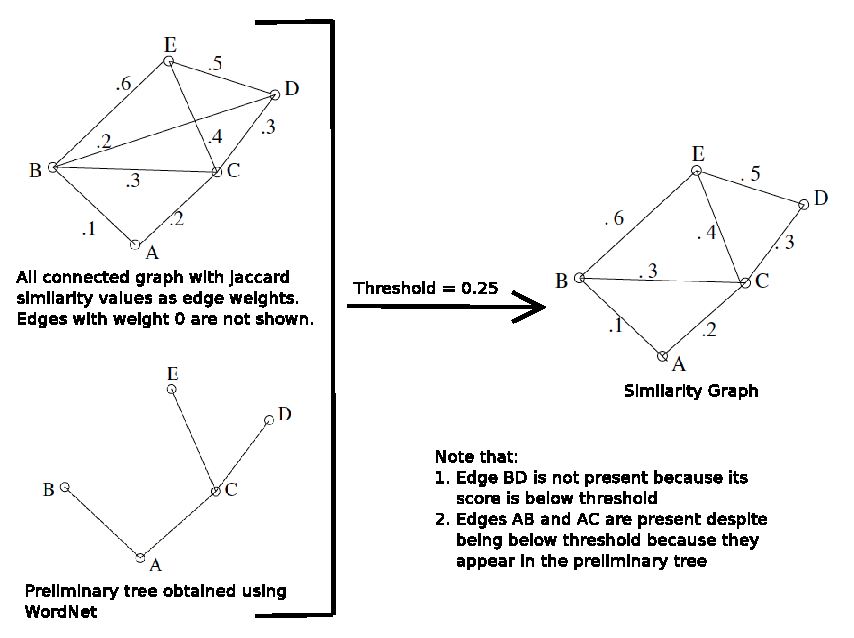
\includegraphics[width=0.8\linewidth]{TagTree/CreatingSimGraph}
\caption{Building the Similarity Graph for threshold $\tau$=0.25} 
\label{fig:sim}
\end{figure}
%\subsection{Objective Function} \label{subsec:objfunction}
Given the similarity graph $\mathcal{G_T}$, the objective of the refinement stage is to find a tree in the space of spanning trees of the similarity graph $\mathcal{G_T}$ which minimizes a defined objective function. Below we define and motivate two different objective functions based on corpus statistics, for tag tree construction. 
\begin{enumerate}
\item \textbf{Weighted Average Hops (WAH)}: 
\begin{equation}
\; \sum_i\sum_{j, j < i}{J_{\mathcal{T}}(i,j)d_{i,j}} , 
\label{eq:ObjFnWeightedHops}
\end{equation}
where $d_{i,j}$ represents the number of hops between tag $t_i$ and tag $t_j$ in the tag tree. The motivation for such a score is that it is lower when tags $i$ and $j$ with high $J_{\mathcal{T}}(i,j)$ are separated by fewer hops as compared to tags with low $J_{\mathcal{T}}(i,j)$. \hl{The above objective function is equal to the sum of the pair-wise hops between all pairs of tags weighted by the corresponding Jaccard similarity {$J_{\mathcal{T}}(i,j)$}. Dividing the sum by 
$\sum_{i,j < i}{J_{\mathcal{T}}(i,j)}$ would be equal to the weighted average number of pair-wise hops where the weights are normalized Jaccard similarities. Since the value $\sum_{i,j <  i} {J_{\mathcal{T}}(i,j)}$ is a constant for a given set of tags {$\mathcal{T}$}, we have removed the scaling factor from the objective function. }
For a general graph $\mathcal{G_T}$, the problem of minimizing the weighted average number of hops has been established to be an NP hard problem \cite{garey1979computers}.  
\item \textbf{Similarity Approximation (SA)}: 
\begin{equation}
\; \sum_i\sum_{j, j < i}{w_{i,j}\mid J_{\mathcal{T}}(i,j) - S_T{(i,j)}} \mid  , \\
\label{eq:ObjFnSimApprox}
\end{equation}
where $S_T{(i,j)}$ represents the similarity between tags $t_i$ and $t_j$ estimated using tag tree $T$. A very close problem is that of approximating a given distance matrix through spanning trees, which has been established to be NP hard~\cite{eckhardt2005combinatorial}. The objective function in~(\ref{eq:ObjFnSimApprox}) is the weighted L1 norm of the difference between the Jaccard Matrix $J_{\mathcal{T}}$ and the \textbf{Estimated Similarity Matrix} $S_T$. \hl{The weights $w_{i,j}$ are taken to be the co-occurrence counts of tags $t_i$ and $t_j$ and are useful to establish relative importances between different pairs of tags in the objective function}. While $S_T{(i,j)}$ can be calculated in several ways for a given tag tree $T$, we define $S_T{(i,j)}$  as 
\begin{equation}
S_T{(i,j)} = \prod_{e \in \mathfrak{P}_{i,j}}{S(e)}  , \\
\label{eq:ProdSimSimilarityCalculate}
\end{equation}
where $\mathfrak{P}_{i,j}$ is the path in tag tree $T$ connecting tags $t_i$ and $t_j$ and $S(e)$ is equal to the Jaccard similarity between the tags that edge $e$ connects. Such a definition for $S_T{(i,j)}$  ensures that it lies between 0 and 1 and no rescaling is required in order to compare $S_T{(i,j)}$  values with $J_{\mathcal{T}}(i,j)$.
\end{enumerate}
\hl{Note that the trees in ({\ref{eq:ObjFnWeightedHops}}) and ({\ref{eq:ObjFnSimApprox}}) are constrained to be spanning trees over the Similarity Graph $\mathcal{G_T}$. }The local search based approach to minimize either of the above objective functions is described next. 
\vspace{-0.12in}
\subsection{Optimization based on Local Search}
\label{subsec:localsearch}
\comment{
\noindent In this section we describe the construction of the tree. We split this process into the following two steps:
\begin{enumerate}
%\item {\bf {\em Constructing a similarity graph}}: We define a similarity metric for each pair of tags and threshold it appropriately to obtain a binary feature. i.e. we will call a tag pair {\bf {\em ``similar''}} iff their similarity score is greater than a threshold $t$. This is then used to build a similarity graph $\mathcal{G_t}$ where the vertices correspond to the tags and the edges correspond to tag pairs that are similar.
\item {\bf {\em Constructing a similarity graph}}: We start with the tree on the set of tags built using the WordNet database. We define a similarity metric for each pair of tags and threshold it appropriately to obtain a binary relation. i.e. we will call a tag pair {\bf {\em ``similar''}} iff their similarity score is greater than a threshold $t$. We then add the edges corresponding to similar tag pairs to the original tree and obtain the similarity graph which we will denote by $\mathcal{G_t}$.
\item {\bf {\em Building an optimized tree}}: On the set $\mathcal{S}$ of spanning trees of $\mathcal{G_t}$, we define a neighbour relation and a potential function and find a minimal tree using the local search paradigm.
\end{enumerate}

\subsection{Similarity Graph}

***** TODO (Chetan) ***** \\
--Fill in details of how initial tree using WordNet is constructed \\
********* \\



*****  TO BE FILLED **************** \\
-- Describe the threshold and the distribution from which it is calculated \\
--  We can't say $t$ is empirically estimated as mean $J(s_1, s_2)$ because that might make spanning trees infeasible \\
******************************************
}
Given the Similarity Graph $\mathcal{G_T}$ for a set of tags $\mathcal{T}$, our objective is to construct a spanning tree on $\mathcal{G_T}$ such that the defined objective function is minimized. Since finding spanning trees of $\mathcal{G_T}$ that optimally minimize either (\ref{eq:ObjFnWeightedHops}) or (\ref{eq:ObjFnSimApprox}) is a hard problem, we propose an approach to obtain local optimum through the local search paradigm. 
\\
\indent \textit{Local Search} -- Local search algorithms provide a local optimum to an optimization problem. This is done by moving from one solution to another, in the search space of candidate solutions. \\
For the problem of constructing a ontological tag tree, we define a simple edge-exchange based  neighborhood on the space of spanning trees of the graph $\mathcal{G_T}$ as follows. Given two spanning trees $T_1$, $T_2$ we say that $T_2$ is a neighbour of $T_1$ iff it can be obtained from $T_1$ by the following process:
\begin{enumerate}
	\item Pick an edge $e_1 \in \mathcal{G_T}\setminus T_1$ and add it to $T_1$. 
	\item In the (unique) cycle thus formed in $T_1$ containing $e_1$ pick the edge, say $e_2$ with minimum weight (i.e., jaccard similarity of the tags $e_2$ connects). Remove $e_2$ from $T_1$. 
\end{enumerate}
Starting from a spanning tree $T_0$ of $\mathcal{G_T}$ as an initial solution, we explore all neighbors of $T_0$ to determine which neighbor minimizes the defined objective function. The winning neighbor is then considered as the next solution and its neighbors are explored until no further benefit is seen in the objective function. The steps of the local search based ontological tree construction are listed in Algorithm~\ref{algo:STCAlgorithm}. The output is the locally optimal tag tree $T_{opt}$. Note that $T_0$ is taken as $T_W$ as obtained from Algorithm~\ref{alg:WordNetSTAlgo}. Fig.~\ref{fig:neighborhood} show one iteration of the proposed local search based approach for the objective function in (\ref{eq:ObjFnWeightedHops}). 
\begin{algorithm}
\fontsize{8pt}{1em}\selectfont
\caption{Ontological Tree Construction Algorithm}
\label{algo:STCAlgorithm} 
\textbf{Input:} \\
$\cdot$ Similarity graph $\mathcal{G_T}$ for a given set of tags $\mathcal{T}$ \\ 
$\cdot$ Initial Solution: $T_0$. \\
$\cdot$ \hl{Pair-wise Jaccard similarities between tags, i.e., $J_{\mathcal{T}}(i,j)$}
\textbf{Initialization:} 
$S$=$T_0$ \\
%$T_0$ can be randomly selected as any spanning tree over $\mathcal{G_T}$, or be picked in a heuristical manner \\
\textbf{Loop: } \\
\hspace*{5mm} $\cdot$ $E_{Candidates}$ := set of edges present in $\mathcal{G_T}$ and not in $S$ 
\hspace*{5mm} \textbf{For each edge $e$ in $E_{Candidates}$} \\
%\hspace*{10mm} (Exploring neighbors of current solution)  \\
\hspace*{10mm} $\cdot$ Add edge $e$ in $S$ to get graph $G$. \\
\hspace*{10mm} $\cdot$ $E_{Cycles}$ :=set of edges in the cycle formed in $G$. \\
\hspace*{10mm} $\cdot$ Remove edge $e'$ with lowest weight (i.e., jaccard \\
\hspace*{10mm} \; similarity of connecting tags) from $E_{Cycles}$: $e' \neq e$ \\
\hspace*{10mm} $\cdot$ $S_{Neighbor}$ = spanning tree thus formed  \\
\hspace*{10mm} $\cdot$ Calculate objective function at $S_{Neighbor}$ \\
\hspace*{5mm} \textbf{EndFor} \\
\hspace*{5mm} $\cdot$ Select neighbor giving best objective function as $S_{Next}$ \\
\hspace*{5mm} $\cdot$ If $S_{Next}$ improves objective function over $S$ \\
\hspace*{10mm} $S=S_{Next}$ \\
\hspace*{5mm} $\cdot$ Else Stop iterating \\ 
\textbf{End Loop}. \textbf{Output:} locally optimal spanning tree $T_{opt}=S$
\end{algorithm}

\begin{figure}[htbp]
\begin{center}
\centering
%\includegraphics[width=0.8\linewidth]{Neighbourhood-2}
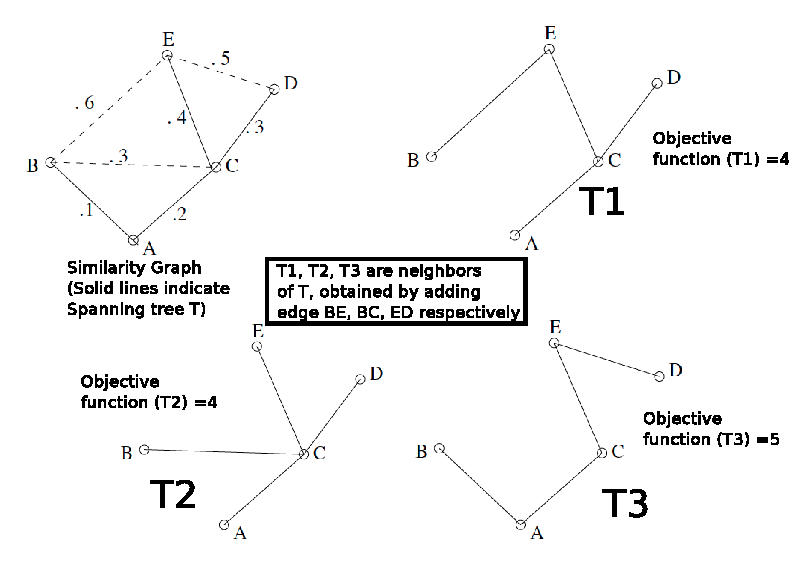
\includegraphics[width=0.8\linewidth]{TagTree/LSOneiteration}
\caption{One iteration of the proposed approach. Eq. (\ref{eq:ObjFnWeightedHops}) is utilized to calculate the objective function for neighbors of a tree T. Ties are broken arbitrarily. Since both T1 and T2 have an objective function~(\ref{eq:ObjFnWeightedHops}) value of 4, we choose T1 and proceed to next iteration. } 
\label{fig:neighborhood}
\end{center}
\end{figure}
% \subsubsection{Optimization Function} 
% \subsubsection{Local Search}
\subsection{Effect of initializing using WordNet}
\comment{
\hl{Utilizing a preliminary tag tree that is constructed using the semantics obtained WordNet has two benefits. Firstly, this biases the constructed structure to have connections dictated by semantic similarity when the data driven relations between certain tags are not strong enough to uniquely determine the structure of the tag tree. The constructed tag tree would thus have edges that are explicable based on the semantic similarity of the tags, as compared to randomness induced as an artefact of the construction procedure. As compared to other tag trees with possibly similar value of the objective function, the resulting tag trees offer a clean interpretation of the relationship between the tags. For example, consider four tags A, B, C, D with pair-wise jaccard similarities as given in Fig. {\ref{fig:ExampleWhyWordnet}}. 
}
\comment{
\begin{table}[htbp]
\scriptsize
\begin{center}
\caption{\hl{Example pair-wise jaccard similarities}}
\label{tab:ExampleWhyWordnet}
%\begin{tabular}{|p{4cm}|p{3.0cm}|}
\begin{tabular}{|c|c|c|c|c|}
		\hline
		 & A & B & C & D \\ 
		\hline 
		A & 1 & 0.9 & 0.1 & 0.3 \\ 
		\hline 
		 B & 0.9 & 1 & 0.2 & 0.2 \\ 
		\hline
		 C & 0.1 & 0.2 & 1 & 0.2 \\
		\hline
		D & 0.3 & 0.2 & 0.2 & 1 \\
		\hline 
\end{tabular}
\end{center}
\end{table}
}
\hl{Based on the first (LS-WAH) objective function ({\ref{eq:ObjFnWeightedHops}}), the two tag trees that would have the same value of the objective function (equal to 2.5) are shown in Fig.~{\ref{fig:whywordnet}} as X and Y. The tag tree as per WordNet is denoted by W. Random initializations of the local search based optimization as detailed in Section {\ref{sec:ConstructionTree}} can lead to either of X or Y as the solution. However initializing using W leads to a unique solution Y where tag B is connected to tags C and D, as in W, thus preferring connections that conform to their semantic relationship. \\
\textbf{Question: Should we even have the first para and its figs?\\ }
} }
\hl{The benefit of using WordNet to initialize the proposed local search based approach is that as compared to random initializations, the former helps achieve a preferred value of the objective function faster. The typical way to attain a lower value of the objective function for an optimization problem as defined in Section {\ref{sec:refinement}} would be to run the local search using randomly constructed tree on the set of tags as initialization, and picking the best tree across several such runs based on the tag tree that has lowest objective function. However this requires running the local search several times which can be large considering that the number of spanning trees on a set of $N$ tags varies as $N^{N-2}$~{\cite{cayley1894collected}}. The preliminary tree as constructed using WordNet offers a more meaningful initialization to the local search by capturing certain types of relationships between the tags that are dictated by their semantics. Table {\ref{tab:WordNetRandominitGWS30}} provides the statistics of the objective function of tag trees constructed by running the proposed local search based approach 20 times with random initializations. As can be seen, a single run using WordNet based preliminary tag tree leads to a much better objective function~({\ref{eq:ObjFnSimApprox}}). Also, the resulting tag tree using WordNet leads to a better performance than the best across 20 runs with random initializations. Note that for Table {\ref{tab:WordNetRandominitGWS30}}, the performance of tag trees is measured using Average Tag Prediction Accuracy as discussed in Section {\ref{sec:Expts}}.} 

\comment{
\begin{figure}[h]
\begin{center}
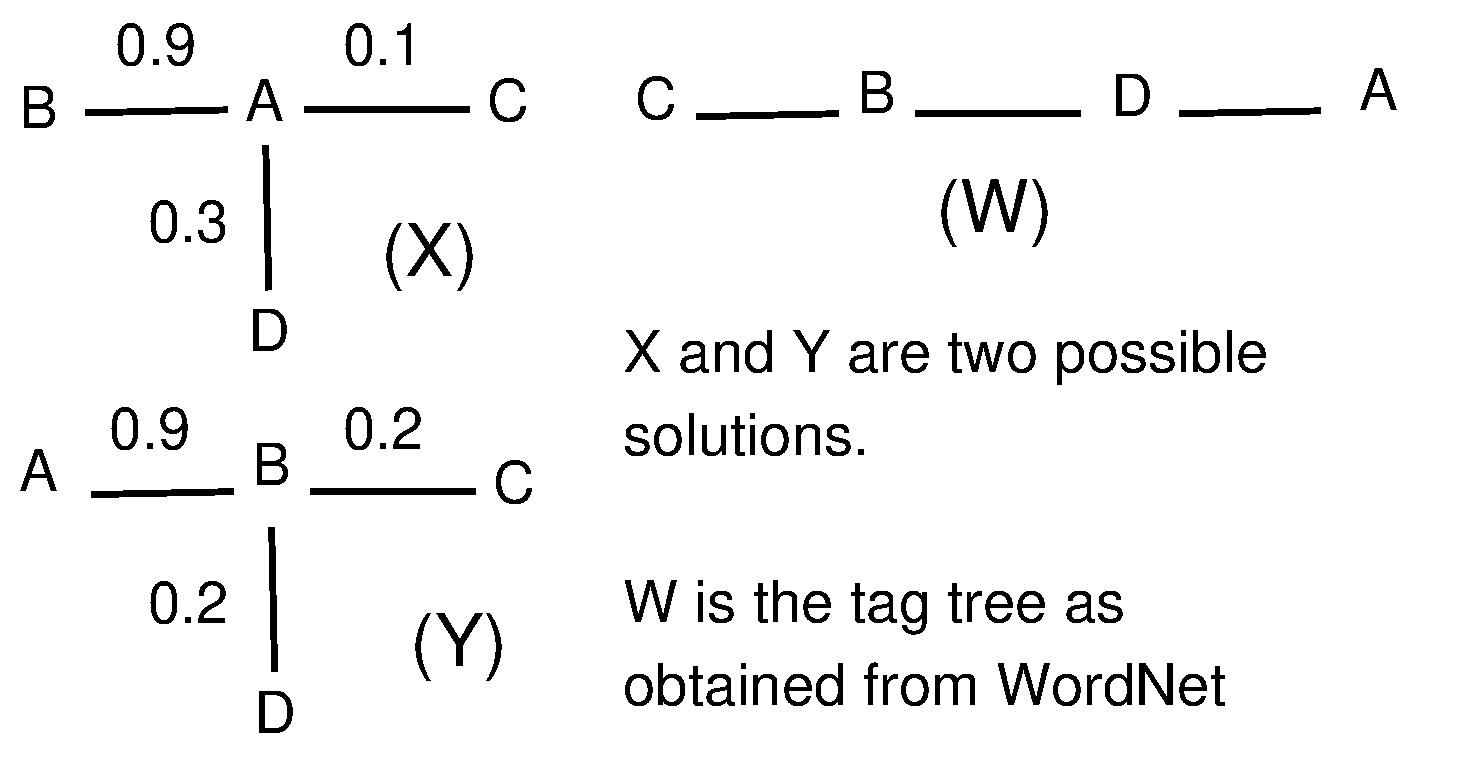
\includegraphics[width=0.65\linewidth]{TagTree/WhyWordNetExample}
\caption{\hl{Example showing multiple solutions using (LS-WAH) objective function ({\ref{eq:ObjFnWeightedHops}}) } }
\label{fig:whywordnet}
\end{center} 
\end{figure}
}
\comment{
\begin{figure}[t!]
\centering
\minipage{0.17\textwidth}
%\centering
  \includegraphics[width=\linewidth]{TagTree/TableWordNetExample.png} 
\caption{\hl{Example pair-wise jaccard similarities}}
\label{fig:ExampleWhyWordnet}
%\end{centering}
\endminipage %\hfill
\hspace{0.1in}
\minipage{0.28\textwidth}
  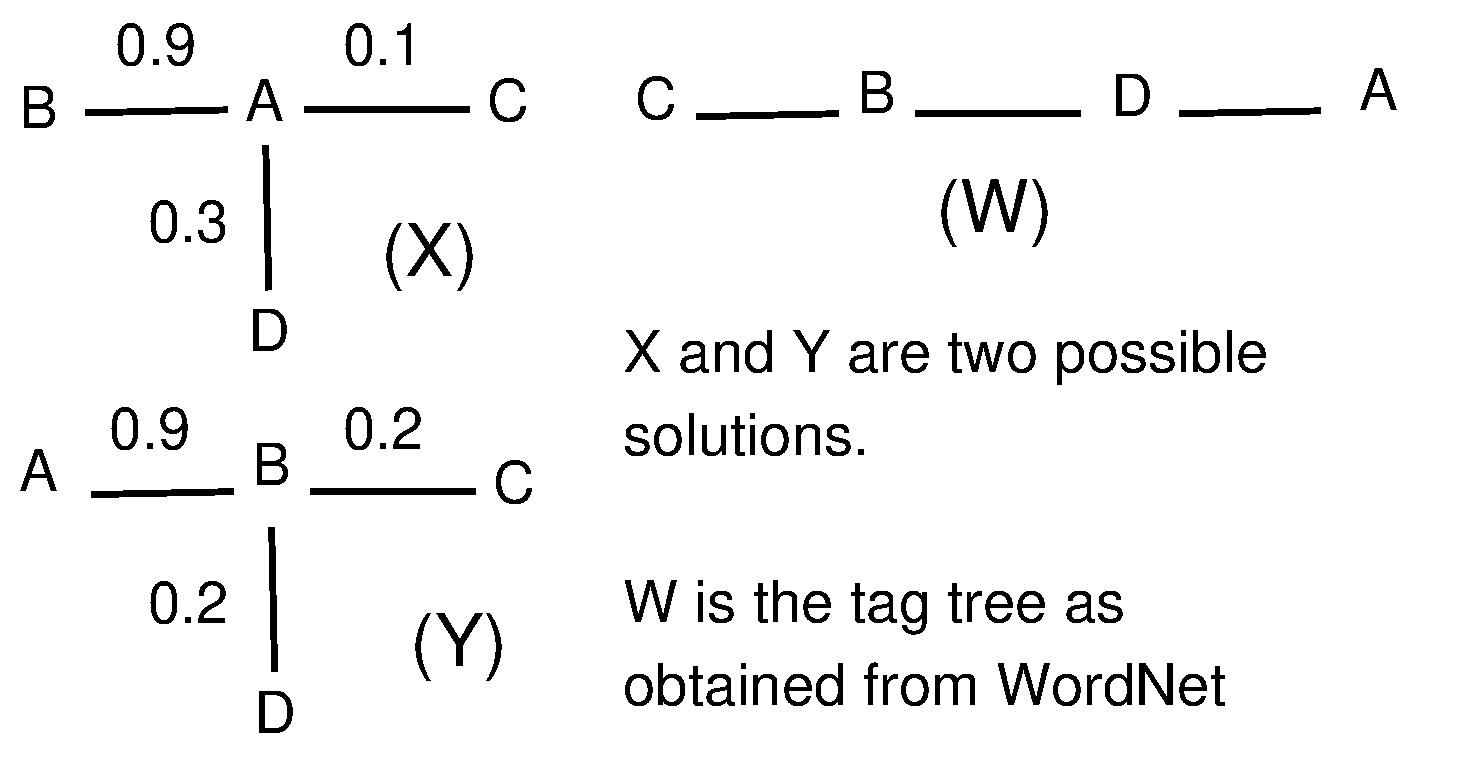
\includegraphics[width=\linewidth]{TagTree/WhyWordNetExample}
\caption{\hl{Example showing multiple solutions using (LS-WAH) objective function ({\ref{eq:ObjFnWeightedHops}}) } }
\label{fig:whywordnet}
\endminipage %\hfill
\end{figure}
}
\begin{table}[htbp]
%\scriptsize
\begin{center}
\caption{Effect of initializing the proposed local search based approach using WordNet. 30 tags from stock image corpus (described in Section IV) are used. }
\label{tab:WordNetRandominitGWS30}
\begin{tabular}{lllll}
\toprule 
     & \multicolumn{3}{c}{Random initialization} & \multicolumn{1}{c}{Using WordNet}\\

    & Min & Mean & Max & \multicolumn{1}{c}{}  \\
    \midrule
    Objective function ((4) x $10^6$) & 6.4    & 13.7  &  47.7  & \multicolumn{1}{c}{0.6} \\
    Performance (in \%) & 24.2    &43.8  & 49.2  & \multicolumn{1}{c}{50.9} \\
    \bottomrule
\end{tabular}
\end{center}
\end{table}
\section{Evaluation} 
\label{sec:Expts}
In this section, we describe the experimental setup for the construction and evaluation of ontological tag trees. For the evaluation, we define tag prediction and efficient classification tasks as discussed later in this section. The experiments are conducted on two large corpora of images, the details of which are given below.  
\vspace{-0.1in}
\subsection{Datasets} 
\label{sec:Datasets}
To test the robustness of our approach to build ontological tag trees for domains with varying degrees of tag noise, we use two different image corpora - one from Flickr, composed primarily of user generated content, and one from a professionally curated stock photo agency.
\begin{itemize} 
\item \textbf{Flickr images}: Flickr~\cite{Flickr} is a popular image and video hosting website where users can upload images and associate them with annotations such as titles, tags and descriptions, among others. As Flickr primarily contains user generated content, tags are often noisy, irrelevant to image content or even completely absent. 
%As can be seen in Fig.~\ref{fig:CDFFlickr}, more than 90\% Flickr images have 13 or less tags associated with them. 
We utilize 500,000 images for training and 100,000 images for testing. All these images are licensed under Creative Commons copyright licenses.
\item \textbf{Stock images corpus}: To evaluate the proposed approach on less noisy data, we take a corpus of stock photos that are professionally annotated, and hence are accompanied with a variety of accurate annotations - such as keywords, captions, etc. For this corpus, we use the set of keywords to build the ontological tag tree, and refer to them as "tags".
%Images are professionally annotated and hence 90\% of Getty images have 38 or less tags (Fig.~\ref{fig:CDFGetty}), which is much more than in the case of Flickr. 
We utilize more than 350,000 images for training and close to 70,000 images for testing. The textual captions are used in the efficient classification task as shown in Section~\ref{sec:effClassification}.
\end{itemize} 

Training images are used for adapting the WordNet based preliminary tag tree obtained using Algorithm~\ref{alg:WordNetSTAlgo} to the given corpus using the local search based approach described in Algorithm~\ref{algo:STCAlgorithm}. Training images are also used for specific required tasks such as training of classifiers. Testing images are used to evaluate the constructed tag trees. There is no overlap between training and test sets.



\subsection{Effect of Local Search based Optimization}
We first demonstrate how the proposed local search based approach helps in improving the objective function as defined in Section~\ref{sec:ConstructionTree}. Fig.~\ref{fig:ObjFun} shows the variation of the objective function in (\ref{eq:ObjFnWeightedHops}) with the number of iterations on Flickr tag corpus. The objective function value of the WordNet based preliminary tag tree for Flickr corpus before the proposed refinement is $357.2$ that becomes $167.1$ using the local search based refinement in $68$ iterations. Median of the Jaccard similarity values is taken as the threshold $\tau$ for candidate selection in the proposed refinement algorithm. Similar improvement is observed for the Stock images corpus, for which the objective function values improves from $224.5$ to $99$ after 23 iterations. For both corpora, the iterations are terminated once no further improvement is observed in the objective function. We describe below the tasks defined to evaluate the constructed tag trees. 
\begin{figure}[h!]
\begin{center}
%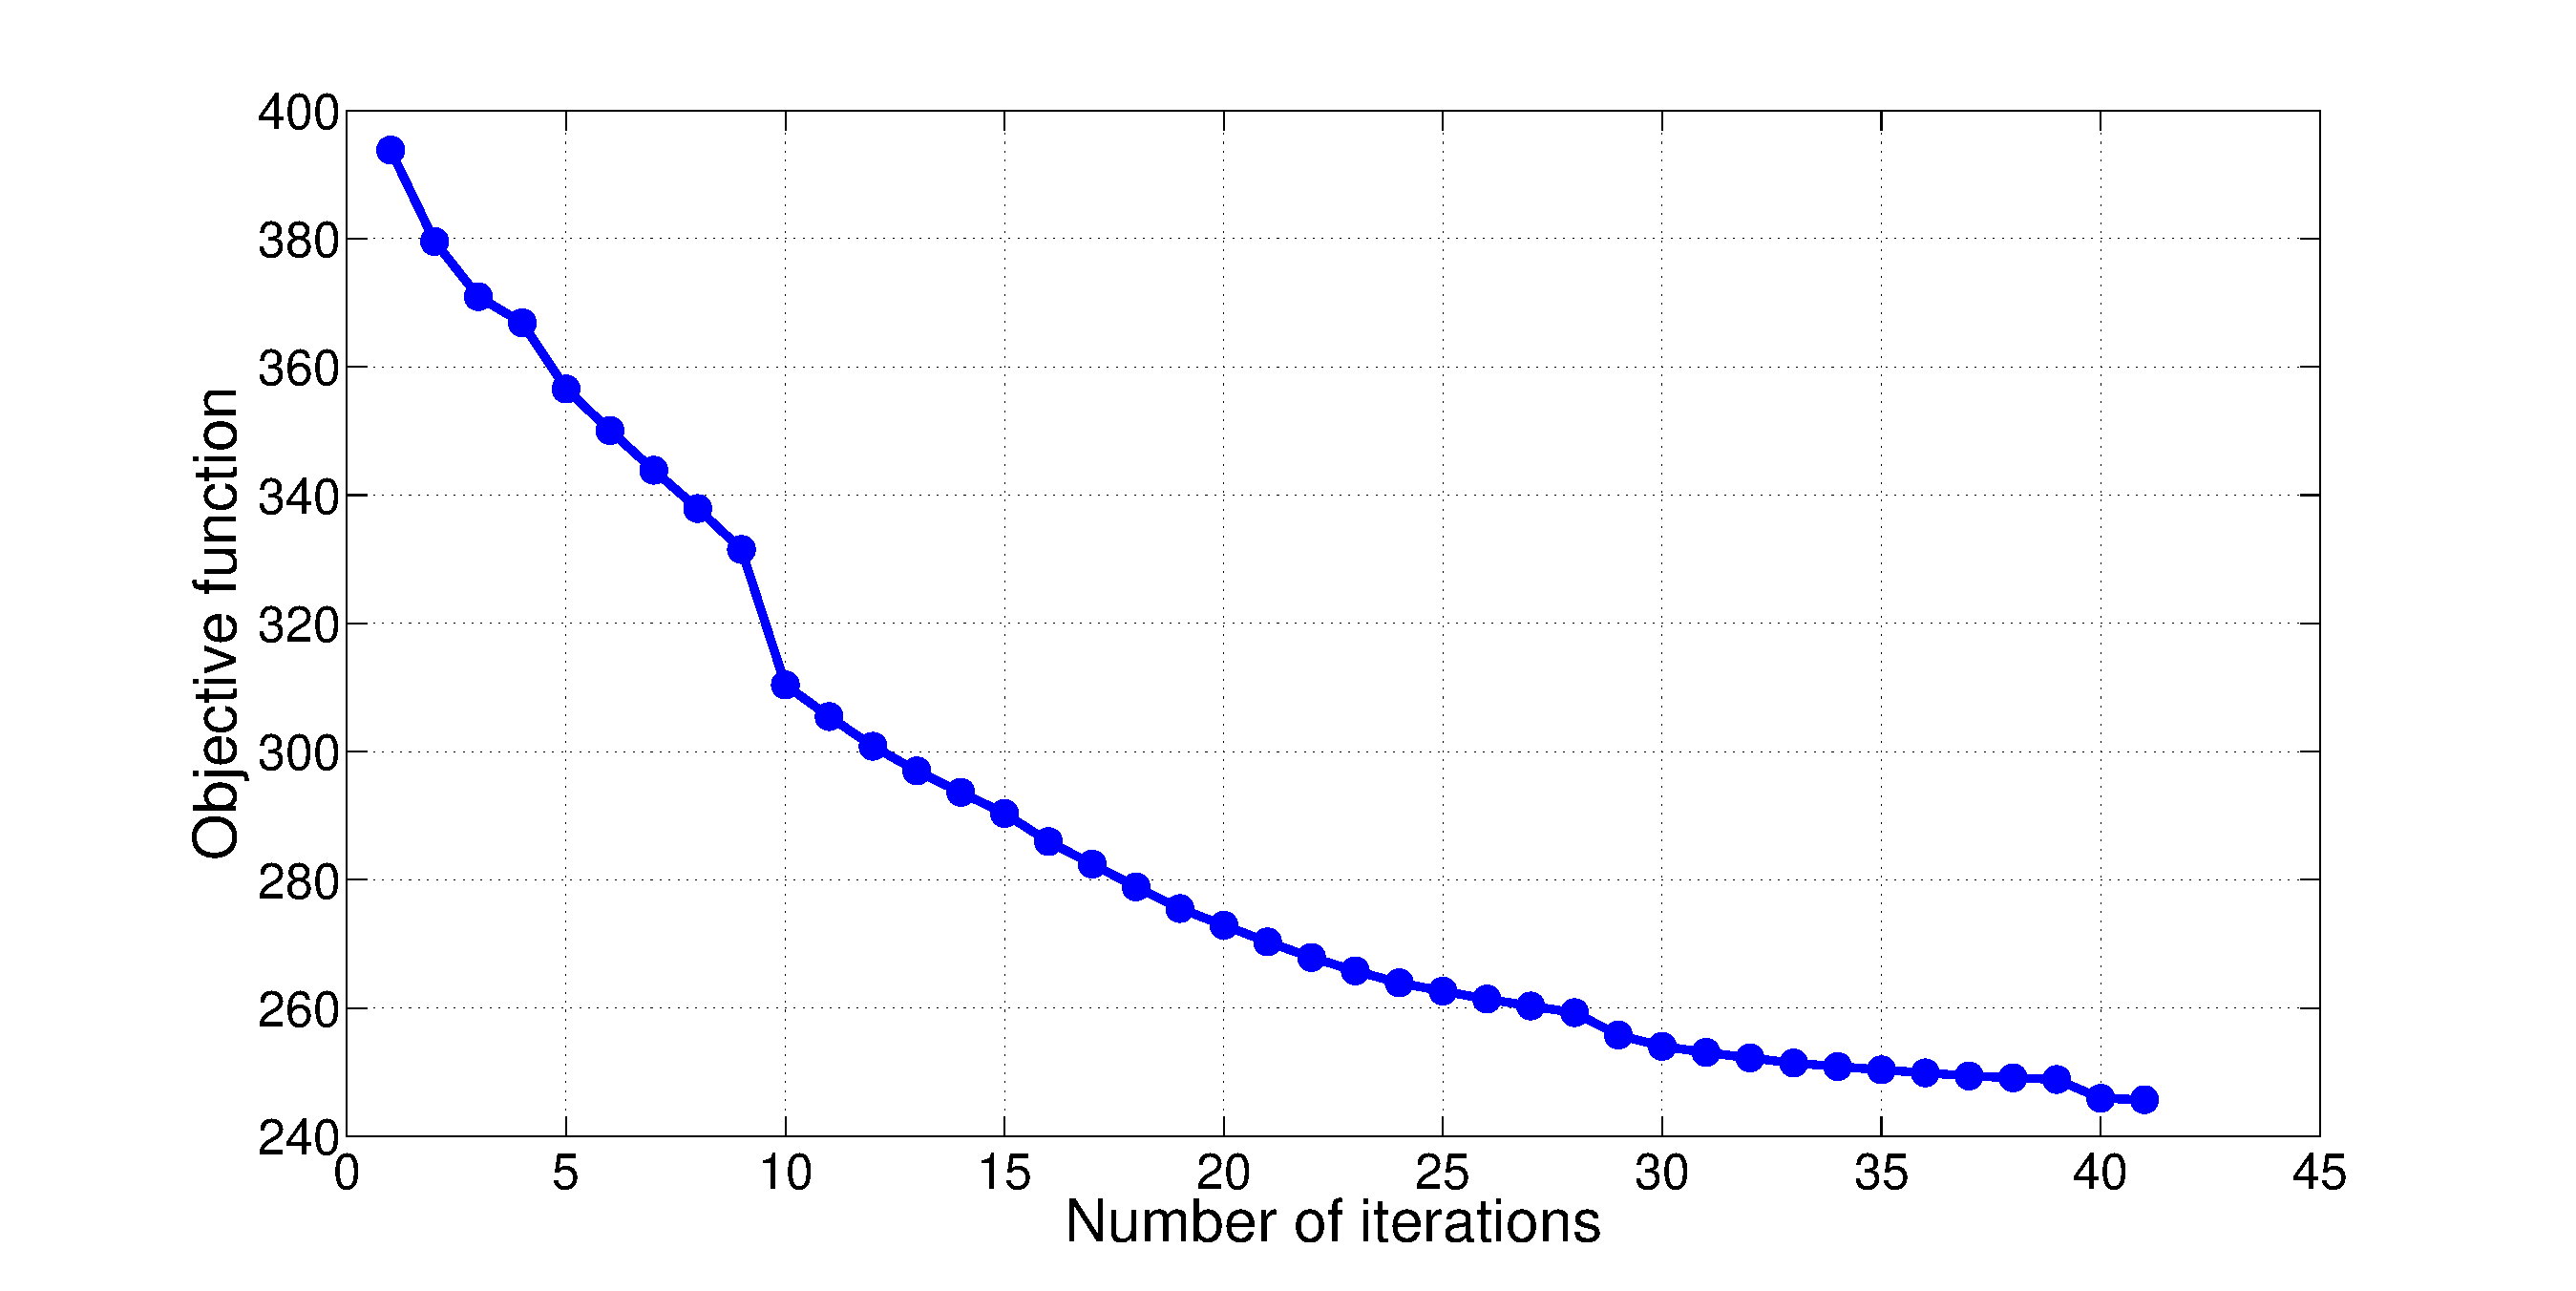
\includegraphics[width=0.8\linewidth]{TagTree/SigmaCijDijVariatPerIter999point05STGD}
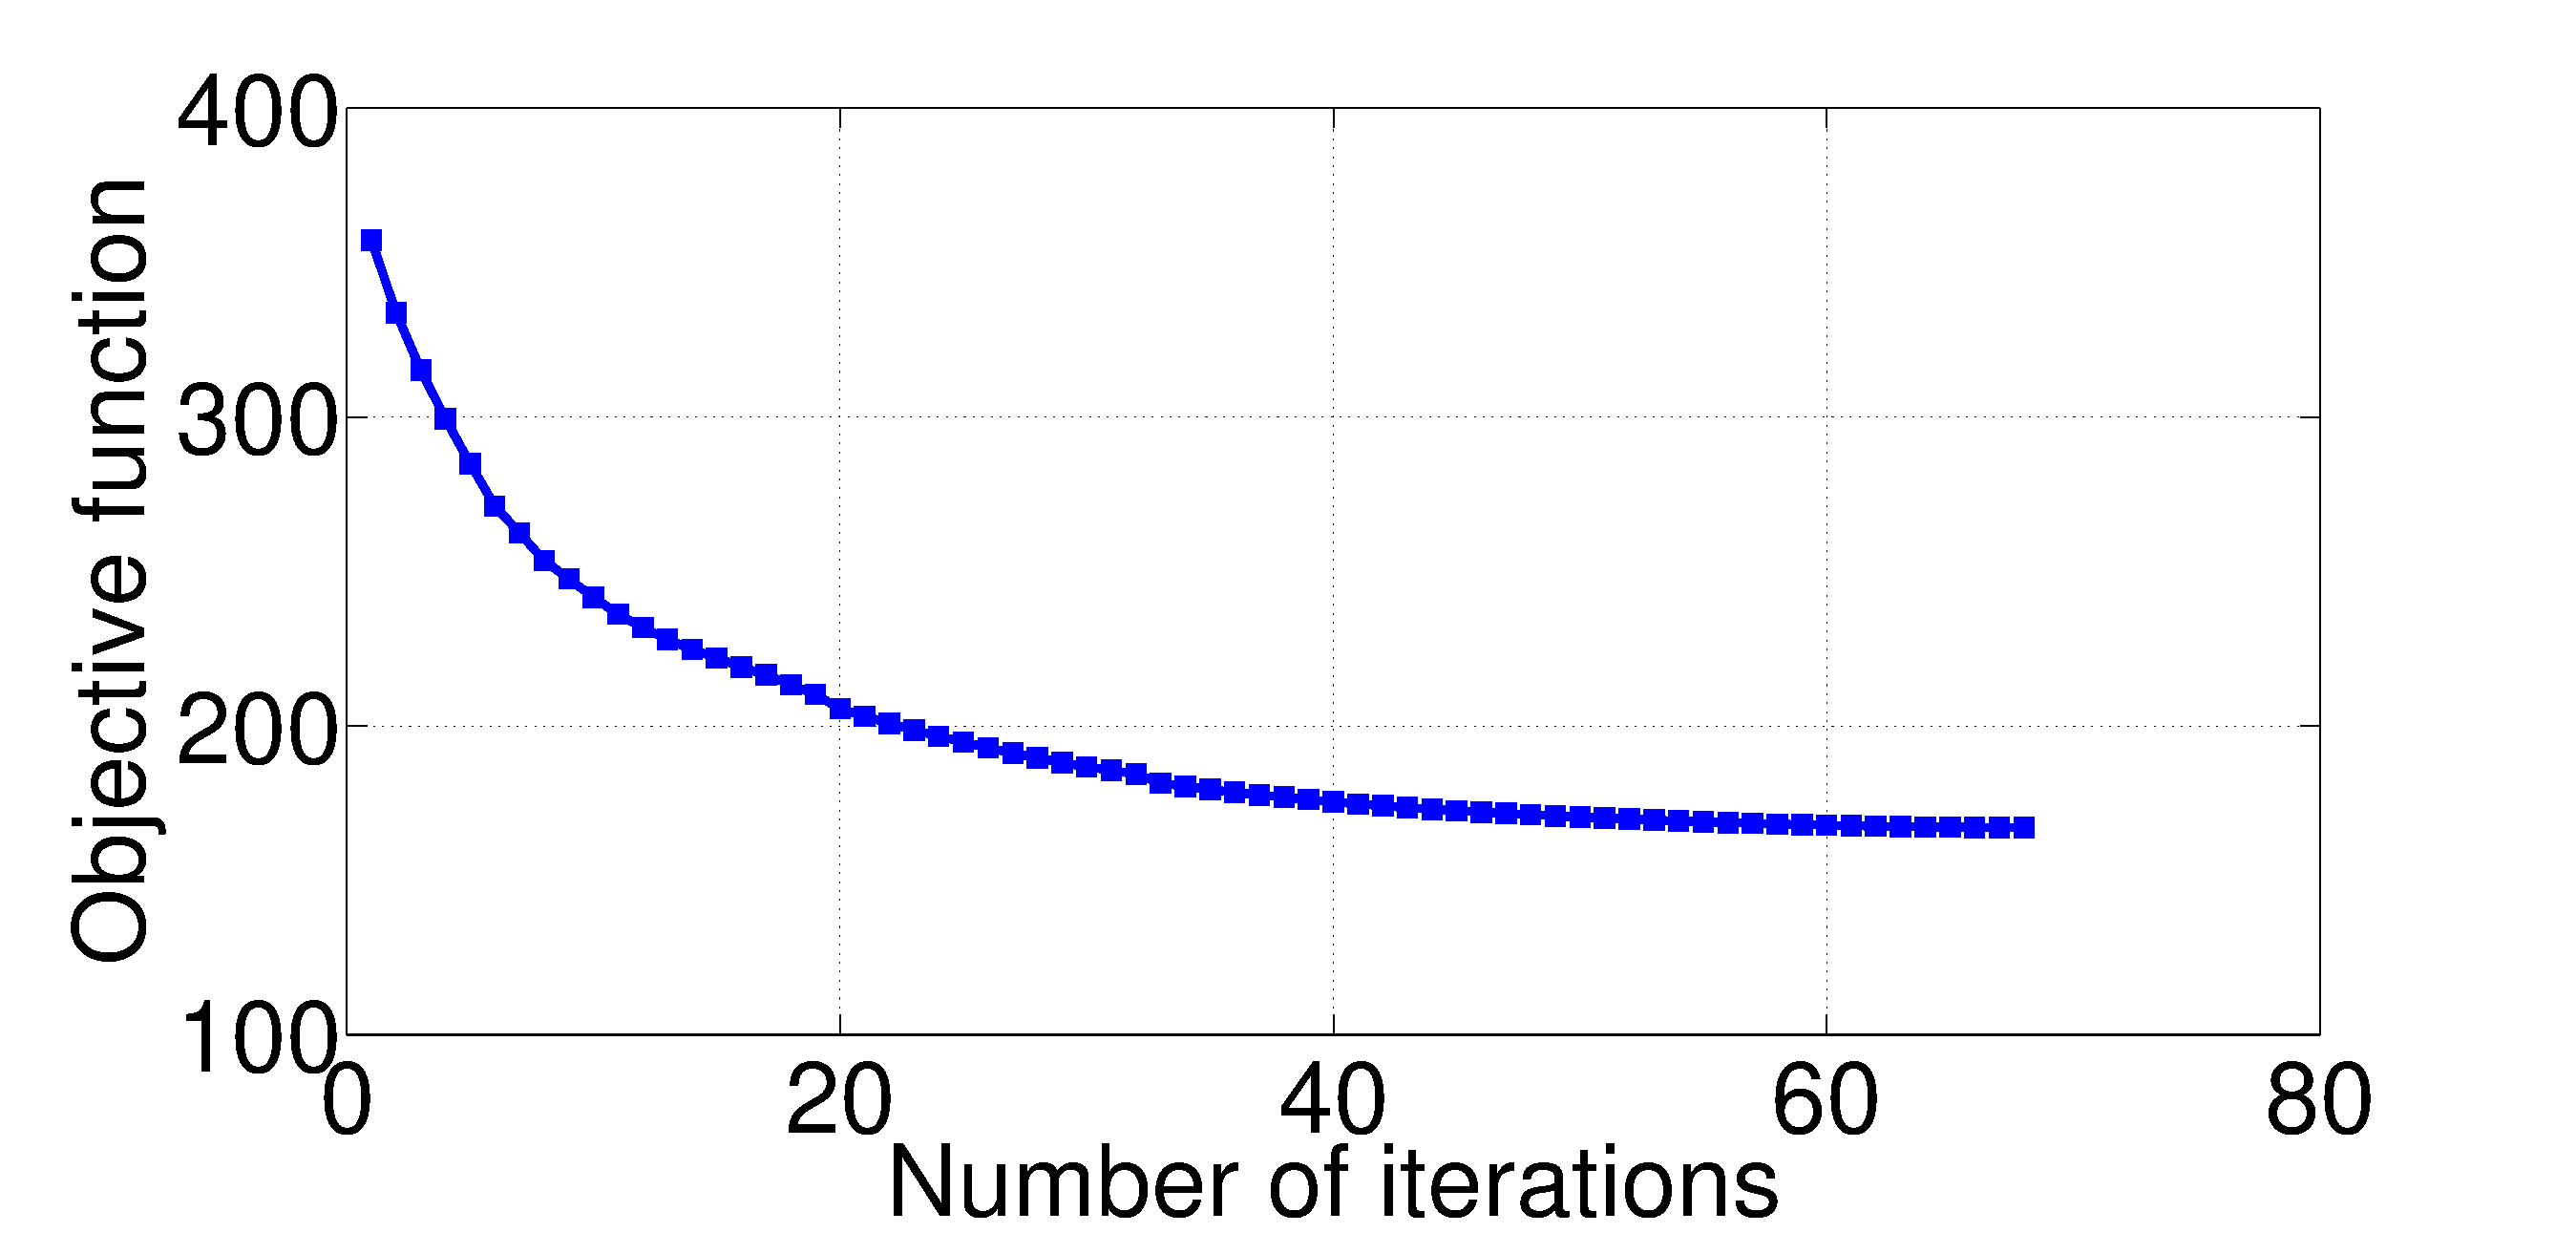
\includegraphics[width=0.65\linewidth]{TagTree/LSWWW_objectivefnValuePerIteration}
\caption{The variation of the objective function~(\ref{eq:ObjFnWeightedHops}) with the number of iterations for a sample run on Flickr tag corpus.} 
\label{fig:ObjFun}
\end{center}
\end{figure}
%We describe below the tasks defined to evaluate the constructed tag trees. 
% \indent \textit{Subsumption-based Semantic Graph} - \cite{SubsumptionText} and \cite{SubsumptionFlickr} utilize a rule-based subsumption model to derive hierarchies from text corpus and Flickr respectively. We utilize the same model to construct hierarchy for keywords of interest, and construct semantic graph by disregarding parent-child relationships and keeping only the edges. \\ 
% \indent We evaluate the performance of a semantic graph by utilizing the graph to assist in classification as detailed below. 
\subsection{Tag Prediction Task} 
\label{subsec:TagPred}
%The intuition behind this task is that a semantic graph that provides better performance in tag prediction is able to capture the information that characterizing the corpus in a much better manner. 
%Tag prediction is performed with the help of a given graph as detailed below. 
 
\hl{The tag prediction task is similar to the tag recommendation task in  {\cite{katsurai2013cross}} and in {\cite{sigurbjornsson2008flickr}}. However as outlined in Section {\ref{sub_sec:relatedWork}}, the proposed task does not require manual labeling for the resources (images) to evaluate the proposed tag tree construction approach. In order to do so, we divide the tags associated with a resource into a seen and an an unseen set of tags and use the latter to evaluate the predicted tags. We demonstrate this approach through experiments conducted on image corpora. 
}
Let an image $i$ in the corpus be tagged with the set of tags $\mathcal{T}_i$, such that $\mid \mathcal{T}_i \mid =N_{Tags}$. Assume that out of these $N_{Tags}$ tags, only a subset $\mathcal{T}_{i,Seen}$ are observed, with $\mid \mathcal{T}_{i,Seen} \mid=N_{Seen}$. The objective of the \emph{tag prediction task} is to predict the remaining ($N_{Tags} - N_{Seen}$) tags, i.e., $\mathcal{T}_i \setminus \mathcal{T}_{i,Seen}$.  Let $\mathbb{P}_i$ be the set of ($N_{Tags} - N_{Seen}$) tags predicted for image $i$ assuming that $\mathcal{T}_{i,Seen}$ is observed. Note that the prediction assumes the total number of tags for the image, $N_{Tags}$, to be known. Performance of tag prediction can be measured by the \emph{Tag Prediction Accuracy}, defined as follows: 
\begin{equation} \label{eq:TagPredAccuracy}
%\text{Tag Prediction Score} = \frac{\mid  \{\mathcal{T}_i \setminus  \mathcal{T}_{i,Seen}\} \cap \mathbb{P}_i \mid}{ \mid \{  \mathcal{T}_i \setminus  \mathcal{T}_{i,Seen} \}  \cup \mathbb{P}_i \mid} .
\text{Tag Prediction Accuracy} = \frac{\mid  \{\mathcal{T}_i \setminus  \mathcal{T}_{i,Seen}\} \cap \mathbb{P}_i \mid}{ \mid \{  \mathcal{T}_i \setminus  \mathcal{T}_{i,Seen} \} \mid} .
\end{equation} 

We now discuss the approach we follow to obtain the set of predicted tags $\mathbb{P}_i$ when the set of tags $\mathcal{T}_{i,Seen}$ is seen, by utilizing a given ontological tag tree. 
\subsubsection{Utilizing Ontological Tag Tree for Tag Prediction} 
\label{sec:TagPredUsingGraph}
Consider the tag tree $T$, built over the set of $\mathcal{T}$ tags in a corpus. For image $i$ with $N_{Seen}$ number of seen tags, each tag $t \in \{ \mathcal{T} \setminus \mathcal{T}_{i,Seen} \}$ is given a proximity score $s_t$ based on its proximity from the seen tags, as per $T$. Specifically, 
\begin{equation} 
s_t = \Sigma_{t' \in \mathcal{T}_{i,Seen} }{dist(t,t')}, 
\label{eq:TPEquation}
\end{equation}
where $dist(t,t')$ is the distance between tags $t$ and $t'$ in $T$ calculated as shown in Section~\ref{sec:comparison}. A lower proximity score for a tag $t$ indicates that it is closer in a cumulative sense to the set of observed tags $\mathcal{T}_{i,Seen}$. The tags are ordered in the increasing order of $s_t$, and the first ($N_{Tags} - N_{Seen}$) tags, i.e. those corresponding to the least values of $s_t$, are chosen as the set of predicted tags $\mathbb{P}_i$. \\

\subsubsection{Methods Compared} 
\label{sec:comparison}
We compare the following methods in the tag prediction task:
\begin{enumerate}
\item \underline{Random}: As the name suggests, this baseline method randomly picks  ($N_{Tags} - N_{Seen}$)  tags from the set $\mathcal{T} \setminus \mathcal{T}_{i,Seen}$. 

\item \underline{WordNet}: This baseline approach uses the semantics based ontological tag tree constructed from WordNet hierarchy using the procedure described in Algorithm 1. The edge weights are assigned to be semantic distances as obtained from \cite{RitaLibraryWordNet}. 
%\item \underline{(Weighted) WordNet hierarchy}: Same as the previous approach with the only difference being that semantic WordNet distances are used as edge weights instead of assigning them to $1$.
\item \underline{Google Similarity Distance}:  Google Similarity Distance \cite{cilibrasi2007google} has been used to construct tag graphs in applications such as tag ranking \cite{liu2009tag}. As mentioned in Section~\ref{sub_sec:relatedWork}, a threshold is used to discard certain edges in tag graphs. We choose a threshold such that for a tag graph with $N$ nodes (or tags), there are exactly $(N-1)$ edges remaining, so that the tag graph thus formed has same number of edges and space requirement as the tag tree learnt from proposed approach. Edge weights for the tag graph are taken to be the Google Similarity Distance as defined in \cite{cilibrasi2007google}. 

%In the approach, we obtain the tag graph based on the Google Distance model~\cite{SubsumptionFlickr}. In order to compare against the proposed approach, this is converted to an ontological graph by ignoring the directions and connecting the node with highest degree in each disconnected components, to a ``Root" node. The resulting subsumption graph is a spanning tree over the set of tags and an additional ``Root" node. 

\item \underline{LS Weighted Average Hops (LS-WAH)}:  Here we construct a tag tree using the proposed local search based approach, to minimize Weighted Average Hops (\ref{eq:ObjFnWeightedHops}) in Section~\ref{sec:refinement}. If an edge exists between tags $t_i$ and $t_j$ then the weight of the edge connecting them is given to be $(1-J_{\mathcal{T}}(i,j))$. 

\item \underline{LS Similarity Approximation (LS-SA)}:  This tag tree is constructed using the proposed approach with objective corresponding to Similarity Approximation as outlined in (\ref{eq:ObjFnSimApprox}) in Section~\ref{sec:refinement}. The edge weights are assigned as in Method 4 above. 

\item \underline{Symmetric sum based}: \hl{In order to compare the performance of the proposed tag tree construction approaches with that of other tag recommendation approaches that do not use tag trees or tag graphs or any visual features, we also provide the performance of the symmetric sum based approach as proposed in {\cite{sigurbjornsson2008flickr}}. Note that the space required to store the pair-wise similarities in {\cite{sigurbjornsson2008flickr}} is $O(N^2)$ while the proposed tag tree construction requires $O(N)$ space to store the tag tree. 
}


%For all present edges in the constructed tree, the weight of the edge is taken to be the jaccard similarity of the connecting tags. 

%\item \underline{LS on WordNet hierarchy}: This approach uses the refined ontological graph obtained using the proposed local search based algorithm (Algorithm 2). The edge weights are assigned to $1$ in this variant of the approach. 

%\item \underline{(Weighted) LS on WordNet hierarchy}: Same as the previous approach with the only difference being that inverse of Jaccard similarities are used as edge weights instead of assigning them to $1$.

\end{enumerate}
The prediction task is performed using the approach described in section~\ref{sec:TagPredUsingGraph}. For methods numbered 2, 3, and 4 above, $dist(t_i, t_j)$ as required in $(\ref{eq:TPEquation})$ is calculated by adding distances of edges in path connecting tags $t_i$ and $t_j$. For LS-SA method, $dist(t_i, t_j)$ is defined as $\{1- S_T{(i,j)}    \}$ where $S_T{(i,j)}$ is calculated for an ontological tag tree $T$ as per $(\ref{eq:ProdSimSimilarityCalculate})$. This is because the tag tree construction approach for LS-SA method utilizes product based similarity approximation $(\ref{eq:ProdSimSimilarityCalculate})$ and so it is appropriate to use same approach to estimate similarities based on a tree, and hence to calculate $dist(t_i, t_j)$. \hl{Similarly, for Symmetric sum based method {\cite{sigurbjornsson2008flickr}}, $dist(t_i, t_j)$ is defined as $\{1- J_{\mathcal{T}}(i,j)    \}$ where $J_{\mathcal{T}}(i,j)$ is the jaccard similarity between tag $t_i$ and $t_j$ as defined in Section~{\ref{sec:refinement}}. Note that this makes ({\ref{eq:TPEquation}}) similar to the sum based scoring approach in {\cite{sigurbjornsson2008flickr}}. 
}

%\indent The tag prediction task is conducted on two corpora, Flickr and the stock images corpus. We present the results in detail below. \\
\comment{
\begin{figure*}[!ht]
\minipage{0.32\textwidth}
  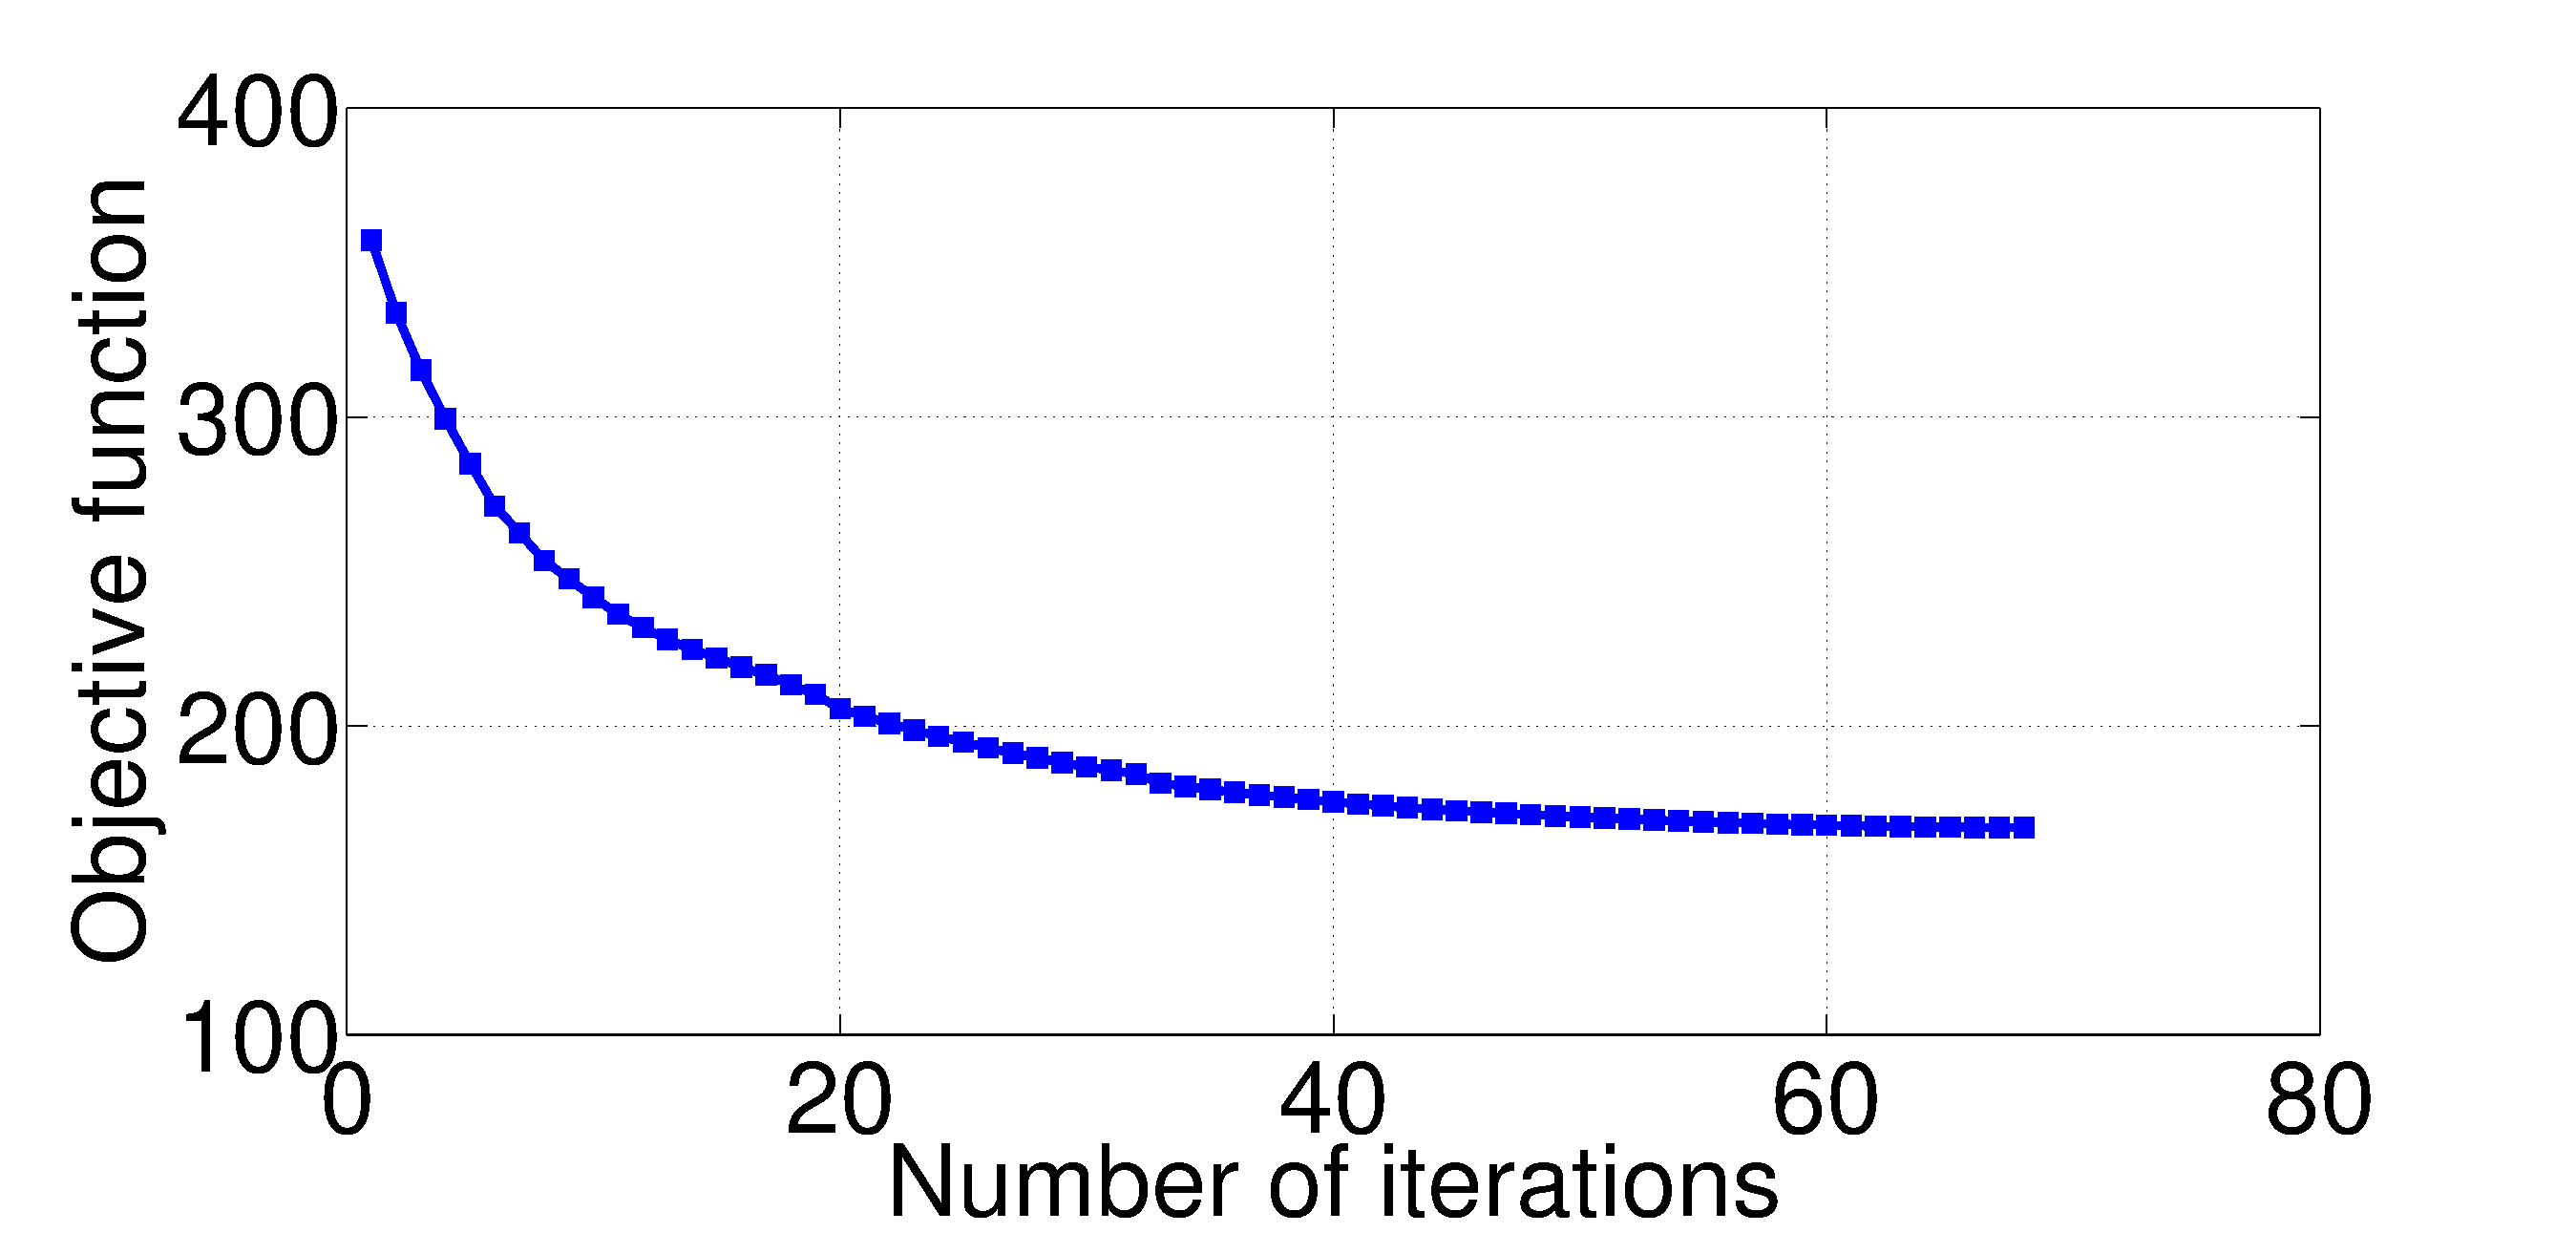
\includegraphics[width=\linewidth]{TagTree/LSWWW_objectivefnValuePerIteration}
\caption{The variation of the objective function~(\ref{eq:ObjFnWeightedHops}) with the number of iterations for a sample run on Flickr tag corpus.} 
\label{fig:ObjFun}
\endminipage\hfill
\minipage{0.32\textwidth}
  \includegraphics[width=\linewidth]{TPFlickr_rebuttal}
\caption{\hl{Average Tag Prediction Accuracies marginalized over $N_{Tags}$ for various methods for the tag prediction task on Flickr corpus. }} 
\label{fig:FWS117TagPredGraph}
\endminipage\hfill
\minipage{0.32\textwidth}%
  \includegraphics[width=\linewidth]{RebuttalGWS_TP}
\caption{\hl{Average Tag Prediction Accuracies marginalized over $N_{Tags}$ for various methods for the tag prediction task on Stock images corpus.}}
\label{fig:GWS30TagPredGraph}
\endminipage
\end{figure*}
}
\textbf{Flickr corpus:} We begin by choosing  the top $150$ most popular tags in a sample of Flickr images. After selecting only those tags that also occur in the WordNet database, we are left with 117 tags. These comprise the set $\mathcal{T}$. The total number of tags in an image, varies from 0 to 6 for most Flickr images. Since we need at least one tag to be seen and at least one to be predicted, we vary $N_{Tags}$  from 2 to 6. For each value of $N_{Tags}$, test images are selected which contain exactly $N_{Tags}$ tags. For each such image $i$, all combinations of $N_{Seen}$ tags are selected to comprise the observed tag set $\mathcal{T}_{i,Seen}$. Predictions are made as discussed in Section ~\ref{sec:TagPredUsingGraph} and performance of tag prediction task is measured using~(\ref{eq:TagPredAccuracy}). $N_{Seen}$ is varied from 1 through $(N_{Tags} - 1)$. Given values for $N_{Tags}$ and $N_{Seen}$, the Average Tag Prediction Accuracy is the Tag Prediction Accuracy using (\ref{eq:TagPredAccuracy}) averaged across test images. We define Overall Tag Prediction Accuracy as the mean of Average Tag Prediction Accuracy across all combinations of $N_{Tags}$ and $N_{Seen}$. 

The Overall Tag Prediction Accuracies for the various methods compared are shown in Table ~\ref{tab:TPFlickr117Summary}. Tables \ref{tab:TPFlickr117Random} through \ref{tab:TPFlickr117Jij} show the Average Tag Prediction Accuracies for various combinations of $N_{Tags}$ and $N_{Seen}$ for the individual methods discussed in Section \ref{sec:comparison} for Flickr corpus. For comparison, the Average Tag Prediction Accuracies marginalized over $N_{Tags}$ are shown in Fig.~\ref{fig:FWS117TagPredGraph}. Note that Google Distance refers to the method corresponding to Google Similarity Distance as outlined above. \hl{It can be seen that the LS-SA method outperforms all others and has its performance very close to that of the Symmetric sum based approach {\cite{sigurbjornsson2008flickr}}. It should be noted that the latter utilizes pair-wise similarities between tags as derived from the corpus and thus has space requirement of $O(N^2)$ which as discussed in Section {\ref{sub_sec:relatedWork}} is very high for large number of tags, i.e., for large $N$. Compared to this, the proposed approach has only $O(N)$ space requirement. } We will discuss in Section \ref{sec:Discussion} the reason why LS-SA leads to construction of a tree that outperforms the LS-WAH method. Google distance based method has performance close to that of LS-WAH while the tag tree based on WordNet hierarchy does not work very well for tag prediction task. As expected, random tag prediction performs the worst.
%One interesting observation from Table ~\ref{tab:TPFlickr117Summary} and Fig.~\ref{fig:FWS117TagPredGraph} is that even the unweighted version of ontological tag tree obtained using proposed data-driven approach performs far better than both random prediction and WordNet based graph (both weighted and unweighted). 
%Stating differently, the gain in performance is not merely a manifestation of having corpus-centric edge weights though they do improved the performance obtained for this task.

\comment{
\begin{table}[htbp]
\begin{center}
\caption{Overall Tag Prediction Scores for various methods for the tag prediction task on Flickr corpus. }
\label{tab:TPFlickr117Summary}
%\begin{tabular}{|p{4cm}|p{3.0cm}|}
\begin{tabular}{|c|c|}
		\hline
%		\textbf{Tag Prediction Algorithm} & \textbf{Avg Tag Prediction Score (in \%)}   \\ 
		\textbf{Tag Prediction} & \textbf{Prediction}\\ 
		\textbf{Algorithm} & \textbf{Score (\%)}\\ 
		\hline 
		 Random tag prediction   & 1.63  \\
		\hline
		 WordNet hierarchy & 4.92  \\
		\hline
%		3 & Minimum spanning tree formed using WordNet distances  & 4.7740  \\
%		\hline
%		3 & 2 + Local search using WordNet distances (Needed?) & 7.44  \\
%		\hline
%		5 & 3 + Local Search using WordNet distances (Needed?) & 4.2622  \\
%		\hline
		 (Weighted) WordNet hierarchy  & 5.41  \\
		\hline
%		7 & 3 + Edge Weights (WordNet Distances)  & 5.1941  \\
%		\hline
%		8 & 4 + Edge Weights (WordNet Distances) (Needed?) & Pending  \\
%		\hline
%		9 & 5 + Edge Weights (WordNet Distances)  (Needed?) & Pending  \\
%		\hline
%		5 & 2 + Edge weights (Inverse of Jaccard Similarity) & 6.9   \\  
%		\hline
%		10 & 3 + Edge weights (Inverse of Jaccard Similarity) & ---  \\
%		\hline
		 LS on WordNet hierarchy & 28.61  \\
		\hline
%		11 & 3 + Local Search using Jaccard Similarity & 18.1985  \\
%		\hline
		 (Weighted) LS on WordNet hierarchy   &  35.75  \\
		\hline
%		13 & 11 + Edge Weights (Inverse Jaccard Similarity)   & 32.9313  \\
%		\hline
%		11 & 8 + Edge Weights (WordNet Distances)   & ---  \\
%		\hline
%		12 & 9 + Edge Weights (WordNet Distances)   & ---  \\ 
%		\hline
\end{tabular}
\end{center}
\end{table}
}

\begin{table}[htbp]
\fontsize{8pt}{1em}\selectfont
%\scriptsize
\begin{center}
\caption{Overall Tag Prediction Accuracy (\%) for various methods for tag prediction task on Flickr and Stock images corpora. }
\label{tab:TPFlickr117Summary}
%\begin{tabular}{|p{4cm}|p{3.0cm}|}
\begin{tabular}{|c|c|c|}
		\hline
		\textbf{Tag Prediction} & \textbf{Flickr} & \textbf{Stock images} \\ 
		\textbf{Method} & \textbf{corpus} & \textbf{corpus}\\ 
		\hline 
		 Random tag prediction   & 2.29  & 13.21 \\
		\hline
		 WordNet  & 7.95  & 22.67 \\
		\hline
		Google Similarity Distance & 34.02 & 40.05\\
		\hline 
		 LS - WAH &  31.53  & 48.06\\
		\hline
		LS - SA &  44.52 & 50.86 \\
		\hline
		\hl{Symmetric sum based} &  \hl{47.13} & \hl{54.71} \\
		\hline
\end{tabular}
\end{center}
\end{table}
%\vspace{-5mm}
\begin{figure}[htbp]
%\epsfig{width=9cm,figure=FWS117TagPredResultsusingSTForCol.eps}
%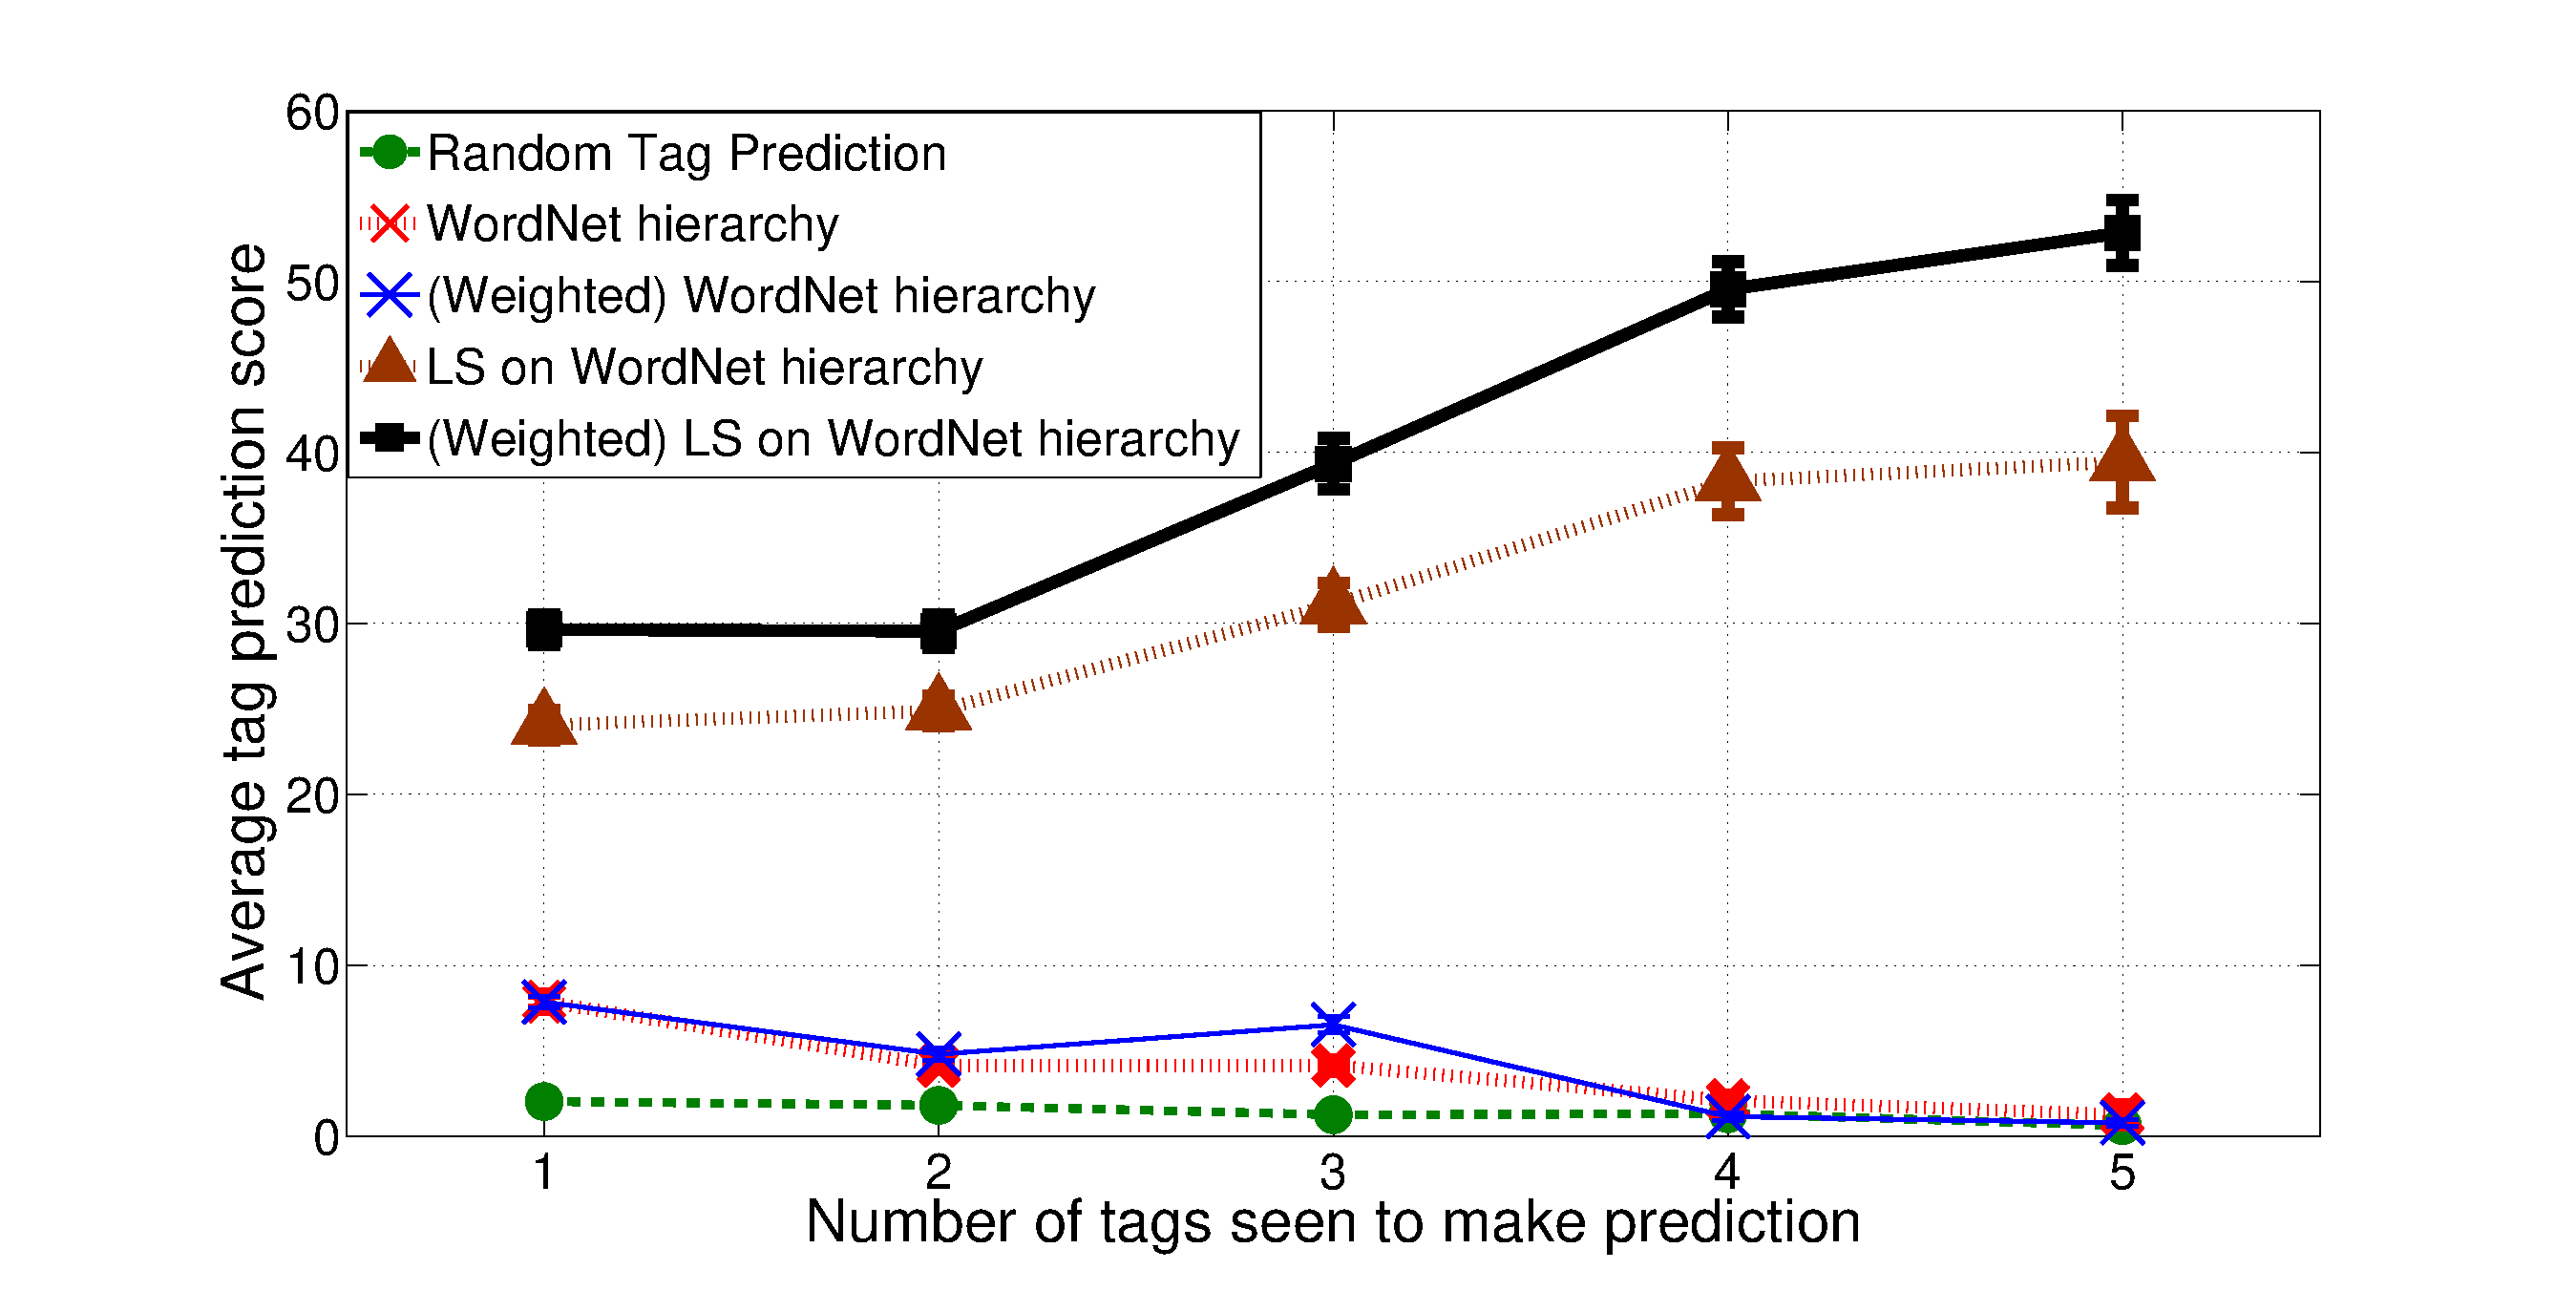
\includegraphics[width=\linewidth]{FWS117TagPredResultsusingSTForCol}
%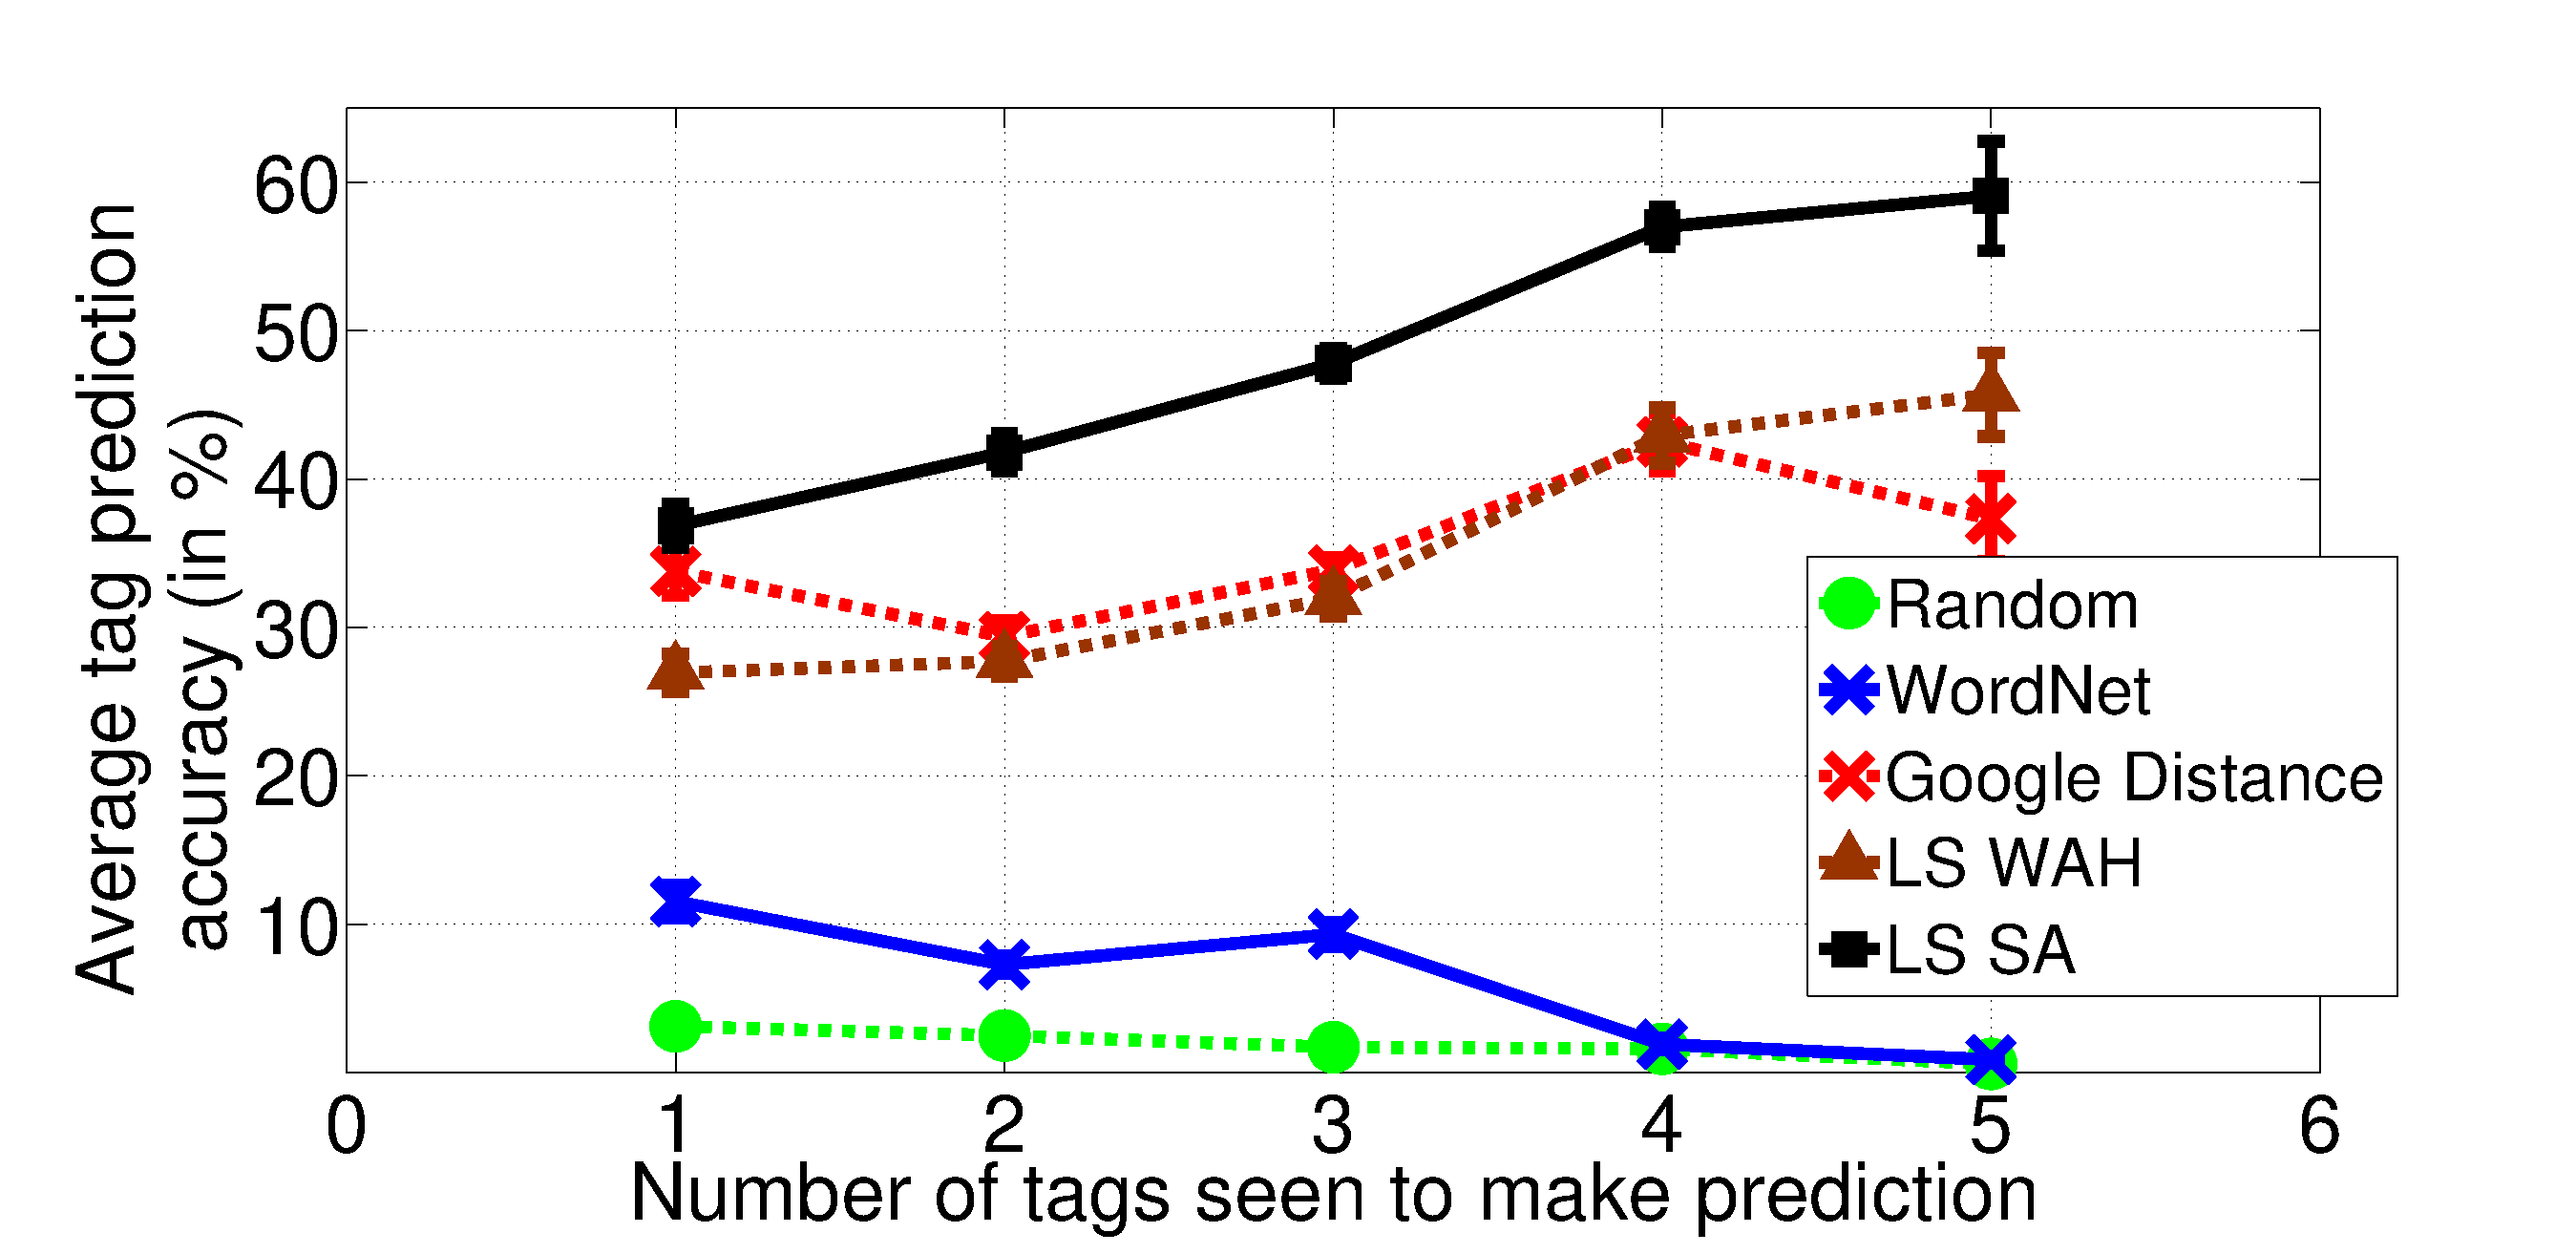
\includegraphics[width=\linewidth]{FlickrTPFig_journal}
\centering
\includegraphics[width=0.65\linewidth]{TagTree/TPFlickr_rebuttal}
\caption[Average Tag Prediction Accuracies marginalized over $N_{Tags}$ for various methods for the tag prediction task on Flickr corpus. ]{Average Tag Prediction Accuracies marginalized over $N_{Tags}$ for various methods for the tag prediction task on Flickr corpus. Note that Google Distance refers to the method corresponding to Google Similarity Distance as outlined in Section \ref{sec:comparison}.} 
\label{fig:FWS117TagPredGraph}
\end{figure}
\begin{table}
\fontsize{8pt}{1em}\selectfont
\begin{center}
\caption{Average Tag Prediction Accuracies (in \%) obtained using  Random method on Flickr corpus.}
%\vspace{-0.2in}
\label{tab:TPFlickr117Random}
\begin{tabular}{|p{2cm}|c|c|c|c|c|}
		\hline
		{$\boldsymbol{N_{Seen} \rightarrow}$} & &  &  &  &\\ 
		{$\boldsymbol{N_{Tags}} \downarrow $} & \textbf{1} & \textbf{2} & \textbf{3} & \textbf{4} & \textbf{5}   \\ 
		\hline 		
		\textbf{2} & 1.57 & - & - & - & -\\ 
		\hline
		\textbf{3} & 2.34 & 1.30 & - & - & -\\ 
		\hline
		\textbf{4} & 2.67 & 1.55 & 0.73 & - & -\\ 
		\hline
		\textbf{5} & 2.19 & 1.68 & 1.01 & 0.78 & -\\ 
		\hline
		\textbf{6} & 6.80 & 5.39 & 3.36 & 2.41 & 0.58 \\ 
		\hline
\end{tabular}
\vspace{-2mm}
\end{center}
\end{table}
\begin{table}
\fontsize{8pt}{1em}\selectfont
\begin{center}
\caption{Average Tag Prediction Accuracies (in \%) obtained using WordNet method on Flickr corpus.} 
\label{tab:TPFlickr117Wordnet}
\begin{tabular}{|p{2cm}|c|c|c|c|c|}
		\hline
		{$\boldsymbol{N_{Seen} \rightarrow}$} & &  &  &  &\\ 
		{$\boldsymbol{ N_{Tags}} \downarrow$} & \textbf{1} & \textbf{2} & \textbf{3} & \textbf{4} & \textbf{5}   \\ 	
		\hline
		\textbf{2} & 7.05 & - & - & - & -\\ 
		\hline
		\textbf{3} & 8.17 & 2.88 & - & - & -\\ 
		\hline
		\textbf{4} & 11.16 & 5.27 & 5.39 & - & -\\ 
		\hline
		\textbf{5} & 16.50 & 10.05 & 13.10 & 0.84 & -\\ 
		\hline
		\textbf{6} & 14.72 & 10.85 & 9.46 & 2.97 & 0.87 \\ 
		\hline
\end{tabular}
\vspace{-2mm}
\end{center}
\end{table}
\begin{table}
\fontsize{8pt}{1em}\selectfont
\begin{center}
\caption{Average Tag Prediction Accuracies (in \%) obtained using Google Similarity Distance method on Flickr corpus.} 
\label{tab:TPFlickr117Google}
\begin{tabular}{|p{2cm}|c|c|c|c|c|}
		\hline
		{$\boldsymbol{N_{Seen} \rightarrow}$} & &  &  &  &\\ 
		{$\boldsymbol{ N_{Tags}} \downarrow$} & \textbf{1} & \textbf{2} & \textbf{3} & \textbf{4} & \textbf{5}   \\ 	
		\hline
		\textbf{2} & 22.07 & - & - & - & -\\ 
		\hline
		\textbf{3} & 17.01 & 5.50 & - & - & -\\ 
		\hline
		\textbf{4} & 23.70 & 16.67 & 11.66 & - & -\\ 
		\hline
		\textbf{5} & 51.51 & 47.09 & 45.28 & 43.15 & -\\ 
		\hline
		\textbf{6} & 54.55 & 48.28 & 44.68 & 41.85 & 37.30 \\ 
		\hline
\end{tabular}
\vspace{-2mm}
\end{center}
\end{table}
\begin{table}[!htb]
\fontsize{8pt}{1em}\selectfont
\begin{center}
\caption{Average Tag Prediction Accuracies (in \%) obtained using LS-WAH method on Flickr corpus.} 
\label{tab:TPFlickr117LSWAH}
\begin{tabular}{|p{2cm}|c|c|c|c|c|}
		\hline
		{$\boldsymbol{N_{Seen} \rightarrow}$} & &  &  &  &\\ 
		{$\boldsymbol{ N_{Tags}} \downarrow$} & \textbf{1} & \textbf{2} & \textbf{3} & \textbf{4} & \textbf{5}   \\ 	
		\hline
		\textbf{2} & 16.13 & - & - & - & -\\ 
		\hline
		\textbf{3} & 11.53 & 5.51 & - & - & -\\ 
		\hline
		\textbf{4} & 14.91 & 10.96 & 7.17 & - & -\\ 
		\hline
		\textbf{5} & 42.76 & 42.94 & 39.69 & 36.95 & -\\ 
		\hline
		\textbf{6} & 49.37 & 51.48 & 49.00 & 48.89 & 45.69 \\ 
		\hline
\end{tabular}
\vspace{-2mm}
\end{center}
\end{table}
\begin{table}[!htb]
\fontsize{8pt}{1em}\selectfont
\begin{center}
\caption{Average Tag Prediction Accuracies (in \%) obtained using LS-SA method on Flickr corpus.}
\label{tab:TPFlickr117LSSA}
\begin{tabular}{|p{2cm}|c|c|c|c|c|}
		\hline
		%\textbf{$N_{Tags}$, $N_{Seen}$} & \textbf{1} & \textbf{2} & \textbf{3} & \textbf{4} & \textbf{5} \\ 
		{$\boldsymbol{N_{Seen} \rightarrow}$} & &  &  &  &\\ 
		{$\boldsymbol{N_{Tags}}\downarrow $} & \textbf{1} & \textbf{2} & \textbf{3} & \textbf{4} & \textbf{5}   \\ 
		\hline 		
		\textbf{2} & 25.87 & - & - & - & -\\ 
		\hline
		\textbf{3} & 20.34 & 21.65 & - & - & -\\ 
		\hline
		\textbf{4} & 26.09 & 28.96 & 26.43 & - & -\\ 
		\hline
		\textbf{5} & 52.33 & 54.79 & 54.82 & 53.16 & -\\ 
		\hline
		\textbf{6} & 59.57 & 61.78 & 62.10 & 60.81 & 59.07 \\ 
		\hline
\end{tabular}
\vspace{-2mm}
\end{center}
\end{table}
\begin{table}[!htb]
\fontsize{8pt}{1em}\selectfont
\begin{center}
\caption{\hl{Average Tag Prediction Accuracies (in \%) obtained using Symmetric sum method on Flickr corpus.}}
\label{tab:TPFlickr117Jij}
\begin{tabular}{|p{2cm}|c|c|c|c|c|}
		\hline
		%\textbf{$N_{Tags}$, $N_{Seen}$} & \textbf{1} & \textbf{2} & \textbf{3} & \textbf{4} & \textbf{5} \\ 
		{$\boldsymbol{N_{Seen} \rightarrow}$} & &  &  &  &\\ 
		{$\boldsymbol{N_{Tags}}\downarrow $} & \textbf{1} & \textbf{2} & \textbf{3} & \textbf{4} & \textbf{5}   \\ 
		\hline 		
		\textbf{2} &\hl{ 25.62} & - & - & - & -\\
		\hline
		\textbf{3} & \hl{21.19} & \hl{22.17} & - & - & - \\
		\hline
		\textbf{4} & \hl{28.69} & \hl{30.88} & \hl{28.12} & - & - \\
		\hline
		\textbf{5} & \hl{55.6} & \hl{57.88} & \hl{57.12} & \hl{54.27} & - \\
		\hline
		\textbf{6} & \hl{62.77} & \hl{65.48} & \hl{67.05} & \hl{66.35} & \hl{63.75} \\
		\hline
\end{tabular}
\vspace{-2mm}
\end{center}
\end{table}


%For completeness, we also provide the Average Tag Prediction Scores for various combinations of $N_{Tags}$ and $N_{Seen}$ in Tables~\ref{tab:TPFlickr117Random} - Table~\ref{tab:TPFlickr117GDWordNetSTJaccardWeight}. It is clear that the proposed approach greatly improves the performance compared to the WordNet based methods for all combinations of $N_{Tags}$ and $N_{Seen}$.
We provide examples of some test images from the Flickr corpus that had $N_{Tags}$=5 and $N_{Seen}$=2. Fig.~\ref{fig:positiveExs} shows a few test images for which LS-SA method made 100\% correct predictions. Fig. \ref{fig:negativeExs} shows test images that gave 0\% tag prediction accuracies. The corresponding sets of seen ($\mathcal{T}_{i,Seen}$), unseen ($\mathcal{T}_i \setminus  \mathcal{T}_{i,Seen}$), and the predicted tags ($\mathbb{P}_i$) are also provided. 


%Table~\ref{tab:TPFlickr117WordNetST}, the Average Tag Prediction Score for  $N_{Tags}=5$ and $N_{Seen}=3$ is only about 4.1\%. Compare this to the score obtained by proposed approach, as shown in Table~\ref{tab:TPFlickr117GDWordNetST}: 40.3\%! 





\textbf{Stock images corpus:} As in the Flickr corpus, we first select the set of most popular tags from the corpus of stock images that are also in WordNet. This produces a set $\mathcal{T}$, of 30 tags. Tables \ref{tab:TPGWS30Random} through \ref{tab:TPGWS30Jij} show the Average Tag Prediction Accuracies for various combinations of $N_{Tags}$ and $N_{Seen}$ for the tag prediction methods discussed in Section \ref{sec:comparison}. 
The Average Tag Prediction Accuracies marginalized over $N_{Tags}$ are shown in  Fig.~\ref{fig:GWS30TagPredGraph}, plotted as a function of $N_{Seen}$.  
%The total number of tags in an image, $N_{Tags}$ is varied from 2 to 10 such that $N_{Seen}$ varies from 1 to ($N_{Tags}-1$).  
Note that if $N_{Tags}$ is kept constant, increasing $N_{Seen}$ reduces the number of unseen tags (i.e., $\mathcal{T}_i \setminus  \mathcal{T}_{i,Seen}$), thus reducing the random chance of predicting a correct unseen tag from $\mathcal{T} \setminus \mathcal{T}_{i,Seen}$.  As a result of this phenomenon, a drop in performance for random prediction and other methods can be seen with increasing $N_{Seen}$. \\
\begin{figure}[!ht]
%\epsfig{width=10cm,figure=GWS20TagPredColumnMeanResultsForST.eps}
%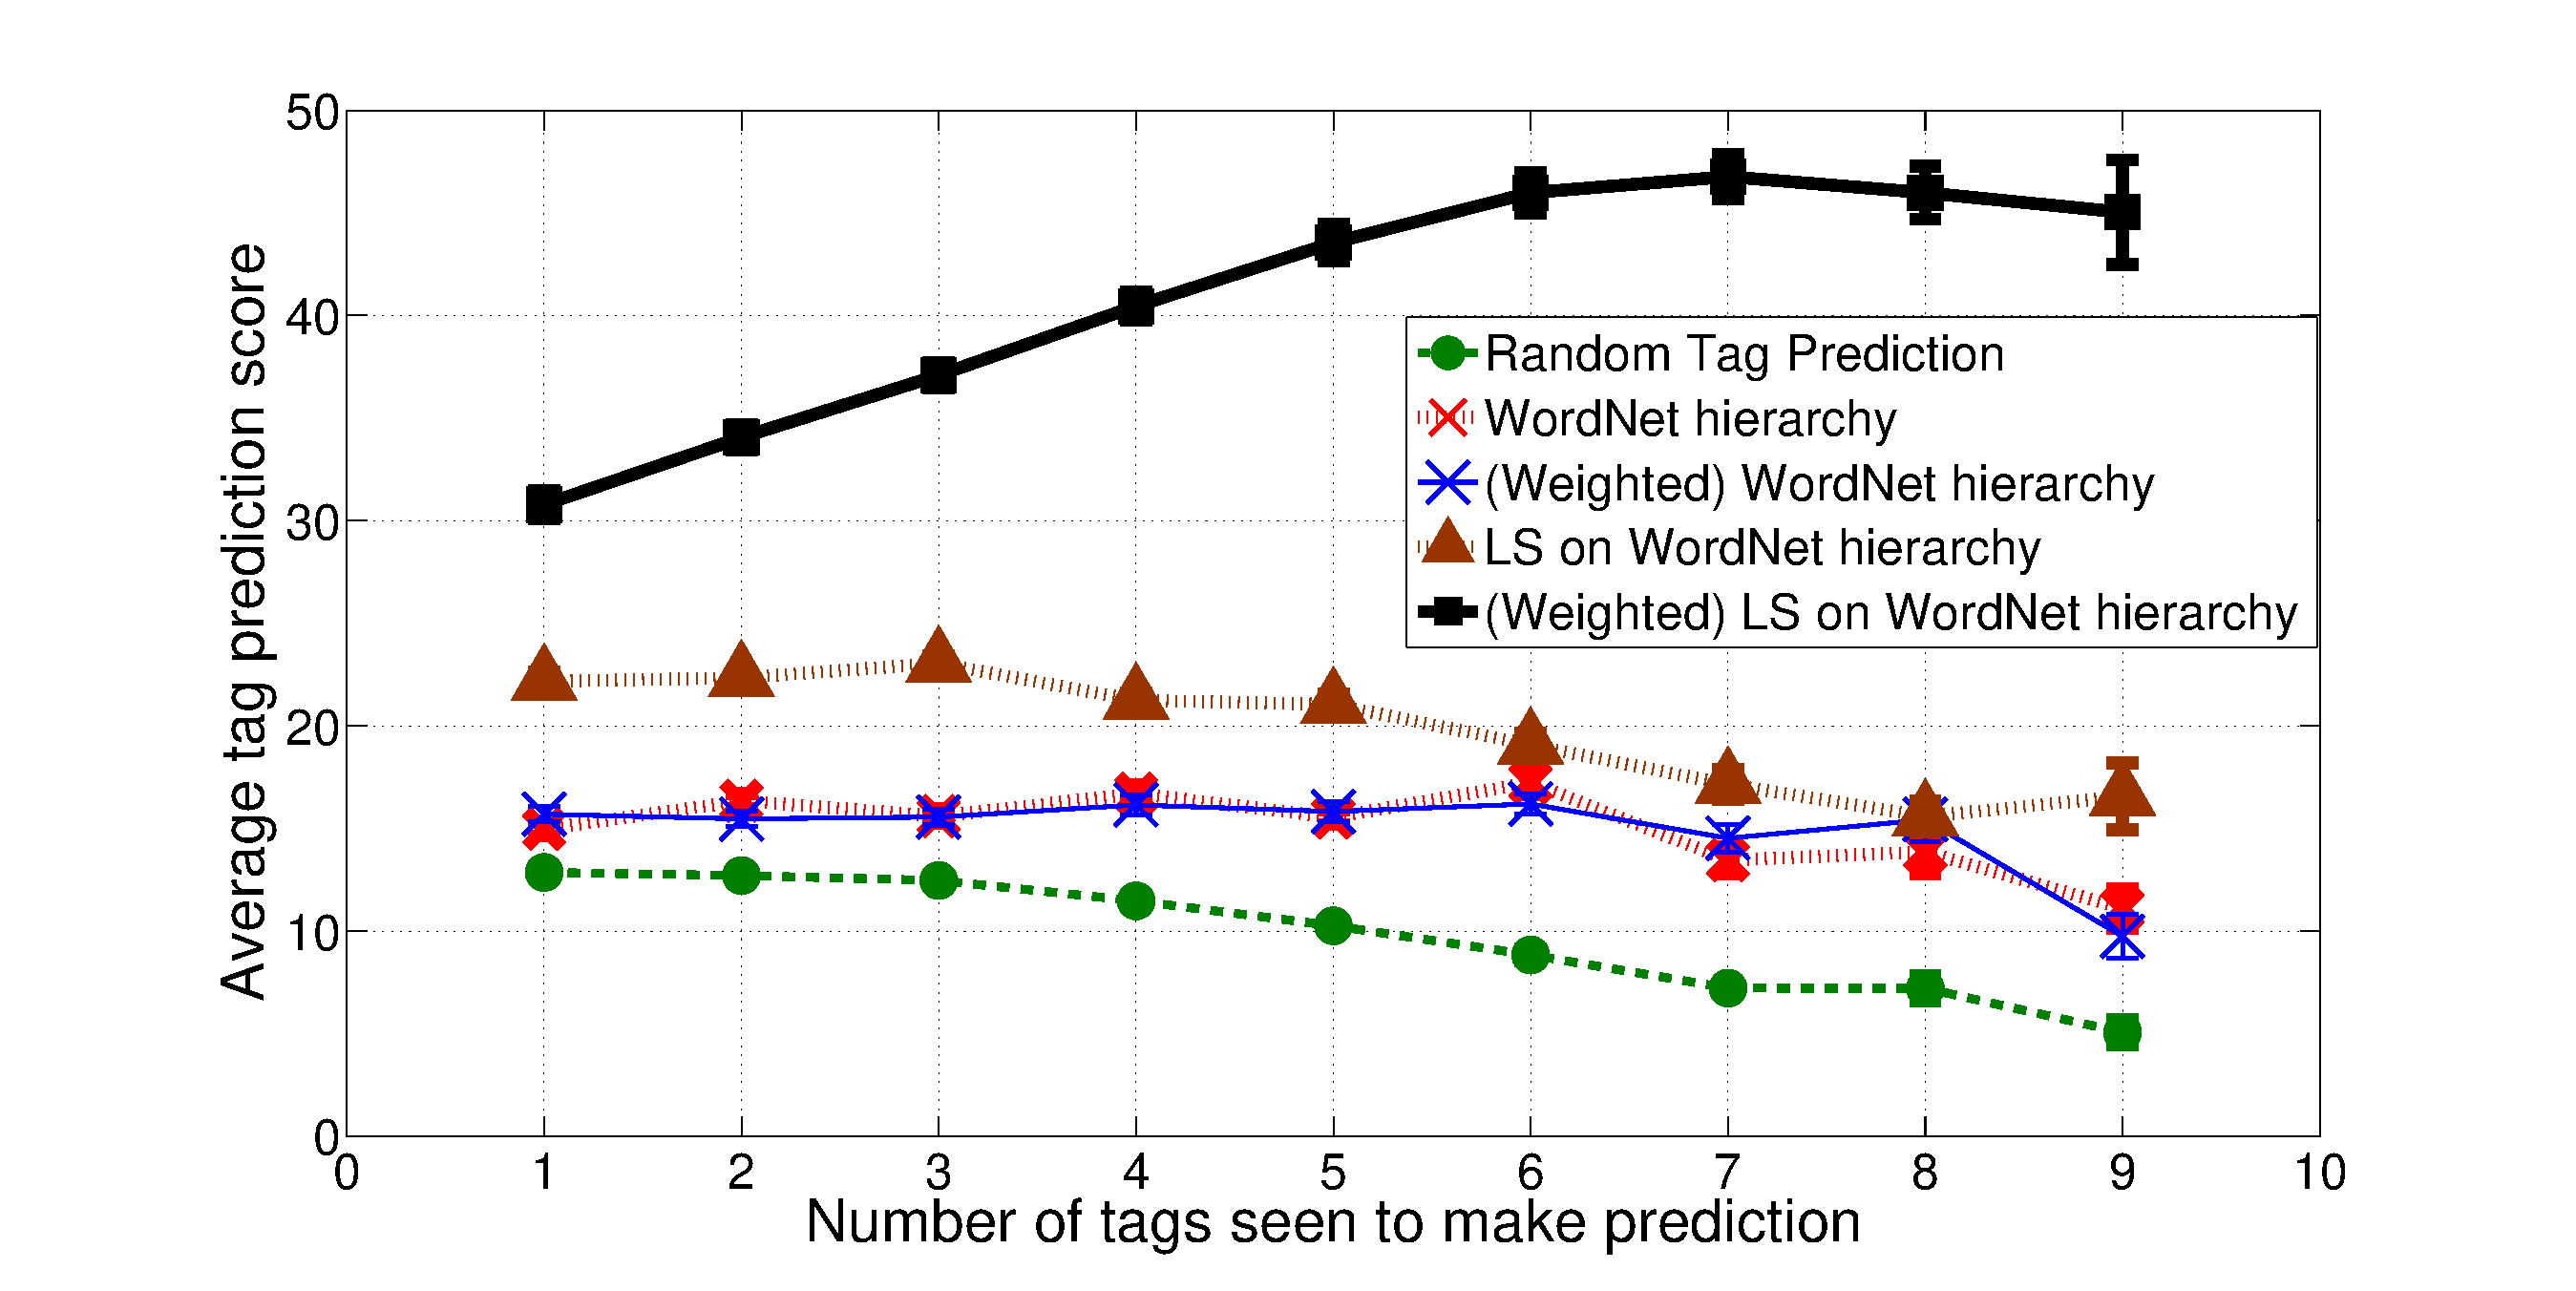
\includegraphics[width=\linewidth]{GWS20TagPredColumnMeanResultsForST}
%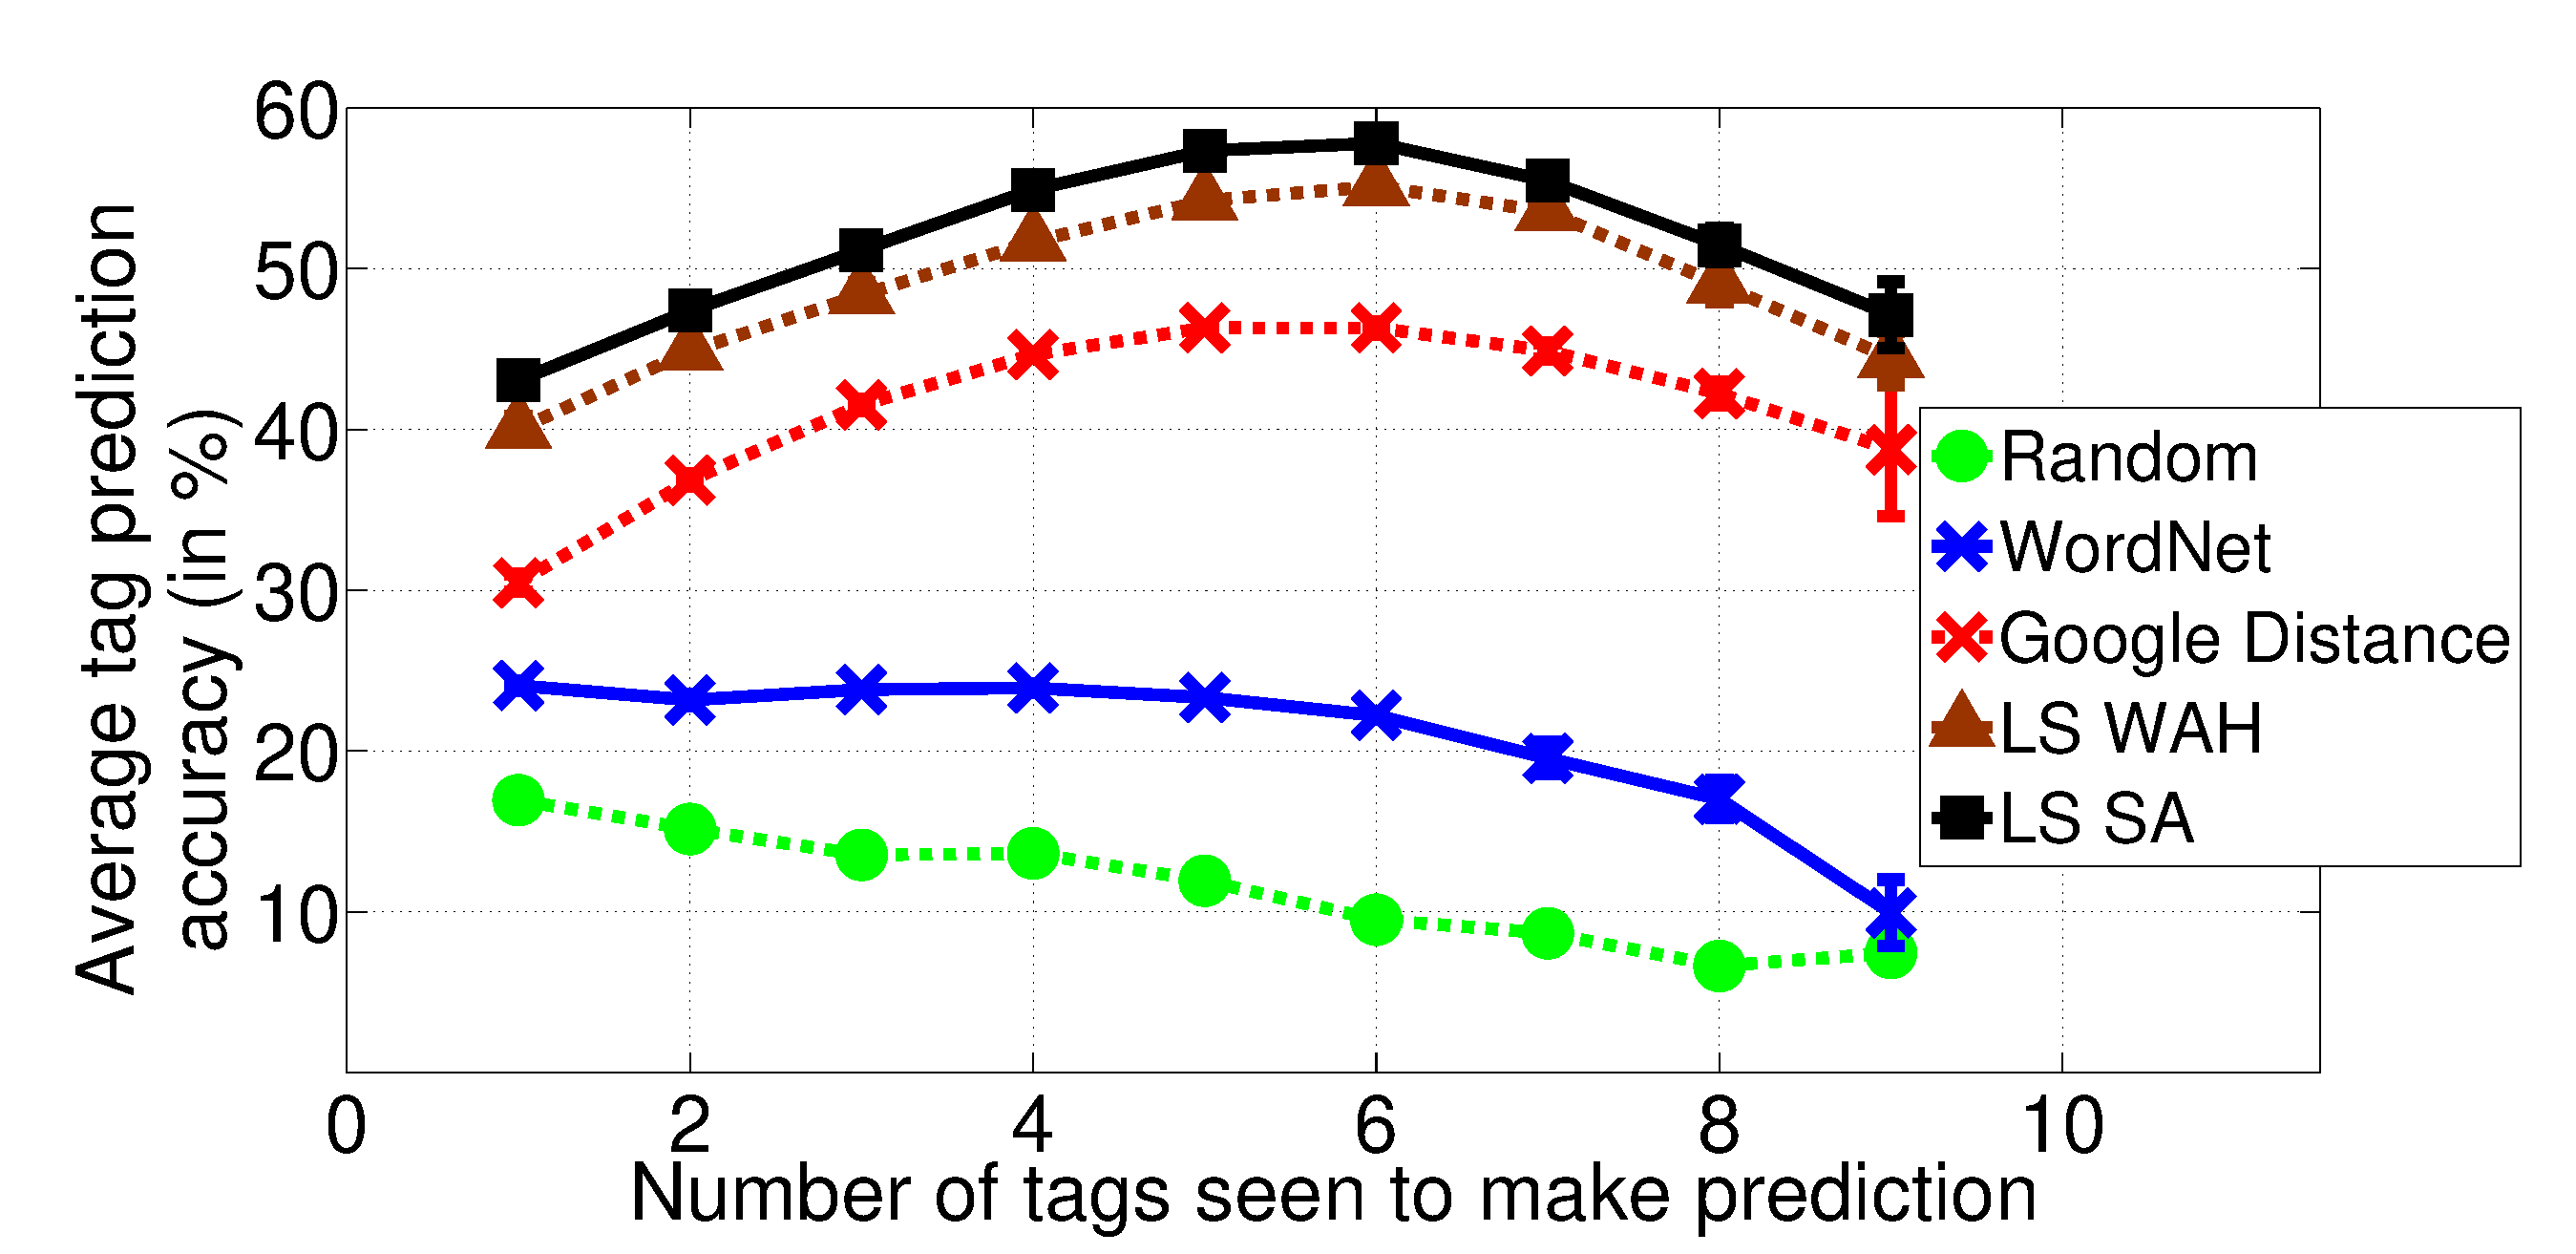
\includegraphics[width=\linewidth]{GWS30_tagPredFig_Journal}
\centering
\includegraphics[width=0.65\linewidth]{TagTree/RebuttalGWS_TP}
\caption{\hl{Average Tag Prediction Accuracies marginalized over $N_{Tags}$ for various methods for the tag prediction task on Stock images corpus.}}
\label{fig:GWS30TagPredGraph}
\end{figure}
\begin{table}[!htbp]
\fontsize{8pt}{1em}\selectfont
\begin{center}
\caption{Average Tag Prediction Accuracies (in \%) obtained using Random method on Stock images corpus.}
\label{tab:TPGWS30Random}
\begin{tabular}{|p{1.5cm}|p{0.5cm}|p{0.5cm}|p{0.5cm}|p{0.5cm}|p{0.5cm}|p{0.5cm}|p{0.5cm}|p{0.5cm}|p{0.5cm}|}
		\hline
		{$\boldsymbol{N_{Seen} \rightarrow}$} & &  &  &  & &  &  &  &\\ 
		{$\boldsymbol{N_{Tags}} \downarrow $} & \textbf{1} & \textbf{2} & \textbf{3} & \textbf{4} & \textbf{5}  & \textbf{6} & \textbf{7} & \textbf{8} & \textbf{9} \\ 
		\hline 		
		\textbf{2} & 1&-&-&-&-&-&-&-&- \\
		\hline
		\textbf{3} & 7&5.28&-&-&-&-&-&-&- \\
		\hline
		\textbf{4} & 11.3&5.8&4.9&-&-&-&-&-&-\\
		\hline
		\textbf{5} & 14.9&10.1&6.8&6.1&-&-&-&-&- \\
		\hline
		\textbf{6} & 19.1&12.9&10.1&9.5&3.1&-&-&-&- \\
		\hline
		\textbf{7} & 21.5&16.1&14.6&10.1&13.1&2.5&-&-&- \\ 
		\hline
		\textbf{8} & 20.7&17.8&11.8&12.7&6.4&9.6&2.3&-&- \\
		\hline
		\textbf{9} & 28.6&25.5&23&19.8&19.4&12.4&7&5.7&- \\ 
		\hline
		\textbf{10} & 28.3&27.6&23.5&23.5&17.7&13.6&16.7&7.6&7.4 \\ 
		\hline
\end{tabular}
\vspace{-2.5mm}
\end{center}
\end{table}
%It is clear that the tag trees built using the proposed approach outperform the baseline graphs constructed using WordNet for all values of $N_{Seen}$. 
%The detailed tables containing Average Tag Prediction Scores for all values of $N_{Tags}$ and $N_{Seen}$ are omitted for brevity but the trend is similar to the one observed for the Flickr corpus.
%\vspace{-5mm}
% The tag prediction score is higher when edge weights of constructed semantic graph are taken as Jaccard similarities between connecting tags. Readers should note however that the improvement is not entirely because of edge weights being Jaccard similarities. Rather, the edges in semantic graph obtain by proposed approach captures corpus specific information in a much more effective manner than semantics-based graphs such as obtained from WordNet. This can be verified by the consistent gap in performance for edge weights being 1, and Jaccard similarities. 
\begin{table}[!htbp]
\fontsize{8pt}{1em}\selectfont
\begin{center}
\caption{Average Tag Prediction Accuracies (in \%) obtained using WordNet method on Stock images corpus.}
\label{tab:TPGWS30Wordnet}
\begin{tabular}{|p{1.5cm}|p{0.5cm}|p{0.5cm}|p{0.5cm}|p{0.5cm}|p{0.5cm}|p{0.5cm}|p{0.5cm}|p{0.5cm}|p{0.5cm}|}
		\hline
		{$\boldsymbol{N_{Seen} \rightarrow}$} & &  &  &  & &  &  &  &\\ 
		{$\boldsymbol{N_{Tags}}\downarrow $} & \textbf{1} & \textbf{2} & \textbf{3} & \textbf{4} & \textbf{5}  & \textbf{6} & \textbf{7} & \textbf{8} & \textbf{9} \\ 
		\hline 		
		\textbf{2} & 1.9&-&-&-&-&-&-&-&- \\
		\hline
		\textbf{3} & 8.9&3.3&-&-&-&-&-&-&- \\
		\hline
		\textbf{4} & 14.2&10.9&3.4&-&-&-&-&-&- \\
		\hline
		\textbf{5} & 21.3&16.9&14.7&8.5&-&-&-&-&- \\
		\hline
		\textbf{6} & 28.4&22.8&22&16.7&9.8&-&-&-&- \\
		\hline
		\textbf{7} & 32.3&28.4&28.4&24.8&22.4&12.6&-&-&- \\
		\hline
		\textbf{8} & 35.7&33.3&32.7&30.7&27.6&23.8&13&-&- \\
		\hline
		\textbf{9} & 36.5&34.5&32.7&31.9&28.7&26.3&23.4&15.5&- \\
		\hline
		\textbf{10} & 37.4&35.2&32.9&30.8&28&26.1&22.3&18.5&9.9 \\
		\hline
\end{tabular}
\vspace{-2.5mm}
\end{center}
\end{table}
\begin{table}[~htp]
\fontsize{8pt}{1em}\selectfont
\begin{center}
\caption{Average Tag Prediction Accuracies (in \%) obtained using Google Similarity Distance method on Stock images corpus.}
\label{tab:TPGWS30Google}
\begin{tabular}{|p{1.5cm}|p{0.5cm}|p{0.5cm}|p{0.5cm}|p{0.5cm}|p{0.5cm}|p{0.5cm}|p{0.5cm}|p{0.5cm}|p{0.5cm}|}
		\hline
		{$\boldsymbol{N_{Seen} \rightarrow}$} & &  &  &  & &  &  &  &\\ 
		{$\boldsymbol{N_{Tags}}\downarrow $} & \textbf{1} & \textbf{2} & \textbf{3} & \textbf{4} & \textbf{5}  & \textbf{6} & \textbf{7} & \textbf{8} & \textbf{9} \\ 
		\hline 		
		\textbf{2} & 3.5&-&-&-&-&-&-&-&- \\
		\hline
		\textbf{3} & 11.2&8.4&-&-&-&-&-&-&- \\
		\hline
		\textbf{4} & 24&26.6&21.9&-&-&-&-&-&- \\
		\hline
		\textbf{5} & 32.3&39.8&39.7&35.2&-&-&-&-&- \\
		\hline
		\textbf{6} & 36.6&43.9&46.5&46.5&44.5&-&-&-&- \\
		\hline
		\textbf{7} & 39.4&44.8&47.8&49.5&49.5&48.5&-&-&- \\
		\hline
		\textbf{8} & 43.6&45.2&47.3&48.5&49.1&49&48.7&-&- \\
		\hline
		\textbf{9} & 41.9&43.5&44.4&45.4&45.9&45.8&45.2&44.9&- \\
		\hline
		\textbf{10} & 41.6&42.7&43.2&42.8&42.6&42&40.7&39.5&38.7 \\
		\hline
\end{tabular}
\vspace{-2.5mm}
\end{center}
\end{table}
\begin{table}[!htp]
\fontsize{8pt}{1em}\selectfont
\begin{center}
\caption{Average Tag Prediction Accuracies (in \%) obtained using LS-WAH method on Stock images corpus.}
\label{tab:TPGWS30LSWAH}
\begin{tabular}{|p{1.5cm}|p{0.5cm}|p{0.5cm}|p{0.5cm}|p{0.5cm}|p{0.5cm}|p{0.5cm}|p{0.5cm}|p{0.5cm}|p{0.5cm}|}
		\hline
		{$\boldsymbol{N_{Seen} \rightarrow}$} & &  &  &  & &  &  &  &\\ 
		{$\boldsymbol{N_{Tags}}\downarrow $} & \textbf{1} & \textbf{2} & \textbf{3} & \textbf{4} & \textbf{5}  & \textbf{6} & \textbf{7} & \textbf{8} & \textbf{9} \\ 
		\hline 		
		\textbf{2} & 7.8&-&-&-&-&-&-&-&- \\
		\hline
		\textbf{3} & 14.6&15.4&-&-&-&-&-&-&- \\
		\hline
		\textbf{4} & 20.5&22.6&22&-&-&-&-&-&- \\
		\hline
		\textbf{5} & 36.2&33.2&32.8&31.3&-&-&-&-&- \\
		\hline
		\textbf{6} & 49&47.6&45.2&43.3&41.5&-&-&-&- \\
		\hline
		\textbf{7} & 59.6&59.4&58.7&57.1&54.4&51.4&-&-&- \\
		\hline
		\textbf{8} & 62.3&63.5&63.2&62.8&61.4&58.2&54.9&-&- \\
		\hline
		\textbf{9} & 56.6&59.7&59.2&58.7&57.9&56.3&52.8&49.5&- \\
		\hline
		\textbf{10} & 53.5&57.6&57.4&56.8&56.1&54.7&52.9&48.5&44.4 \\
		\hline
\end{tabular}
\vspace{-2.5mm}
\end{center}
\end{table}
\begin{table}[!htp]
\fontsize{8pt}{1em}\selectfont
\begin{center}
\caption{Average Tag Prediction Accuracies (in \%) obtained using LS-SA method on Stock images corpus.}
\label{tab:TPGWS30LSSA}
\begin{tabular}{|p{1.5cm}|p{0.5cm}|p{0.5cm}|p{0.5cm}|p{0.5cm}|p{0.5cm}|p{0.5cm}|p{0.5cm}|p{0.5cm}|p{0.5cm}|}
		\hline
		{$\boldsymbol{N_{Seen} \rightarrow}$} & &  &  &  & &  &  &  &\\ 
		{$\boldsymbol{N_{Tags}}\downarrow $} & \textbf{1} & \textbf{2} & \textbf{3} & \textbf{4} & \textbf{5}  & \textbf{6} & \textbf{7} & \textbf{8} & \textbf{9} \\ 
		\hline 		
		\textbf{2} & 7.2&-&-&-&-&-&-&-&- \\
		\hline
		\textbf{3} & 13.4&11.1&-&-&-&-&-&-&- \\ 
		\hline
		\textbf{4} & 28.4&27&21.1&-&-&-&-&-&- \\
		\hline
		\textbf{5} & 44.5&41.9&38.5&35&-&-&-&-&- \\
		\hline
		\textbf{6} & 53.3&53.3&51.3&49.5&46.9&-&-&-&- \\
		\hline
		\textbf{7} & 61.7&63.2&62.6&60.8&58.3&56&-&-&- \\
		\hline
		\textbf{8} & 64.3&64.8&65.8&65.3&63.1&60.2&57.4&-&- \\
		\hline
		\textbf{9} & 59&60.2&60.8&61.1&60.8&58&55.3&52.3&- \\
		\hline
		\textbf{10} & 55.7&57.7&57.9&57.8&57.6&57&53.7&50.6&47.1 \\
		\hline
\end{tabular}
\vspace{-2.5mm}
\end{center}
\end{table}

\begin{table}[!htp]
\fontsize{8pt}{1em}\selectfont
\begin{center}
\caption{\hl{Average Tag Prediction Accuracies (in \%) obtained using the Symmetric sum approach on Stock images corpus.}}
\label{tab:TPGWS30Jij}
\begin{tabular}{|p{1.5cm}|p{0.5cm}|p{0.5cm}|p{0.5cm}|p{0.5cm}|p{0.5cm}|p{0.5cm}|p{0.5cm}|p{0.5cm}|p{0.5cm}|}
		\hline
		{$\boldsymbol{N_{Seen} \rightarrow}$} & &  &  &  & &  &  &  &\\ 
		{$\boldsymbol{N_{Tags}}\downarrow $} & \textbf{1} & \textbf{2} & \textbf{3} & \textbf{4} & \textbf{5}  & \textbf{6} & \textbf{7} & \textbf{8} & \textbf{9} \\ 
		\hline 		
		\textbf{2} & \hl{11.1} & -  & -  & -  & -  & -  & -  & -  & - \\
		\hline
		\textbf{3} & 16.9 & 17.7 & -  & -  & -  & -  & -  & -  & -\\ 
		\hline
		\textbf{4} & 32.1 & 32.5 & 29.7 & -  & -  & -  & -  & -  & - \\
		\hline
		\textbf{5} & 45.1 & 47.8 & 46.4 & 43.1 & -  & -  & -  & -  & - \\
		\hline
		\textbf{6} & 52.7 & 56 & 56.3 & 55.5 & 53.2 & -  & -  & -  & - \\
		\hline
		\textbf{7} & 62.1 & 64.6 & 64.9 & 63.9 & 62 & 59.9 & -  & -  & - \\
		\hline
		\textbf{8} & 64.5 & 68 & 68.1 & 67.8 & 65.8 & 63.1 & 60.5 & -  & - \\
		\hline
		\textbf{9} & 60.6 & 63.9 & 64.9 & 64.9 & 64 & 61.5 & 58.5 & 55.9 & - \\
		\hline
		\textbf{10} & 58 & 61.5 & 62.9 & 63.2 & 63.1 & 61.6 & 58.9 & 55 & \hl{52.3}\\
		\hline
\end{tabular}
\vspace{-2.5mm}
\end{center}
\end{table}


\indent The results indicates that the proposed local search paradigm based approach has successfully adapted the ontological tag tree obtained from WordNet to the Flickr or stock images corpus. \hl{We can obtain performance better than or close to that of other tag prediction approaches, while having several orders of savings in the space requirement. } We next describe the second data-driven task used for evaluation of tag trees. 
\subsection{Efficient Classification Task}
\label{sec:effClassification}
\hl{We consider the problem of efficiently associating tags with resources based on the resource content. For domains where it is feasible to extract features from the resource and to train concept detectors, we show how tag trees can be utilized to determine which concept detectors should be applied on a given test resource. We demonstrate this using annotated image corpora and utilize different modalities to represent the content of a given resource. }
Given a test image, $i$ from the corpus without any associated tags or keywords, we predict which of the $N$ tags are applicable to the image. By letting each of the $N$ tags correspond to a category or class, this is equivalent to a multi-class, multi-label classification task. Let us assume that one-vs-all binary classifiers are available for each tag class - these take the image instance $i$ as input and can predict $P(j \mid i)$ where class $j$ corresponds to tag $t_j$. We can use this to predict whether or not a tag $t_j$ should be associated with image $i$ based on whether $P(j \mid i)$ is greater than an appropriate threshold $\theta$ or not. 

The naive approach to predict all tags applicable to $i$ would be to test each of the $N$ classifiers on $i$ and accumulate those tags for which the predictions by the corresponding classifiers exceed $\theta$. \hl{Some works such as {\cite{li2013classifying}} propose techniques to make classification of images faster. However in order to do this, these works require re-training of classifiers and cannot utilize existing classifiers for each tag. 
%For example {\cite{li2013classifying}} proposes an approach to select positive and negative examples determined most relevant with respect to a given concept. 
Contrary to these, in the proposed approach, we can utilize pre-trained classifiers corresponding to different tags. Other works such as the image annotation application in {\cite{wu2008flickr}} associate a test image with tags based on applying all concept detectors on the test image and then combining the predictions. However such approaches require applying all $N$ classifiers to a given test image and are hence inefficient for a large number of tags. }
This process can be made more efficient by using the ontological tag tree on the set of tags. Once certain labels have been predicted for an image $i$, one can utilize the tree structure to decide which tags are more or less likely to be associated with the image. Thus the choice of the classifiers to test next on the image $i$, can be made in a more efficient manner.  Therefore, a tag tree that captures the relations between the tags more effectively, is expected to lead to more efficient performance by reaching the correct number of predicted tags with fewer number of binary classifications performed. The \emph{efficient classification task} is formulated to measure the classification efficiency in such a setting. 

\indent This evaluation task is formulated as follows. Given $N$ binary classifiers, the $j^{th}$ classifier predicts probability $P(j \mid i)$ of tag $t_j$ being associated with a test image $i$. $K$ binary classifications are performed for image $i$ and the set of tags that are predicted positive among those $K$ classifications, comprise the set of predicted tags $\mathbb{P}_{i,K}$ for image $i$ for given $K$. The ground truth set of tags that are associated with image $i$ as per the corpus, is denoted $\mathcal{T}_{i}$. We define performance of the classification task based on the Tag Recall as defined below.
%** Check if Recall can be defined like this? Or does it have to be wrt different instances? ** \\
\begin{equation} 
\text{Tag Recall} = \frac{\mid \mathcal{T}_i \cap \mathbb{P}_{i,K} \mid}{ \mid \mathcal{T}_i \mid} 
\label{eq:TagClassfnRecall}
\end{equation} 

Based on the above definition, the Tag Recall is monotonically increasing with $K$: as more than $K$ classifications are performed, the cardinality of the set of predicted labels can remain constant or increase, leading to a non-decreasing value for the Tag Recall. 

%\subsection{Baseline Methods}
%\label{subsec:baselines}
\indent The most naive way of choosing the order in which the $N$ classifications are performed, would be to choose each binary classifier randomly. A more sophisticated approach can be adopted by choosing the classifiers based on the decreasing order of their class priors in the training corpus, i.e., choosing the classifier corresponding to the most frequently occurring tag first, followed by the next popular tag, and so on. We refer to these methods as Random, and Prior-based respectively. Below we discuss how the classifiers can be chosen based on their priors and a given ontological tag tree. 

\subsubsection{Utilizing Ontological Tag Tree for Classification} 
\label{sec:EffClassifnUsingGraph}
Intuitively, the procedure for using an ontological tag tree to decide how to choose the classifiers, is similar to the approach for the tag prediction task. For image $i$, once certain tags are predicted as present, the tags in their proximity (as per the tag tree) have a higher chance of being present too, and the corresponding classifiers should be tested sooner. Similarly, the predicted absence of tags brings down the chance that tags in their proximity will be present. We define below a priority score for the tags that have not been tested for, based on their priors and the predictions for the tags that have been tested for. For image $i$ and tag tree $T$, we define 
\begin{equation} \label{eq:FastClassifyEqn} 
priority(j) = P_{prior}(j) + \sum_{c \in C_{tested}}  {(P( c \mid i)- \theta) \times  (1-dist'(c, j)) }
%\theta = 1. 
\end{equation}
where $dist'(c,j)$ is the distance $dist(c,j)$ as defined in Section \ref{sec:TagPredUsingGraph} for various methods, normalized with respect to its maximum value such that $dist'(c,j)$ varies between 0 and 1. $P_{prior}(j)$ is the prior probability of tag $t_j$, and $C_{tested}$ is the set of tags that image $i$ has been tested for. Algorithm~\ref{EffClassfnAlgo} utilizes (\ref{eq:FastClassifyEqn}) and presents the algorithm employed to decide the order of classifications for each image $i$. For a given image $i$ and given $K$, the set of labels predicted as present, i.e., $\mathbb{P}_{i,K}$ can be obtained using Algorithm~\ref{EffClassfnAlgo}. \\ 
\begin{algorithm}[!t]
\fontsize{8pt}{1em}\selectfont
\caption{Algorithm for Efficient Classification by using Ontological Tag Tree} 
\label{EffClassfnAlgo} 
\textbf{Input:} \\ 
$\cdot$ $C_j$: classifier for label $j \,$ corresponding to tag $t_j$ ($\forall j \in \mathcal{T} $), that can provide $P(j \mid i)$ for image $i$; threshold $\theta$ \\ 
$\cdot$ $P_{prior}(j)$: prior probability for tag $t_j$  \\
$\cdot$ $dist'(t,t')$: normalized inter-tag distances calculated based on given tag tree as outlined in Section~\ref{sec:EffClassifnUsingGraph}\\
$\cdot$ $K$: number of binary classifications to perform \\ 
\textbf{Initialize:} $L_{tested} $ = [ ]  \\
\textbf{Loop While} $\mid  L_{tested}  \mid$  $ \le \; K$  \\
\hspace*{5mm} $\cdot$ Calculate priority score for all tags in $(\mathcal{T} \setminus L_{tested}  )$ \\
\hspace*{5mm} using (\ref{eq:FastClassifyEqn}) \\
\hspace*{5mm} $\cdot$ Test classifier $C_{\hat{j}}$ corresponding to tag $t_{\hat{j}}$  with highest \\
\hspace*{5mm} calculated priority score to get $P( \hat{j} \mid i)$. \\
\hspace*{5mm} $\cdot$  $L_{tested} = L_{tested} \cup \hat{j}$. \\
\textbf{EndWhile}. \textbf{Output:} $\mathbb{P}_{i,K} = \{ j: P(j \mid i) > \theta , \, \, \,  j \in  L_{tested} \} $ 
\end{algorithm}
\textbf{Flickr corpus:} We use the same set of 117 Flickr tags as described in Section ~\ref{subsec:TagPred}. In order to train image classifiers 500,000 Flickr training images are used. Each tag $t_j$ is treated as a class. Positive training images are those that associated with the corresponding tag $t_j$ and negative training are those that are not. We use a ratio of $1:10$ for number of positive instances to number of negative instances for each class. SIFT features~\cite{lowe} are used to train binary SVM classifiers for each class. We provide results for the Random and Prior-based methods as discussed in Section~\ref{sec:effClassification}, and for methods 2 through 6 described in Section~\ref{sec:comparison} using the approach outlined in Section~\ref{sec:EffClassifnUsingGraph}. For $\theta = 0.5$, the Tag Recall observed with varying number of classifiers tested, i.e., $K$, are shown in Fig.~\ref{fig:EfficientTagPredGraphFlickr}. \hl{Note that {\cite{sigurbjornsson2008flickr}} does not utilize the symmetric similarities for an application as proposed in Section {\ref{sec:effClassification}}, however we utilize the symmetric jaccard similarities as per Algorithm ({\ref{EffClassfnAlgo}}) and compare against our approach for an understanding of the trade-off between performance and space requirement. 
%and compare the performance in order to provide an understanding of the .
 It is clear that for a given $K$, our approach outperforms the tag tree constructed from WordNet, the tag graph using Google Distance, and the ones that select classifiers randomly or solely based on prior. Performance of the LS-SA method is very close to that of the Symmetric sum method despite having several orders of savings in the space requirement as discussed in Sections {\ref{sub_sec:relatedWork}} and {\ref{subsec:TagPred}}}. For Tag Recall of around 4.4\%, the tag tree based on proposed approach (LS-SA) requires only 11 classifications compared to 21 for LS-WAH, 31 for Google Distance based, 51 for WordNet, 36 Prior based, and 61 when the classifiers are randomly selected. These correspond to 91\%, 182\%, 363\%, 227\%, 454\% \textit{additional} classifications used by these methods respectively, compared to the proposed method with Similarity Approximation (LS-SA). The WordNet based method performs worse than the Prior-based method, implying that the using semantics based distance with priors is less efficient than using priors alone. Visual-feature based image classification is a hard problem and the Tag Recall for 117 classes even after all 117 classifiers are tested, is observed to be less than 10\%. This is also a result of the individual classifiers and of the chosen threshold $\theta$. Note that the Tag Recall~(\ref{eq:TagClassfnRecall}) is different from recall of a class. For $\theta=0.5$, when all the classifiers are tested, the average recall over all classes is 10.5\% and the average precision is 15.9\%. \\
\indent A more lenient (i.e., lower) $\theta$ would lead to higher Tag Recall as can be seen in Fig.~\ref{fig:EfficientTagPredGraphFlickrLower}. $\theta=0.3$ corresponds to an average recall of 37.7\% and average precision of 4.9\%. A lower $\theta$ also implies less relative weight given to $P_{Prior}(j)$ in (\ref{eq:FastClassifyEqn}) and as a result, the WordNet method performs worse than even the Random method.  \\ 
\indent \textbf{Stock images corpus:} We perform experiments on the same corpus that was described in Section ~\ref{subsec:TagPred}. \hl{In order to show the applicability of our approach to different modalities that can be used to represent a given resource, we utilize
the textual caption accompanying the image $i$ to represent the image.} A TF-IDF based bag-of-words representation is used for each image, followed by binary SVM classifiers for each class. As in the case of Flickr, we present variation of Tag Recall with $K$ for various methods for $\theta=0.5$ in Fig.~\ref{fig:EfficientTagPredGraphGetty}. $\theta=0.5$ corresponds to an average recall of 73.6\% and average precision of 75.6\%. 
Our approach is seen to be able to better decide which classifiers to test, for a given $K$ and as a result, leads to higher Tag Recall for a fixed $K$. For Tag Recall of around 48\%, the tag tree based on the proposed approach (LS-SA) requires only 7 classifications compared to 9 for LS-WAH, 9 for Google Distance based, 15 for WordNet, 11 for only prior based and 21 when the classifiers are randomly selected. These correspond to 29\%, 29\%, 114\%, 57\%, 200\% \textit{additional} classifications used by these methods respectively, compared to the proposed method with Similarity Approximation (LS-SA).  \\ 
\indent It should be noted that the goodness of predictions i.e., the precision and recall obtained when all classifiers are tested, is essentially a property of the set of classifiers, which are the same for various methods used for this task. Based on the experiments, we have demonstrated that using ontological tag trees constructed through the proposed approach makes selection of classifiers much more efficient as compared to using purely semantics based tag tree or tag graphs built using commonly used techniques. \hl{We have also shown that we can achieve a performance almost as high as other approaches despite having several orders less space requirement. 
}
%conventionally, Tag Recall is reported with precision,  we only provide Tag Recall results since the objective of this task is to predict labels (tags) for given test image $i$ in as less binary classifications as possible. Also, the trade-off between precision and recall is essentially a property of the classifiers which are the same for various methods used for this task. \\
% \subsection{Evaluation of Semantic Graph Through Classification}  
% \label{EvalSemGraphClassifn}
% The caption associated with an image is used to represent it in a text-based bag-of-words representation. We prune words that occur in captions of less than two images, and remove stop words to construct a textual vocabulary of 21543 words. Each image is represented using TF-IDF numbers on the constructed vocabulary. 30 keywords are selected from Getty based on the keywords that were most popular, were not stop words, and occurred in WordNet hierarchy too. Each of the 30 keywords is considered a class for the purpose of evaluation. One-vs-rest Support Vector Machine is used to train a binary classifier for each class that can give probabilistic scores for its predictions. For training, we pick around 1000 images per class that are associated with the corresponding keyword. These comprise the positive instances. It is possible that the picked images are also associated with other keywords but we discard the overlap between classes (keywords) while training in order to avoid introducing any bias in the training set. The negative instances for a class comprises of the positive instances for other classes. For the testing set we collect around 1000 images per class and note all keywords associated with each testing image.  \\ 
% \indent \textit{Utilizing Semantic Graph for Classification} - Given is a semantic graph where each node $i$ corresponds to a class $i$. While training binary classifier for class $i$, we weigh the negative instances depending on their position in the semantic graph, with respect to the node $i$. Specifically, the instances of class $j$ are given a weight of $w_{i,j}$ while training binary classifier for class $i$ where\\
% \begin{math} 
% w_{i,j}=\frac{\text{Number of hops between $i$ and $j$}}{\text{Maximum number of hops between $i$ and any other node}}.
% \end{math}
% Given a test instance, the class with highest posterior probability is th predicted label. Accuracy is measured as 100\% if the predicted class (keyword) for a test image is associated with the test image,  and 0\% otherwise. \\ 
% \\
% \begin{figure}[ht!]
% \centering
% \includegraphics[width=3.7in]{cmcAccuracyClassifiersGaurav.eps}
% \caption{Classification accuracy obtained by utilizing various semantic graphs}
% \label{fig:ClassifierAccuracyGraph}
% \end{figure}
% Figure ~\ref{fig:ClassifierAccuracyGraph} shows how the classification accuracy varies with number of keywords predicted (K) for each test image. The accuracy increases with K since it is measured by whether even one predicted label is associated with the test instance. Our local search based approach is seen to outperform WordNet in terms of classification accuracy. 
\begin{figure}[!htp]
%\epsfig{width=10cm,figure=FastTagPredFWS117topK.eps}
%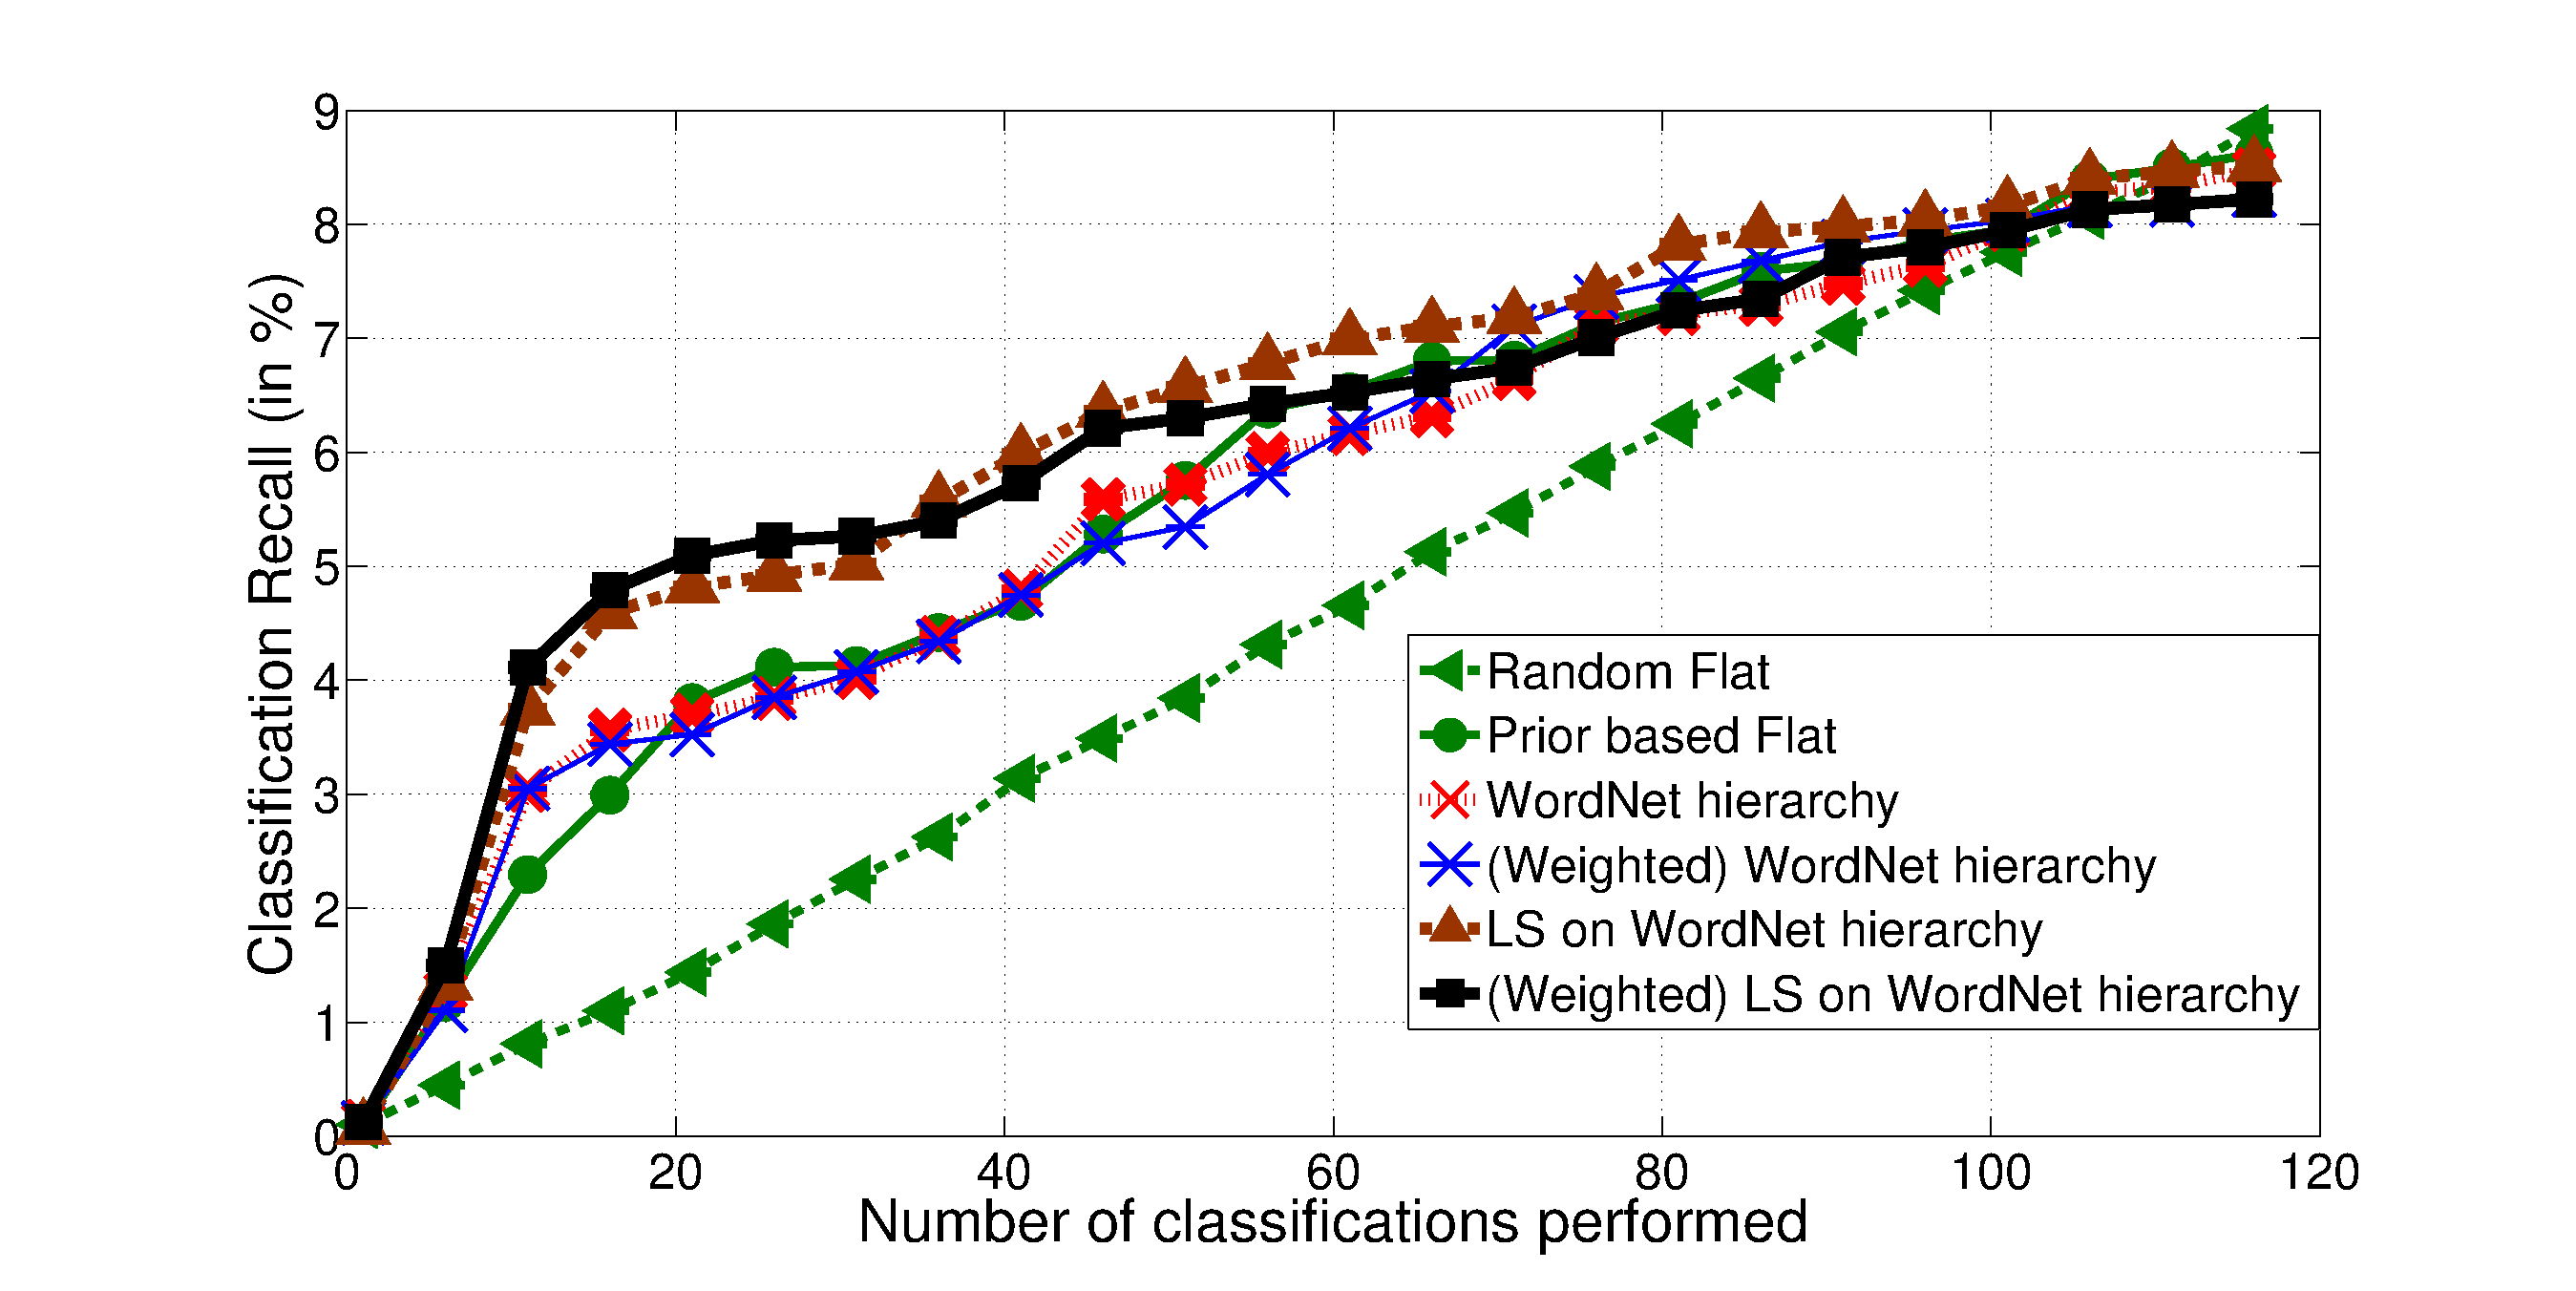
\includegraphics[width=\linewidth]{FastTagPredFWS117topK}
%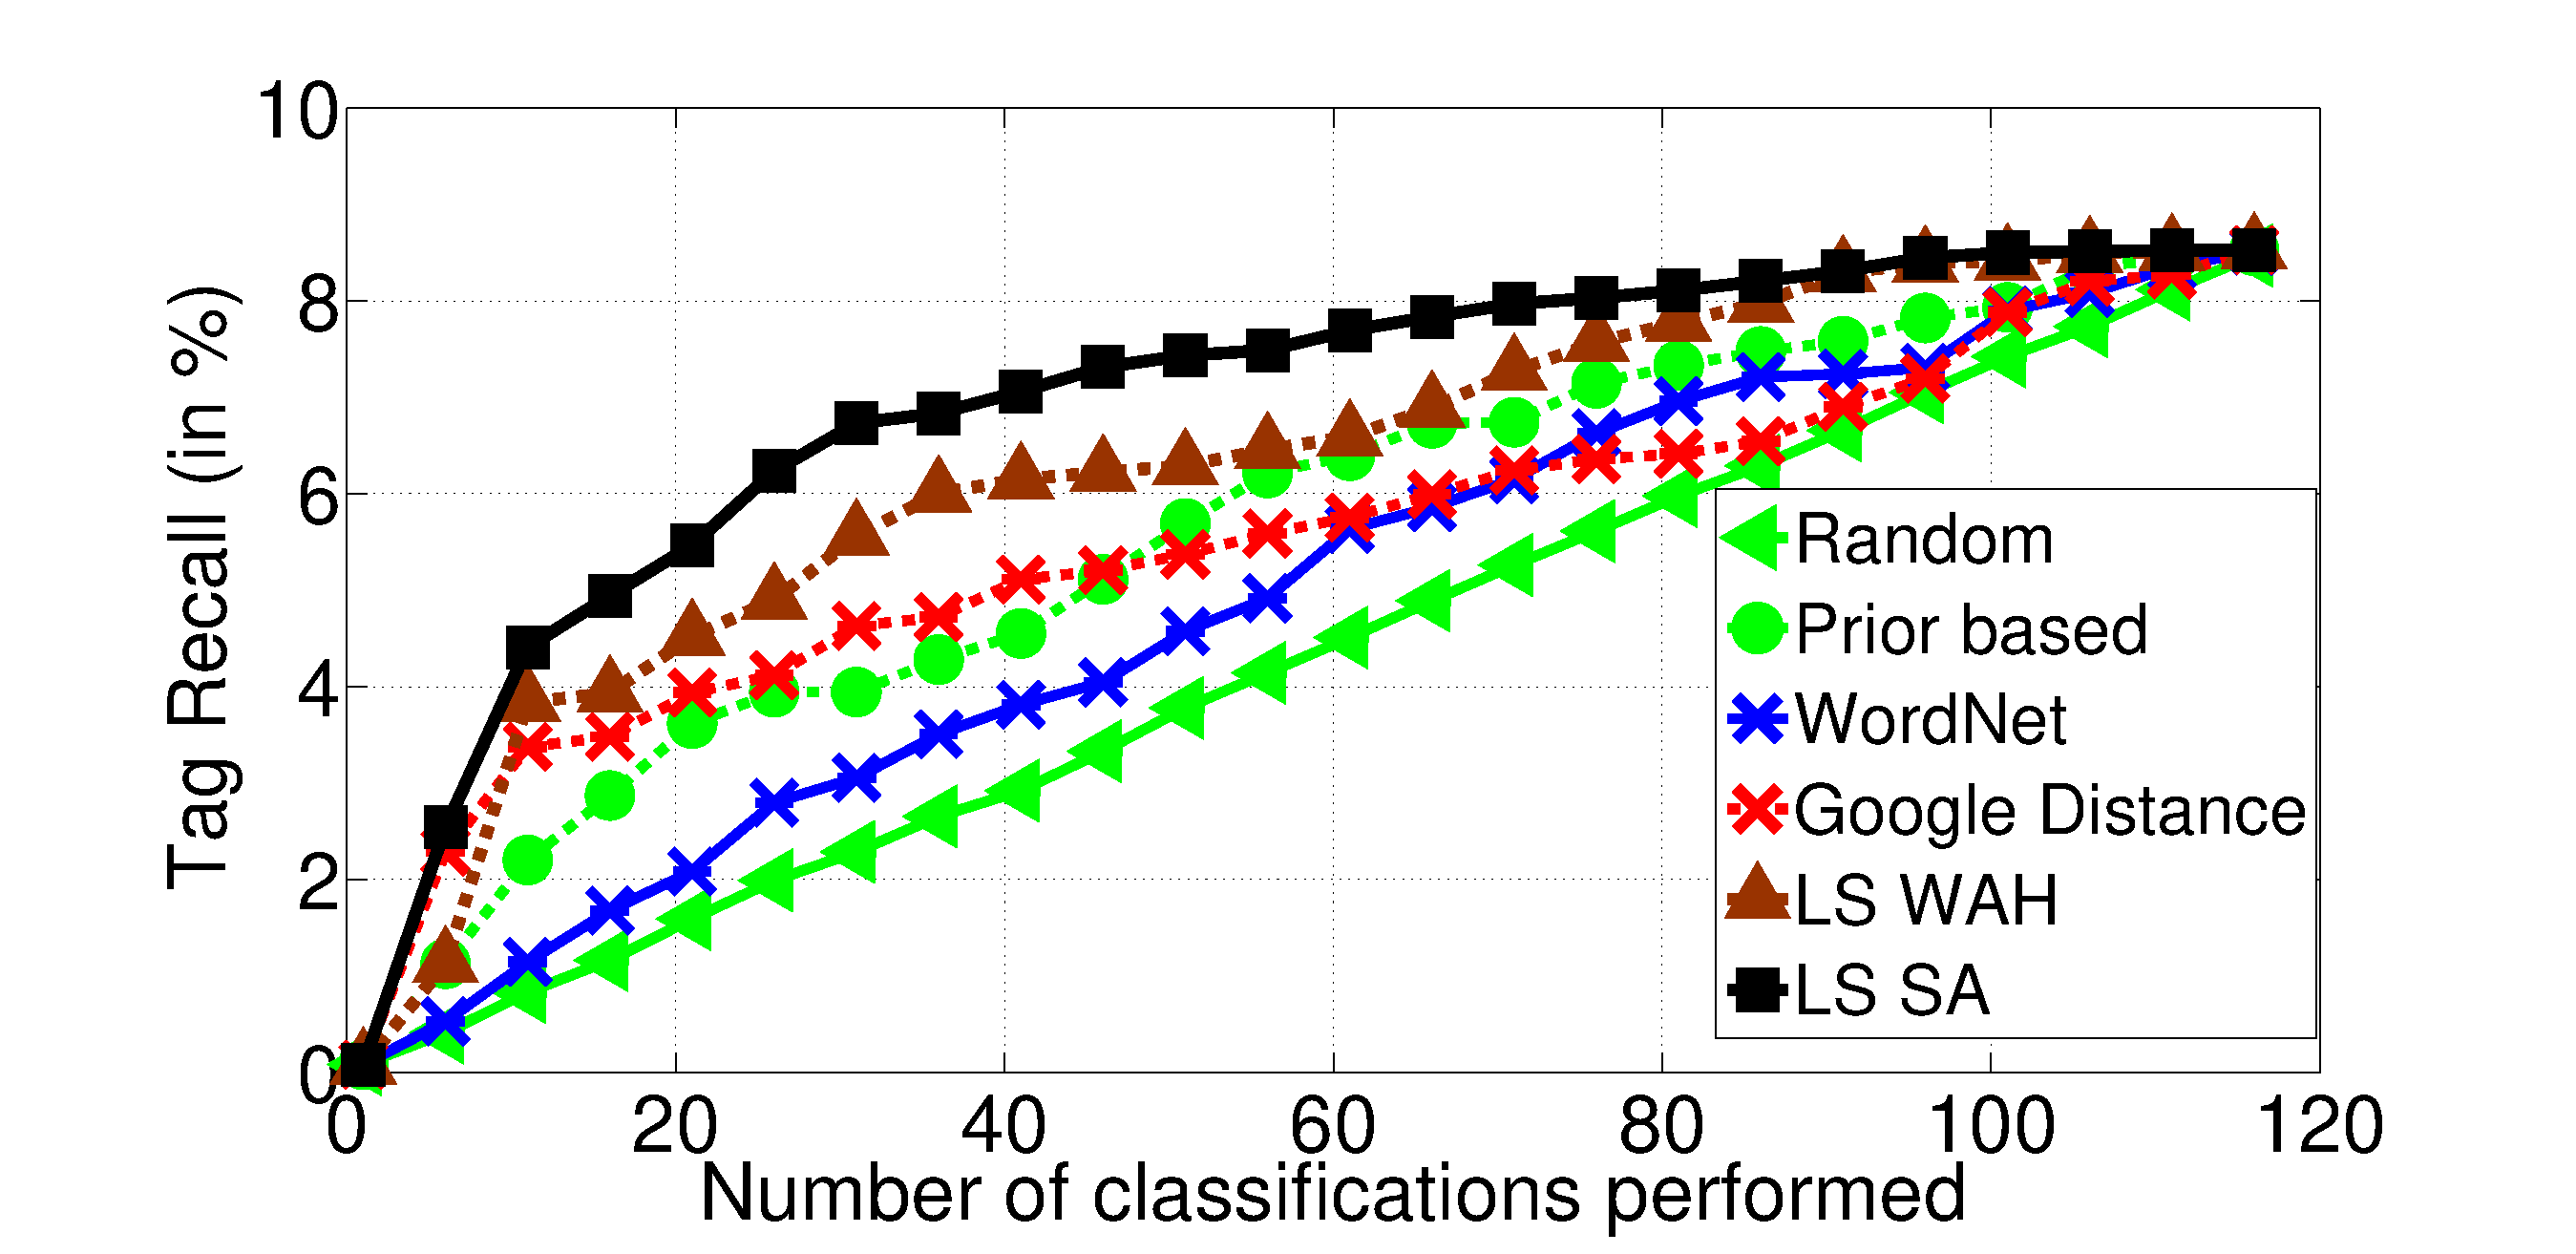
\includegraphics[width=\linewidth]{FWSFastTP_journal.eps}
\centering
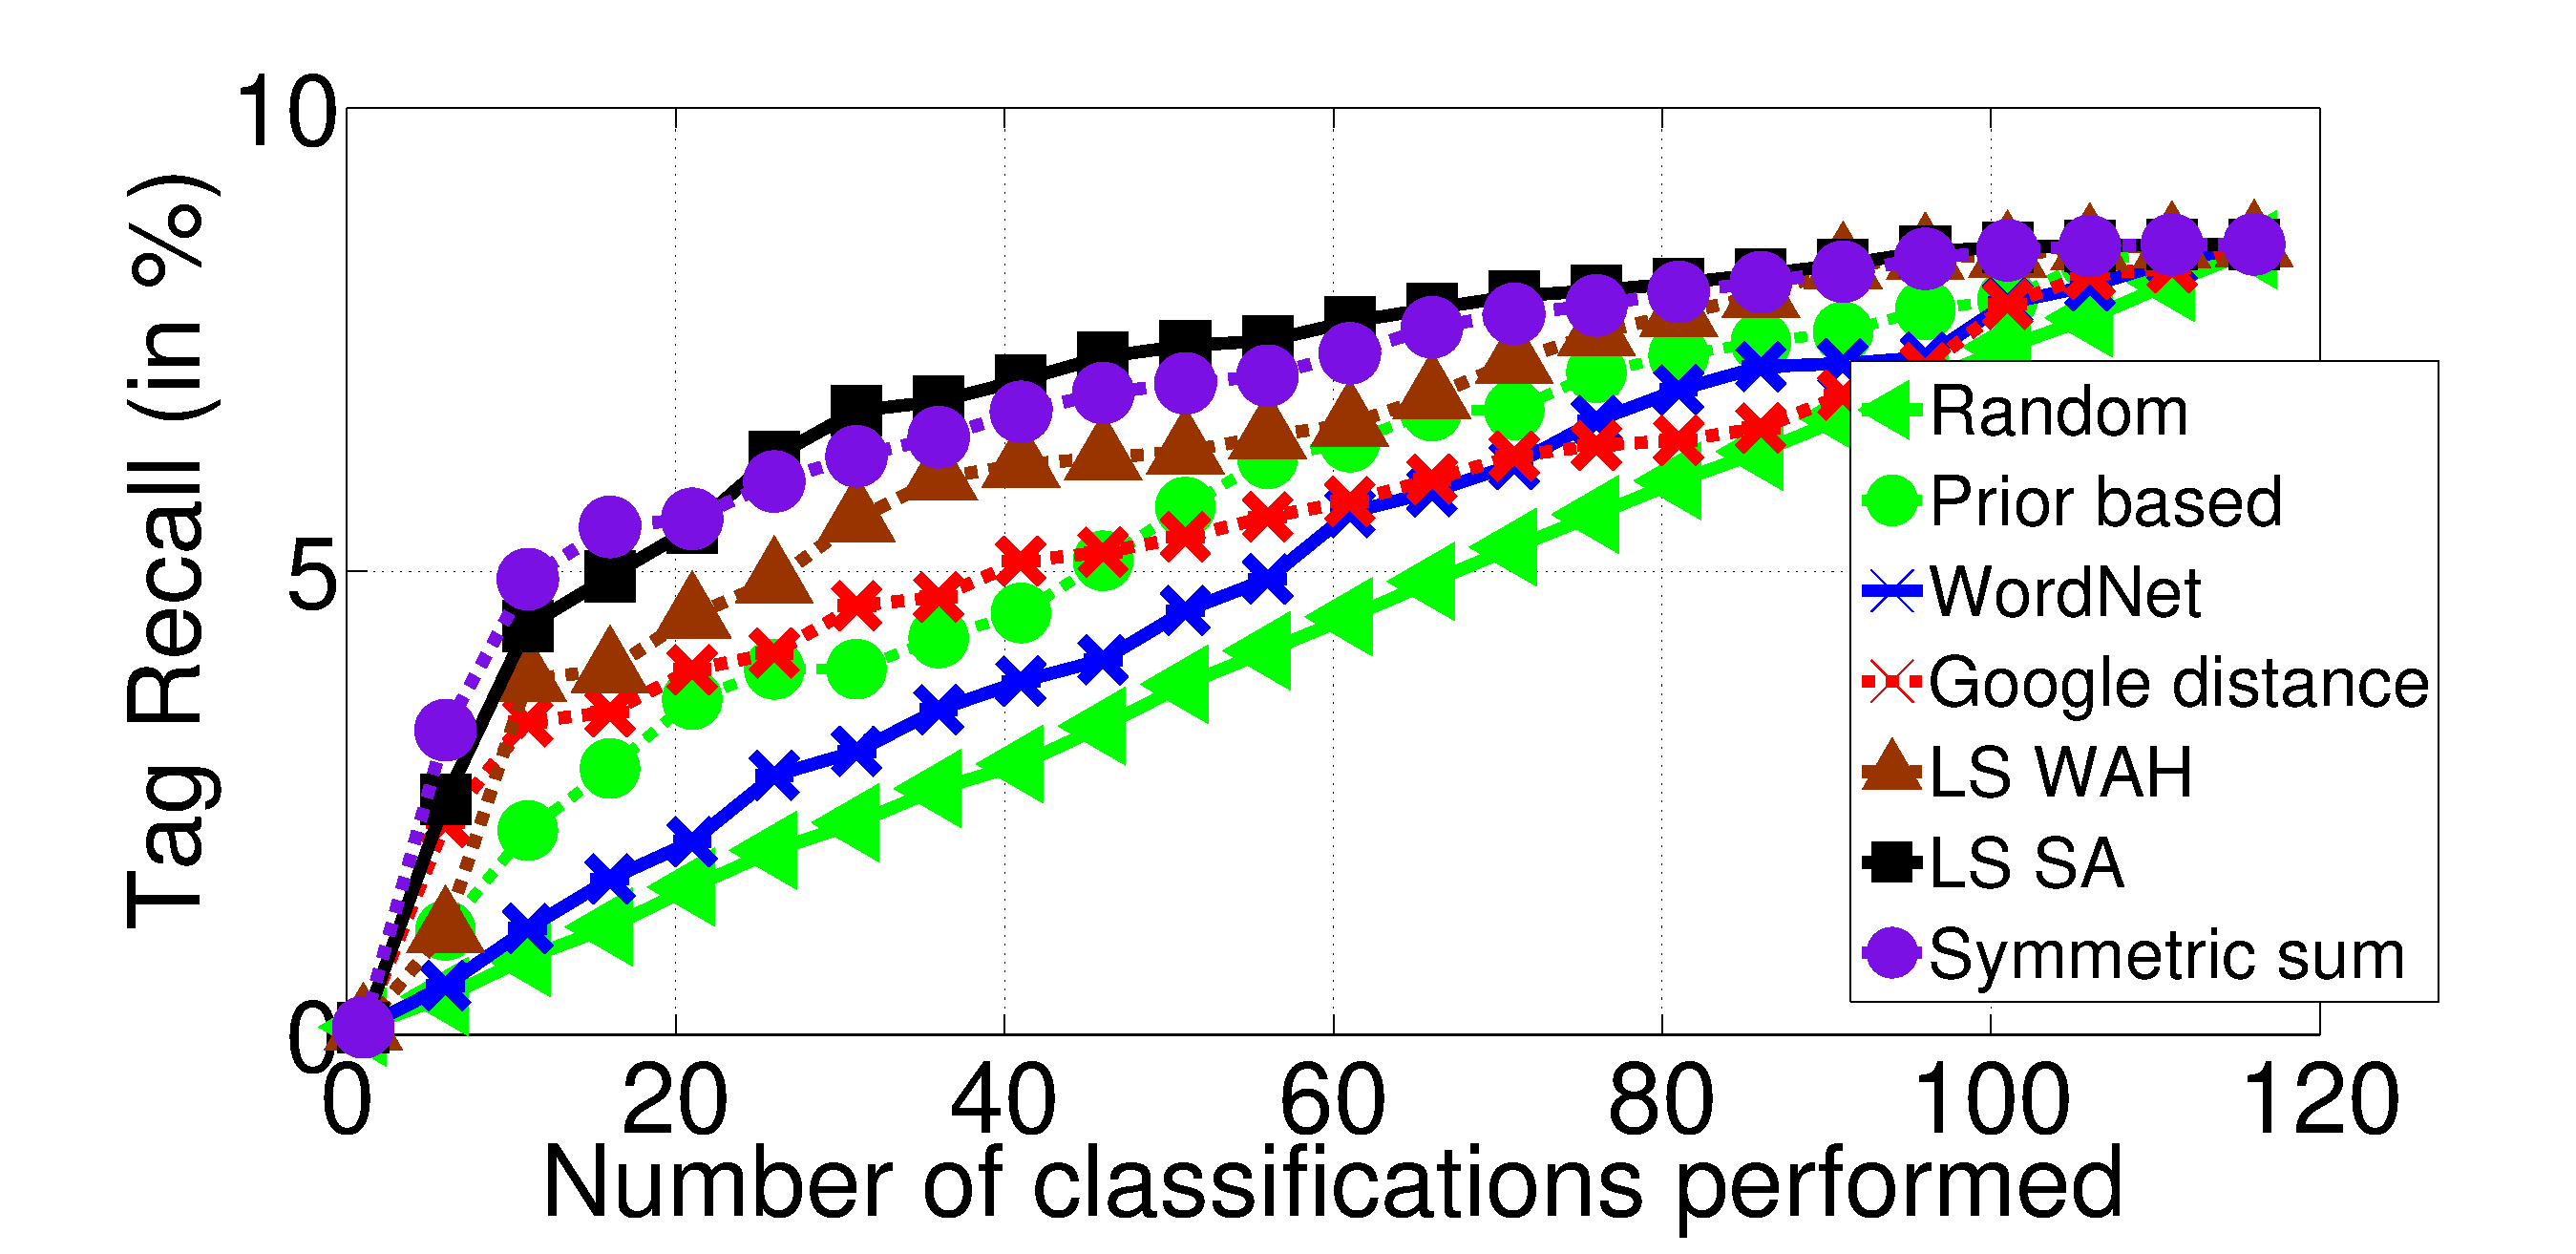
\includegraphics[width=0.65\linewidth]{TagTree/RebuttalFlickrFastTP}
\caption{\hl{Tag Recall obtained with respect to number of classifications performed for Flickr corpus. $\theta$ is chosen to  be 0.5.} } 
\label{fig:EfficientTagPredGraphFlickr}
\end{figure}
\begin{figure}[!htp]
%\epsfig{width=10cm,figure=FastTagPredFWS117topK.eps}
%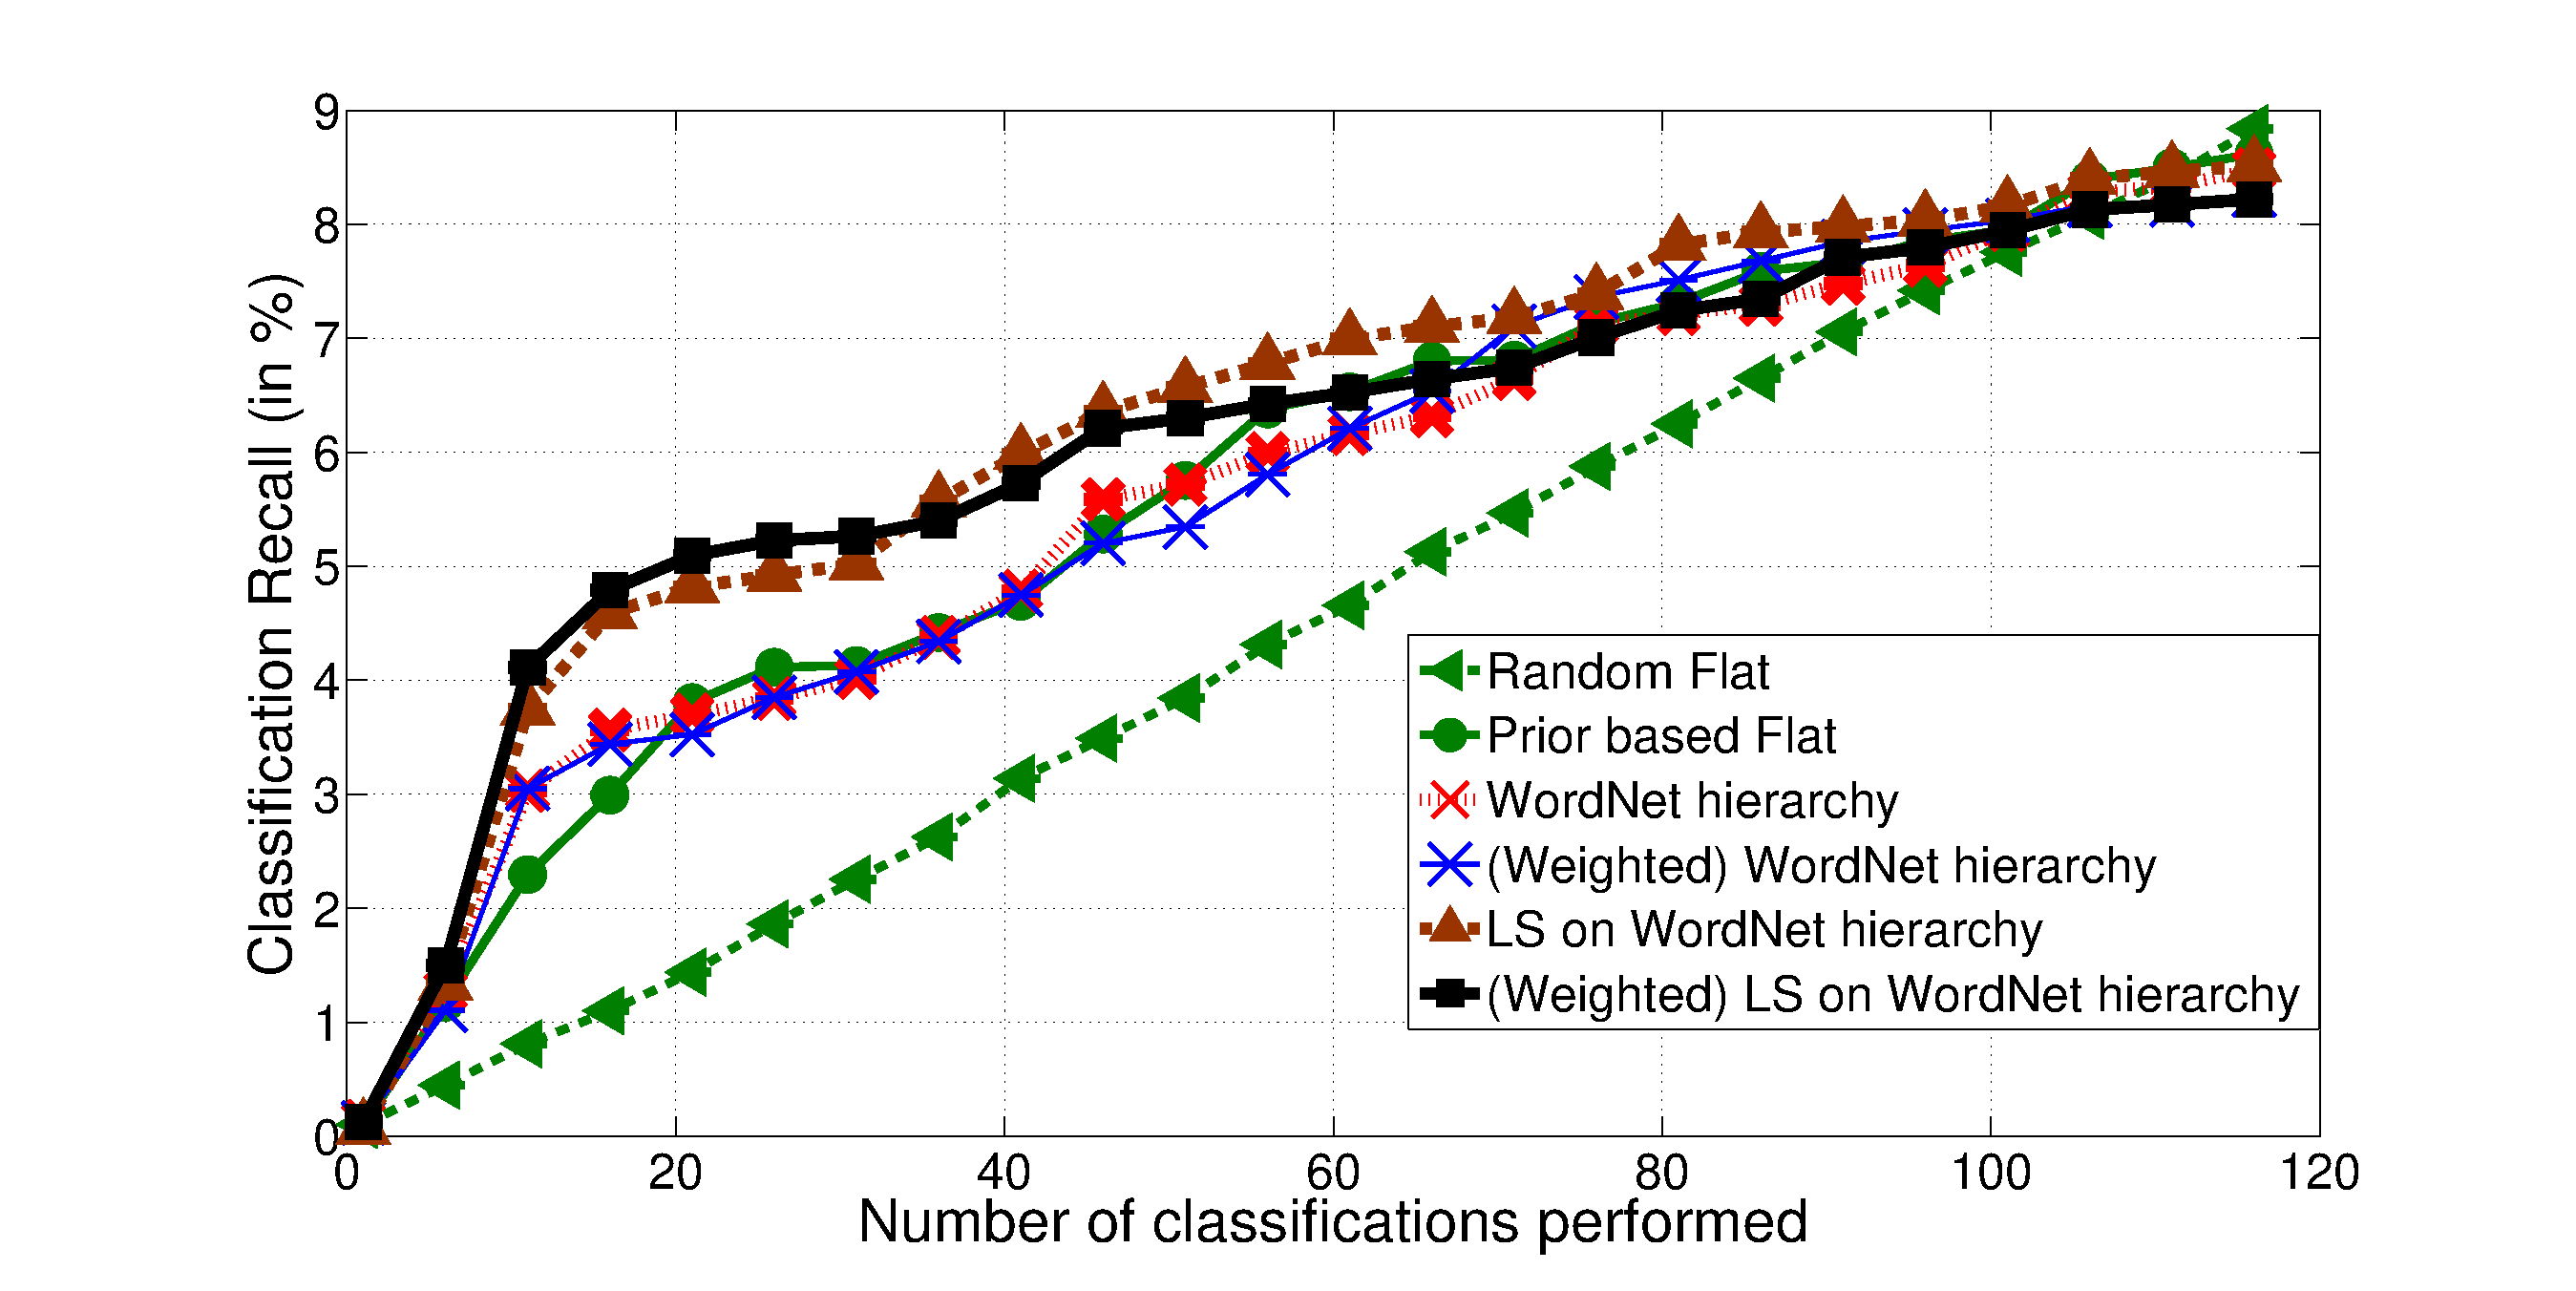
\includegraphics[width=\linewidth]{FastTagPredFWS117topK}
%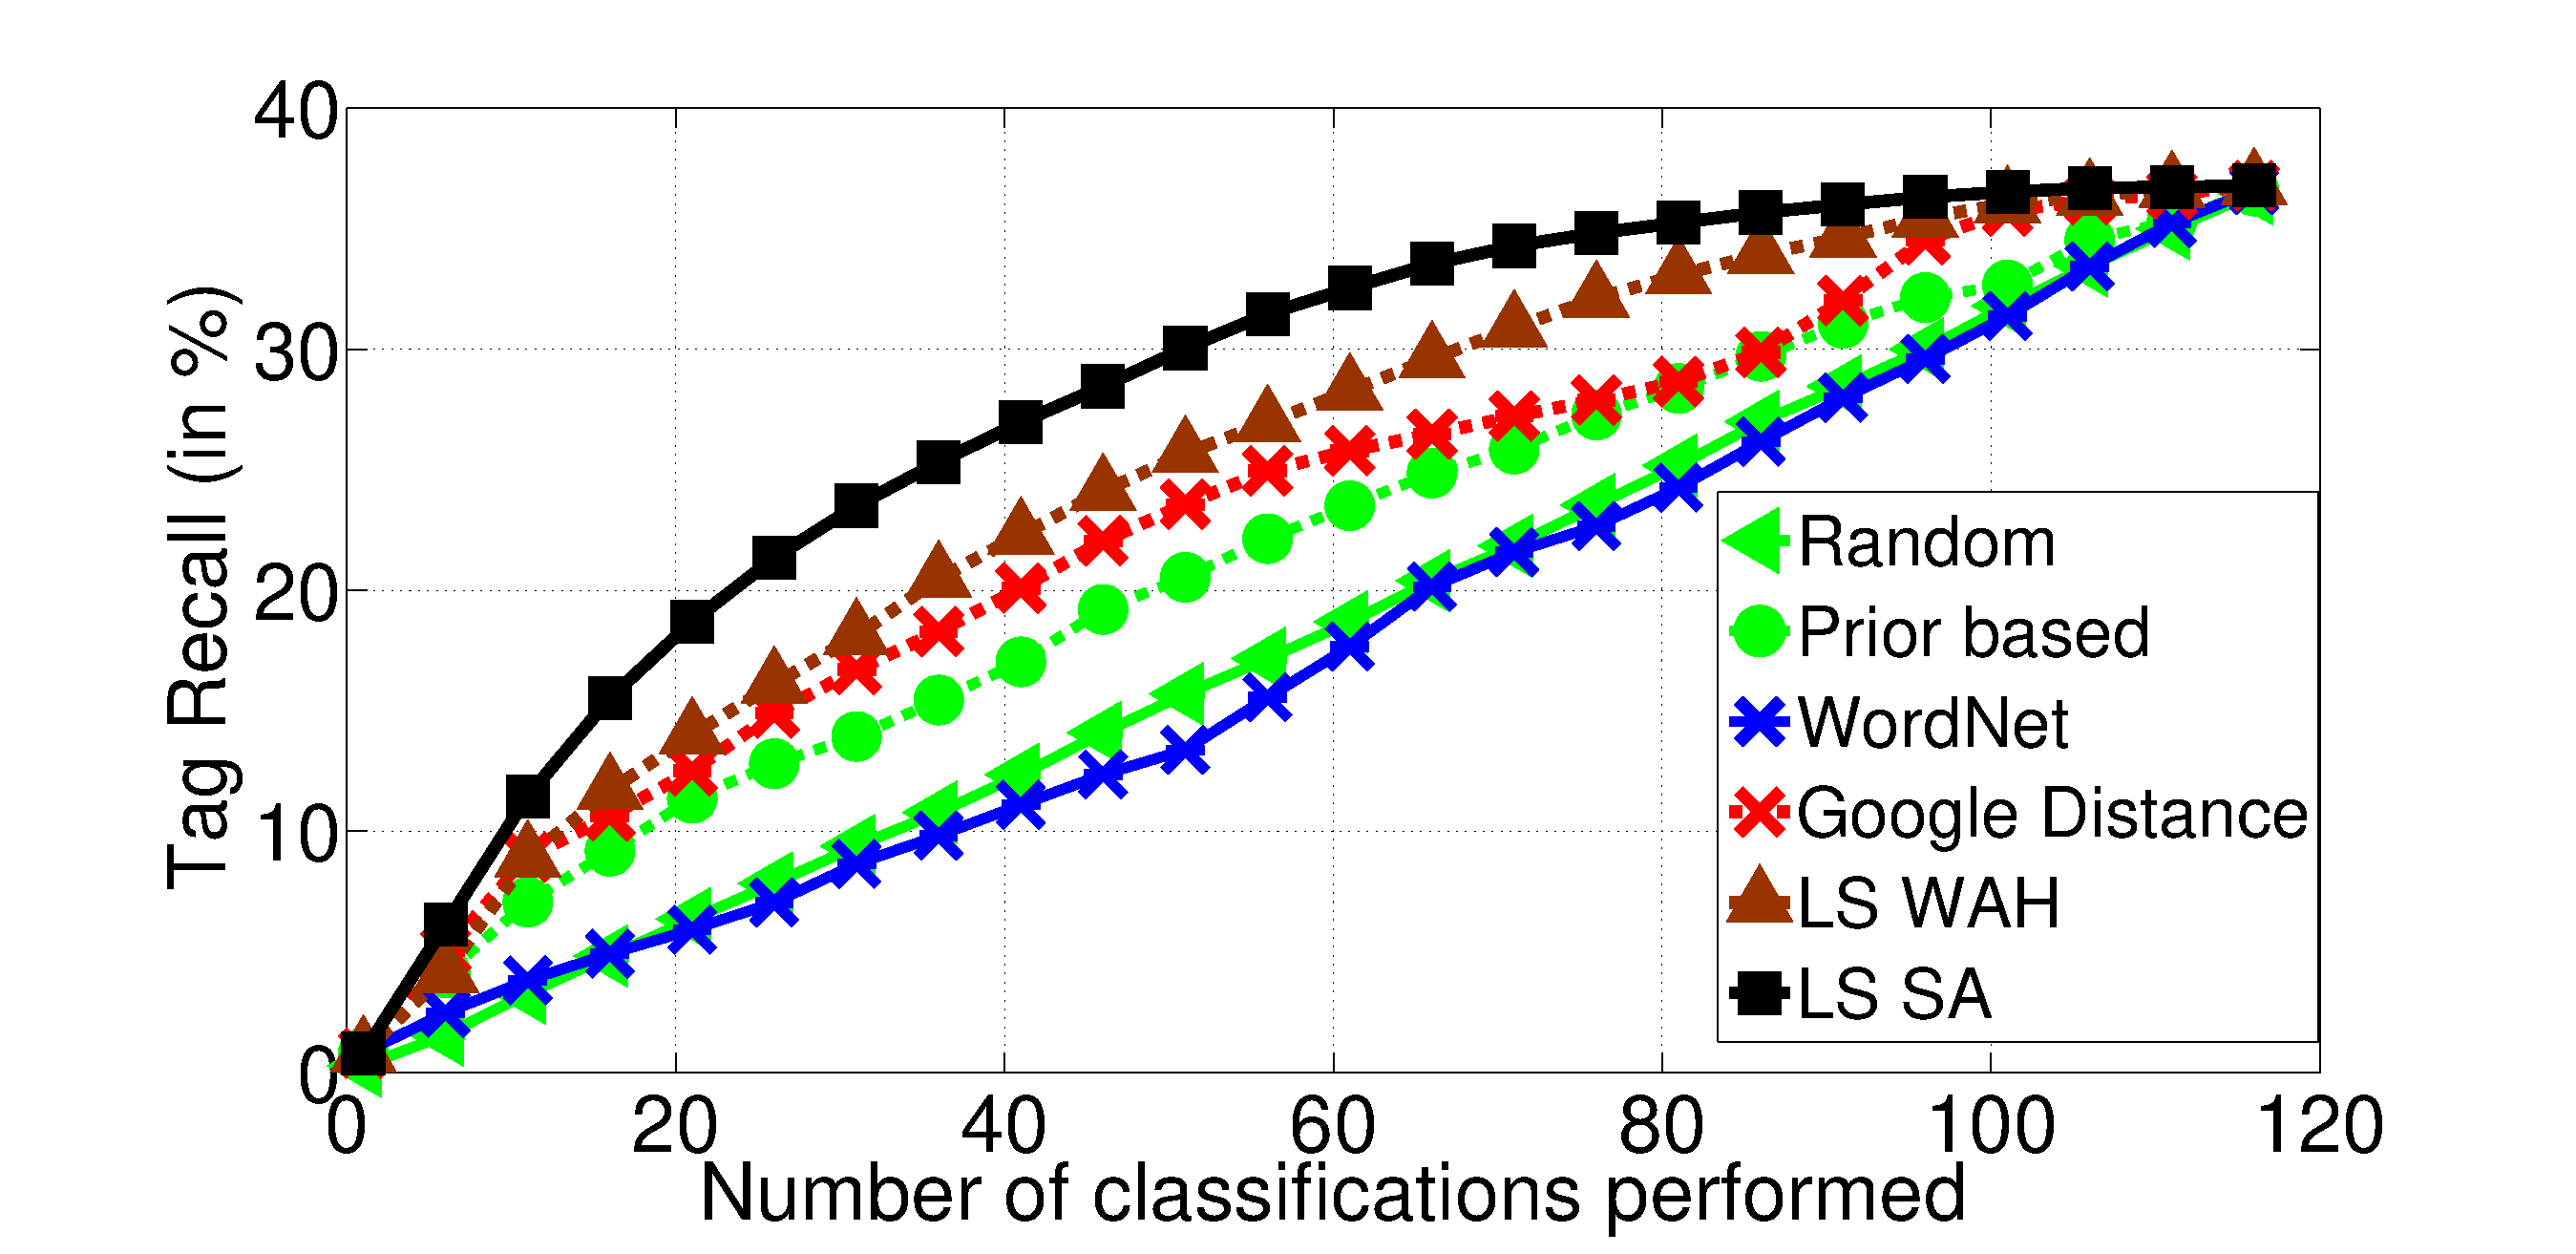
\includegraphics[width=\linewidth]{Journal_FastTagPredResults_LowerThreshMinpt5}
\centering
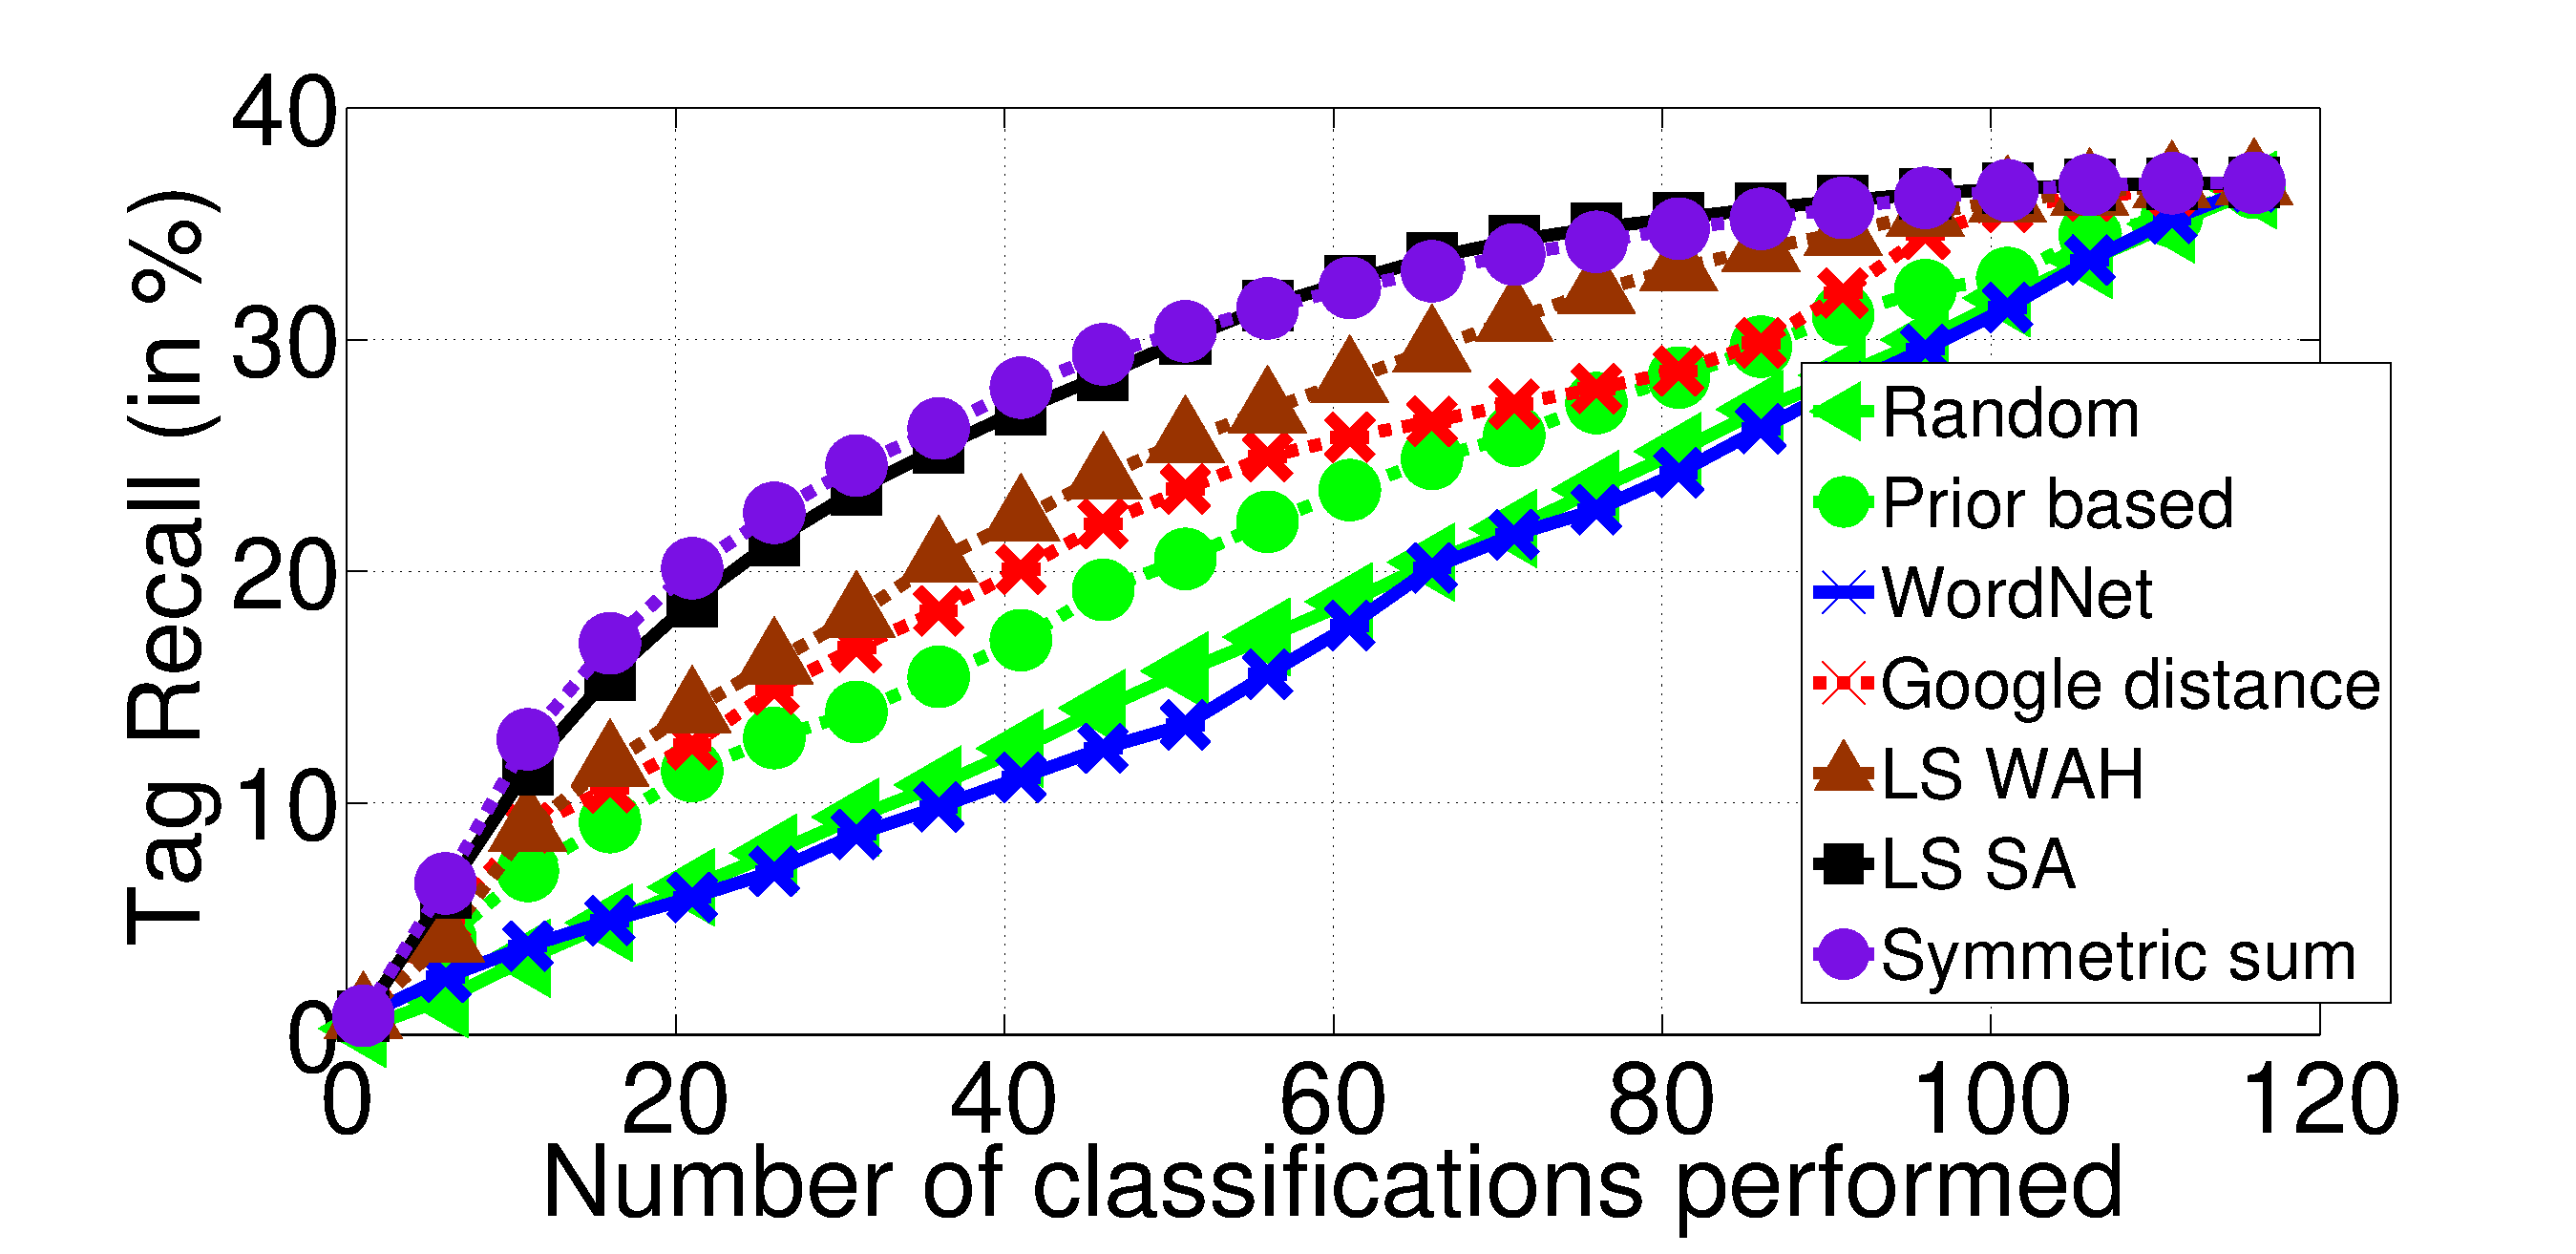
\includegraphics[width=0.65\linewidth]{TagTree/Rebuttal_FWS_Fast_LOWER}
\caption{\hl{Tag Recall obtained with respect to number of classifications performed for Flickr corpus. $\theta$ is chosen to be 0.33. } }
\label{fig:EfficientTagPredGraphFlickrLower}
\end{figure}
\begin{figure}[!htp]
%\epsfig{width=10cm,figure=FastTagPredGWS118topK.eps}
%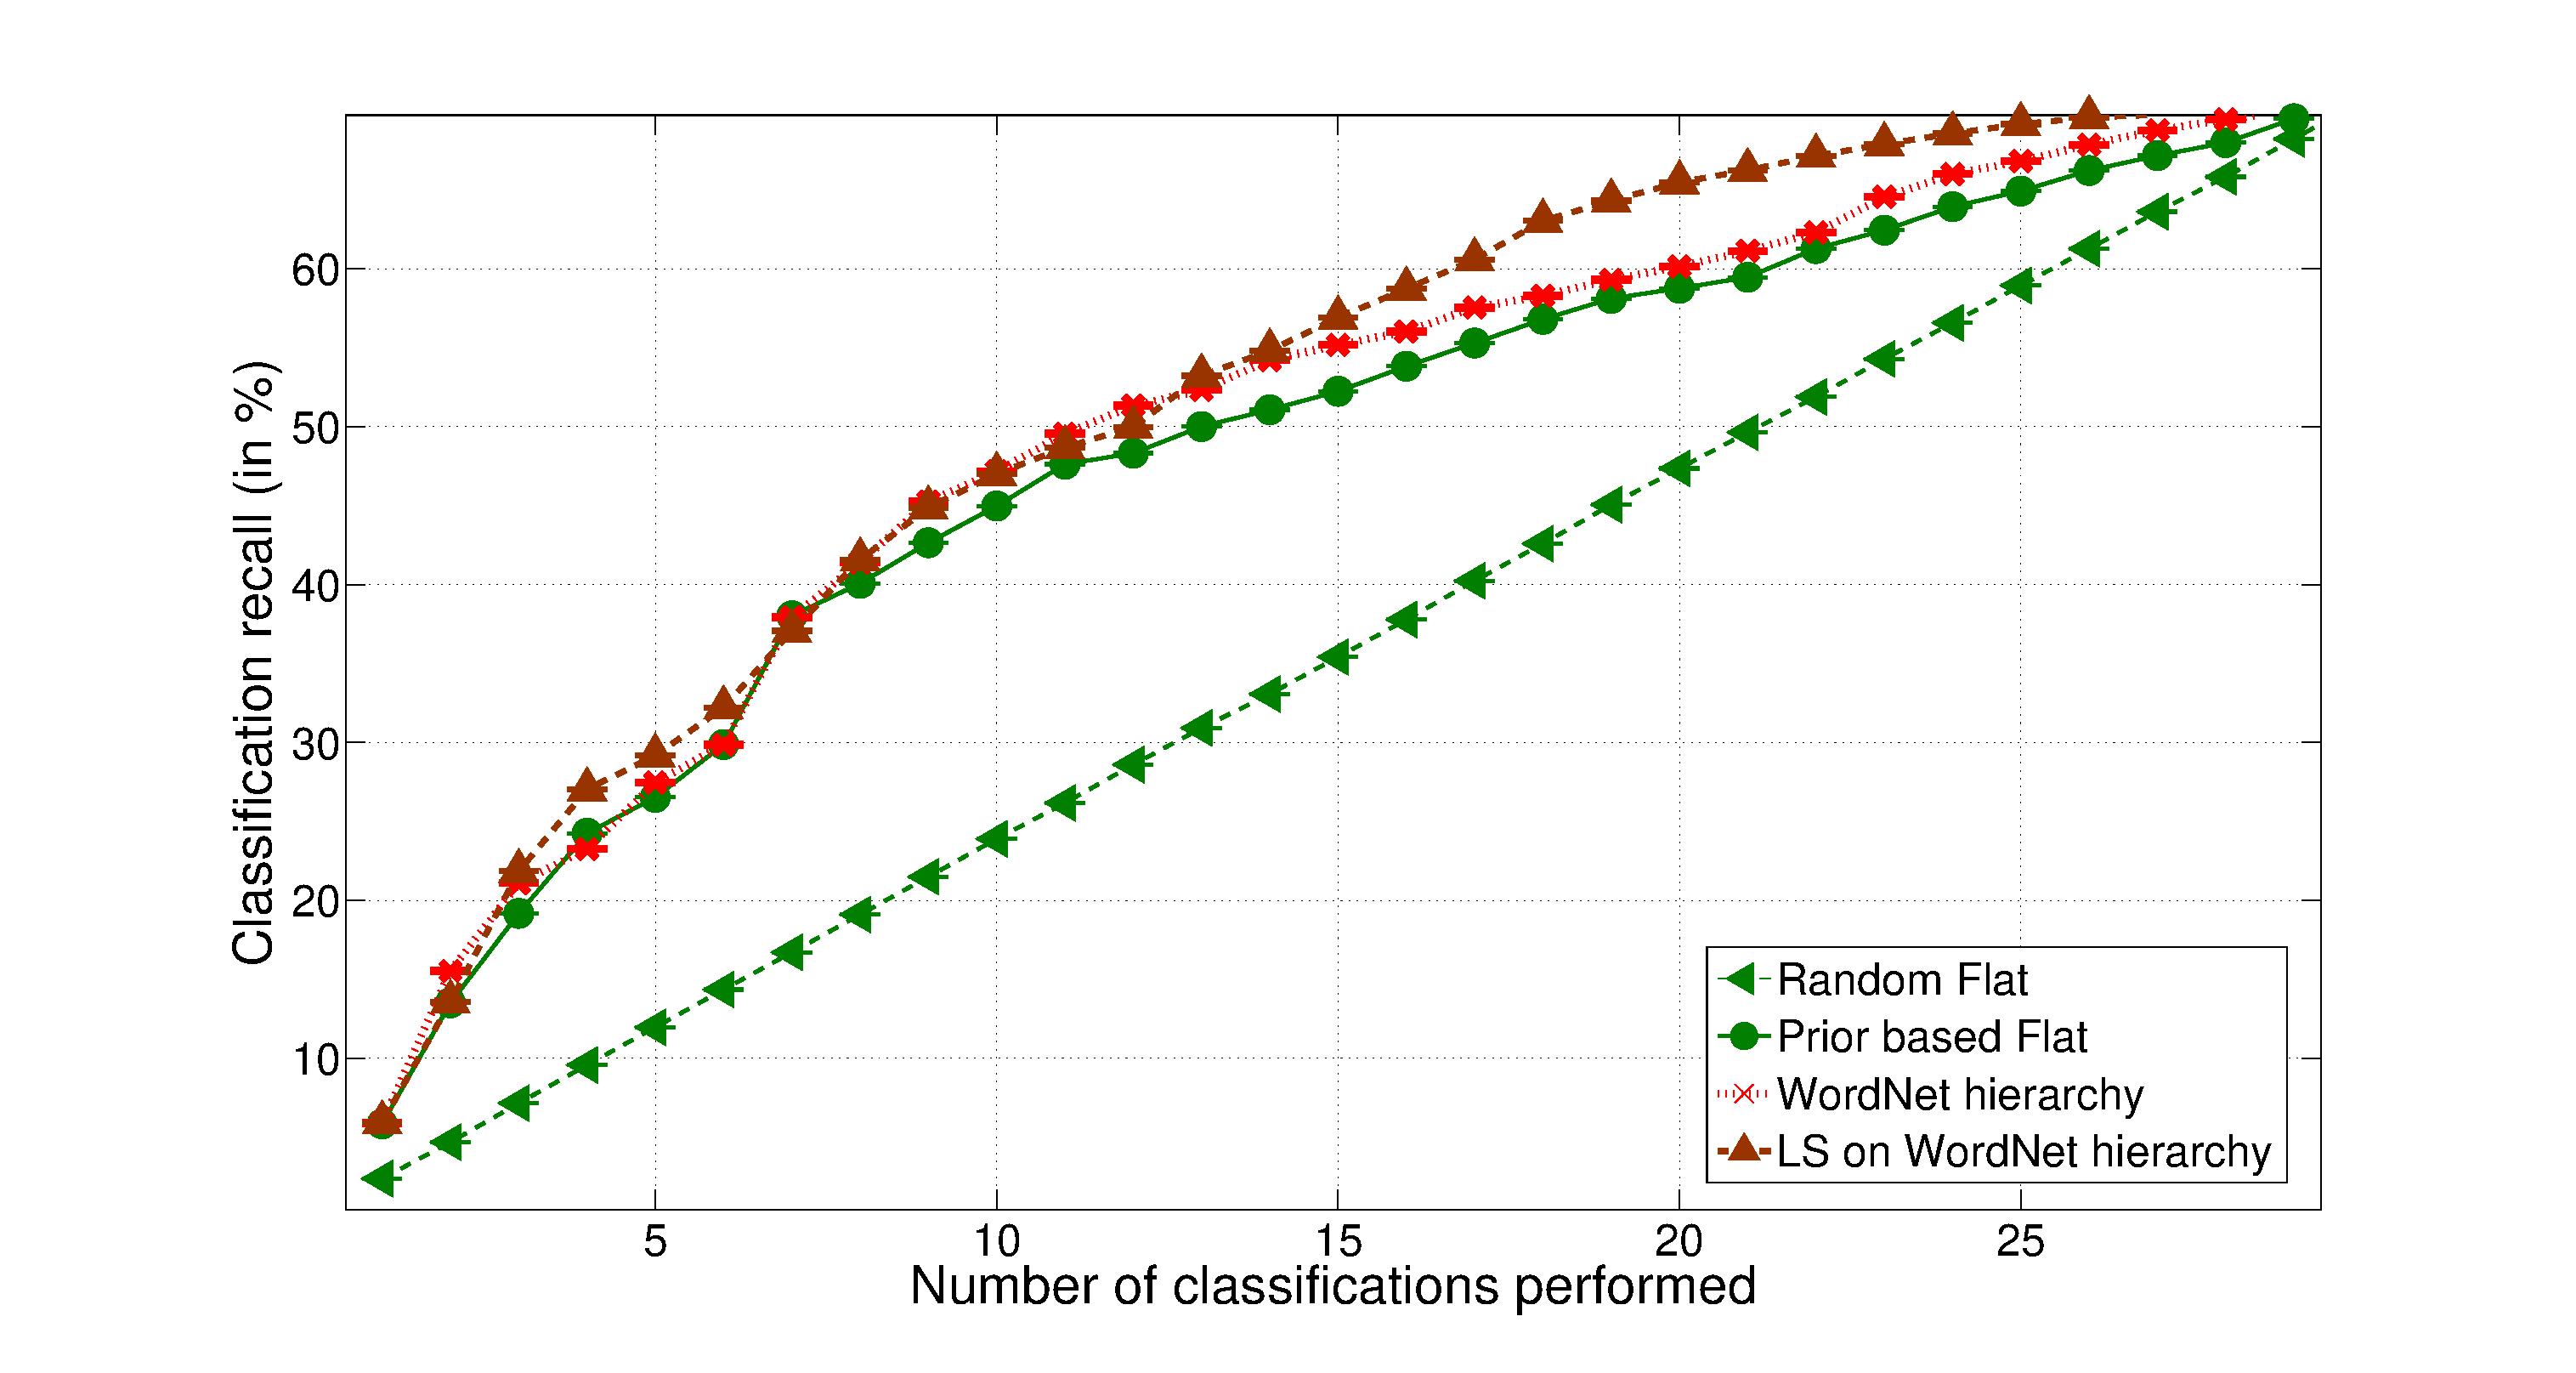
\includegraphics[width=\linewidth]{FastTagPredGWS118topK}
%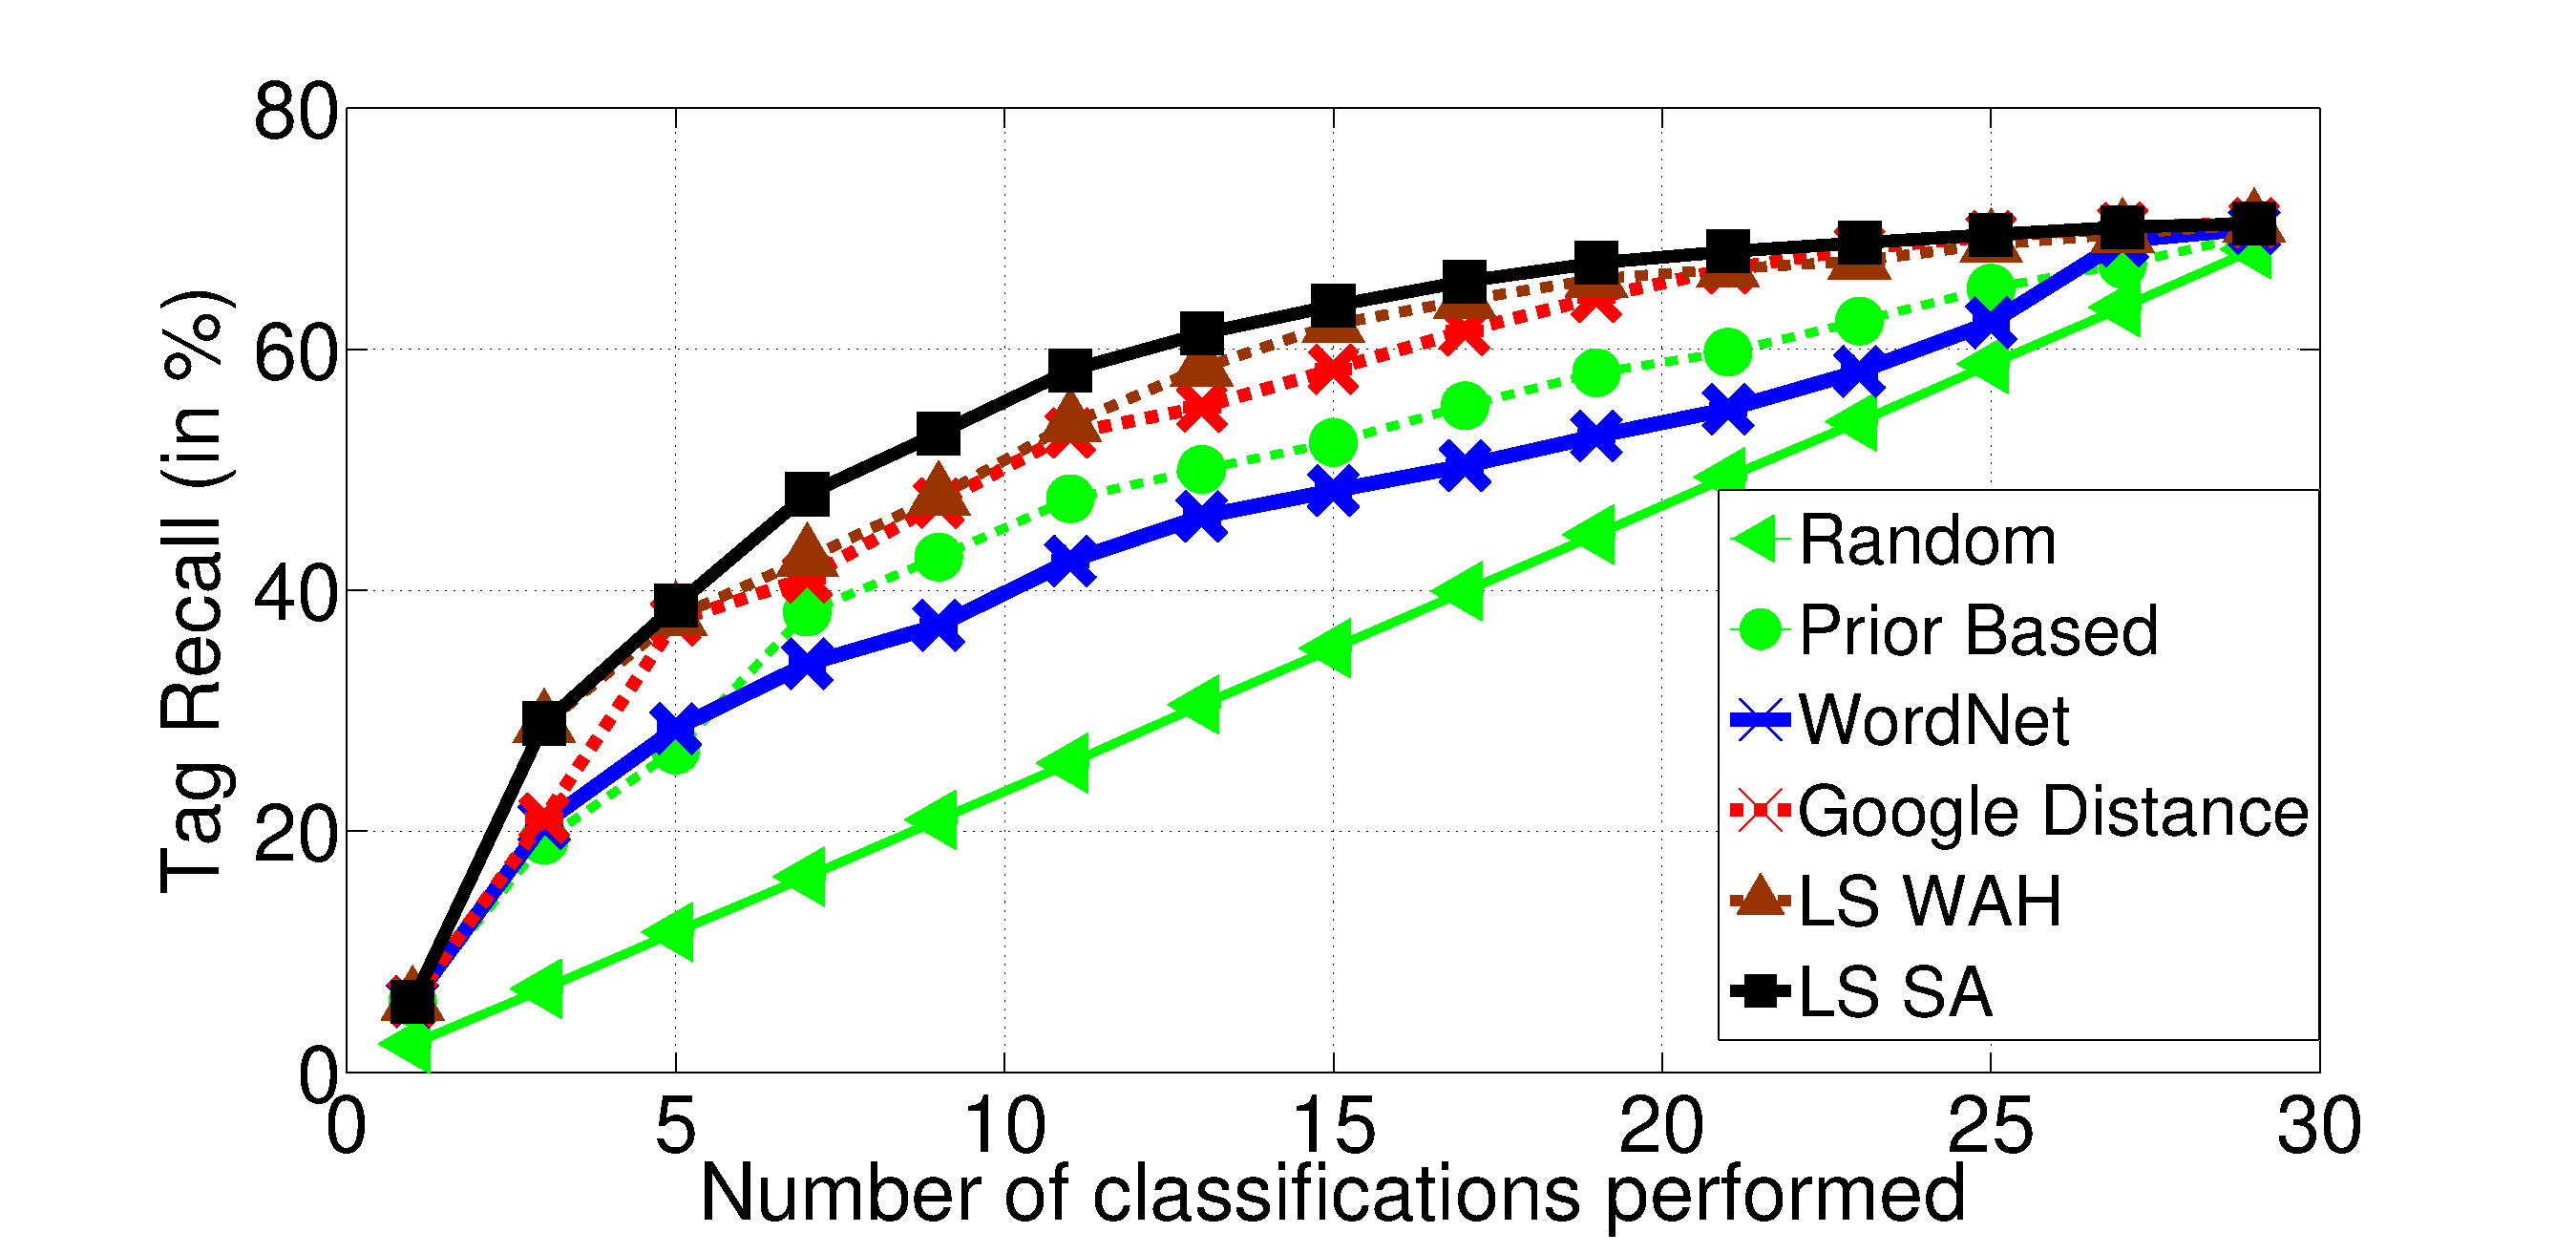
\includegraphics[width=\linewidth]{GWS30_FastTP_journal2}
\centering
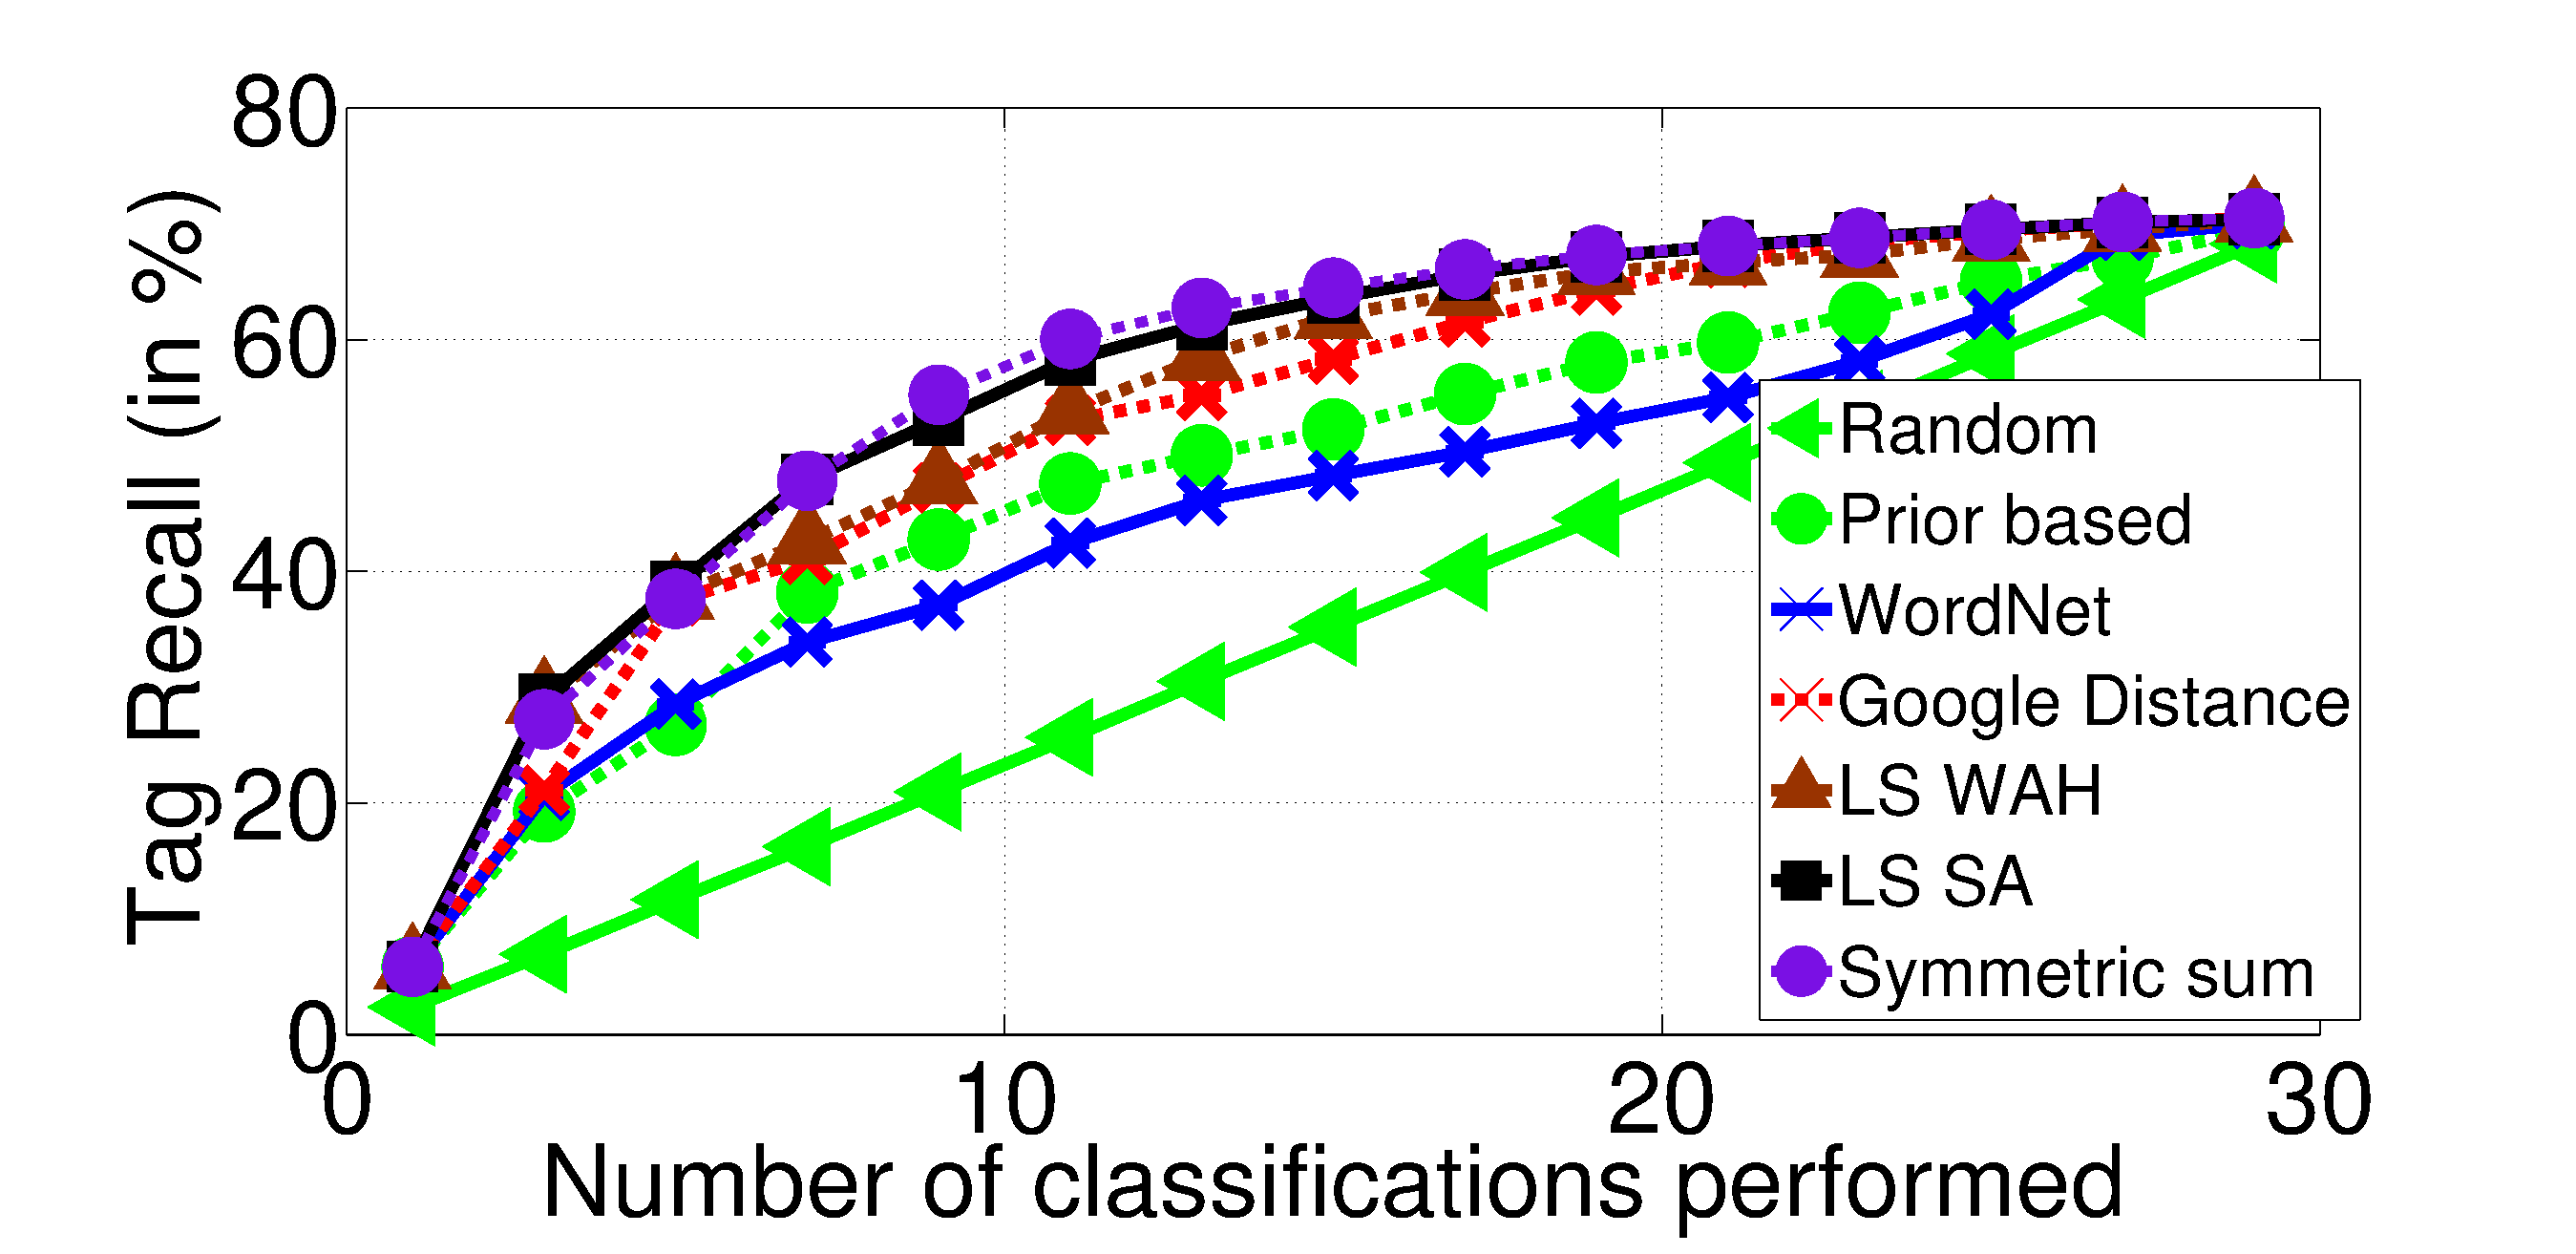
\includegraphics[width=0.65\linewidth]{TagTree/Rebuttal_FastTP_GWS}
\caption{\hl{Tag Recall obtained with respect to number of classifications performed for Stock images corpus. $\theta$ is chosen to  be 0.5. }}  
\label{fig:EfficientTagPredGraphGetty}
\end{figure}

\section{Robustness Analysis} \label{sec:Robustness}
We provide an analysis of the robustness of the proposed approach for constructing ontological tag trees. \hl{For the purpose of this section, we refer to the resource tag data using which the tag tree is constructed, as training data. The resource tag data over which the constructed tag tree is tested for evaluation purpose, is referred to as the test data}. \hl{As seen in Section {\ref{sec:Expts}}, the LS-SA method has consistently outperformed LS-WAH across different corpora and for both data-driven tasks}. Therefore, in this section we only study the robustness of the LS-SA method, i.e., the proposed local search based approach using Similarity Approximation based objective function (\ref{eq:ObjFnSimApprox}). In order to evaluate the constructed tag trees under various scenarios, we provide evaluation using tag prediction task as detailed in Section~\ref{subsec:TagPred}. \hl{Annotated image corpora are used for this purpose.} We study the robustness of proposed approach with respect to label noise, difference between training and test data, and the size of training data. These are discussed in detail below. 
\subsection{Robustness to Label Noise in Training Data}
\label{sec:RobustNoise}
\hl{As described in Section~{\ref{sec:Introduction}}, a vast majority of the user generated data available over the Internet has noisy labels (tags) associated with the resources}. We study the effect of different degrees of label noise on the tag tree constructed from such a noisy corpus. Fundamentally, we attempt to understand how robust the proposed tag tree construction approach is, to different degrees of label noise. We also attempt to answer questions such as - how much noise is too much for tag tree construction? 
\begin{figure}
%\epsfig{width=10cm,figure=VaryFWSorNoisewithGWSTPAccVary.eps}
%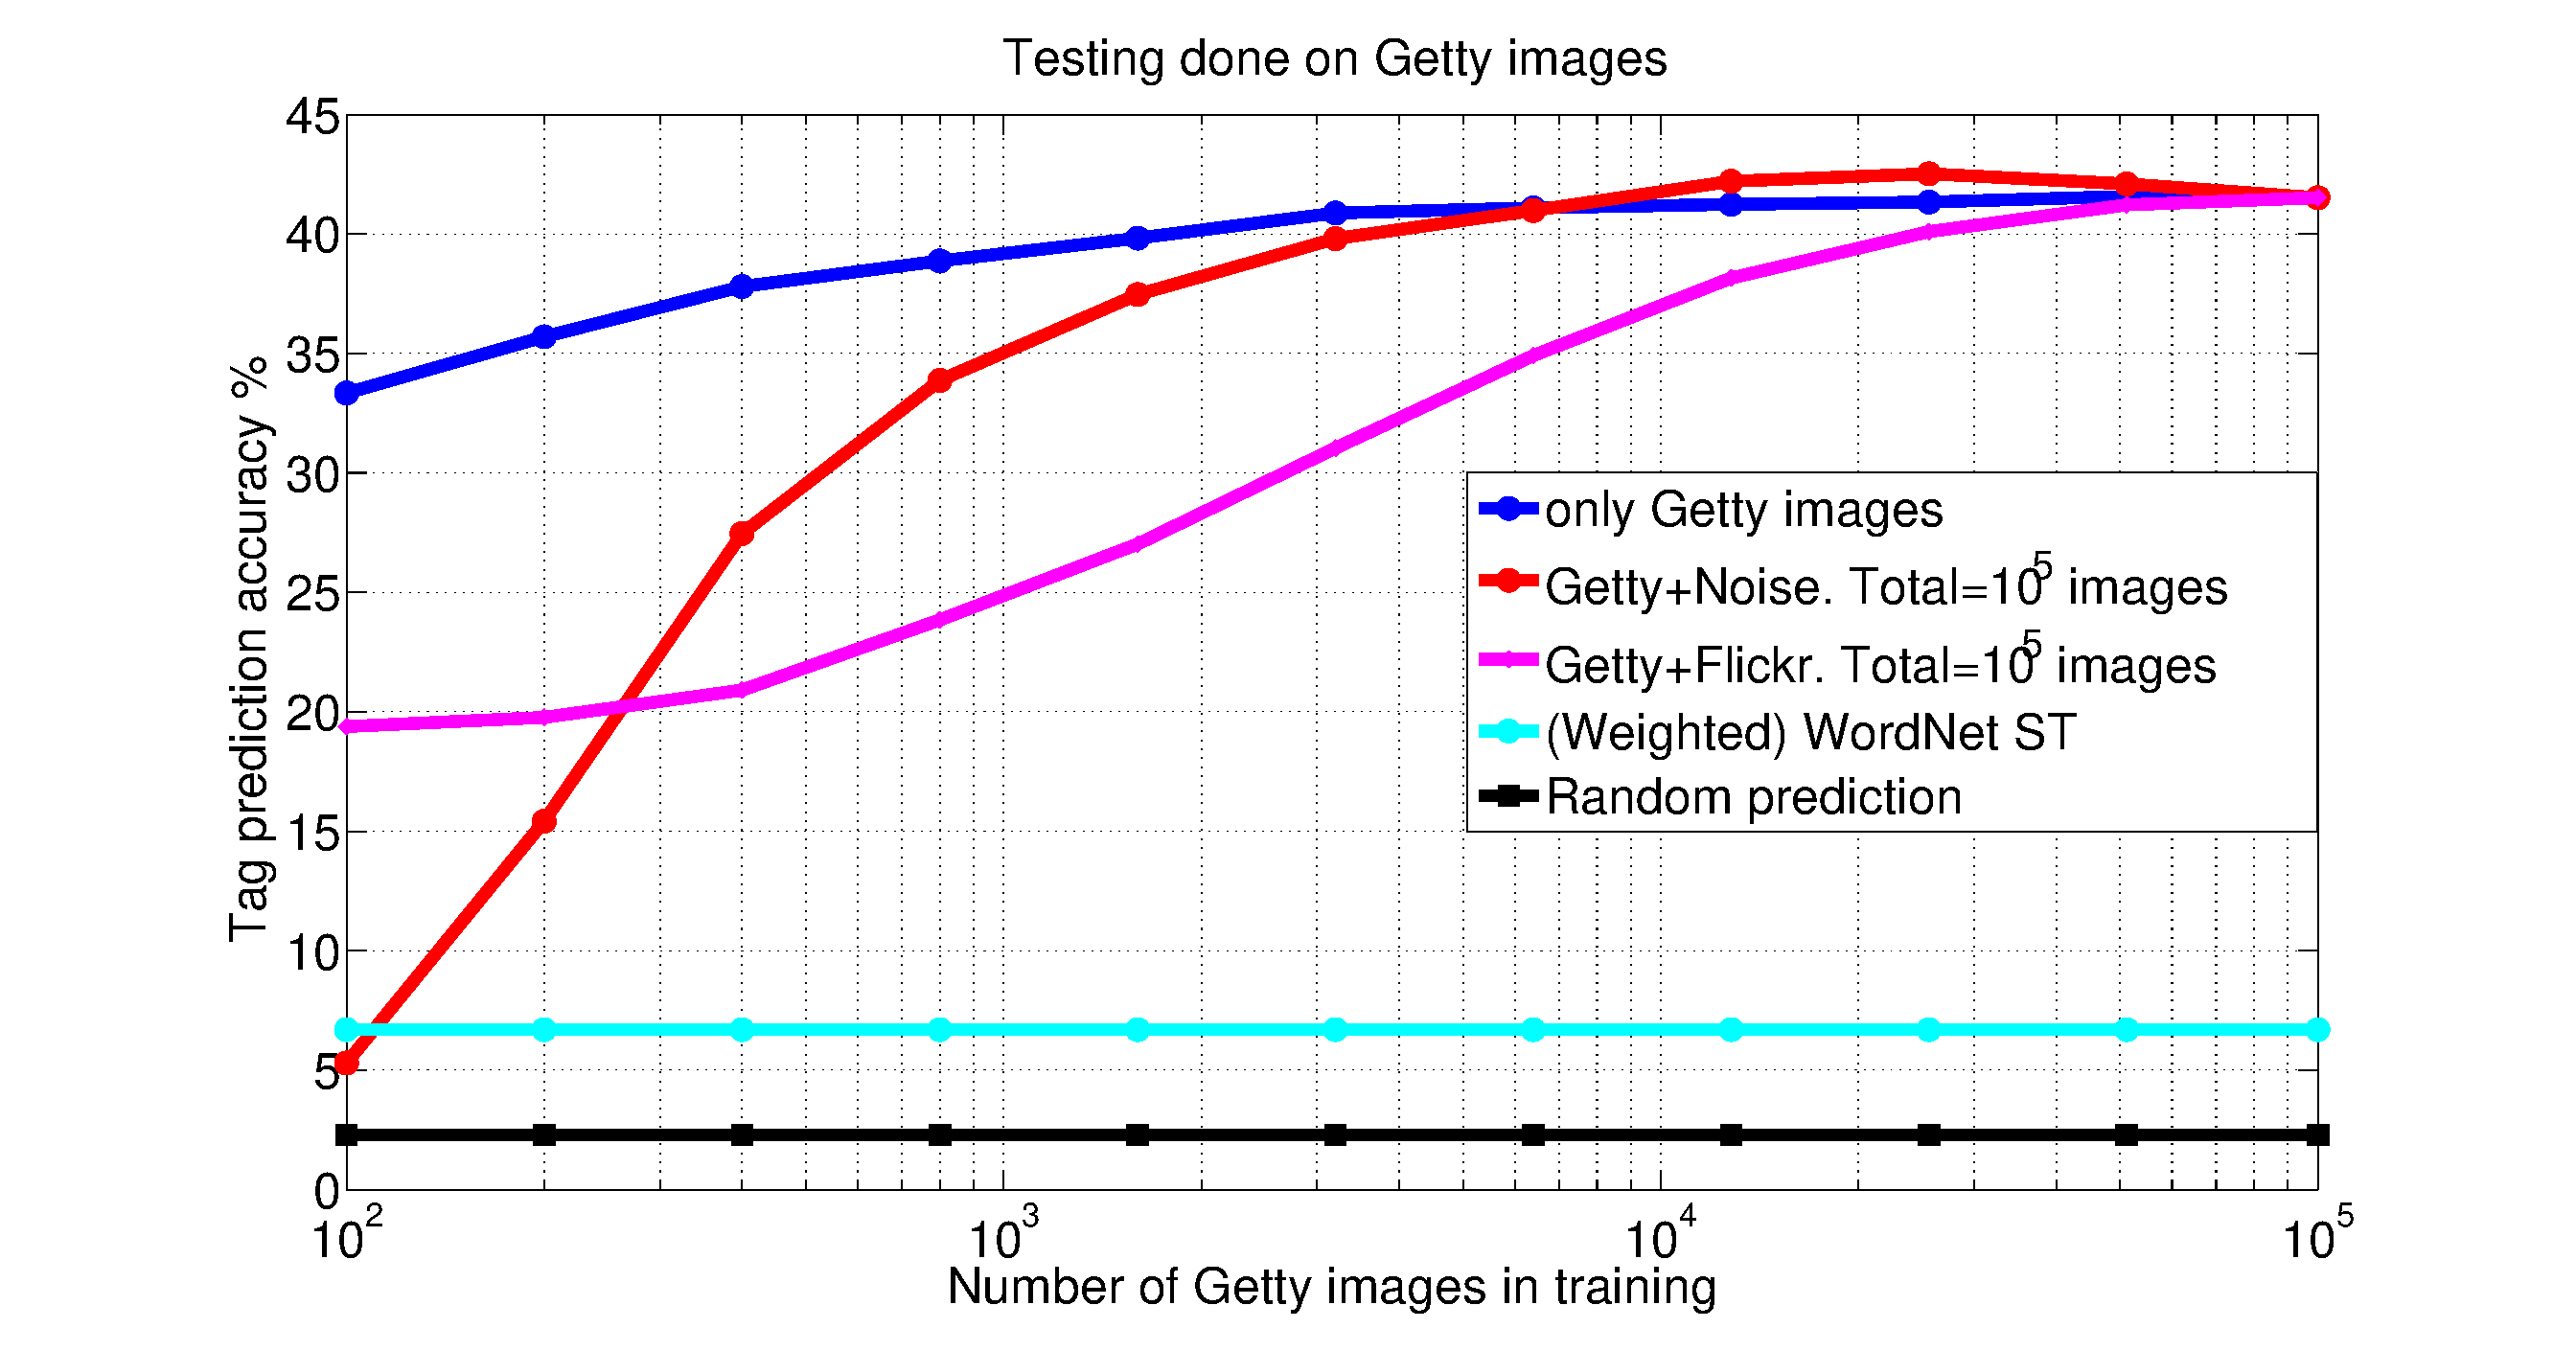
\includegraphics[width=\linewidth]{VaryFWSorNoisewithGWSTPAccVary}
\centering
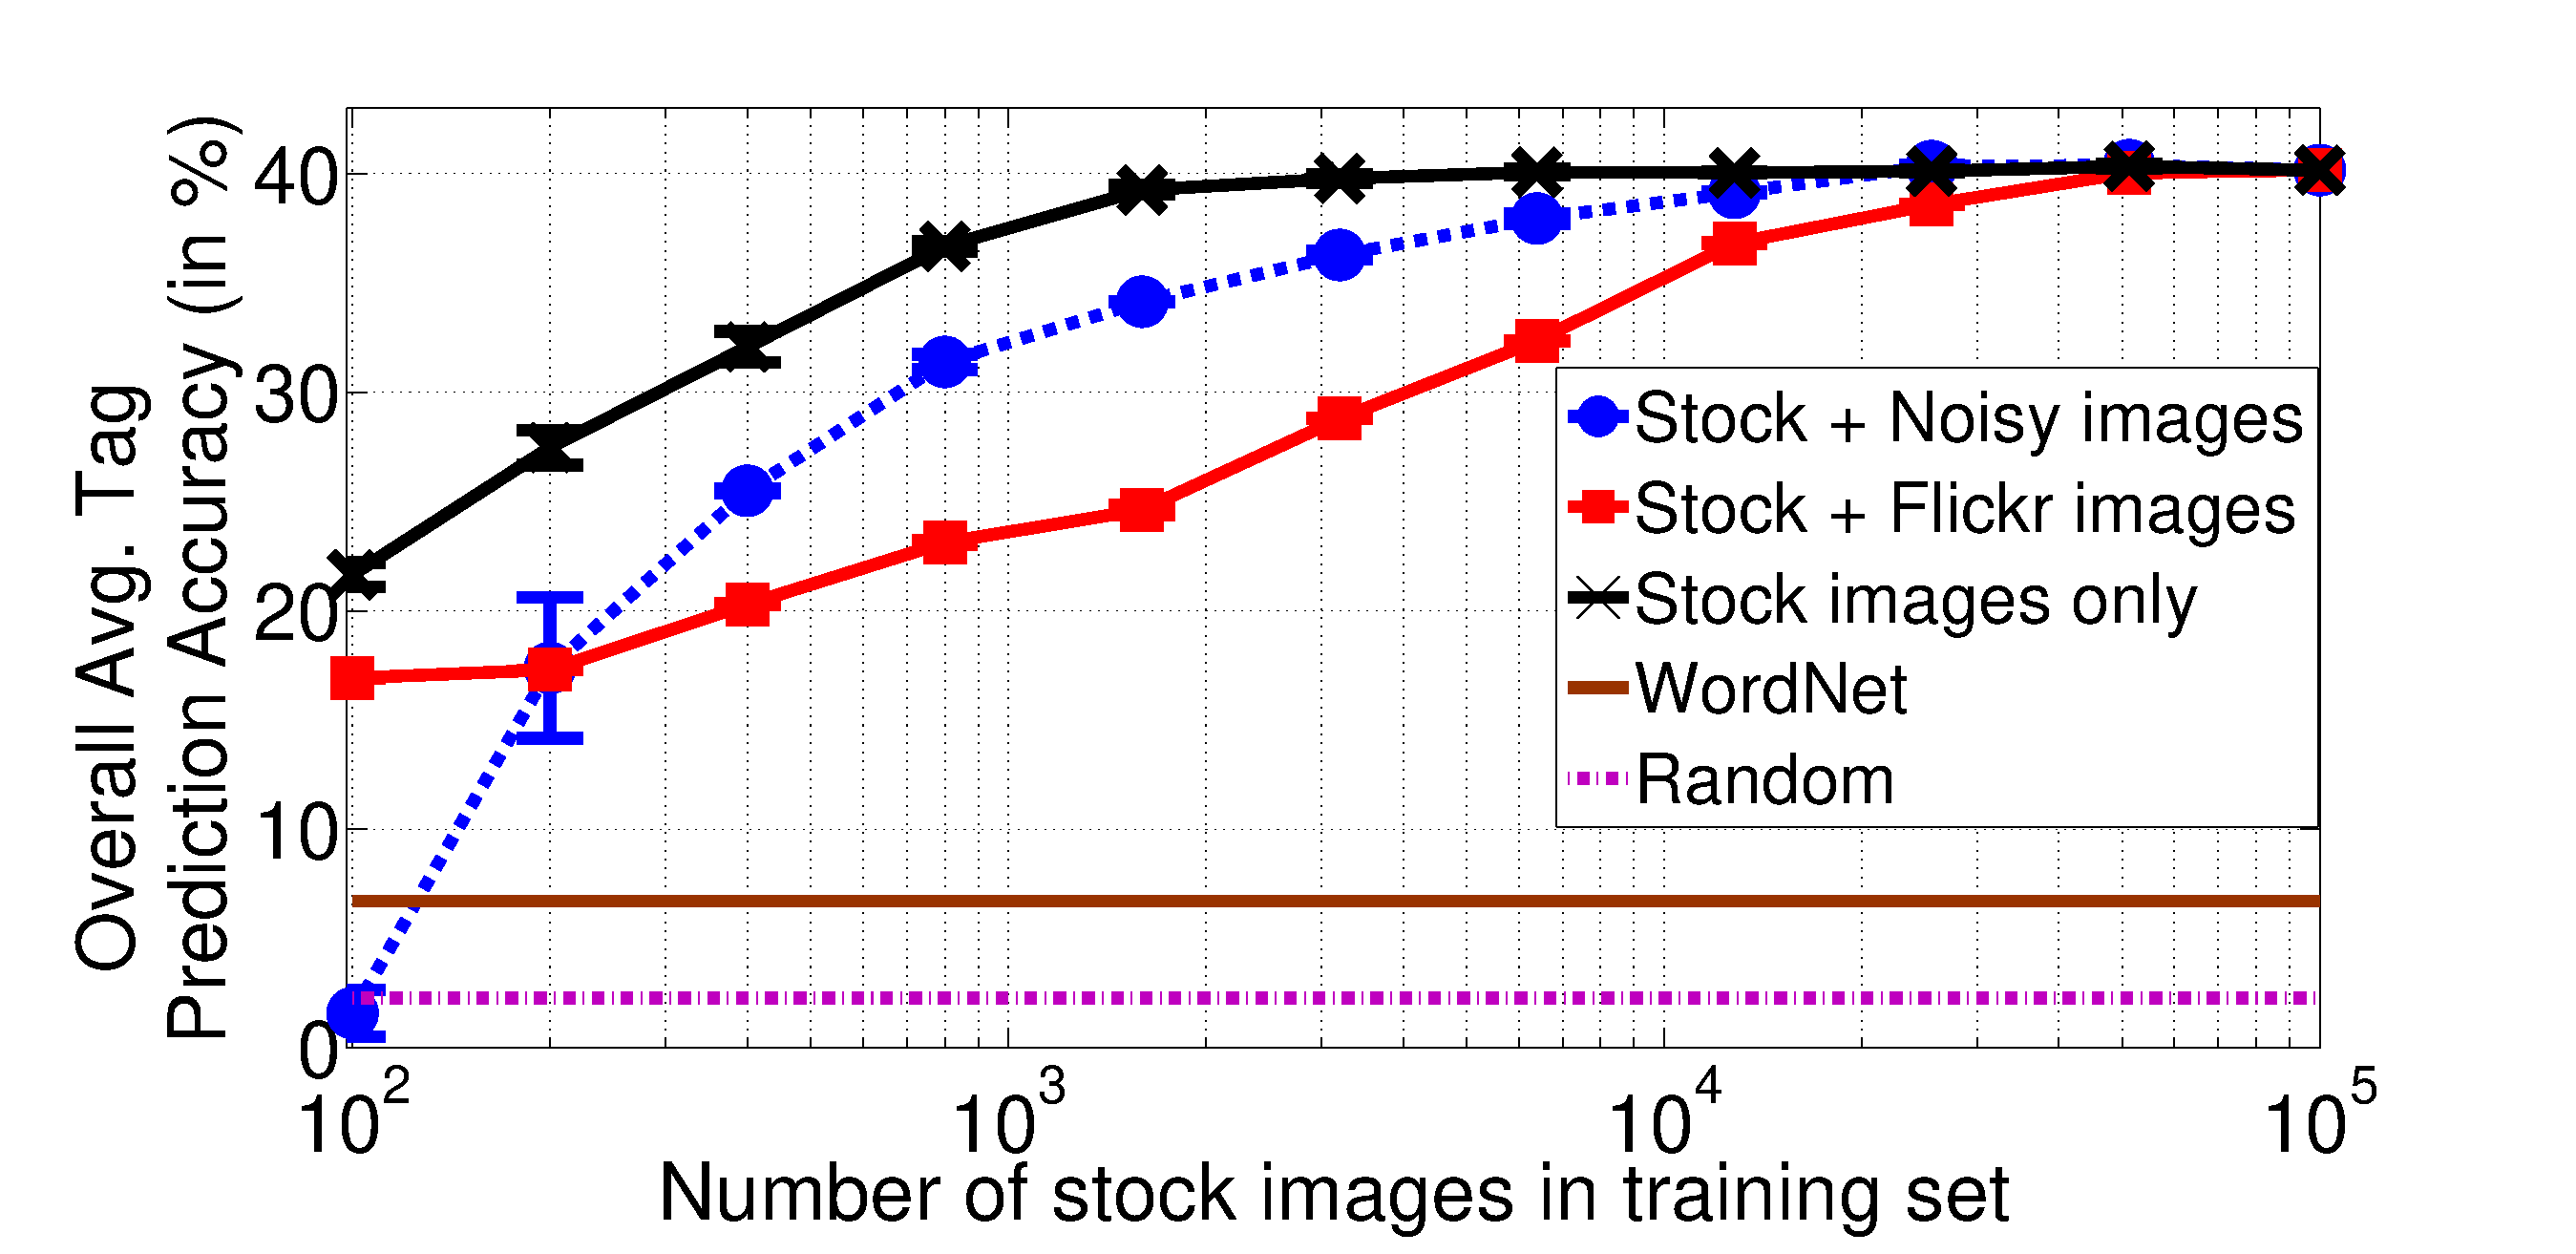
\includegraphics[width=0.65\linewidth]{TagTree/journal_RobustnessFig}
\caption[Robustness analysis using Overall Tag Prediction Score (in \%) obtained by proposed approach in Section~\ref{sec:TagPredUsingGraph}. ]{Overall Tag Prediction Score (in \%) obtained by proposed approach in Section~\ref{sec:TagPredUsingGraph}. The training set used to construct an ontological tag tree is formed by using certain number of stock images, with A) Flickr images, or B) noisy images, or C) none. Testing of the constructed tag tree is done on images of stock photos only. For comparison, the Overall Tag Prediction Accuracies for Random method, and WordNet method (as outlined in Section~\ref{sec:comparison}) are also provided. } 
%\vspace{-5mm}
\label{fig:AddNoiseTrainingData}
\end{figure}

We work with stock image corpus since stock images are professionally curated and have little to no label noise, thus providing a better control on the amount of noise in the experimental data. We select top 150 tags (keywords) from this corpus and remove those that do not occur in Flickr or in WordNet. This gives a set $\mathcal{T}$  of 108 tags. Each stock image has on an average 3 tags amongst $\mathcal{T}$. A total of 100,000 stock images are used in training set and 50,000 stock images in the test set. In order to simulate varying degrees of label noise in training set, we replace stock images in the training data with artificially created images with noisy tags. The total number of training images (stock images and noisy images) is kept constant at 100,000. The artificially created noisy images are defined as images having exactly 3 randomly chosen tags from $\mathcal{T}$. The test set is not varied.  Fig. ~\ref{fig:AddNoiseTrainingData} shows the variation of Overall Tag Prediction Accuracy (\%) as defined in Section \ref{subsec:TagPred}, with number of images that were from stock images in the training set. It can be seen that even with 87.2\% noisy images in the training set, the performance of the constructed tag tree (39\%) is very close to the performance when there are no noisy images at all (40\%). Even when 99.2\% of the images in training set are noisy, the Overall Tag Prediction Accuracy is 31.4\%. An explanation for such performance even at high levels of noise is that the noisy images have uniformly random distribution of tags. The overall effect of adding noisy images to a corpus can be understood as adding certain intensity of white noise to the co-occurrence counts between tags. Unless the noise intensity dominates the corpus statistics, the relative order of pair-wise connections between tags remains fairly unchanged. In other words, since the noisy images have no strong biases towards specific tag-pairs, the performance of tag trees constructed using such a hybrid training set is not severely affected. 

\subsection{Robustness to Difference between Training and Test Data}
\label{sec:RobustDifference}
In several machine learning applications, the data over which a model is trained has certain amount of distributional difference as compared to the data over which it is tested. Looking at the construction of tag tree as model training, the degree to which a tag tree will be effective on a test set is a function of the difference between the test set and the training set using which the tag tree is constructed. Here we study how the performance of a tag tree varies for different degrees of difference between the training and the test sets. We utilize the same stock images corpus as used in Section~\ref{sec:RobustNoise}. In order to vary the difference between training and test sets, we replace varying number of stock images in training set with images from Flickr corpus (Section~\ref{sec:Datasets}). The total number of images (stock images and Flickr images) used for training of tag tree is kept constant at 100,000. Fig.~\ref{fig:AddNoiseTrainingData} shows the variation of Overall Tag Prediction Accuracy (\%) with number of images that were from stock images in the training set. It is interesting to note that for the same number of stock images, adding completely noisy images leads to better performance than adding Flickr images. For instance, for the case when 99.2\% of training images are from Flickr, performance of the constructed tag tree (23.1\%) is seen to be substantially worse than when 99.2\% of training images are noisy (31.4\%). The reason for this is that the tag distribution in Flickr corpus is not random, unlike in the case of noisy images. As a result, there are strong relationships between tags in Flickr corpus that are absent in stock image corpus. Constructing a tag tree on such a hybrid corpus attempts to capture corpus statistics of varying numbers of Flickr images and stock images, and in the process, is less effective at capturing the relationships that were present in the test data that has only stock images. 

\subsection{Size of Training Data}
\label{sec:RobustSize}
In this section, we study the effect of size of training set on construction of tag trees. Fig. ~\ref{fig:AddNoiseTrainingData} shows the variation of Overall Tag Prediction Accuracy (\%) with number of stock images in the training data. Here the size of training set is equal to the number of stock images in it and there are no Flickr images or noisy images. The performance of constructed tag tree improves with size of training data and almost saturates after certain number of training images. This is quite similar to the variation in performance of most machine learning models with the size of data over which they are trained. The performance of constructed tag tree from only 800 stock images is very close to the performance when 100,000 images are used. Even when only 100 stock images are used, the constructed tag tree performs much better than the tag trees using 100 stock images with 99900 Flickr or noisy images. Based on above, one can conclude that for the construction of ontological tag trees, it is better to use fewer training images than a larger set which is noisy or dissimilar to the test set.  
\comment{
\begin{figure}[htbp]
\centering
\begin{tabular}{p{2.2cm} p{2.2cm} p{3cm}}
\centering
\epsfig{width=2cm,height=2.8cm,figure=TagTree/figures/3569597369_690c84559a.eps} & %32965350@N00
\epsfig{width=2cm,height=2.8cm,figure=TagTree/figures/183307784_ca9034cc51.eps} & %85598619@N00
\epsfig{width=2.8cm,height=2cm,figure=TagTree/figures/180824073_fc5f017f46.eps}\\ %22768390@N00
(a){\bf holiday, island}, travel, vacation, water&
(b){\bf england, street}, building, london,uk&
(c){\bf germany, travel}, deutschland, europe, summer\\
\end{tabular}
\caption{A few examples where the local search based refinement was able to predict two of the three tags correctly, given two original tags (shown in bold). Tag prediction based on WordNet did not result in correct prediction for these examples. The Flickr owner and photo ids of these images are (32965350@N00,3569597369), (85598619@N00,183307784), (22768390@N00,180824073) respectively.}
\label{fig:examples}
\end{figure}
}
\begin{figure*}
        \centering
	\captionsetup{justification=raggedright,
	singlelinecheck=false
	}
        \begin{subfigure}[b]{0.16\textwidth}
                \includegraphics[width=0.8\textwidth]{TagTree/Flickrimg/777b9480-f735-3d7a-aa91-dba84cea8bf2.jpeg} 
                \caption{\textbf{Seen}: highway, road \\ \textbf{Unseen}: route, shield, sign }
                \label{fig:posex1}
        \end{subfigure}%
	\; \vline
        \; %add desired spacing between images, e. g. ~, \quad, \qquad etc.
          %(or a blank line to force the subfigure onto a new line)
        \begin{subfigure}[b]{0.17\textwidth}
                \includegraphics[width=0.8\textwidth]{TagTree/Flickrimg/e3bb5574-1a09-32cf-9f22-1a9eb81af7c2.jpeg}
                \caption{\textbf{Seen}: austin, \\ band \\ \textbf{Unseen}: music, texas, tx }
                \label{fig:posex2}
        \end{subfigure}%
	\; \vline
        \; %add desired spacing between images, e. g. ~, \quad, \qquad etc.
          %(or a blank line to force the subfigure onto a new line)
        \begin{subfigure}[b]{0.17\textwidth}
                \includegraphics[width=0.8\textwidth]{TagTree/Flickrimg/7c52f0a2-78ae-3b9b-9dd0-f131124750f5.jpeg}
                \caption{\textbf{Seen}: england, europe \\ \textbf{Unseen}: london, travel, uk }
                \label{fig:posex3}
        \end{subfigure}%
	\; \vline
        \; %add desired spacing between images, e. g. ~, \quad, \qquad etc.
          %(or a blank line to force the subfigure onto a new line)
        \begin{subfigure}[b]{0.16\textwidth}
                \includegraphics[width=0.8\textwidth]{TagTree/Flickrimg/b03623e7-e6cf-3e96-97cc-a7117c776614.jpeg}
                \caption{\textbf{Seen}: art, dc \\ \textbf{Unseen}: graffiti, street, washington }
                \label{fig:posex4}
        \end{subfigure}%
	\; \vline
        \; %add desired spacing between images, e. g. ~, \quad, \qquad etc.
          %(or a blank line to force the subfigure onto a new line)
        \begin{subfigure}[b]{0.17\textwidth}
                \includegraphics[width=0.8\textwidth]{TagTree/Flickrimg/8efd5e1c-6d83-37af-91a2-1484a9d823b3.jpeg}
                \caption{\textbf{Seen}: concert, england\\ \textbf{Unseen}: london, music, uk }
                \label{fig:posex5}
        \end{subfigure}
        \caption[Example images where LS-SA method gave 100\% tag prediction accuracy when the first two tags were seen and the next three were unseen and predicted. ]{Example images where LS-SA method gave 100\% tag prediction accuracy when the first two tags were seen and the next three were unseen and predicted. The Flickr owner and photo ids of these images are (dougtone@7975042008) ,  (elchupacabra@7023118527) , (jeffwilcox@159730021) , (daquellamanera@4678084101) , (martinrp@3832812191)  respectively. } \label{fig:positiveExs}
\end{figure*}

\begin{figure*}
        \centering
	\captionsetup{justification=raggedright,
	singlelinecheck=false
	}
        \begin{subfigure}[b]{0.16\textwidth}
                \includegraphics[width=\textwidth]{TagTree/Flickrimg/7a6b7ae7-7afb-3f90-92df-e67c0bd22a8a.jpeg}
                \caption{\textbf{Seen}: film, france \\ \textbf{Unseen}: holiday, \\ sky, snow \\ \textbf{Predicted}: paris, europe, bw }
                \label{fig:negex1}
        \end{subfigure}%
	\; \vline
        \; %add desired spacing between images, e. g. ~, \quad, \qquad etc.
          %(or a blank line to force the subfigure onto a new line)
        \begin{subfigure}[b]{0.17\textwidth}
                \includegraphics[width=0.8\textwidth]{TagTree/Flickrimg/ec4436dd-57b3-36af-94f6-64cf05294886.jpeg}
                \caption{\textbf{Seen}: china, family \\ \textbf{Unseen}: live, summer, \\ usa  \\ \textbf{Predicted}: photography, christmas, photo }
                \label{fig:negex2}
        \end{subfigure}%
	\; \vline
        \; %add desired spacing between images, e. g. ~, \quad, \qquad etc.
          %(or a blank line to force the subfigure onto a new line)
        \begin{subfigure}[b]{0.16\textwidth}
                \includegraphics[width=0.8\textwidth]{TagTree/Flickrimg/bf51a02f-baa1-3861-a300-12b5f654c456.jpeg}
                \caption{\textbf{Seen}: canada, \\ ocean \\ \textbf{Unseen}: red, sky, sunset \\ \textbf{Predicted}: sea, beach, water }
                \label{fig:negex3}
        \end{subfigure}%
	\; \vline
        \; %add desired spacing between images, e. g. ~, \quad, \qquad etc.
          %(or a blank line to force the subfigure onto a new line)
        \begin{subfigure}[b]{0.17\textwidth}
                \includegraphics[width=0.8\textwidth]{TagTree/Flickrimg/b339e52a-b87e-347a-8ba8-12502fc11443.jpeg}
                \caption{\textbf{Seen}: autumn, \\ black\\ \textbf{Unseen}: light, macro, night \\ \textbf{Predicted}: white, nature, bw }
                \label{fig:negex4}
        \end{subfigure}%
	\; \vline
        \; %add desired spacing between images, e. g. ~, \quad, \qquad etc.
          %(or a blank line to force the subfigure onto a new line)
        \begin{subfigure}[b]{0.18\textwidth}
                \includegraphics[width=0.45\textwidth]{TagTree/Flickrimg/acf2533e-69ac-3e2e-8eab-e024ca9682fd.jpeg}
                \caption{\textbf{Seen}: car, green \\ \textbf{Unseen}: photo, washington, white \\ \textbf{Predicted}: red, spring, nature }
                \label{fig:negex5}
        \end{subfigure}
        \caption[Example images where LS-SA method gave 0\% tag prediction accuracy when the first two tags were seen and the next three were unseen and predicted. ]{Example images where LS-SA method gave 0\% tag prediction accuracy when the first two tags were seen and the next three were unseen and predicted. Also provided are the tags that were predicted by the LS-SA method. The Flickr owner and photo ids of these images
are (king-edward@4061393892) , (familymwr@4928996212) , (alejandroerickson@7730525250) , (wwarby@5145467790) ,  (1968-dodge-charger@5507716438)  respectively. \textbf{Seen: ($\mathcal{T}_{i,Seen}$); Unseen: ($\mathcal{T}_i \setminus  \mathcal{T}_{i,Seen}$); Predicted: ($\mathbb{P}_i$)} as per Section~\ref{subsec:TagPred}. }  \label{fig:negativeExs}
\end{figure*}



\section{Discussion}
\label{sec:Discussion}
\begin{figure*}[t!]
\centering
\minipage{0.49\textwidth}
\centering
  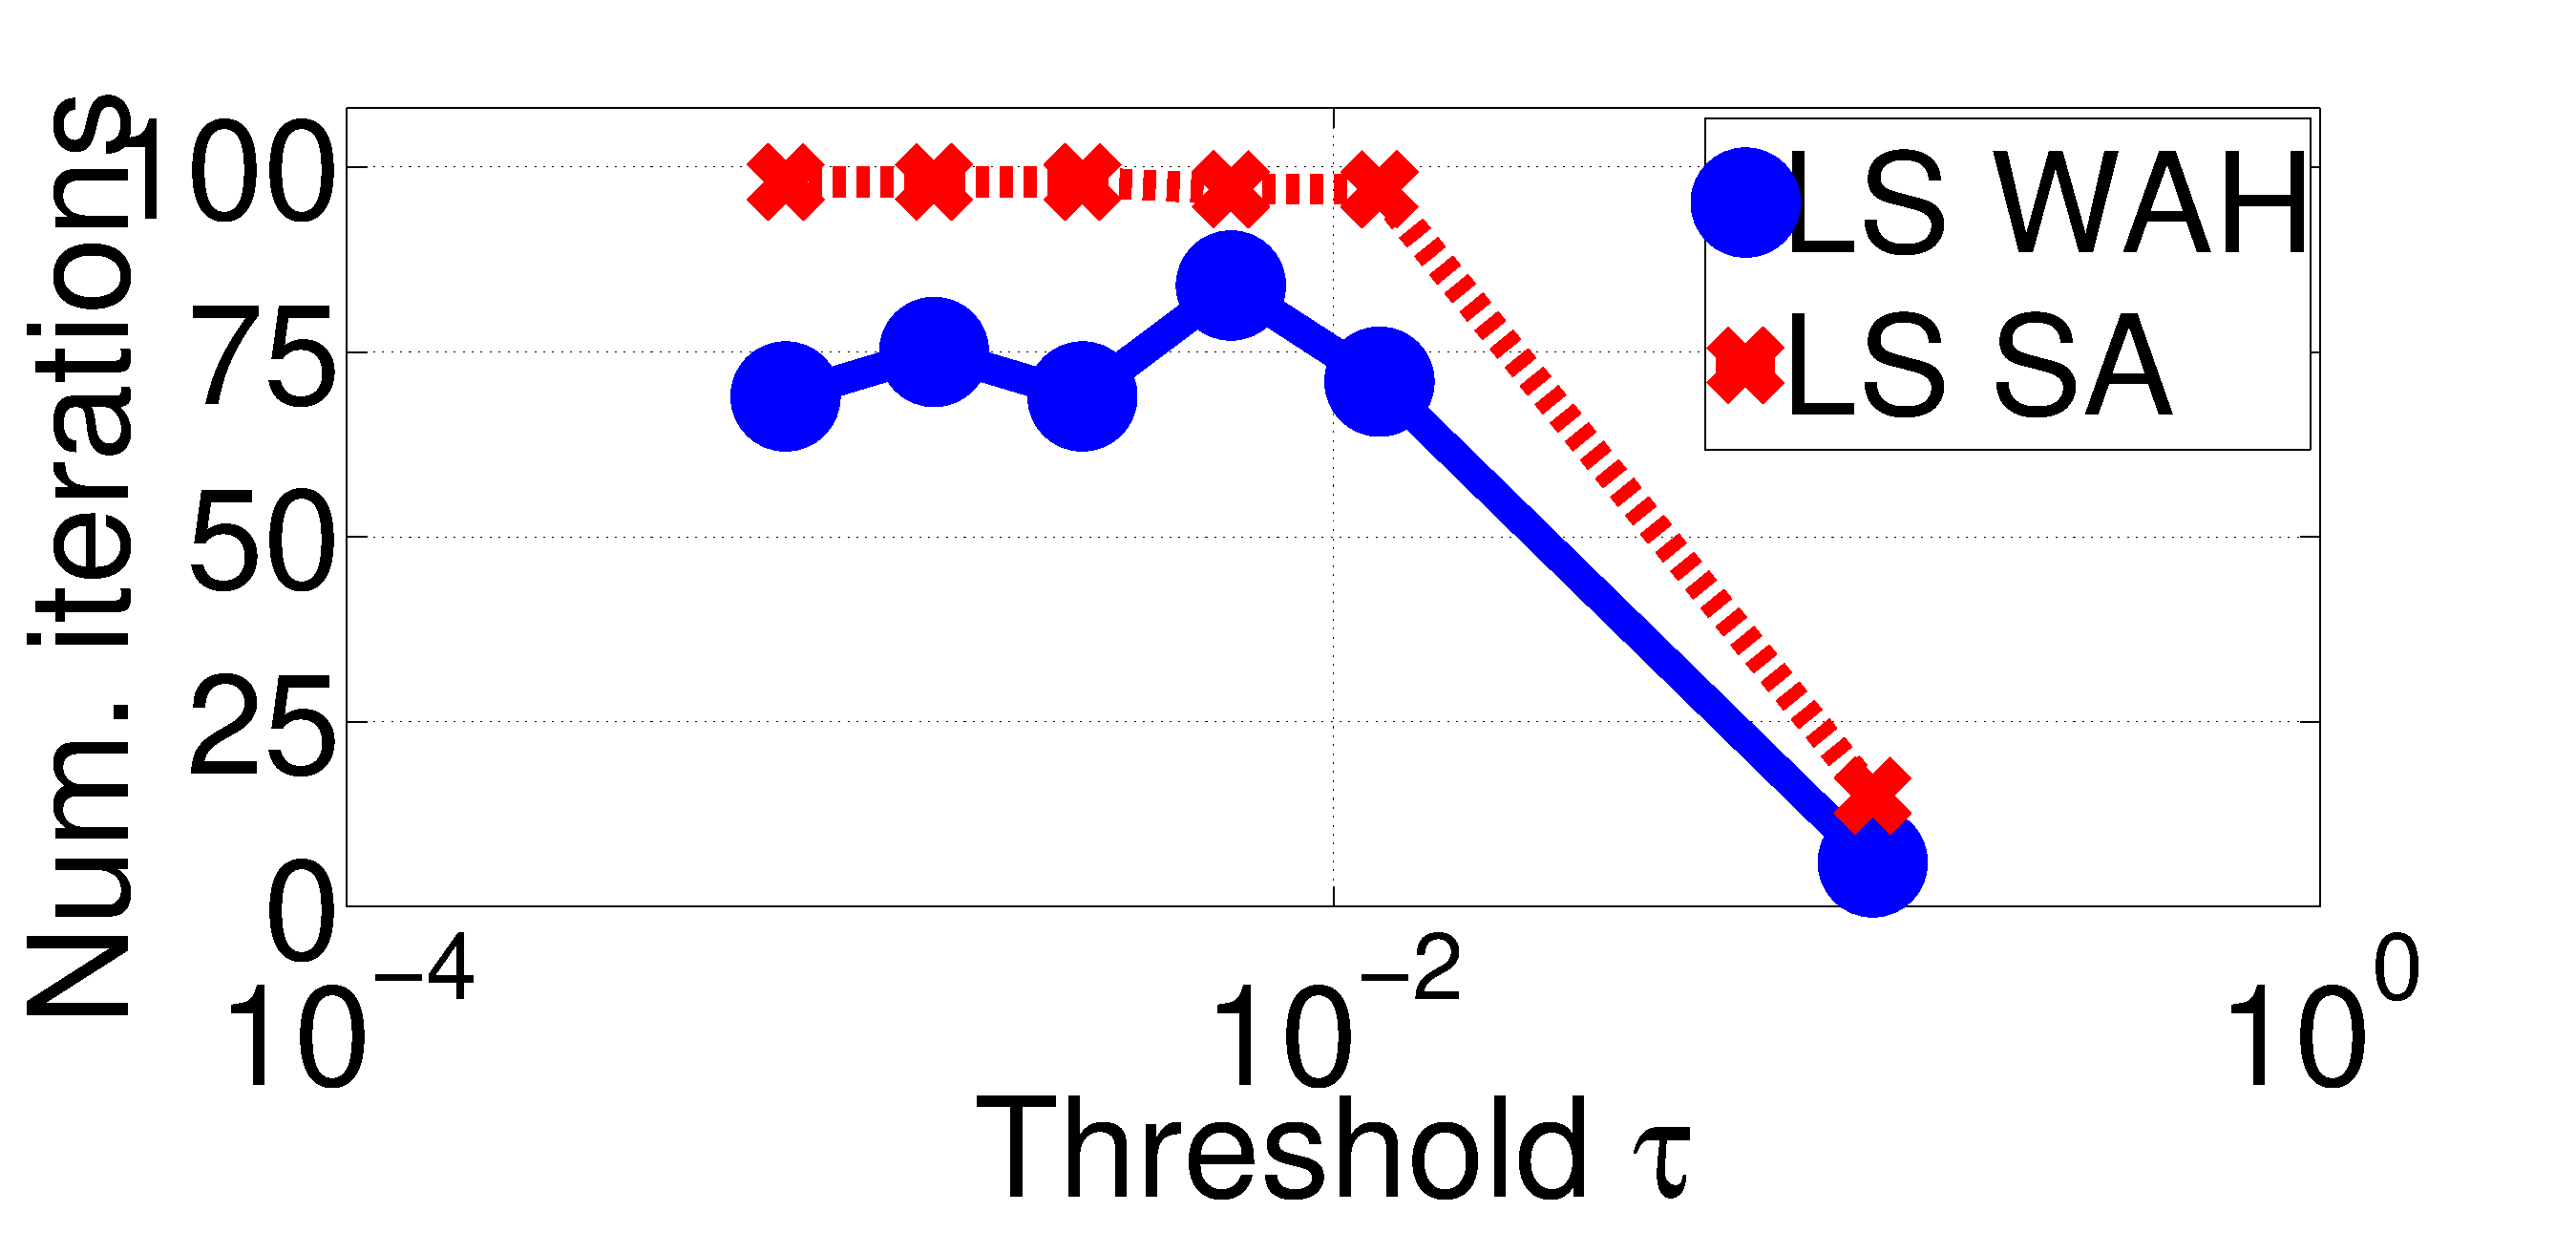
\includegraphics[width=\linewidth]{TagTree/RebuttalNIterationsWithTauNew} 
%  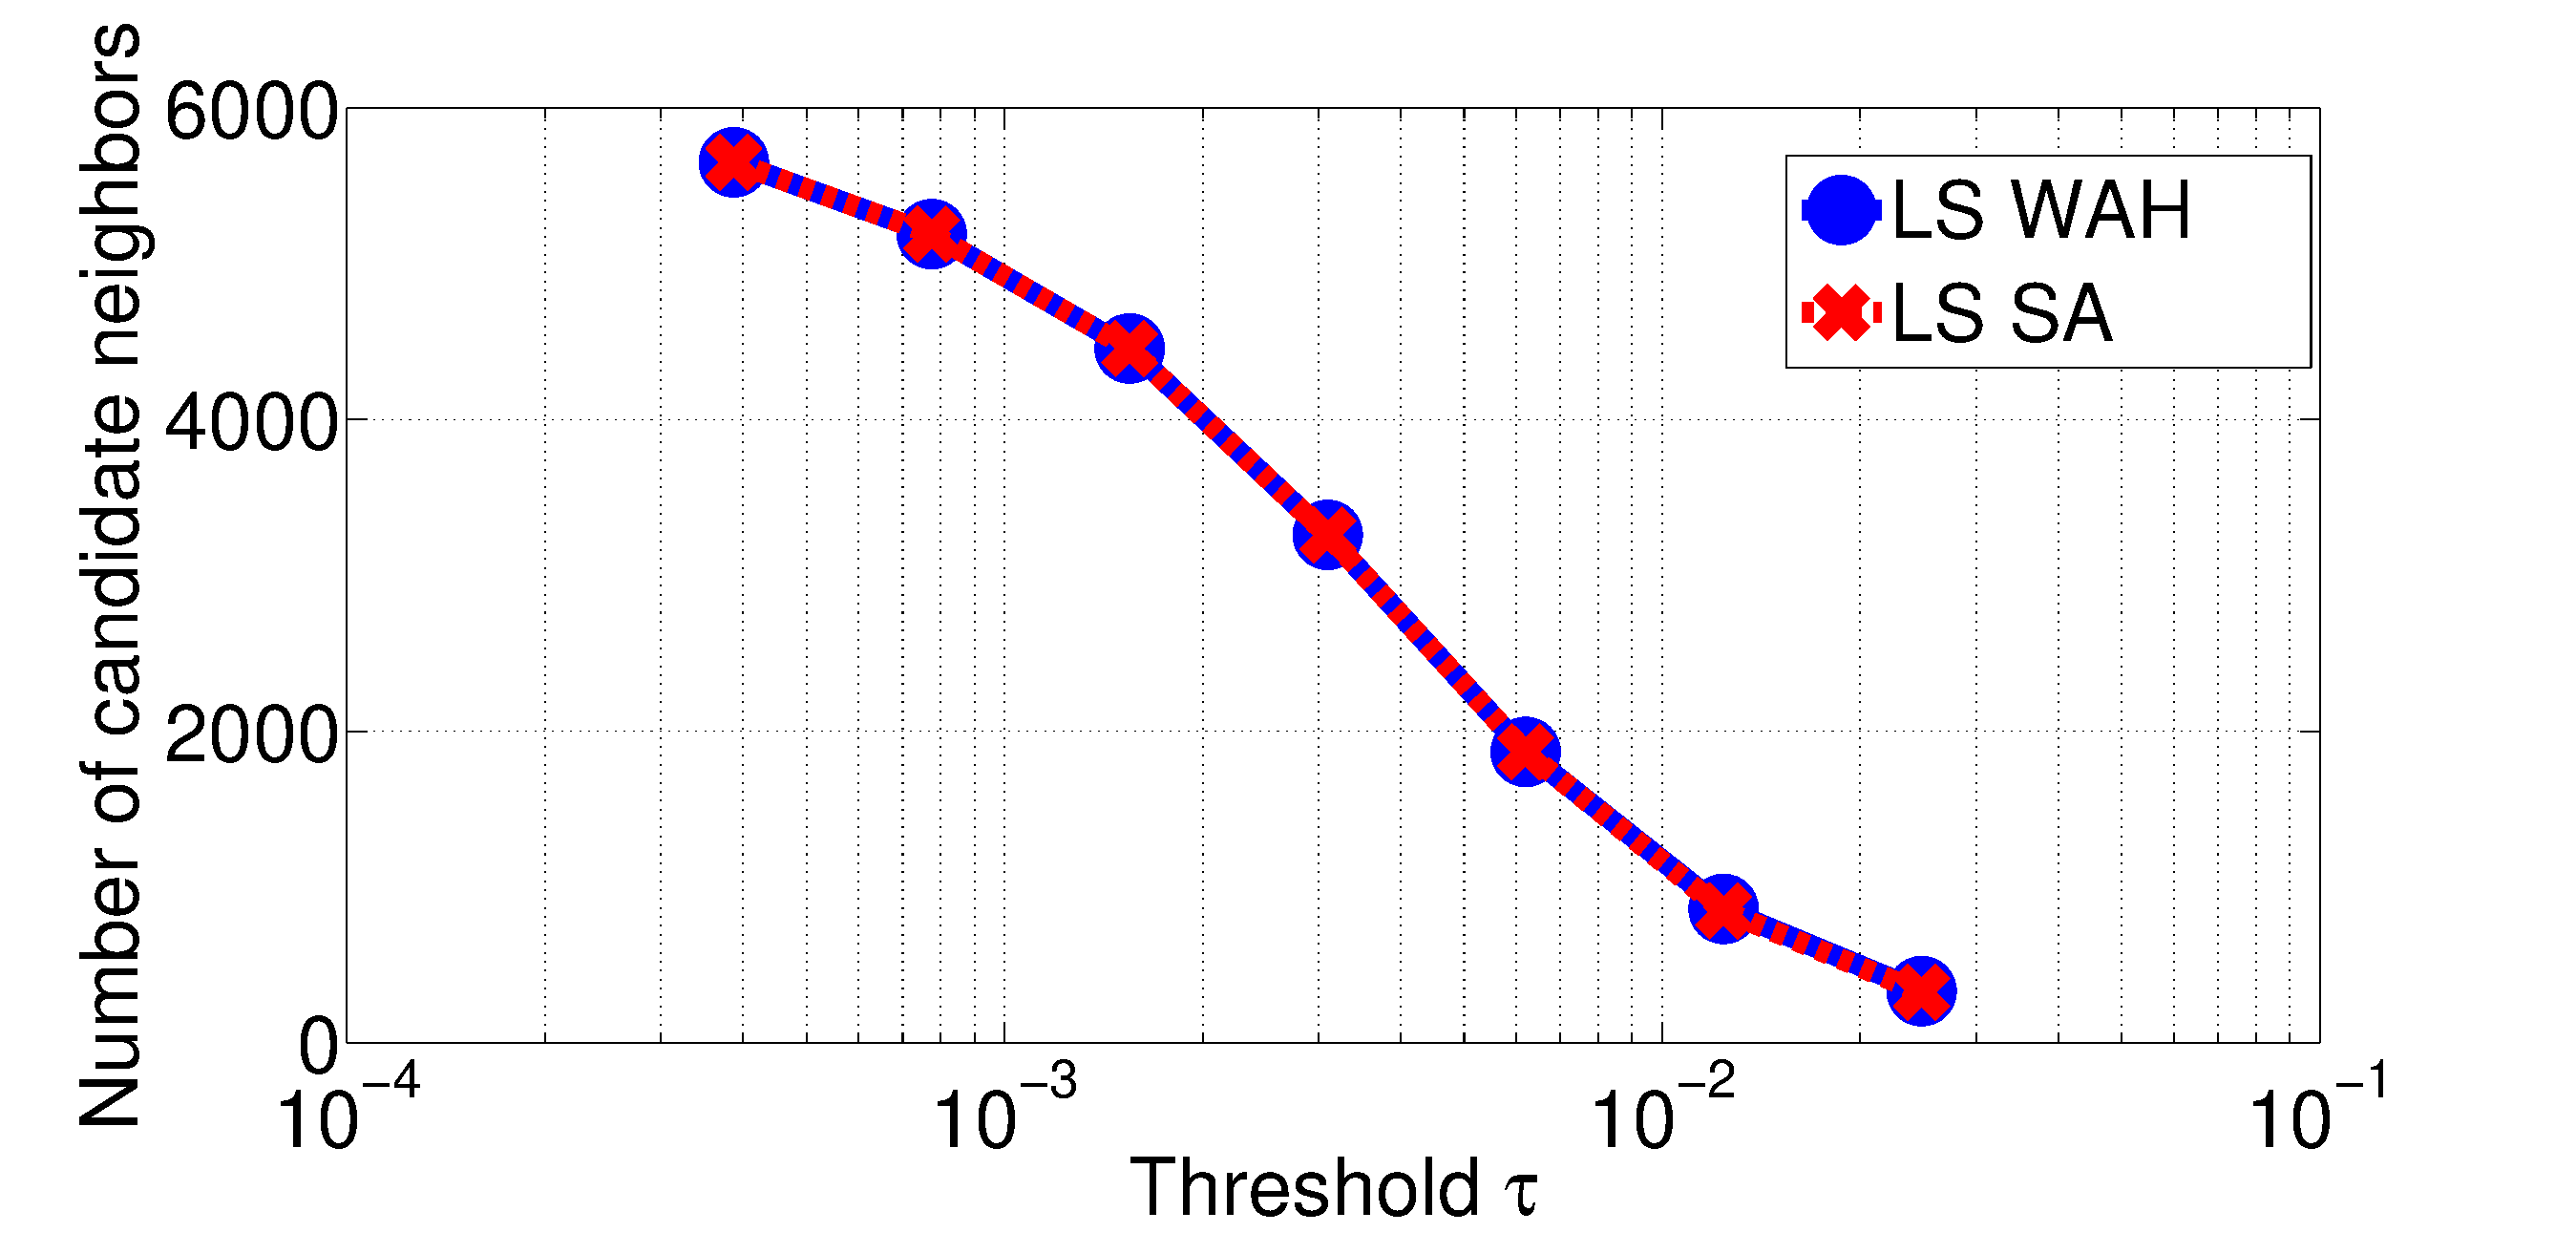
\includegraphics[width=\linewidth]{TagTree/RebuttalNCandidatesWithTau}
  \caption{Variation of number of iterations with $\tau$}
  \label{fig:TauNIterations}
%\end{centering}
\endminipage %\hfill
\minipage{0.49\textwidth}
  \includegraphics[width=\linewidth]{TagTree/RebuttalNCandidatesWithTauNew}
  \caption{Variation of number of candidate neighbors with $\tau$}
  \label{fig:TauNCandidate}
\endminipage %\hfill
\end{figure*} 
\begin{figure*}[t!]
\minipage{0.49\textwidth}
%  \includegraphics[width=\linewidth]{TagTree/RebuttalNCandidatesWithTau}
  \includegraphics[width=\linewidth]{TagTree/TimeNIterationsWithTau}
  \caption{Variation of time (hours) taken by local search to converge}
  \label{fig:TauTimetaken}
\endminipage %\hfill
%\vspace{0.1in}
\minipage{0.49\textwidth}%
  \includegraphics[width=\linewidth]{TagTree/RebuttalAccuracyWithTauNew}
%  \includegraphics[width=\linewidth]{RebuttalNCandidatesWithTau}
  \caption{Variation of the Average Tag Prediction Accuracy with $\tau$}
  \label{fig:TauAccuracy}
\endminipage
\end{figure*}

In this section, we provide a discussion on the key insights and observations made during the course of study on ontological tag trees. \\
\indent As outlined in Section~\ref{sec:ConstructionTree}, the motivation for the objective function (\ref{eq:ObjFnWeightedHops})  in the proposed approach is that in order to get a lower value for (\ref{eq:ObjFnWeightedHops}), it is more important to separate the tags $t_i$ and $t_j$ having high $J_{\mathcal{T}}(i,j)$ with less number of hops, as compared to the tags with low $J_{\mathcal{T}}(i,j)$. However, separating the latter set of tags by fewer hops would also lower the value of  (\ref{eq:ObjFnWeightedHops}). Since (\ref{eq:ObjFnWeightedHops}) attempts to minimize the weighted number of hops between tag pairs, a local search in the space of all possible trees on $\mathcal{T}$ would lead to connecting most tags to a central tag, thus forming a star graph. Such a minimum weighted hops spanning tree problem on an all connected graph can be solved in polynomial time using Gomory-Hu trees~\cite{panigrahi2008gomory}, however star graphs need not reflect the true relationship between tags in a corpus. In order to ensure that the proposed approach does not induce artificial structures because of bias of the objective function, we constrain the search space to be spanning trees of a suitably constructed Similarity Graph with the help of a threshold $\tau$, as outlined in Section~\ref{sec:refinement}. Experimentally, constraining as above does succeed in ensuring that we do not get a star graph. However upon visual inspection, the proposed approach yields star subtrees connected through their centers.
The objective function (\ref{eq:ObjFnSimApprox}) in comparison has no such bias for shorter trees and as a result, the results for proposed approach using (\ref{eq:ObjFnSimApprox}) outperform those using (\ref{eq:ObjFnWeightedHops}). 
\hl{Figures {\ref{fig:TauNIterations}} through {\ref{fig:TauAccuracy}} show the variation of different aspects of constructed tag trees with $\tau$ for 117 Flickr tags. Fig.~{\ref{fig:TauNCandidate}} shows that with increasing $\tau$, the number of tag trees that are eligible candidates in an iteration of the local search, drops drastically for both LS-WAH and LS-SA. As discussed above, a lenient $\tau$ leads to the LS-WAH based local search converging to star graphs which are an artefact of the procedure and not of the true relationships between the tags. As a result, for lower $\tau$, the performance of LS-WAH based approach degrades substantially as can be seen in Fig.~{\ref{fig:TauAccuracy}}. For large values of $\tau$, the number of candidate neighbors at each iteration of the local search become less. This constrains the local search and prevents it from attaining a lower value for the objective function ({\ref{eq:ObjFnSimApprox}}). This leads to a drop in the performance of LS-SA as can be seen in Fig.~{\ref{fig:TauAccuracy}}. We have chosen a threshold as the median of the pair-wise jaccard similarity values since it offers a convenient trade-off between number of candidates and performance for LS-SA. } 

At each iteration of the proposed approach, there are $O(N^2)$ neighbors of a tree to explore, where $N=\mid \mathcal{T} \mid$. Calculating the pair-wise distances (or hops) and computing (\ref{eq:ObjFnWeightedHops}) or (\ref{eq:ObjFnSimApprox}) requires $O(N^2)$ operations per neighbor~\cite{ford2010flows}. Thus, the complexity of the proposed approach, for either objective function, is $O(N^4)$ per iteration. \hl{A bottleneck of the proposed tag tree construction approach is the time taken for local search to terminate. Fig.~{\ref{fig:TauTimetaken}} shows the variation of the time taken by the proposed local search based approach, with respect to $\tau$. Matlab on a 2.9GHz, 8GB RAM 4 core processor is used.} One way to reduce the time taken at each iteration is to reduce the number of neighbors. This is achieved by constraining the solution space to spanning trees of a Similarity Graph. While the order of complexity at each iteration remains at $O(N^4)$, the time taken is much less. For instance, when $\tau$ is chosen as median of the pair-wise jaccard similarity values as in Section~\ref{sec:Expts}, the time taken is nearly half of the time taken when $\tau=0$, which corresponds to having search space as all possible trees on $\mathcal{T}$. 
%Thus, confining the local search to spanning trees of the Similarity Graph helps ensure that the proposed approach using objective function (\ref{eq:ObjFnWeightedHops}) gives a non-trivial solution. Since the proposed approach using objective function (\ref{eq:ObjFnSimApprox}) has no such bias 
%It is not necessary for the correctness of the proposed approach using (\ref{eq:ObjFnSimApprox}) to use the Similarity Graph.
%Thus, the Similarity Graph has different uses for objective functions (\ref{eq:ObjFnWeightedHops}) and (\ref{eq:ObjFnSimApprox}). While in the case of the former, it helps to ensure that the proposed approach leads to a non-trivial solution, in the latter case, its only use is to speed up the search for a local optimum. 
Thus, for the proposed approach using objective function (\ref{eq:ObjFnWeightedHops}), constraining the local search to spanning trees of a Similarity Graph is necessary to ensure that we do not get a trivial solution.  Doing so also makes the local search faster. \hl{As compared to this, for the proposed approach using objective function ({\ref{eq:ObjFnSimApprox}}), using a Similarity Graph only makes the optimum search faster as can be seen in the reduced number of candidates in Fig.~{\ref{fig:TauNCandidate}} and the reduced number of iterations to converge, as shown in Fig.~{\ref{fig:TauNIterations}}}. 



\hl{Intuitively, using ({\ref{eq:ObjFnSimApprox}}) as the objective function minimizes the weighted L1 norm of the difference between pair-wise jaccard similarity and the similarity estimated using a tag tree, thus trying to approximate the normalized symmetric second order statistics of a corpus using a tree on the set of tags}. We have chosen weighted L1 norm since it was observed to lead to the best results across different corpora among other variants such as L1, L2 and weighted L2 norm. Implementation of the similarity estimated using a tag tree (\ref{eq:ProdSimSimilarityCalculate}) can be conveniently done by using Logarithms and Ford Fulkerson Algorithm~\cite{ford2010flows}. Also, since the LS-SA approximates the pair-wise similarities $J_{\mathcal{T}}(i,j)$ in $O(N)$ as compared to $O(N^2)$, approaches such as {\cite{sigurbjornsson2008flickr}} that utilize $J_{\mathcal{T}}(i,j)$ lead to equal or only marginally better performance, despite having several orders higher space requirement. \\


\section{Summary}

In this section we summarize the research contributions of this chapter, key practical insights, and advantages and limitations as compared to existing expert systems. We also discuss limitations of our work, and provide several suggestions for future research directions. 

We have proposed ontological tag trees to enable expert systems address the sparsity of folksonomies effectively and in a space efficient manner. Ontological tag trees or tag trees are defined as simple trees on the set of tags in a corpus. The construction of tag trees is formulated as an optimization problem on corpus based statistics, and is solved through a novel local search based approach. We have shown that this approach can be used to build tag trees for tags obtained from two corpora, one composed of noisily annotated Flickr images and the other composed of cleanly annotated stock images. To validate the utility of the constructed ontological tag tree, we proposed two evaluation tasks involving tag prediction in images.  We have demonstrated that for the task of predicting the unseen tags of a given image with a partially observed set of tags, the proposed ontological tag trees outperform those constructed using only semantic relationships, or tag graphs constructed using commonly used techniques that have comparable space requirements. In the second task, we have shown that the tag tree obtained from the proposed approach makes the process of using appropriate classifiers to tag an untagged test image more efficient. Robustness analysis shows that the proposed approach is fairly robust to tag noise and differences between the training and test set distributions.

Compared to previous expert systems, our work offers significant advantages. In addition, several key insights can be derived from our study. Since expert systems such as~\cite{MohdSemantic13} based on only semantic relationships fail to capture the data-specific relationships between tags, their performance is significantly lower on data-driven tasks than that of ontological tag trees constructed using the proposed approach. This is demonstrated through evaluations in Section~\ref{sec:Expts}. In addition, we show that even though ontological tag trees have space requirement of only $O(N)$ for $N$ tags, as compared to $O(N^2)$ for tag graphs, tag trees can provide equal or better performance than several existing expert systems on the evaluation tasks. Particularly, compared to~\cite{sigurbjornsson2008flickr} which may require 27 terabytes of space to store pair-wise similarities, our approach requires less than 50 megabytes, and still achieves almost equal performance. Ontological tag trees can thus offer a very convenient method for expert systems to capture corpus based relationships for tasks such as tag prediction, and efficient resource classification. The significant savings in space requirement facilitates practical deployment of the expert systems even on computing devices that do not have gigantic memory available. The third key advantage of using ontological tag trees is that their construction does not depend on the availability of content-based features (such as textual or visual features). Thus as compared to previous expert systems such as~\cite{li2009learning}, \cite{wu2009distance}, \cite{HsiehCollab09}, \cite{ChenEstim15}, \cite{SunLang11}, our approach can help alleviate sparsity of online folksonomies even in domains where extracting content-based features may be inefficient or infeasible~\cite{huang2010text}, \cite{song2010taxonomic}, \cite{zanetti2008walk}, \cite{yin2009exploring}. Lastly, as discussed in Section~\ref{sec:Discussion}, the performance of the LS-SA approach is significantly better than that of the LS-WAH approach. It can thus be recommended that the LS-SA approach be used to construct ontological tag trees. 


While the proposed ontological tag trees can help expert systems achieve high performance in a space efficient manner, there are certain limitations of the proposed approach. As discussed in Section~\ref{sec:Discussion}, the time taken per iteration of the local search based tag tree construction approach varies as $O(N^4)$. For large number of tags, the total time taken to construct tag trees can be high. In addition, the tag trees only capture undirected weighted relationships between tags. As a result, any directed relationships that may be present in the corpus (for example subsumption relationships~\cite{SubsumptionFlickr}) are lost by the constructed tag trees. 


We provide several suggestions for future work directions based on our work. 
Since the tag tree construction approach has a limitation of high time requirement, one direction of future work could be to make the proposed approach faster by choosing a higher or an adaptive $\tau$, with the possible trade-off being increasing the constraint on the local search, thereby achieving a sub-optimal tag tree. Another direction of future work could be to keep a low $\tau$ but develop distributed and possibly approximated versions of the proposed approach, such that available distributed clusters, for example Amazon EC2 cloud server~\cite{AmazonEC2}, can be leveraged. 
In the current work, the LS-SA approach can be thought of as approximating the symmetric second order corpus statistics. An extension of the work could be to construct tag structures that approximate higher order corpus statistics. 
In addition, future work could utilize the constructed tag trees for other practical applications such as tag recommendation: given set of tags associated with a test images, which $additional$ tags would you associate with the image? Removal of potentially noisy tags can also be studied based on whether a tag appears too far in the tree from other tags associated with a given image. Lastly, a hierarchical taxonomy could be constructed in future, where the edges between the nodes are directed, by adopting similar techniques and using the co-occurrence data from the corpus. 

\section{Acknowledgments} 
We thank the anonymous WWW 2014 and Elsevier Expert Systems with Applications reviewers for their feedback and comments on the work. This research was partially supported by an internship at Yahoo Labs, and partially by the Center for Wireless Communications at University of California San Diego. 

Chapter 3, in part, contains material as it appears in the Proceedings of the companion publication of the 23rd International Conference on World Wide Web (WWW '14). ``Construction of Tag Ontological Graphs by Locally Minimizing Weighted Average Hops''. Chetan Verma, Vijay Mahadevan, Nikhil Rasiwasia, Gaurav Aggarwal, Ravi Kant, Alejandro Jaimes, Sujit Dey. The dissertation author was the primary investigator and author of this paper. 

Chapter 3, in part, contains material as it appears in Elsevier Expert Systems with Applications. ``Construction and Evaluation of Ontological Tag Trees''. Chetan Verma, Vijay Mahadevan, Nikhil Rasiwasia, Gaurav Aggarwal, Ravi Kant, Alejandro Jaimes, Sujit Dey. The dissertation author was the primary investigator and author of this paper. 









\chapter{Improving Scalability of Personalized Recommendation Systems for Enterprise Knowledge Workers}
The previous two chapters discussed methods that enable automatic content classification, and that address tag sparsity of annotated online content. This chapter studies a specific type of personalization system, namely a recommendation system, and shows how it can be designed for enterprise ecosystem, as well as how it can be made efficient and hence scalable. 


  Enterprise knowledge workers have been overwhelmed by the growing
  rate of incoming data in recent years.  In this chapter, we present a
  recommendation system with the goal of helping knowledge workers in
  discovering useful new content.  Specifically, our system builds
  personalized user models based on file activities on enterprise
  network file servers.  Our models use novel features that are
  derived from file metadata and user collaboration.  Through
  extensive evaluation on real world enterprise data, we demonstrate
  the effectiveness of our system with high precision and recall
  values.  Unfortunately, our experiments reveal that per-user models
  are unable to handle heavy workloads.  To address this
  limitation, we propose a novel optimization technique, Active
  Feature-based Model Selection, that predicts the user models that 
should be applied on each test file. Such a technique can reduce the 
classification time per file by as much as 23 times without sacrificing accuracy. 

  We also show how this technique can be extended to improve the
  scalability exponentially at marginal cost of prediction accuracy, e.g., we can 
 gain 169 times faster performance on average across all shares by sacrificing 4\%
  of F-score.

%% Input other tex files. Begin. %% 
\section{Introduction} 
\label{sec:introduction}
The amount of data created, replicated and consumed every year has
been growing exponentially over the
years~\cite{IDGBigDataSurvey14}.  Between 2010 and 2020, the digital
data is expected to grow by 50 times~\cite{IDCDataGrowth}.
%%
%  Since the survey was conducted last year, we cannot use below
%  sentence anymore
\comment {
The
amount of data managed by enterprises follows a similar trend and is
expected to increase by 76\% within the next 12-18 months
\cite{IDGBigDataSurvey14}.
}
%%
Following a similar trend, enterprise data was projected to
increase by 76\% within the last one and half
years~\cite{IDCDataGrowth}.  The tremendous growth of data has become one
of the biggest challenges for enterprises.  It places unreasonable
burden on enterprise users or knowledge workers.
Studies~\cite{IDGBigDataSurvey14} have shown that nearly 65\% of
knowledge workers report feeling overwhelmed by the incoming data.
The situation is further exacerbated by the fact the enterprise data
resides across heterogeneous devices and environments, including network
file servers, source control repositories, emails and file servers,
cloud applications~\cite{salesforce, office365}, and enterprise social
networks~\cite{EnterpriseSN}.  This makes finding relevant content a
very challenging task for knowledge workers.

%% Analysis of the growing data plays an
%% increasingly vital role for businesses and enterprises thus assign a
%% high priority on their ability to harness the data. At the same time,
%% the growing data places unreasonable demand on enterprise users or
%% knowledge workers to cope up with its massive volumes. Studies such as
%% \cite{IDGBigDataSurvey14} have reported that nearly 65\% of knowledge
%% workers report feeling overwhelmed by the incoming data. The situation
%% is further exacerbated by the fact that the data in enterprises is
%% stored across heterogenous devices and locations. While enterprise
%% users continue using traditional technologies such as network file
%% servers, source control repositories, emails and file servers, they
%% are also increasingly using cloud based applications
%% ~\cite{salesforce, office365} and enterprise social
%% networks~\cite{EnterpriseSN} to conduct their work. The tremendous
%% growth rate of enterprise data and the diversity in its locations make
%% finding relevant content a very challenging task for knowledge
%% workers.

In this chapter, we present a system that assists knowledge workers to
\textit{discover} relevant content by providing personalized
recommendations.  In order to serve these recommendations, our system
monitors user activity over a training period and trains per-user
access models.  Although our approach currently focuses on files on
networked file servers (shares), it could potentially be applied to other types
of data as well.  For training user models, we extract interesting
metadata features based on file path and hierarchical directory
structure.  In our experiments, we observe that many enterprise users
show a high degree of collaboration, which is inferred based on their
common file accesses.  To leverage user collaboration, we propose a
collaborative filtering aware modeling approach that provides
significant improvement over metadata-based models.  Our evaluation
uses activity logs from eight different shares of an enterprise
customer.  We measure the effectiveness of our system in providing
predictions for files that are new with respect to the training data.
Our experiments show that the metadata-based models can achieve an
average F-score of nearly 50\% at 75\% precision across all shares and users.
Our collaborative filtering-based approach remarkably improves the
same F-score to over 70\%.

Although effective, per user models are not at all efficient in terms
of the runtime performance of testing.  This is because every file
that is created or modified in a share needs to be tested against the
model of each user in the share.  This could be computationally very expensive
especially for heavy workloads with a large number of users.  For
instance, for handling a heavy workload (i.e., activity
involving high file edit rate) in our experiments, our system will
need 48 64-core machines to test all edited files.  The high computational and financial cost poses a severe
constraint that could adversely affect the adoption of our system.  To
address this issue, we propose a novel technique, called Active
Features-based Model Selection (AFMS), that automatically selects only
those user models that are highly likely to generate positive
predictions, while ignoring the models that will definitely or most likely generate
negative predictions.  Thus using this technique, a test file is
tested against only the selected models, thereby speeding up the
overall testing time.  Our experiments show that AFMS drastically
reduces testing time without any loss in the prediction accuracy.
Furthermore, we show that AFMS can be used adaptively to trade-off
marginal prediction accuracy for significant performance gains during
the periods of heavy workload.


Our previous version~\cite{dwiticeis15} of this work presented the
basic technique for modeling file accesses.  This chapter presents a
new technique, AFMS, for improving solubility, along with new
experiments and insights.  The main contributions of our work are the
following:
\begin{enumerate}
\item Propose a system to analyze user file accesses in order to train
  personalized models, and recommend relevant content with a high
  degree of accuracy
\item Propose a novel model selection technique that can speed up the
  testing time by more than 6 times on average, and by over 23 times in the best case
  without any loss in the prediction accuracy
\item Extend the model selection technique to speed up the testing time
  significantly at the cost of marginal loss in the prediction accuracy
\item Demonstrate practicality of our system using a systematic study
  and evaluation based on real world enterprise data
\end{enumerate}

%%
%%  The justification for 24 64-core machines needed
%%  What is the constriant un latency of prediction?
%%
%% In this paper we present a system that assists knowledge workers to \textit{discover} relevant content by providing personalized
%% recommendations. In order to serve the recommendations, our system
%% monitors user activity over a training period and trains per user
%% access models. We focus on files on networked file servers and use a novel tokenization approach to extract metadata based features from files that enable the training of user models. In addition to modeling user access patterns using the file metadata, we note that enterprise users demonstrate a high degree of collaboration with respect to
%% common files. Thus we also propose a collaborative filtering aware modeling approach that can leverage the user collaboration and can improve the performance of our system over that of metadata based models. 
%% We provide evaluation of the system by using activity logs from eight shares of an enterprise customer. Since the system is designed to recommend new content to users, we ensure that the test data comprises of files that are new with respect to the training data. Our experiments reveal that the metadata based models can achieve average F-score of over 90\% and average recall of over 93\% for 75\% precision. In addition, user collaboration in enterprise shares can be leveraged to get average F score of over 99\% and average recall of over 99\% for 75\% precision. 
%
%In particular, the system is designed for files on networked file servers. File servers are used by enterprises for several purposes such as storing application specific data, facilitating collaboration among users, backing up data, and hosting personal home directories. 
%
%
%
%
%In addition to improving productivity of enterprise users, the proposed system can also be used to determine which files to cache on mobile devices in scenarios of intermittent connectivity. Alternatively, it can be used to reduce network latency in cloud services by caching files on client-facing web servers or directly on clients.


%% While the evaluation demonstrates feasibility of using our system to provide recommendations with high predictive correctness, the per user modeling used in our system inhibits its scalability to large shares. Specifically, for every created or modified file in a share, the models corresponding to each user in the share need to be applied. As a result of this, the computational requirement during testing can be substantial. As an example, for a populated share experiencing high file edit rate, our system may need 24 64-core machines on average for testing. This places severe computational and financial requirements on enterprises that adopt our system to help its knowledge workers discover relevant content and may even make deploying our system infeasible for large shares. 

%Practical insights are provided relating the system performance with training duration for models, separation between training and testing and user workload.
%While existing file access prediction approaches such as \cite{yeh01-mascots,yeh01-ispass} fail to provide predictions for new files, 
%The system, however, necessiates that models are constructed for each user in a share be applied on a created or modified file. As a result, classifying a file has high computational requirement which may prevent our system from scaling to large and active shares. 

%% In order to reduce the high testing computational requirement of our system, we propose a novel Active Features based Model Selection (AFMS) approach that can \textit{select} user models that may recommend a given test file to their corresponding users. Based on this, only the selected models need to be applied on the file, thus reducing its testing time computational requirement. 
%% We show empirically and verify through experiments that AFMS can reduce the computation per file testing by more
%% than an order of magnitude without any loss in model correctness. In
%% addition, we demonstrate that AFMS can reduce the testing complexity by more than two
%% orders of magnitude with graceful degradation in model
%% correctness. Furthermore, AFMS can also enable adaptive techniques that can trade off model perdictive correctness for faster processing of files during periods of high file activity in shares. Based on the proposed approach, we show that our system can be
%% scaled up to shares accessed by large number of users and having high rates of file activity, and can be implemented using only a household machine. 

%% \cite{dwiticeis15} presents a previous version of this work. The
%% current paper presents new techniques, extensive new
%% experiments and insights as compared to \cite{dwiticeis15}. The main
%% contributions of our work are the following: 
%% \begin{enumerate}
%% \item Propose a system to analyze user file accesses to train
%%   personalized models and recommend relevant content
%% \item Propose a novel model selection approach that
%%   can reduce the high computational requirement of the system by 5 times on average and by over 20 times at maximum without any loss in predictive correctness 
%% \item Propose an approach that can lower the testing computational requirement by several orders at the cost of marginal loss in the model predictive correctness
%% \item Demonstrate viability of proposed approaches using a systematic study and evaluation based on real world enterprise data 
%% \end{enumerate}


\comment{
Rest of the paper is organized as follows.  \\ 
\textbf{pending} \\ 
\textbf{Need to draft differences with ICEIS paper too.}\\ 
}
%%%% OLD CONTENT: COMMENTING %%%
\comment{ 
Enterprise knowledge workers are inundated with new options for
conducting their work with the rise of Enterprise Social
Networks~\cite{EnterpriseSN} and cloud based
applications~\cite{salesforce, office365} alongside traditional
technologies such as email, source control repositories, network file
servers, and office software suites.  Enterprises are also embracing
new computing devices such as mobile devices and tablets in addition
to existing personal computers, laptops, workstations and servers.
The amount of enterprise data grows significantly each year: studies
estimate that unstructured data grows annually by
40-50\%~\cite{IDCDataGrowth}.  The fragmentation in the tools and
devices used to work and the sheer growth of data places increasingly
unrealistic demands on knowledge workers to keep up with the influx of
data.  In fact, it has been reported that 65\% of users have felt at
times overwhelmed by the amount of incoming
data~\cite{IDGBigDataSurvey14}.

This chapter presents a system that utilizes machine learning and
natural language processing to automate the discovery of important new
or modified content and identify which subset of users will likely use
or benefit from it. The system is designed for file servers
and is evaluated with activity collected over eight network file
servers from an enterprise customer.  Enterprises use file servers for
a myriad of purposes including storing application data, back up,
enabling collaboration, and hosting personal home directories. The
proposed system will support a wide range of applications, such as
recommender systems or server cache management systems, by providing
predictions about what data will likely be accessed in the near
future.

The system bases its predictions on user activity and content
metadata.  We track content accessed by users over a specified
training interval.  Data (i.e. access to a particular piece of
content) are represented by a set of features that include path
components (e.g., parent and ancestral directories), keywords in the
path, and extension.
% NB - if we remove tokenization details, we should remove this sentence
%We employ a novel tokenization scheme to extract salient keywords from the
%metadata because it is common to observe concatenation and uniform case in
%naming files and folders.  
Each datum represents an instance in training our model.  Combining
this training data with the files specifically accessed by the user,
this system builds personalized models to predict future file
accesses. While traditional approaches for file access prediction such
as \cite{yeh01-mascots,yeh01-ispass} cannot be applied to recommend
new files, the proposed user model based approach is generalizable
enough to be applied even to content that has not been accessed
before, or is newly created. Additionally, analysis of file activity
yields the insight that very regular patterns of collaboration occur.
The chapter demonstrates a method in which an individual's prediction
precision and recall can be greatly improved by incorporating the
predictions of all other user models.

This work makes the following contributions:
\begin{itemize}
\item Observations about the nature of enterprise file activity
\item A system that analyzes file activity and metadata and applies
  machine learning and natural language processing to provide
  predictions
%\item A method to tokenize file metadata
\item A strategy to combine the personalized models of multiple file
  users to improve the predictions of individual users
\end{itemize}
%The paper is organized as follows.  Section~\ref{sec:data} provides observations
%about file activity data. Section~\ref{sec:features} details the feature space
%and Section~\ref{sec:models} details the approach to construct and evaluate
%individual models. Section~\ref{sec:evaluation} evaluates the performance of
%this model with discussion in Section~\ref{sec:discussion}.  These sections are
%followed by related work in Section~\ref{sec:relatedwork} and a conclusion in
%Section~\ref{sec:conclusion}.

%% Redundant with first highlight - MAH
%% We evaluate the proposed approach over activity data recorded on
%%   ten network file servers activity data from an enterprise customer.  in the shares corresponds to
%%   real world data from enterprises. 

The chapter is organized as follows. 
  Section 2 provides observations about file activity and pre-processing.
  Section 3 details the feature space and
  Section 4 describes the construction of metadata and collaborative filtering-based user models.
  Section 5 presents an evaluation of the user models and 
  Section 6 discusses the contributions and characteristics of the features used
  in the models, and scalability and deployment related aspects. 
  Section 7 identifies related work followed by a discussion on directions for future work in Section 8. Section 9 concludes. 
}
%%%% OLD CONTENT: COMMENTING %%%  

\section{The File Recommendation System}
\label{sec:overallsystem}
\begin{figure}
\centering
{\fontsize{8pt}{1em}\selectfont
\begin{tabular}{c}
\includegraphics[trim = 0mm 0mm 0mm 4mm, clip, width=0.65\linewidth]{FileAccess/figs/meta_training} \\
\multicolumn{1}{l}{(a) \textbf{Training}: metadata models for each user} \\ 
\includegraphics[trim = 0mm 0mm 0mm 7mm, clip, width=0.65\linewidth]{FileAccess/figs/testing} \\
\multicolumn{1}{l}{(b) \textbf{Testing}: apply the trained models for all users in share} \\  
\includegraphics[width=0.62\linewidth]{FileAccess/figs/cf_training2} \\
\multicolumn{1}{l}{(c) \textbf{Training}: CF models for each user} \\  
\end{tabular}
}
\caption{Approach Overview}
\label{fig:overallfigs}
%\vspace{-0.5cm}
\end{figure}

%%
Our system uses a binary classification approach for providing file
recommendations.  For this purpose, it builds a separate
classification model for each user of a file share.  The dataset of a
given user includes all the files that have been accessed by all 
users of the share.  The label of a file in the dataset is $1$ if the
user accesses it, $0$ otherwise.  It is important to know that if a
user accesses a particular file during the training phase, it is
highly likely that the user will access the same file during the
testing phase.  Recommending such a file to the user is not very
useful.  Hence the main objective of our system is to discover useful
but new files that may have been created or modified by other users of
the same share.  For this reason, the testing phase includes only
those files that are new with respect to the training phase for the
user.  Our system then applies the model of the user to these files to
predict classification labels.  The rest of this section describes the
features and the modeling techniques used in the system.

%% The proposed system comprises of a training and a testing
%% phase. During training, file activities are monitored, features are
%% extracted from file metadata and a model per user is trained. This is shown
%% for metadata based models in Figure~\ref{fig:overallfigs}(a). During testing or classification phase (Figure~\ref{fig:overallfigs}(b)), features are
%% extracted from each created or modified file and the trained models for
%% every user in the share are applied on the file. The features used and modeling
%% techniques adopted are briefly described below.

%Details can be obtained from~\cite{dwiticeis15}. 
\subsection{Metadata Features}
\label{sec:features}
%%
The metadata features include features extracted from different
attributes of a file:
%% The metadata features of each training or test file are concatenation
%% of its folder, token and extension features.
%%
\begin{itemize}
  \renewcommand{\labelitemi}{$\bullet$}
%%
\item \textbf{Folder}:
%%
We create a folder feature corresponding to every folder and its
ancestor folders observed in the training period\footnote{Please note
  that no features are derived for completely new attributes seen only
  during the testing phase.}.  For a file $f$, we capture the folder
features as a binary vector with the value 1 in the locations
corresponding to the folder or the ancestor folders of $f$, and 0
elsewhere.  These features help in learning a user's preference for
certain subtrees of the file system hierarchy in a share without
having to define a folder distance metric.
%%
\item \textbf{Token}:
%%
We tokenize the path name of each file using a novel tokenization
approach, the details of which can be found in~\cite{dwiticeis15}.  We
construct a token vocabulary using all the tokens observed during the
training phase.  For extracting features, we capture tokens of a file
as bag-of-words representation on the entire vocabulary.
%%
\item \textbf{Extension}:
%%
We construct an extension vocabulary based on the popular extensions
observed in the training data.  We then use this vocabulary to
represent a file's extension with one-hot encoding-based features.
%%
\end{itemize}
%%
%% \begin{enumerate}
%% \item \textbf{Folder features}: We create a folder feature
%%   corresponding to every folder and its ancentor folders observed in
%%   the training period. For every training or test file $f$, its folder
%%   features are a binary vector with 1 in locations corresponding to
%%   the folder of $f$ or its ancenstors, and 0 elsewhere. This feature helps learning a user's
%% preferences for certain subtrees of the file system
%%   hierarchy in a share without the need of definining folder distance
%%   metrics.
%%
%% \item \textbf{Token features}: We tokenize the path name of each file using a novel tokenization approach, the details of which are given in ~\cite{dwiticeis15}. The tokens resulting observed during training are used to construct a token vocabulary. The tokens in each file's path are represented using bag of words representation on the constructed vocabulary. 

%% \item \textbf{Extension features}: We construct an extension vocabulary based on the popular extensions observed in the training data. One-hot encoding is
%%   used to represent the extension of each file based on the constructed extension vocabulary. 
%% \end{enumerate}
%The metadata features of a file are concatenation of its folder, token and extension features. 

\subsection{Modeling Techniques} 
\label{sec:Metamodels}
%%
We first build basic metadata models based on the metadata features.
Using these models, we then develop an innovative approach to leverage
collaboration among users for building collaborative filtering aware
models that provide better performance over the basic metadata models.
%% Our system trains per user models using the activity observed over a
%% training period. For user $u$, every file $f$ that has been read in
%% the training period is a training instance. The corresponding label is
%% 1 if $u$ has read $f$ during training, 0 otherwise. Thus while the
%% training instances for all users in a share are the same, the labels
%% may be different. For testing, every file that has been read in
%% testing period and has $not$ been seen in training is a testing
%% instance. Doing so ensures that the models are evaluated over files
%% that are new with respect to the training data. Testing labels are
%% determined in a similar manner as training labels. We approach file
%% recommendation as a classification problem and use the following
%% modeling approaches.
%Below are the two modeling aproaches used in our system. 

\subsubsection{Metadata-based Modeling}
%%
For each user, we train a metadata model using the metadata features.
Figure~\ref{fig:overallfigs} (a, b) shows the training and the testing
phases of this approach.  Considering the trade-off between accuracy
and training time efficiency~\cite{dwiticeis15}, we pick Support
Vector Machine (SVM) with a linear kernel as our modeling technique
because it provides high accuracy without incurring significant
training time.  More importantly, a linear SVM provides feature
weights that capture the relative significance of individual features.
We leverage this aspect in our scalability optimization technique AFMS
as described in Section~\ref{sec:testspeedup}.

%% For each user, we train a metadata based model using the metadata features of the training files and their labels. We have chosen Support Vector Machines (SVMs) with linear kernel as the models since they offer high accuracy without
%% incurring significant training time. \cite{dwiticeis15} provides a
%% comparison between different machine learning models. 
%% In addition, linear SVMs provide feature weights that can determine the significance of individual features, and can be leveraged for techniques such as Active Feature based Model Selection (Section~\ref{sec:testspeedup}) to improve the scalability of our system. 
%% The training and
%% testing for metadata based models is shown in
%% Figures~\ref{fig:overallfigs}(a) and \ref{fig:overallfigs}(b)
%% respectively.
\subsubsection{Collaborative Filtering (CF)-based Modeling} 
\label{sec:CFdetails}
%%
Enterprise users often show a high degree of collaboration in terms of
accessing common files in a share.  We make this observation based on
the measurement of the metric, \textit{normalized triangle count} 
(Section~\ref{sec:data}), that captures the degree of collaboration
among users.  As an illustration, see Figure~\ref{fig:snagraphs} that
shows user communities in terms of social network graphs for a couple
of shares.

We leverage user collaborations to build CF models that are
significantly more effective than the metadata models.  Here are the
details of the method used in building a CF model for a user $u$.
First, we divide the original training set into a new training set and a
validation set.  We then use the new training set to train a metadata
model for each user.  Second, for each file in the validation set, we
apply the metadata models of all the users, and generate a vector of
the resulting predicted labels.  Third, we train the CF model for the
user $u$ using the files in the validation set.  For this, we
construct the feature vector for each validation file by concatenating
the metadata features with the vector of the predicted labels
(Figure~\ref{fig:overallfigs}(c)).  For each test file observed during
the testing phase, we first apply the metadata models of all the users
to generate a vector of the predicted labels.  Finally, we append this
vector to the metadata features to create a new feature vector and
feed it to the user $u$'s CF model to obtain the final predicted
label.


An interesting point to be noted here is that our CF-based modeling
technique does not require a pre-defined user-user relationship or
even a user similarity metric.  Rather, the model can automatically learn
positive or negative correlation between the activities of users, and
accordingly adapt to make better predictions.  For instance, if two
users have similar access patterns, the CF model for one user could
learn that its labels positively correlate with labels predicted by
the other user's metadata model.  Thus, greater the degree of
collaboration, the better will be the effectiveness of the CF models.
Another benefit of our technique is that, unlike pure collaborative
filtering-based systems developed in the past, it does not suffer from
a cold-start problem.  Previous systems recommend an item to a user if
other \textit{similar} users have shown a preference for that item.
Therefore, these systems are incapable of recommending a completely
new item because no other user has seen it before.  In contrast, the
novelty of our technique is in using CF features that are based on
predicted labels rather than the history of past accesses.

%% Enterprise users demonstrate a high degree of collaboration in terms
%% of accessing common files in a share. This is validated in Section~\ref{sec:data} where we measure the collaboration among users in terms of normalized triangle counts and also demonstrate the existence of user communities in social network graphs for sample shares. For each user, we train a CF aware model that captures the
%% predictions of all metadata based user models in a share with the aim of making
%% better prediction for the user by leveraging user
%% collaboration. In order to do this, we divide the set of training files into training and validation files. The metadata based models corresponding to each user in a share are trained on the training files and each
%% metadata model is applied on each validation files, resulting
%% in a vector of predicted metadata model based labels per validation file. 
%% The CF aware model for each user is then trained using all validation files. The features used for each validation file are concatenation of its metadata features, and the vector of predicted metadata model based labels for the file. This is shown in
%% Figure~\ref{fig:overallfigs}(c). On a test file, first the metadata
%% based models of all users in a share are applied to obtain the
%% predicted metadata model based labels. They are then concatenated with the file's metadata
%% features and the CF aware models are then applied to obtain the final predicted label for the user.
%% %Such an approach enables capturing the relationships between predictions of different users in a share. 

%% The CF aware modeling as proposed above does not require a pre-defined user-user relationship or even a similarity metric. Rather, the model can automatically learn if there is positive or negative correlation between the activities of users, and accordingly adapt the model to use this information to make better predictions. For example if two users have similar access patterns, then the CF aware model for one user could learn that its labels typically correlate with labels predicted by the other user's metadata based model. It is expected that CF aware models can provide most benefit in a share that demonstrates substantial user collaboration. 
%% Another benefit of using the above approach is that unlike purely collaborative filtering based systems, the proposed approach does not suffer from cold-start problem. Systems that recommend items to a user if other \textit{similar} users have liked, accessed or purchased the item are incapable of recommending items that are completely new since there are no users who have already accessed it. As compared to these, the collaboration based features that are utilized in the CF aware models are based on \textit{predicted} labels instead of actual past accesses and are used in addition to metadata features. 


\section{Evaluation Framework}
\label{sec:evaluation}
%%
This section describes the evaluation data and methodology.
%% This section describes the data used and the experimental methodology adopted for evaluating the proposed file recommendation system. 

\subsection{Data}
\label{sec:data}
\begin{table*}[!htpb]
\centering
{\fontsize{8pt}{1em}\selectfont
%\begin{tabular}{|p{0.5cm}|p{1.28cm}|r|p{1.15cm}|p{1.1cm}|p{1.4cm}|}
  %\begin{tabular}{|>{\centering}p{0.8cm}|r|r|>{\centering}p{2.7cm}|>{\centering}p{2.3cm}|r|}
\begin{tabular}{|>{\centering}p{0.8cm}|r|r|r|r|r|}
\hline
%Share & Sample period (days) & Users & Files operated on & Total file operations &Norm. Triangle Count \\
\textbf{Share} & \textbf{\# days} & \textbf{\# users} & \textbf{\# files operated on} & \textbf{\# file operations} &\textbf{Norm. Triangle Count} \\
\hline
A & 123 & 992 & 36,009 & 11M &  8K \\ \hline
B & 122 & 464 & 1,309 & 136K &3K \\ \hline%Correction made to camera ready
C & 122 & 160 & 1,044,779 & 3M &  $<$0.1\\ \hline
D & 121 & 183 & 746 & 11K & 951\\ \hline%Correction made to camera ready
E & 66 &  1,288 & 99,733 & 292K &3K \\ \hline
F & 66 & 937 & 6,911 & 4M &0.4 \\ \hline
G & 66 & 198 & 334 & 14K  & 3K \\ \hline
H & 57 & 398 & 133,006 & 4M  &45\\  \hline
\end{tabular}
\caption{Statistics of shares used for evaluation 
} 
\label{tab:datasetstats1}
}
\end{table*}

%%
\begin{figure*}[!htbp]
\centering
\begin{tabular}{cc}
\centering
\includegraphics[trim = 0 4cm 2mm 5cm, clip, width=0.45\linewidth]{FileAccess/figs/6261_jacc_pt5}
& 
\includegraphics[trim = 2mm 4cm 7mm 5cm, clip, width=0.46\linewidth]{FileAccess/figs/6216_jacc_pt5} \\ 
(a) Share B & (b) Share D \\ 
\end{tabular}
%%
\caption{Social network graphs for shares show that users collaborate
  and tend to form communities by accessing common files.  In these
  graphs, each node corresponds to a user, and an edge connects two users
  when the Jaccard index of common files accessed by those users is
  above $0.5$.}
%%
\label{fig:snagraphs}
\end{figure*}
We use file activity logs from eight network file shares of an
enterprise customer for evaluation.  Table~\ref{tab:datasetstats1}
provides key statistics of this data.  Because our recommendation
system targets user collaborations, we select shares from
90\textsuperscript{th} percentile in terms of triangle count -- a
metric to capture degree of collaboration among users.  Triangle count
for a share is the number of triangles formed, where a triangle edge
corresponds to a connection between two users based on accessing at
least one common file.  The table shows the triangle count values
normalized with respect the number of files.  For better
visualization, see Figure~\ref{fig:snagraphs} that shows users forming
different communities based on their collaborations. \\

%% We use the activity log data from eight network file servers (shares) of an enterprise customer for evaluation.
%% %The reader is directed to \cite{dwiticeis15} for details on workload statistics and popular files in these shares. 
%% The selected shares fall in the 90\textsuperscript{th} percentile in
%% terms of total number of triangle counts, i.e., number of triangles
%% formed when two users are connected if there exists at least one file
%% that both users have accessed. Table~\ref{tab:datasetstats1} captures
%% their key statistics. We measure the collaboration among users in a share based on the triangle counts normalized with respect to the number
%% of files. Figures~\ref{fig:snagraphs}(a) and (b) show the social
%% network graphs for users in two shares. It can be seen that the users tend to
%% form communities by co-accessing files.

\noindent\textbf{Removal of automated activity}: 
\label{sec:removebursts}
%%
We observe two types of file activities in our data.  The first
corresponds to the activities that are manually initiated by
users. These activities are characterized by a low number of file
operations per hour.  The second corresponds to scripted activities
that are performed by automated computer programs or scripts.  These
activities are generally seen as bursts or exceptionally high number
of file operations per hour.  Since our goal is to assist knowledge
workers and not automated programs, we need to remove the scripted
activity from the evaluation data.  For this purpose, we remove
the activities by a user in an hours if the number of activities are 
determined to be exceptionally high. Towards this, an appropriate threshold 
is determined using Tukey's outlier
factor~\cite{wang2011statistical}.\linebreak

%% We note from our data that user file activities typically constitute of two modes of operation. The first corresponds to users deliberately performing an action in the file system and is characterized by low number of file operations per hour. The second mode corresponds to scripted activity performed by computer programs or scripts and is seen as bursts or exceptionally high number of file operations per hour. Since our system is designed to assist knowledge workers and not automated computer programs operating from their accounts, the scripted activity should be removed from the evaluation data. We approach this as an anomaly detection problem and argue that if a user is seen to make a high number of file operations per hours, then a large fraction of the actions were scripted. We use Tukey's outlier factor~\cite{wang2011statistical} to determine an appropriate threshold on the number of activities per user per hour. The activity by a user in an hour is labeled scripted and removed if the number of file operations by the user in the hour are above the calculated threshold. 
%% %In order to avoid discarding actual user activity, the threshold is empirically set to 1000 which is above the threshold calculated using~\cite{wang2011statistical}. If a user is seen as making more than 1000 file operations per hour, then a large fractions of the actions were scripted. 
%% The data obtained after removal of scripted activity is used for the rest of the paper. 

\noindent\textbf{Selection of evaluation users}: 
\label{sec:selectusers} 
%
Since our system helps users discover new or modified content, it is
primarily targeted for active users.  Therefore, for each share, we
sample 30 users from the highest quartile of users in terms of number
of activities, and use them in our evaluation.
%% Since our system helps users discover new or modified content, it is most useful for active users. Thus for each evaluation share, we sample 30 users from the highest quartile of users in terms of number of activities, and use them to evaluate our system. 
%
\subsection{Evaluation Methodology}
\label{evalmethodology}
%%
We experiment with different training and testing periods to evaluate the
performance of our system under different settings. 

%%
%Per user models are trained over the training period and tested on actual user activities in the testing period. Experiments are conducted by varying the training and testing periods as described below. 

%% We experiment with different training and testing periods to study the performance of our system under different settings. 
%% %Per user models are trained over the training period and tested on actual user activities in the testing period. Experiments are conducted by varying the training and testing periods as described below. 

\subsubsection{Varying training and test periods} 
\label{sec:varytraintest} 
\begin{figure}[!htbp]
\begin{center}
\centering
\includegraphics[width=0.75\linewidth]{FileAccess/figs/traintestsplits}
\caption{Splitting dataset into various training and testing periods
%The training period is used for feature extraction and model
%training, and the testing period is used for evaluation of the
%trained models.
} 
\label{fig:traintestsplits}
\end{center}
\end{figure}
%%
We divide the total duration of data from each share into several
slices and create training and testing periods such that testing
occurs immediately after training. For consistency, each share is
divided into seven slices and five training and five testing periods
are created as shown in Figure~\ref{fig:traintestsplits}.
We perform experiments with different combinations:
\begin{itemize}
  \renewcommand{\labelitemi}{$\bullet$}
\item\textbf{Fix testing, vary training.}  A longer training window has
  more number of activities, thereby allowing better model training. 
 However the activities become older as the
  distance between them and the testing period increases, thus preventing the model from reflecting the latest user patterns accurately.  On the
  other hand, a small training window has less number of activities,
  but these activities are relatively fresh.  Thus, there exists a
  trade-off between the size and the \textit{recency} of the training data.
  We study this trade-off by varying the training duration, while
  keeping the testing period fixed.
\item\textbf{Fix training, vary testing.}  As a user's behavior
  evolves over time, it is expected that the effectiveness of the
  user's model would degrade as the testing period becomes longer.  We
  can measure the robustness of a model by observing the rate of
  degradation.  With this goal, we experiment with varying testing
  periods, while keeping the training period fixed.
\end{itemize}
%We next discuss the metrics used to evaluate the performance of our system. 

%% We divide the total duration of data from each share into several slices and create training and testing periods such that testing occurs immediately after training. For consistency, each share is divided into seven slices and five training and five testing periods are created as shown in Figure~\ref{fig:traintestsplits}. 
%% %The total duration of data available from each share is divided into seven slices and several training and testing periods are created (Figure~\ref{fig:traintestsplits}). 
%% The following sets of experiments are conducted. %while ensuring the training and testing periods are adjacent to each other. 

%% \textbf{Fix testing, vary training.}  Given a testing period, a shorter and hence \textit{nearer} training period uses more recent activity however the amount of training data is less. We study this trade-off in model performance by varying the training duration and keeping the testing period fixed. 

%% \textbf{Fix training, vary testing.} Since user behavior may evolve over time, it is expected that the accuracy of trained models would degrade as testing a longer duration. We validate this intuition by fixing the training period and varying testing periods. 

%% %We next discuss the metrics used to evaluate the performance of our system. 

\subsubsection{Evaluation metrics}
\label{sec:metrics}
%%
Consider an experiment with a certain combination of training and
testing periods for a user $u$.  Let $F_{true +, u}$ denote the set of
files that $u$ accessed in the testing period, and $F_{pred +, u}$
denote the set of files predicted by $u$'s model.  Then the precision
and the recall of the model respectively are $\frac{\mid F_{true +, u}
  \cap F_{pred +, u} \mid}{\mid F_{pred +, u}\mid }$, and $\frac{\mid F_{true +,
    u} \cap F_{pred +, u} \mid}{\mid F_{true +, u}\mid}$.  We use the following
metrics to evaluate the effectiveness of the model.
\begin{itemize}
  \renewcommand{\labelitemi}{$\bullet$}
\item \textbf{F-score}: The F-score for a model is the harmonic mean
  of the precision and the recall, and provides a balanced picture of
  the model's effectiveness.
\item \textbf{Recall@75P}: In practice, it is important for a
  recommendation system to have high precision because a large number
  of false positives may discourage a user from using the system
  altogether.  Therefore, we additionally measure the recall values
  when the precision is high -- 75\%.  This is achieved with the help
  of confidence scores associated with the predicted labels.
\end{itemize} 
The measurements for F-score and Recall@75P are averaged across all
the evaluation users to obtain AF and AR@75P respectively. For each
share, we report the average and the maximum values of AF and AR@75P
across the results over all combinations of training and testing
periods.  Please note that the maximum values provide realistic
performance estimate of a properly tuned system.

%% For a certain training period, a testing period and a user $u$, let $F_{true +, u}$ denote the set of files that $u$ read in testing period, and $F_{pred +, u}$ denote the set of files that the model for $u$ predicts would be accessed by $u$. The precision of the predictions made by the model for $u$ is equal to $\frac{\mid F_{true +, u} \cap F_{pred +, u} \mid}{F_{pred +, u}}$ and the recall is equal to $\frac{\mid F_{true +, u} \cap F_{pred +, u}  \mid}{F_{true +, u}}$. We use the following metrics to evaluate the correctness of trained user models in our system. 
%% \begin{itemize}
%% \item \textbf{F-score}: The F-score for user $u$ is the harmonic mean of the precision and recall for the model of $u$ and provides a balanced picture of the prediction correctness. 
%% \item \textbf{Recall@75P}: Practically, it is important for a recommendation system to have high precision since a large number of false positives in the recommendations may discourage the user from using the system altogether. Therefore, with the help of confidence scores associated with each test file, we set the precision to a high value and also evaluate the system based on its recall when precision is 75\%. 


%% \end{itemize} 
%% The F-score and Recall@75P are averaged across the evaluation users to obtain AF and AR@75P respectively. For each share, we report the average as well as the maximum values of AF and AR@75P across all training and testing periods. The maximum values can provide a realistic estimate of the performance expected from a properly tuned system. 

\section{Performance Evaluation} 
\label{sec:results} 
%%
We evaluate our system using the Python-based scikit-learn
library~\cite{scikit-learn}.  We train models on a 32 core, 64GB,
2.6GHz machine, and conduct testing on a separate 8 core, 32GB, 2.7GHz
machine, leveraging multiple cores with multiprocessing.  We use
3-fold cross-validation to learn the regularization parameter $C$ for
the linear SVM models by varying $C$ over {$\{10^{-2}, 10^{-1}, 1,
  10^{1}, 10^{2}, 10^{3}\}$}.

%% The evaluation of our system is conducted using Python-based scikit-learn library~\cite{scikit-learn}. Training of the models is done on a 32 core, 64GB, 2.6GHz machine where the implementation uses multiprocessing to divide computation load across multiple cores. The testing is done on a 8 core, 32GB, 2.7GHz machine. 
%% %\indent Linear Support Vector Machines (SVMs) are chosen to model user access patterns since they offer high model correctness for low training times \cite{dwiticeis15}. In addition, linear SVMs provide feature weights that can determine the significance of individual features, and can be leveraged for techniques such as Active Feature based Model Selection (Section~\ref{sec:testspeedup}) to significantly reduce testing computation of our system. 
%% We use 3-fold cross-validation to learn the regularization parameter $C$ for the linear SVM models by varying $C$ over {$\{10^{-2},
%%   10^{-1}, 1, 10^{1}, 10^{2}, 10^{3}\}$}.  
%\vspace{-0.2in}
%%
\subsection{Metadata Models} 
\begin{table*}[t!]
{\fontsize{8pt}{1em}\selectfont
\begin{center}
%\begin{tabular}{|p{0.6cm}|@{\hspace{0.05in}}p{1.2cm}|@{\hspace{0.03in}}p{1.2cm}|@{\hspace{0.03in}}p{1.2cm}|@{\hspace{0.03in}}p{1.2cm}|>{\raggedleft}p{1.2cm}|}
\begin{tabular}{|c|r|r|r|r|r|}
		\hline
		\textbf{Share} & \textbf{Avg AF} & \textbf{Max AF} & \textbf{Avg AR@75P} & \textbf{Max AR@75P} & \textbf{\% TP by others} \tabularnewline
		\hline
%A&\textbf{37.7}$\pm$0.0&\textbf{40.3}$\pm$0.0&\textbf{0.8}$\pm$0.0&\textbf{1.6}$\pm$0.2&\textbf{84}$\pm$0.0\tabularnewline \hline
A&\textbf{80.7}$\pm$0.0&\textbf{91.1}$\pm$0.0&\textbf{77.6}$\pm$0.0&\textbf{93.9}$\pm$0.0&\textbf{20.4}$\pm$0.0\tabularnewline \hline
B&\textbf{46.4}$\pm$0.0&\textbf{51.2}$\pm$0.0&\textbf{34.9}$\pm$0.0&\textbf{44.2}$\pm$0.0&\textbf{73.1}$\pm$0.0\tabularnewline \hline
C&\textbf{23.1}$\pm$0.0&\textbf{24.2}$\pm$0.0&\textbf{11.4}$\pm$0.0&\textbf{12.4}$\pm$0.0&\textbf{87.7}$\pm$0.0\tabularnewline \hline
D&\textbf{30.7}$\pm$0.0&\textbf{36.3}$\pm$0.0&\textbf{19.0}$\pm$0.0&\textbf{24.7}$\pm$0.0&\textbf{82.8}$\pm$0.0\tabularnewline \hline
E&\textbf{26.9}$\pm$0.0&\textbf{35.0}$\pm$0.0&\textbf{17.9}$\pm$0.0&\textbf{24.1}$\pm$0.0&\textbf{66.0}$\pm$0.0\tabularnewline \hline
F&\textbf{81.5}$\pm$0.0&\textbf{84.3}$\pm$0.0&\textbf{82.9}$\pm$0.0&\textbf{84.6}$\pm$0.0&\textbf{9.8}$\pm$0.0\tabularnewline \hline
G&\textbf{44.8}$\pm$0.0&\textbf{51.3}$\pm$0.0&\textbf{50.6}$\pm$0.0&\textbf{58.3}$\pm$0.0&\textbf{99.9}$\pm$0.0\tabularnewline \hline
H&\textbf{47.6}$\pm$0.0&\textbf{50.2}$\pm$0.0&\textbf{49.9}$\pm$0.0&\textbf{53.0}$\pm$0.0&\textbf{74.4}$\pm$0.0\tabularnewline \hline
%J&\textbf{26.6}$\pm$0.0&\textbf{27.2}$\pm$0.0&\textbf{4.7}$\pm$0.0&\textbf{5.8}$\pm$0.0&\textbf{79}$\pm$0.0\tabularnewline \hline
\end{tabular}
\end{center}
%\vspace{-0.35in}
\caption{Performance summary for metadata models.  Performance
  numbers are averaged over 5 iterations with random
  initialization of the linear SVM model training. Numbers are listed
  along with the standard deviations. }
\label{tab:WithoutBurstsPerf} % Note: these are latest. -2/26/15
}
\end{table*}
\begin{table*}[t!]
{\fontsize{8pt}{1em}\selectfont
\begin{center}
%\begin{tabular}{|p{0.6cm}|@{\hspace{0.05in}}p{1.2cm}|@{\hspace{0.03in}}p{1.2cm}|@{\hspace{0.03in}}p{1.2cm}|@{\hspace{0.03in}}p{1.2cm}|>{\raggedleft}p{1.2cm}|}
\begin{tabular}{|c|r|r|r|r|r|}
		\hline
		\textbf{Share} & \textbf{Avg AF} & \textbf{Max AF} & \textbf{Avg AR@75P} & \textbf{Max AR@75P} & \textbf{\% TP by others} \tabularnewline
		\hline
%A&\textbf{37.4}$\pm$0.1&\textbf{46.1}$\pm$0.0&\textbf{0.5}$\pm$0.0&\textbf{2.6}$\pm$0.0&\textbf{82}$\pm$0.0\tabularnewline \hline
A&\textbf{80.7}$\pm$0.0&\textbf{100.0}$\pm$0.0&\textbf{78.5}$\pm$0.0&\textbf{100.0}$\pm$0.0&\textbf{21.2}$\pm$0.0\tabularnewline \hline
B&\textbf{48.6}$\pm$0.0&\textbf{77.1}$\pm$0.0&\textbf{32.2}$\pm$0.6&\textbf{62.1}$\pm$0.0&\textbf{73.1}$\pm$0.0\tabularnewline \hline
C&\textbf{23.5}$\pm$0.0&\textbf{36.0}$\pm$0.0&\textbf{10.1}$\pm$0.0&\textbf{16.0}$\pm$0.0&\textbf{87.5}$\pm$0.0\tabularnewline \hline
D&\textbf{32.3}$\pm$0.0&\textbf{47.5}$\pm$0.0&\textbf{21.5}$\pm$0.0&\textbf{38.3}$\pm$0.0&\textbf{83.3}$\pm$0.0\tabularnewline \hline
E&\textbf{27.6}$\pm$0.0&\textbf{41.1}$\pm$0.0&\textbf{25.3}$\pm$0.0&\textbf{100.0}$\pm$0.0&\textbf{65.7}$\pm$0.0\tabularnewline \hline
F&\textbf{81.5}$\pm$0.0&\textbf{87.9}$\pm$0.0&\textbf{83.3}$\pm$0.0&\textbf{89.2}$\pm$0.0&\textbf{9.8}$\pm$0.0\tabularnewline \hline
G&\textbf{55.5}$\pm$0.1&\textbf{76.2}$\pm$0.0&\textbf{58.0}$\pm$0.2&\textbf{89.9}$\pm$0.4&\textbf{96.6}$\pm$0.1\tabularnewline \hline
H&\textbf{47.6}$\pm$0.0&\textbf{57.2}$\pm$0.0&\textbf{49.6}$\pm$0.0&\textbf{66.5}$\pm$0.0&\textbf{75.4}$\pm$0.0\tabularnewline \hline
%J&\textbf{26.7}$\pm$0.0&\textbf{28.7}$\pm$0.0&\textbf{2.9}$\pm$0.0&\textbf{5.6}$\pm$0.0&\textbf{79}$\pm$0.0\tabularnewline \hline
\end{tabular}
\end{center}
}
%\vspace{-0.1in}
\caption{Performance summary for CF models. Performance
  numbers are averaged over 5 iterations with random
  initialization of the linear SVM model training. Numbers are listed
  along with the standard deviations.}
\label{tab:CollabFilteringPerf}  % Note: these are latest. -2/26/15 
\end{table*}

Table~\ref{tab:WithoutBurstsPerf} shows performance results of the
metadata models.  The numbers in column Max AR@75P are reasonable
performance estimate of a well tuned system.  The average of these
numbers across all the shares, 49.4\%, shows that our metadata models 
can capture nearly half of users' access for new files, while having under 25\% 
wrong file recommendations. This demonstrates the effectiveness of the 
trained models. 

We would like to point out that our dataset includes an undesirable
case where during the testing phase, a user accesses a new file that 
was recently created by the same user. Since recommending such a file to the
user is not useful, we measure their proportion in our recommendations. 
The last column of Table~\ref{tab:WithoutBurstsPerf} shows that 
most of the correctly recommended files do not fall in the above category, 
thereby upholding the validity of our models.

%% Table~\ref{tab:WithoutBurstsPerf} shows that the performance of the metadata models varies significantly with the evaluation shares. Intuitively, it may not be useful to recommend a file to a user if the file had been recently created by the same user. The last column of Table~\ref{tab:WithoutBurstsPerf} shows that most of the files that are correctly recommended to users do not fall in this category. 

\subsection{CF Models} 
%%
We experimented with different strategies to sample validation files
for training CF models.  We use the strategy that provides the best
performance, which is using the training set itself as the validation
set.  The results in Table~\ref{tab:CollabFilteringPerf} clearly
highlight the significant gains of CF models over metadata models.
The average of Max AR@75P across all shares is 70.2\%, which is an
improvement of a whopping 20\% over the performance of metadata models.
Also, it is not very surprising that the top four shares, B, D, E, and
G, in terms of gains of the CF model, are found in the top five shares in
terms of normalized triangle counts.  Share A, which is the remaining
share in the top five, doesn't show substantial improvement primarily
because the performance of its metadata model is already too high.
%\vspace{-0.2in} 

%% We experimented with different strategies to sample validation files to train CF models. The best performance is observed when the set of validation files is the same as that of the training files. We have used this setting in our experiments. Table~\ref{tab:CollabFilteringPerf} shows that the CF models clearly outperform the metadata models. It can also be seen that most improvement after CF models is seen in shares B, D, E, and G which occur in the top five shares in Table~\ref{tab:datasetstats1} in terms of user collaboration as measured by normalized triangle counts. Although share A is among the top shares in terms of user collaboration, the performance of metadata models on share A is already high and so the improvement by CF models could not be substantial. 
%% %\vspace{-0.2in} 
\subsection{Temporal Variation in Performance}
%\vspace{-0.8cm}
\begin{figure*}
\centering
\begin{minipage}{.48\textwidth}
  \centering
  \includegraphics[width=0.95\linewidth]{FileAccess/figs/VaryTrainFScore10}
  \captionof{figure}{AF for metadata models with the fixed testing and varying training periods} 
  \label{fig:varytrainFscore}
%\vspace{-0.5cm}
\end{minipage} % 
\begin{minipage}{.48\textwidth}
  \centering
  \includegraphics[width=0.95\linewidth]{FileAccess/figs/VaryTrainR7510}
  \captionof{figure}{AR@75P for metadata models with the fixed
    testing and varying training periods}
  \label{fig:varytrainR75}
%\vspace{-0.5cm}
\end{minipage}
\end{figure*}
%\vspace{-0.6cm}
\begin{figure*}
\centering
\begin{minipage}{.48\textwidth}
  \centering
  \includegraphics[width=0.95\linewidth]{FileAccess/figs/VaryTestFScore10}
  \captionof{figure}{AF for metadata models with the fixed 
    training and varying test periods}
  \label{fig:varytestFscore}
%\vspace{-0.2cm}
\end{minipage} %
\begin{minipage}{.48\textwidth}
  \centering
  \includegraphics[width=0.95\linewidth]{FileAccess/figs/VaryTestR7510}
  \captionof{figure}{AR@75P for metadata models with the fixed
    training and varying test periods}
  \label{fig:varytestR75}
%\vspace{-0.2cm}
\end{minipage}
%\vspace{-0.1in}
\end{figure*}
%%
%%
To study the performance variations for different lengths of training
and testing periods, we focus only on the metadata models because as
compared to CF models, they provide larger variation owing to lower
baseline performance.


\subsubsection{Varying training period}
%%
Figures~\ref{fig:varytrainFscore} and \ref{fig:varytrainR75} show the
performance variation of metadata models with varying training
periods.  The best performance for most shares is observed for index
$1$ that corresponds to the longest training period.  As expected, the
performance degrades as the training window shrinks.  Performance can
also degrade for a large training window wherein a model gives
importance to activities that are outdated with respect to the user's
recent access pattern.  However, we don't observe this behavior
because the longest training periods, ranging from 41 to 88 days for
the eight shares, are not long enough to cause the degradation.

\subsubsection{Varying testing period}
%%
Figures~\ref{fig:varytestFscore} and \ref{fig:varytestR75} show the
performance variation of metadata models with varying testing periods.
Beyond the testing periods with indices 1 and 2 which are the smallest
and hence potentially the noisiest, the performance degrades mildly as
the testing window widens.  This is an excellent indicator of the
robustness of our models.

%% This section analyzes the performance variation of our system for different training and testing periods, and for different users. Figures~\ref{fig:varytrainFscore} and \ref{fig:varytrainR75} show the performance variation with metadata models when the training period is varied. The best performance for most shares is observed for index $1$ which corresponds to the longest training period. The models experience a moderate degradation in performance for shorter training periods due to reduction in the training data. For extremely large training periods, it is expected that the model performance would degrade since the models would give importance to activity that may be outdated with respect to the user's current access patterns. However the duration of the longest training period in our experiments only varies from 41 to 88 days for the eight shares and such a drop in the performance is not observed. We revisit this point in the context of per-user performance analysis later in this section. Since one training duration may not be optimal for all shares and enterprise environments, we also provide a technique that can enable the tuning of system parameters based on its online evaluation. 

%% Tables~\ref{fig:varytestFscore} and \ref{fig:varytestR75} show how the performance varies for metadata models as the testing periods are varied. Beyond the testing periods with indices 1 and 2 which are the smallest and hence potentially noisiest, a mild drop in performance can be observed as the trained models are used over a longer testing period, indicating longevity of our models. 
%\vspace{-0.3cm}
\begin{figure}[!htbp]
\begin{center}
\centering
\includegraphics[width=0.95\linewidth]{FileAccess/figs/histogram_leastbestweekfscore6216New}
\caption{Distribution of the least number of weeks for each user of share D that gives highest F-score. } 
\label{fig:histBestLeastWeek6216}
\end{center}
%\vspace{-0.3in}
\end{figure}

Next, we perform a thorough study of the effect of training window
size on the performance of the models of individual users.  For this
purpose, we select share D, and divide its data into 17
parts, each corresponding to one week.  We remove 4 out of 30 users
because they do not have sufficient activity in each week.  We then
pick the last five weeks for the testing period, and create 12
different training windows, varying from 1 week to 12 weeks.  Based on
the results, we plot (Figure~\ref{fig:histBestLeastWeek6216}) the
distribution of the optimal training window size (in terms the least
number of weeks) providing the highest F-score for the evaluation
users of share D.  The median and the mode of this window is 8
weeks even though there are longer training windows up to 12 weeks,
thereby confirming our previous assertion that more training data does
not necessarily translate into better performance.  Additionally, we observe that
the optimal window size varies for each user.  The most active user
(with highest activity count) requires 4 weeks, whereas the least
active user requires 11 weeks.  This suggests that the optimal window
also depends on workload, with more active users requiring lesser
training time.

In a practical deployment, we could use an online evaluation approach
to continuously tune the system based on performance and workload
characteristics.  Lastly, it is important to note that some of the
recommended files, which are flagged as false positives in our
experiments, could in fact be true positives in an actual deployment
because users may genuinely find them useful.  Hence a precision
reported in this evaluation serves as the lower bound for the
precision expected from an actual deployment.


%% \indent We next study how the performance of the models of individual users varies for different training durations. In order to do so, we divide the data from share D on a weekly basis. Four out of 30 users do not have sufficient activity in each week and are hence removed in this analysis. For the same reason we have not provided these results for all eight shares. Figure~\ref{fig:histBestLeastWeek6216} shows the distribution of the least number of weeks that gives the highest F-score for evaluation users in share D. 
%% %\indent In order to analyze the performance variation of metadata models with finer time slices and on a per-user basis, 
%% %Only the training periods are varied 
%% For Figure~\ref{fig:histBestLeastWeek6216}, the test period comprises of the last five weeks to ensure that the 26 users have sufficient test data. 
%% The median and mode of the number of weeks giving highest F-score is seen to be 8 even though there are training periods that are 12 weeks long, showing that more training data need not improve the performance of a user model. It can be seen that the minimum size of training data required to give best F-score varies for each user. 
%% Due to space constraints, we are unable to provide complete statistics on activity rate of each user, and the performance variation of the user models. 
%% It is observed that while 4 weeks led to best performance for the most active user (in terms of the number of file activities in the share), the model corresponding to user with least activity required 11 weeks worth of training to provide best performance. This suggests that the optimal training duration differs for different users depending on their workloads. More active users typically need less number of weeks to collect sufficient activity to train a model that performs well. It is also seen that usually very small durations of training data do not lead to high performing models.

%% It must be mentioned that the entire performance evaluation of the system as described in this section is based on past activity. Upon actual deployment, the predictions can
%% be continuously compared with the actual accesses that users
%% make. This facilitates an online evaluation framework which can tune
%% the system parameters and adapt it based on the file edit rate, system performance and the
%% workload. For example using this framework, the size of training window and
%% frequency of re-training user models can be adjusted on a per-user basis to determine most
%% suitable values. In addition, as a result of the deployment of
%% the system, users would be able to discover files that they were
%% previously unaware of. It is possible that files that are considered
%% false positives by the evaluation framework presented in this paper, would be accessed
%% by users based on recommendations, and would hence be true positives
%% instead. Thus the precision reported in the current evaluation serves
%% as a lower bound for the precision expected upon actual deployment of
%% the system.
 
\subsection{Scalability}
\label{sec:scalability}
%%
Unlike training, which is an offline process, classification needs to
be performed in real time.  Therefore, we analyze time and space
complexities of only the testing, i.e., the classification phase.

\subsubsection{Time complexity}
In an actual deployment, whenever a file is created or modified in a
share, our system applies personalized models of each user in the
share.  Therefore, the runtime performance depends on the rate of file
edit operations $R_{edit}$ (in files per second) and the number of users $N$.

Let us compute the time taken to classify one file.  Let
$T_{meta\_model}$ and $T_{cf\_model}$ represent the average times (in seconds) 
required to apply a metadata model, and a CF model respectively.  We
need time $T_{meta\_feature}$ seconds to extract metadata features, and
$NT_{meta\_model}$ seconds to extract collaborative filtering features by
applying the metadata model of each user.  We then apply the CF model
of each user, which takes $NT_{cf\_model}$ seconds.  Thus, the total
classification time for one file is: $T_{meta\_feature} +
NT_{meta\_model} + NT_{cf\_model}$ seconds.


To make approximate calculations, we replace $T_{meta\_model}$ with
$T_{cf\_model}$ and ignore
$T_{meta\_feature}$ because it is negligible as compared to
$NT_{cf\_model}$.  Thus, it would take total time of
$2NT_{cf\_model}R_{edit}$ seconds to process all the files edited in each second.  Considering
the sample values we observed for some of the high workload shares: $N
= 16,000$, $R_{edit} = 5$ files/second, $T_{cf\_model} =
19\times10^{-3}$ second, the total time would be $3040$
seconds. Hence, in order to process all the files created or modified per 
second, we would need at least 48 64-core machines, with each core
concurrently performing classification.

Undoubtedly, the computational resources required to handle this kind
of workload would amount to a significant financial cost to the
enterprise.  In the next section, we address this problem by
presenting an optimization technique that substantially lowers the
computational requirements without sacrificing classification
accuracy.  With this improvement, we need just one 64-core machine to
manage the above mentioned heavy workload.

\subsubsection{Space complexity}
Unlike computation, memory requirements of our system are quite modest
even for heavy workloads.  Considering values: $N=16,000$, $R_{edit} =
5$ files/second, $F_{meta} = 35,000$ (highest number of metadata features in our
datasets), and $S$ = 4 bytes (size of value and weight of a feature),
we would need maximum ($F_{meta} + N) R_{edit} S$  i.e., nearly 1MB memory for all
the features in the worst case.  Note that the features of a file
remain the same for all the user models.  Each metadata model is
represented by $F_{meta}$ weights, and each CF model is represented by
$F_{meta} + N$ weights.  Thus, the total memory to store metadata and
CF models of all the users is: $(2F_{meta} + N) \times NS$ i.e., approximately 5 GB.  In
practice, the required memory would be much smaller because
collaborative filtering will be applied to a small subset of users
that show high degree of collaboration.

\comment {
\subsection{Scalability and Complexity Analysis}
\label{sec:scalability}

In the proposed system, the feature vector of each file is sparse and
is the same for all user models in a share. Let $N_{Meta}$ denote the number of metadata features and $N_{AM,f}$ denote the number of
metadata features of $f$ that are $active$, i.e., have a non-zero value. We use a sparse representation for the metadata features and as a result, the space requirement by a file $f$ when metadata models are used is only $O(N_{AM,f})$, which is typically much less than what it would have been if a sparse representation were not used, i.e., $O(N_{Meta})$. The space requirement of $f$ when CF models are used is $O(N_{AM,f} + \mid\!\!U\!\!\mid)$ since in addition to the active metadata features, features corresponding to predicted labels by
$\mid\!\!U\!\!\mid$ metadata models also need to be stored.

During testing, personalized models for each user in the share need to
be applied on every created or modified file. Let $R_{edit}$ denote
the rate of file generation or modification, in terms of files per
second. For using metadata models, the total time taken to process all files edited (i.e.,
created or modified) per second is equal to
\begin{equation} 
\label{eq:speedupmotv}
T_{Proc} = [ T_{Tok}  + T_{FeatEx} + \{ T_{Model} \times \mid\!\!U\!\!\mid \} ] \times R_{edit}. 
\end{equation}
$T_{Tok}$, $T_{FeatEx}$, $T_{Model}$ are the times in seconds to tokenize, extract features from, and apply a metadata model on a file respectively. \begin{math}T_{Tok}  + T_{FeatEx}\end{math} is typically negligible as compared to \begin{math} T_{Model}\times \mid\!\!U\!\!\mid  \end{math}. 
Thus the testing time complexity of our system varies as $O(\mid\!\!U\!\!\mid \times R_{edit})$. 
Note that during testing with CF models, $\mid\!\!U\!\!\mid$ metadata models need to be applied on each file, followed by $\mid\!\!U\!\!\mid$ CF models. Also, the time to apply CF models is at least as much as the time to apply metadata base models (i.e., $T_{Model}$) since the former models are based on more features. Thus $T_{Proc}$ for CF models is at least twice as much as that obtained using (\ref{eq:speedupmotv}). We provide numerical values below for metadata models. For CF models, the time taken would be approximately multiplied by a factor of two. 
%However for the below calculation, we only consider the $T_{Proc}$ for metadata models.
On a 2.7GHz 32GB machine, \begin{math}T_{Model}\end{math} for share G for the training set that gives highest F-score has a mean of 19 milliseconds and maximum of 60 milliseconds per file per user model, across 30 evaluation users. %, and is maximum 60 milliseconds. The high rate of content generation and modification in enterprises has been discussed in Section~\ref{sec:introduction}. 
%<!-- As a specific example, the average rate of file edits (file write or create operations) for Share I is 0.21 file edits per second. --> 
 By analyzing the recent file activity in several network file shares,
 we observe that \begin{math}R_{edit} \end{math} can be over 300 file
 edits per minute on average. We also observe that there are shares
 with activities from over 16,000 users,
 i.e., \begin{math}\mid\!\!U\!\!\mid\end{math} can be over 16,000.
   Using (\ref{eq:speedupmotv}), \begin{math} T_{Proc} \end{math} is equal to 1520
   seconds. This means that 
%4800 seconds 
% the number was 36 seconds earlier. This implies that on an average, more than four 8-core computers or more than one 32-core computer would be required to continuously process the edited content in one share. --> 
in order to provide recommendations for all edited files on a share, our system could require as many as 24 64-core machines on average. In addition to the high computational requirement on average, it is also observed that file edits often appear in bursts thereby leading to further increase in the load during peak hours. The high computational requirement associated with implementing the proposed system translates to a significant financial burden on the enterprise and may even render recommending content to users infeasible. In order to address these shortcomings, the next section proposes an approach that can substantially lower the computational requirement during testing. Based on the proposed approach, we show that the implementation of our system even for a large share can be done using the computational resources provided by just one 32 core machine. 
%and 75 machines when file edit rate is high. 
%75 64-core machines! 
%Such a high computational requirement in testing 
% Based on above, an enterprise having tens of thousands of shares may need a cluster having tens of thousands of powerful computers to determine which user may be interested in a new or modified content. This -->
%translates to significant financial burden on the enterprise which may even render recommending content to users infeasible. In addition, it is observed that file edits often appear in bursts and this may further increase the computational load during peak hours. 
%The figure below provides the distribution of the number of file edits (i.e., create or write) activities per minute that occur in share I. Among the minutes that saw any file edit activity, the mean number of file activities is 178, the 95-percentile is 450 and the maximum is 2889. In order to process 95\% of the active minutes, the proposed system needs to process at least 450 files per minute. That gives <math> T_{Process~All~Files~Edited~Per~Second} = 1282.05 </math> seconds. That is, due to bursty characteristic of file edits,  is, more than 160 8-core machines or 40 32-core machines would be required to process the content created or modified per second. -->
%It must be mentioned that the rate of content generation in enterprises increases by 40-50\% every year and this vastly overshadows the rate of growth in processor clock speeds or even in number of processors per machine [cite]. Thus the gap between rate of content generation and computational power will only increase in future and it is necessary to investigate approaches that can reduce the time it takes to recommend a new file to interested users. This is the motivation for developing a technique that can speed-up the testing process by several orders. 
%gracefully 
%As files are generated or modified on a share, our system needs to apply personalized model of each user to make the predictions. Therefore, We can address these factors to optimize the testing time as discussed in Section~{\ref{sec:futurework}}.  
}
\comment{
A significant obstacle for this system in terms of scalability
is the fact that each user has a personalized model.  Section~{\ref{sec:conclusion}} points out the potential to
reduce the testing time by selecting the user models to apply on a new
file. 
} 
\comment{
In terms of deployment, file recommendation is not necessarily
required for all users and file servers.  We can only enable the
recommendations on those file servers that aren't home shares or that
do not run applications that we are not interested in, such as backup,
or tasks run by administrators. For example, it would not make much
sense to deploy this system on a Linux style networked home directory.
It may not make much sense to provide file recommendation to
low-volume file users, but rather focus on enterprise search when they
do need to find information. It may be prudent to train a model for
only the users that are determined to be sufficiently active in a
share, constituting a small proportion of the total user
population. Further, training CF would not be recommended for
shares showing less degree of collaboration as evidenced by normalized
triangle counts.
Moreover, a recommendation system may
not be essential for all the file servers. For instance, it would not make 
much sense to deploy our system on a networked home directory or on a 
backup server. Additionally, it may 
not make much sense to provide file recommendation to low-volume file users, but 
rather focus on enterprise search when they do need to find information. 
It may be prudent to train a model for only the users that are determined to be 
sufficiently active in a share. 
%we can ignore home shares or backup servers.  Additionally, we don't need personalized
%models for users who are not active.  
Furthermore, for shares that do not demonstrate high degree of user collaboration, 
training and using CF models may not be recommended since they are computationally 
much more expensive than metadata models.
} 







\comment{
Updates (last day of intern): 
On-demand computing from Amazon EC2 shows that corresponding to 75 64-core machines, it would cost us: 
1.120*8*75*24*30*12 dollars per year = more than 5.8 million USD!  (for one large repository) 
The number 1.120 is for On-Demand can be changed to 0.4640 since latter is for Reserved Instances. 
}


\section{Active Features-based Model Selection (AFMS)}
\label{sec:testspeedup}
%
To speed up the classification time, our optimization technique AFMS
leverages properties of a soft-margin linear SVM model.  In this
model, the predicted label for a file $f$ is determined using the
score:
%
\vspace{-0.1in}
\begin{equation} 
\vspace{-0.1in}
\label{eq:linearsvmsum}
g(f) = w_0 + \sum_{j=1}^{F}{w_j*x_j}
\end{equation}
%
Here, $F$ is the number of features, $w_0$ is the intercept, $w_j$ 
is the $j^{th}$ feature weight in the model, and $x_j$ is the value of the $j^{th}$
feature of the file. The model predicts label $1$ if $g(f) \ge 0$,
and $0$ otherwise.  Given that our features have non-negative values,
without applying the model we can predict label $0$ when the following
conditions are met:
%
\begin{itemize}
  \renewcommand{\labelitemi}{$\bullet$}
  \item \textbf{condition 1}: The intercept is negative, i.e., $w_0 <
    0$, and
  \item \textbf{condition 2}: None of the weights of active (non-zero)
    features is positive.
\end{itemize}
%
Under these conditions, $g(f)$ is always negative, and hence the predicted label
is $0$.  Otherwise, we need to apply the model to obtain the
classification label, which could be 0 or 1.  The AFMS technique uses
this key intuition to save the cost of applying classification models.
Of course, its effectiveness depends on the number of times the
conditions are matched. Unsurprisingly, as our experiments show, this
happens quite often (refer Table~\ref{tab:SpeedupPotentialStats}):
%
\begin{itemize}
    \renewcommand{\labelitemi}{$\bullet$}
\item \textbf{condition 1}: Around $96\%$ of the metadata models have negative
  intercept (i.e., $w_0 < 0$).  This is because a typical user
  accesses only a small fraction of files.  Owing to this natural
  imbalance, the model favors $0$ as the prediction label, resulting
  in a negative intercept.
\item \textbf{condition 2}: Our data shows sparsity of features
  with an average of only $2.2\%$ of metadata features being active (i.e., $x_j > 0$) in the files.
  Also, the average ratio of the features with positive weights (i.e., $w_j > 0$) per model is only
  $6.4\%$, and each of these features on an average has a positive weight in less
  than $10\%$ of the models.  The combination of these three facts
  significantly lowers the probability of finding active features with positive
  weights.
\end{itemize}
\begin{table*}
{\fontsize{8pt}{1em}\selectfont
\begin{center}
%\begin{tabular}{|>{\centering}p{0.065\linewidth}|>{\centering}p{0.2\linewidth}|>{\centering}p{0.25\linewidth}|>{\centering}p{0.2\linewidth}|>{\centering}p{0.23\linewidth}|}
%  \hline
\caption{ Statistics for metadata models, averaged across 30 evaluation users and
  different training periods (Section~\ref{sec:varytraintest}), showing how
  AFMS is effective.}
\begin{tabular}{|c|r|r|r|r|}
  \hline

\textbf{Share} & \textbf{\% models with} & \textbf{\% active} &
\textbf{\% features with} & \textbf{\% models per} \tabularnewline
& \textbf{negative intercept} & \textbf{features} & \textbf{positive
weight} & \textbf{positive feature} \tabularnewline \hline

A & 100.0 & 0.10 & 2.8 & 2.8  \tabularnewline  \hline
B & 98.9 & 1.90 & 2.5 & 3.6   \tabularnewline  \hline
C & 100.0 & 0.10 & 0.2 & 0.2  \tabularnewline  \hline
D & 100.0 & 6.60 & 0.8 & 0.8  \tabularnewline  \hline
E & 96.1 & 1.40 & 15.2 & 18.5 \tabularnewline  \hline
F & 98.3 & 1.60 & 4.2 & 5.8   \tabularnewline  \hline
G & 74.5 & 6.10 & 21.7 & 40.8 \tabularnewline  \hline
H & 100.0 & 0.01 & 4.1 & 4.1  \tabularnewline  \hline
\textbf{Avg.} & \textbf{95.9} & \textbf{2.2} & \textbf{6.4} & \textbf{9.6} \tabularnewline \hline
\end{tabular}
\end{center}
}
\vspace{-0.1in}

\label{tab:SpeedupPotentialStats}
\end{table*}
The favorable statistics result in matching the conditions quite
often, thereby leading to faster testing of files because the cost of
checking the conditions is negligible. Note that faster testing of files is 
referred to as better performance in the discussion below. 
While we have provided the above 
statistics based on the metadata models, similar trends are observed for CF models 
as well. 
Section~\ref{sec:exptspeedup}
shows the actual gains in the performance for both metadata and CF models.  The next section describes
the algorithm to implement AFMS.

\subsection{AFMS Algorithm}
\label{sec:AFMSAlgorithm}

\begin{algorithm*}[t!]
  \fontsize{8pt}{1em}\selectfont
  \caption{AFMS Classification}
  \label{algo:AFMSClassification}
  \vspace{0.3cm}
  \textbf{Variables definitions}:

  \begin{itemize}
      \renewcommand{\labelitemi}{}
    \NumTabs{10}
  \item $N$ \tab: Number of users
  \item $F_{meta}$ \tab: Number of metadata features
  \item $F_{CF}$ \tab: Number of features in CF models = $F_{meta} + N$
  \item $w_{\sigma(i, j)}$\tab: Weight of $j^{th}$ feature in $i^{th}$ user
  model, $1 \le i \le N$, $1 \le j \le F_\sigma$, $\sigma \in \{meta,
    CF\}$
  \end{itemize}

  \textbf{Offline pre-processing to be done right after model training}:\\

  \quad $FTM_{\sigma}(j) = \{ i \mid w_{\sigma(i, j)} \ge \tau$, or
      $w_{\sigma(i, 0)} > 0 \}$\\

  \textbf{Classification}:\\

  \quad \textbf{Input}:
  
  \quad\quad $X = [x_1, x_2, \dots, x_{F_{meta}}]\>$ :  Metadata feature
  vector of the test file $f$\\
  
  \quad \textbf{Output}:
  
  \quad\quad $Y = [y_1, y_2, \dots, y_N]$ \qquad  : Predicted classification label ($0$ or $1$) by metadata models for each user \\ 

  \quad\quad $L = [l_1, l_2, \dots, l_N]$ \qquad\quad : Predicted classification label ($0$ or $1$) by CF models for
  each user\\
  
  \quad \textbf{Procedure}:\\

  \quad\quad $M = C = \{\}$ \qquad\qquad \thinspace\thinspace\thinspace\thinspace\thinspace \codecomment initialize
  triggered metadata and CF models
  
  \quad\quad \keyword{for} $i$ = $1$ \keyword{to} $N$:
  \qquad\quad\enspace\thinspace\thinspace\thinspace \thinspace\codecomment initialize CF features and output labels

  \quad\quad\qquad $Y[i] = L[i] = 0$\\

  
  \quad\quad \keyword{for} $j$ = $1$ \keyword{to} $F_{meta}$:
  \qquad \codecomment step1: obtain triggered metadata models

  \quad\quad\qquad \keyword{if} ($X[j]$):
  
  \quad\quad\qquad\qquad $M = M \cup FTM_{meta}(j)$\\

  \quad\quad \keyword{for} $i$ \keyword{in} $M$: \qquad\qquad\quad\thinspace$\,$
  \codecomment step2: compute CF features
  
  \quad\quad\qquad $Y[i]$ = ApplyMetadataModel($i$, $X$)\\
  
  \quad\quad $X = [X, Y]$ \qquad\qquad \thinspace\thinspace\thinspace\thinspace\thinspace\thinspace\thinspace\thinspace \codecomment step3: append CF features to
  metadata features\\

  \quad\quad \keyword{for} $j$ = $1$ \keyword{to} $F_{CF}$:
  \qquad\thinspace$\>$ \codecomment step4: obtain triggered CF models

  \quad\quad\qquad \keyword{if} ($X[j]$):

  \quad\quad\qquad\qquad $C = C \cup FTM_{CF}(j)$\\  
  
  \quad\quad \keyword{for} $i$ \keyword{in} $C$: \qquad\qquad\quad\enspace\enspace
  \codecomment step5: compute CF model labels
  
  \quad\quad\qquad$L[i]$ = ApplyCFModel($i$, $X$)\\
  
\end{algorithm*}


\begin{figure}[htp]
\centering
\includegraphics[width=0.75\linewidth]{FileAccess/figs/framework_withspeedup.png} 
\caption{AFMS technique first creates FTM in an offline manner.  The
  classification step applies only those models that are triggered by
  active features.}
\label{fig:speedupframework}
\end{figure}
Our technique extends the basic idea to make the optimization tunable
so that it can potentially trade-off model correctness for even better classification
efficiency.  In order to do so, we
define that {\it a feature with index $j$ triggers a model} when $w_j
\ge \tau$ or $w_0 \ge 0$ where $w_0$ and $w_j$ are the intercept and the $j^{th}$ feature weight of the model respectively. Here, we use the threshold parameter $\tau
\ge 0$ to make the technique tunable. Given a test file, a model would be applied on it 
if any of the active features of the test file \textit{trigger} the model. 
For $\tau = 0$, there is no
loss of predictive correctness, and yet there is performance gain due to the
optimization.  However, as $\tau$ increases, fewer models are
triggered, and hence there is further improvement in the performance,
albeit at the cost of predictive correctness.  With fewer models being applied,
there will be more number of 0 as the predicted labels, and hence the
recall is expected to degrade.  However, precision and likewise
F-score can degrade or improve depending on the correctness of the recommendations.
Section~\ref{sec:exptspeedup} shows that we can gain significant
efficiency at marginal cost of model correctness.  Furthermore, the technique
can be made adaptive by varying $\tau$ based on the rate of file edit
operations at a given time.

Please refer to Algorithm~\ref{algo:AFMSClassification} to understand
variable definitions, and the details of the algorithm.  As part of
pre-processing, which is done right after the training phase, for each
feature we compute the set $FTM$ (Feature Triggered Models) consisting
of models that are triggered by the feature (Figure~\ref{fig:speedupframework}).  The algorithm computes
separate sets for metadata and CF models.

The input to the classification procedure is the array $X[1 \dots
  F_{meta}]$ of metadata features corresponding to the test 
file.  The procedure produces the outputs: an array $L[1 \dots N]$
consisting of prediction label for each of the $N$ users by CF models, and an array $Y[1 \dots N]$
consisting of prediction label by metadata models.  The
procedure initializes the output arrays with $0$ values as the default labels.  It also
initializes sets $M$ and $C$ that are later used to collect triggered
metadata and CF models respectively.  The first step obtains the set
of metadata models that are triggered by the active features. The
second step applies these metadata models to compute metadata predicted labels, which are also the CF features $Y$.  The third step appends the CF features to the metadata features. 
The fourth step obtains the set of CF models that are triggered by the
active features.  Finally, the last step applies these CF models to
compute the CF predicted labels.

If a model is not applied, the default label $0$ becomes the
predicted label, and the algorithm assigns a random negative value as
the confidence score for the label.  We need the confidence score
because it is used to determine the relative ranking of test files,
which is then used in the computation of recall at 75\%.  As a side
effect, it is possible that AR@75P for AFMS with $\tau = 0$ may differ
from AR@75P computed without AFMS.


\subsubsection{Complexity analysis}  In AFMS classification procedure,
steps 2 and 5 are the most expensive ones, requiring $O(N)$
classifications.  Thus, with the rate of file edit operation
$R_{edit}$, the algorithm needs to perform $O(NR_{edit})$
classifications.  The optimization does not change the worst case time
complexity because it is possible that all the models are triggered
for a particular dataset. However, given the presence of natural
class imbalance in user-activity datasets, our optimization
significantly improves the average case time complexity.  For
instance, with $\tau = 0.5$, testing of a single file on an average
requires approximately 0.5 metadata- and 0.2 CF-based classifications out of 30
evaluation users.  This reduces the classification time of metadata
and CF models by 62 and 169 times respectively. The next section
provides detailed performance results.

%% FIXME: Why don't these numbers match the numbers in the  result
%% section 

\subsection{AFMS Evaluation}
\label{sec:exptspeedup}
%%
We measure the performance improvement using a simple metric:
%%
\begin{equation}
\label{eq:speedupgain} 
\mbox{{\it Speed-up}} = \frac{\mbox{\# models applied without AFMS}}{\mbox{\# models applied with AFMS}}.
\end{equation}
%%
Speed-up provides a direct estimate of reduction in classification
time.


\begin{figure*}
\begin{minipage}{.95\textwidth}
\centering
\epsfig{width=0.65\linewidth,figure=FileAccess/figs/gains_thresh.eps}

\captionof{figure}{Speed-up vs. $\tau$ for metadata models}
\label{fig:gainvsThreshMeta}
\end{minipage}
\begin{minipage}{.95\textwidth}
\centering
\epsfig{width=0.65\linewidth,figure=FileAccess/figs/gains_with_threshCF.eps}

\captionof{figure}{Speed-up vs. $\tau$ for CF models} 
\label{fig:gainvsThreshCF}
\end{minipage}

\end{figure*}


Figures \ref{fig:gainvsThreshMeta}-\ref{fig:r75pvsThreshCF} show the
effect of $\tau$ on speed-up, and various correctness metrics including
average precision, recall, and F-score.  The numbers are averaged across all
the evaluation users, and all training and testing periods for
individual shares.

In general, we observe that speed-up increases exponentially with
respect to $\tau$, whereas the correctness metrics degrade almost linearly,
with a mild slope, as $\tau$ increases.  This clearly shows that AFMS
can obtain significant efficiency at marginal cost of accuracy.

%%
%% FIXME: Average AF (average of average) there is no cosistency in
%% in description and graphs
%%
%% Change Y axis labels for speedup graphs (fig 10, 11): Avg speedup
%% change ``speed-up'' -> ``speedup'' consistently everywhere
%%


As expected, for $\tau = 0$, AFMS does not lose accuracy, e.g., CF
model Avg AF values from Table~\ref{tab:CollabFilteringPerf} and
Figure~\ref{fig:fscorevsThreshCF} remain the same for all shares.  And
yet, AFMS provides 4 times average speed-up across all shares for metadata models, and 
6 times average speed-up for CF models. The speed-up for $\tau = 0$ is as high as 15 times and 23 times for share A for metadata and CF models respectively. 
With $\tau = 0.5$, the average speed-up for metadata models is 62 times, and for CF models is 169 times. The most gain is observed for share A as 147 times for metadata models, and 280 times for CF models. However, this
threshold affects the correctness, dropping averages across shares. For example, for CF models, the Avg AF changed 
from 49.6\% to 45.8\%, Avg AR from 48\% to 33.3\%, Avg AR@75P from 44.8\% to 36.9\%, but
slightly improving Avg AP from 38.9\% to 42.5\%.  These results
confirm the expected effect as discussed in
Section~\ref{sec:AFMSAlgorithm}.

\comment {
Figures~\ref{fig:gainvsThreshMeta} though \ref{fig:gainvsThreshCF} show
that speed-up increases exponentially with respect to $\tau$.  In
addition, Figures~\ref{fig:precisionvsThreshMeta} through
\ref{fig:r75pvsThreshMeta} show how the precision, recall, F-score,
and Recall@75\%Precision vary with $\tau$ for metadata models on
different shares. The numbers provided are averaged across evaluation
users and across all training and testing periods.
%Figure~\ref{fig:gainvsThreshMeta} shows the variation of the speed-up averaged across all test files, evaluation users and training and testing periods. 
As expected, AFMS with $\tau=0$ leads to the same F-score as without AFMS. Despite the same predictive correctness, AFMS speeds up the testing per file by 4 times on average across all shares, and by as high as 15 times for Share A. 
%(Share A). 
For $\tau=0.5$, the average speed-up across the evaluation shares is around 62 times, and is 147 times for Share A. For the same $\tau$, average F-score drops from 47\% to 43\%, average recall drops from 47\% to 37\% and average precision drops from 35\% to 34\%. Confirming to the discussion in Section~\ref{sec:AFMSdetails}, a higher $\tau$ leads to most loss in recall. 

Figures~\ref{fig:precisionvsThreshCF} through \ref{fig:r75pvsThreshCF} show the variation of the model performance metrics with $\tau$ for CF models. 
For our experiments, we have chosen the value of $\tau$ to be the same for Metadata-FTM and CF-FTM. %Also, for the calculation of speed-up for CF models as per Eq.~\ref{eq:speedupgain}, the metadata and the CF models have been considered equivalent. 
For CF models, $\tau=0$ leads to average speed-up of more than 6 times and $\tau=0.5$ leads to average speed-up of 170 times. The speed-up observed for Share A for $\tau=0.5$ is 280 times. The observed testing speed-up demonstrates that the proposed AFMS approach can significantly reduce the testing computational requirement of the proposed file recommendation system. 
\vspace{-0.2in}
}
% Metadata models 
\begin{figure*}[htb!]
\begin{minipage}{.95\textwidth}
\centering
\epsfig{width=0.65\linewidth,figure=FileAccess/figs/precisions_thresh.eps}
%\vspace{-0.15in}
\captionof{figure}{Precision vs. $\tau$ for metadata models}
\label{fig:precisionvsThreshMeta}
\end{minipage}
\begin{minipage}{.95\textwidth}
\centering
\epsfig{width=0.65\linewidth,figure=FileAccess/figs/recalls_thresh.eps}
%\vspace{-0.15in}
\captionof{figure}{Recall vs. $\tau$ for metadata models} 
\label{fig:recallvsThreshMeta}
\end{minipage}
\begin{minipage}{.95\textwidth}
\centering
\epsfig{width=0.65\linewidth,figure=FileAccess/figs/fscore_thresh.eps}
%\vspace{-0.15in}
\captionof{figure}{F-score vs. $\tau$ for metadata models}
\label{fig:fscorevsThreshMeta}
\end{minipage}
\begin{minipage}{.95\textwidth}
\centering
\epsfig{width=0.65\linewidth,figure=FileAccess/figs/r75p_thresh.eps}
%\vspace{-0.15in}
\captionof{figure}{Recall@75\%Precision vs. $\tau$ for metadata models} 
\label{fig:r75pvsThreshMeta}
\end{minipage}
%\vspace{-0.4in}
\end{figure*}


% CF models variations with threshold: 
\begin{figure*}[htb!]
\begin{minipage}{.95\textwidth}
\centering
\epsfig{width=0.65\linewidth,figure=FileAccess/figs/precision_with_threshCF.eps}
%\vspace{-0.1in}
\captionof{figure}{Precision vs. $\tau$ for CF models}
\label{fig:precisionvsThreshCF}
\end{minipage} 
\begin{minipage}{.95\textwidth}
\centering
\epsfig{width=0.65\linewidth,figure=FileAccess/figs/recalls_with_threshCF.eps}
%\vspace{-0.1in}
\captionof{figure}{Recall vs. $\tau$ for CF models} 
\label{fig:recallvsThreshCF}
\end{minipage} 
\begin{minipage}{.95\textwidth}
\centering
\epsfig{width=0.65\linewidth,figure=FileAccess/figs/fscores_with_threshCF.eps}
%\vspace{-0.1in}
\captionof{figure}{F-score vs. $\tau$ for CF models}
\label{fig:fscorevsThreshCF}
\end{minipage} 
\begin{minipage}{.95\textwidth}
\centering
\epsfig{width=0.65\linewidth,figure=FileAccess/figs/r75p_with_threshCF.eps}
%\vspace{-0.1in}
\captionof{figure}{Recall@75\%Precision vs. $\tau$ for CF models} 
\label{fig:r75pvsThreshCF}
\end{minipage} 
\end{figure*}

\comment{
\begin{figure}
\epsfig{width=0.95\linewidth,figure=FileAccess/figs/gains_with_threshCF.eps}
\caption{Variation of average speed-up gain with $\tau$ for CF models}
\label{fig:gainvsThreshCF}
\end{figure} 
}
\comment {
\begin{figure}
\centering
\epsfig{width=0.45\linewidth,figure=FileAccess/figs/gains_vs_fscoresCF.eps}
%\vspace{-0.15in}
\caption{Variation of average speed-up gain with AF for CF models. \CV{is this figure needed?}} 
\label{fig:gainvsfscoreCF}
\end{figure}
}

\comment{
\vspace{-0.2in}
\section{Experimental validation of AFMS }
\label{sec:exptspeedup}
We measure the reduction in the testing computational requirement of a file $f$ using \textit{speed-up} defined as follows: 
\begin{equation}
\label{eq:speedupgain} 
\mbox{speed-up} = \frac{\mbox{\# models applied on $f$ without AFMS}}{\mbox{\# models applied on $f$ with AFMS}}.
\end{equation}
%\CV{speedup seemed more attention grabbing than complexity. Let me know if this fits well }
\vspace{-0.2in}
\begin{figure*}
\begin{minipage}{.49\textwidth}
\epsfig{width=\linewidth,figure=FileAccess/figs/gains_thresh.eps}
\vspace{-0.15in}
\captionof{figure}{Variation of average speed-up gain with $\tau$ for metadata models}
\label{fig:gainvsThreshMeta}
\end{minipage}
\begin{minipage}{.49\textwidth}
\epsfig{width=\linewidth,figure=FileAccess/figs/gains_with_threshCF.eps}
\vspace{-0.15in}
\captionof{figure}{Variation of average speed-up gain with $\tau$ for CF models} 
\label{fig:gainvsThreshCF}
\end{minipage}
\vspace{-0.15in}
\end{figure*}

Figures~\ref{fig:gainvsThreshMeta} and \ref{fig:gainvsThreshCF} show how the speed-up varies with $\tau$ for different shares for Metadata and CF models respectively. In addition, Figures~\ref{fig:precisionvsThreshMeta} through \ref{fig:r75pvsThreshMeta} show how the precision, recall, F-score, and Recall@75\%Precision vary with $\tau$ for metadata models on different shares. The numbers provided are averaged across evaluation users and across all training and testing periods. 
%Figure~\ref{fig:gainvsThreshMeta} shows the variation of the speed-up averaged across all test files, evaluation users and training and testing periods. 
As expected, AFMS with $\tau=0$ leads to the same F-score as without AFMS. Despite the same predictive correctness, AFMS speeds up the testing per file by 4 times on average across all shares, and by as high as 15 times for Share A. 
%(Share A). 
For $\tau=0.5$, the average speed-up across the evaluation shares is around 62 times, and is 147 times for Share A. For the same $\tau$, average F-score drops from 47\% to 43\%, average recall drops from 47\% to 37\% and average precision drops from 35\% to 34\%. Confirming to the discussion in Section~\ref{sec:AFMSdetails}, a higher $\tau$ leads to most loss in recall. 

Figures~\ref{fig:precisionvsThreshCF} through \ref{fig:r75pvsThreshCF} show the variation of the model performance metrics with $\tau$ for CF models. 
For our experiments, we have chosen the value of $\tau$ to be the same for Metadata-FTM and CF-FTM. %Also, for the calculation of speed-up for CF models as per Eq.~\ref{eq:speedupgain}, the metadata and the CF models have been considered equivalent. 
For CF models, $\tau=0$ leads to average speed-up of more than 6 times and $\tau=0.5$ leads to average speed-up of 170 times. The speed-up observed for Share A for $\tau=0.5$ is 280 times. The observed testing speed-up demonstrates that the proposed AFMS approach can significantly reduce the testing computational requirement of the proposed file recommendation system. 
\vspace{-0.2in}
% Metadata models 
\begin{figure*}[htb!]
\begin{minipage}{.49\textwidth}
\epsfig{width=0.85\linewidth,figure=FileAccess/figs/precisions_thresh.eps}
\vspace{-0.15in}
\captionof{figure}{Variation of the average precision (AP) with $\tau$ for metadata models}
\label{fig:precisionvsThreshMeta}
\end{minipage}
\begin{minipage}{.49\textwidth}
\epsfig{width=0.85\linewidth,figure=FileAccess/figs/recalls_thresh.eps}
\vspace{-0.15in}
\captionof{figure}{Variation of the average recall (AR) with $\tau$ for metadata models} 
\label{fig:recallvsThreshMeta}
\end{minipage}
\begin{minipage}{.49\textwidth}
\epsfig{width=0.85\linewidth,figure=FileAccess/figs/fscore_thresh.eps}
\vspace{-0.15in}
\captionof{figure}{Variation of the average F-score (AF) with $\tau$ for metadata models}
\label{fig:fscorevsThreshMeta}
\end{minipage}
\begin{minipage}{.49\textwidth}
\epsfig{width=0.85\linewidth,figure=FileAccess/figs/r75p_thresh.eps}
\vspace{-0.15in}
\captionof{figure}{Variation of the average recall at 75\% P (AR@75P) with $\tau$ for metadata models} 
\label{fig:r75pvsThreshMeta}
\end{minipage}
\vspace{-0.4in}
\end{figure*}

\begin{figure}[!htb]
\centering
\epsfig{width=0.45\linewidth,figure=FileAccess/figs/gains_vs_fscore.eps}
\vspace{-0.1in}
\caption{Variation of average speed-up gain with AF for metadata models \CV{is this figure needed?}} 
\label{fig:gainvsfscoreMeta}
\end{figure}

% CF models variations with threshold: 
\begin{figure*}[htb!]
\begin{minipage}{.49\textwidth}
\epsfig{width=\linewidth,figure=FileAccess/figs/precision_with_threshCF.eps}
\vspace{-0.1in}
\captionof{figure}{Variation of average precision (AP) with $\tau$ for CF models}
\label{fig:precisionvsThreshCF}
\end{minipage} 
\begin{minipage}{.49\textwidth}
\epsfig{width=\linewidth,figure=FileAccess/figs/recalls_with_threshCF.eps}
\vspace{-0.1in}
\captionof{figure}{Variation of average recall (AR) with $\tau$ for CF models} 
\label{fig:recallvsThreshCF}
\end{minipage} 
\begin{minipage}{.49\textwidth}
\epsfig{width=\linewidth,figure=FileAccess/figs/fscores_with_threshCF.eps}
\vspace{-0.1in}
\captionof{figure}{Variation of average F-score (AF) with $\tau$ for CF models}
\label{fig:fscorevsThreshCF}
\end{minipage} 
\begin{minipage}{.49\textwidth}
\epsfig{width=\linewidth,figure=FileAccess/figs/r75p_with_threshCF.eps}
\vspace{-0.1in}
\captionof{figure}{Variation of average recall at 75\% precision (AR@75P) with $\tau$ for CF models} 
\label{fig:r75pvsThreshCF}
\end{minipage} 
\end{figure*}

\begin{figure}
\centering
\epsfig{width=0.45\linewidth,figure=FileAccess/figs/gains_vs_fscoresCF.eps}
\vspace{-0.15in}
\caption{Variation of average speed-up gain with AF for CF models. \CV{is this figure needed?}} 
\label{fig:gainvsfscoreCF}
\end{figure}
}



%
%% In order to explain the proposed Active Feature based Model
%% Selection (AFMS) approach, we first provide an observation regarding linear
%% SVMs that have been used to model user access patterns in our system,
%% followed by insights learnt from actual data and trained models. We then provide details on how AFMS can be used to reduce the testing computational requirement. 

%% \textbf{Observations on linear SVM.} Given a linear SVM model $M$, the
%% predicted label for a file $f$ is calculated based on the score $M(f)$
%% where
%% \vspace{-0.1in}
%% \begin{equation} 
%% \vspace{-0.1in}
%% \label{eq:linearsvmsum}
%% M(f) = w_{0,M} + \sum_{j=1}^{N}{w_{j,M}*f_j}. 
%% \end{equation} 
%% Here, $w_{0,M} \in \mathbb{R}$ is the intercept and $w_{j,M} \in \mathbb{R}$ $\forall j \in [1,N]$ are the learnt feature weights of the trained model $M$. $f_j$ is the value of the $j^{th}$ feature of $f$ and $N$ is the number of features. The model predicts label 1 if $M(f) > 0$, and 0 otherwise. Thus if $w_{0,M}<0$, then a necessary condition for $M$ to predict 1 for file $f$ is that $f$ has at least one such feature that $M$ has positive feature weight for. Based on the above, and the fact that the defined features in Section~\ref{sec:features} are either positive or zero, the following can be concluded: The set of models that have positive feature weight for at least one of the non-zero features of a test file $f$ is a superset of the set of models that would predict label 1 for $f$. Thus given a test file $f$, it can be said that the models that do not have positive features for any of the non-zero features of $f$ would predict label 0 and need not be applied on $f$. This is the key intuition behind the proposed AFMS approach. 
%% \begin{table}
%% {\fontsize{8pt}{1em}\selectfont
%% \begin{center}
%% \begin{tabular}{|>{\centering}p{0.065\linewidth}|>{\centering}p{0.2\linewidth}|>{\centering}p{0.25\linewidth}|>{\centering}p{0.2\linewidth}|>{\centering}p{0.23\linewidth}|} \hline
%% \textbf{Share} &  \textbf{\% non-zero features} & \textbf{\% models with non-negative intercept (out of 30)} & \textbf{\% features with positive weights in models} & \textbf{\% triggered models per feature (out of 30)} \tabularnewline  \hline
%% A & 0.1 & 0.0 & 2.8 & 2.8    \tabularnewline  \hline
%% B & 1.9 & 1.1 & 2.5 & 3.6   \tabularnewline  \hline
%% C & 0.1 & 0.0 & 0.2 & 0.2  \tabularnewline  \hline
%% D & 6.6 & 0.0 & 0.8 & 0.8   \tabularnewline  \hline
%% E & 1.4 & 3.9 & 15.2 & 18.5  \tabularnewline  \hline
%% F & 1.6 & 1.7 & 4.2 & 5.8  \tabularnewline  \hline
%% G & 6.1 & 25.5 & 21.7 & 40.8  \tabularnewline  \hline
%% H & 0.01 & 0.0 & 4.1 & 4.1  \tabularnewline  \hline
%% \end{tabular}
%% \end{center}
%% }
%% \vspace{-0.1in}
%% \caption{Analysis of feature sparsity and of trained metadata based user models per share. The model statistics are averaged across 30 evaluation users and different training periods as described in Section~\ref{sec:varytraintest}. }
%% \label{tab:SpeedupPotentialStats}
%% \end{table}

%% \textbf{Insights from data and trained models.}
%% We provide below insights regarding the feature sparsity of enterprise data, and relate class bias in the trained user models with individual features. 
%% %\indent In addition to making the above observation about linear SVMs, we analyze the trained metadata user models for insights relating to the bias in the models, and the relationship between models and individual features. These are summarized below. 
%% \begin{itemize}
%% \item The features used in our system demonstrate significant sparsity. Table~\ref{tab:SpeedupPotentialStats} shows that only 0.01\% to 6.1\% of the metadata features are non zero. For CF models, it is observed that on average across all shares, only 2.1\% of the features are non zero. 
%% \item The training data for most user models has a high amount of
%%   class imbalance, favoring class 0. This is because for a typical
%%   user, most of the files observed in training period are not accessed by the user. As a result, the trained linear SVM models
%%   typically have a negative intercept (i.e., $w_{0,M} < 0$ in
%%   Eq.~\ref{eq:linearsvmsum}), suggesting the classifier has an a
%%   priori expectation of the user not accessing the file.
%% %, followed by negative or positive feature weights.
%% Table~\ref{tab:SpeedupPotentialStats} shows that for half of the eight
%% evaluation shares, all the trained metadata models have negative
%% intercepts, and that across all eight shares, only 4\% of models have
%% non-negative intercepts.
%% \item The trained models typically have positive feature weight (i.e.,
%%   $w_{j,M} > 0$ in Eq.~\ref{eq:linearsvmsum}) for only few features. Table~\ref{tab:SpeedupPotentialStats} shows that on
%%   average, the fraction of features having positive weight in trained
%%   metadata models with negative intercept is only 6.4\%.
%% \item Table~\ref{tab:SpeedupPotentialStats} also shows that each
%%   feature on average has positive weights in less than 10\% of models
%%   in a share.
%% %. On an average, the models have a positive weight for only 6.4\% of the features. 
%% %\item Among the models that have negative intercept, only XX\% of the features on an average have positive weight 
%% \end{itemize} 
%% The above insights suggest that through selecting the user models to apply on a test file, using its non zero features, it may be possible to achieve significant reduction in the testing complexity without substantial loss in model correctness. Section~\ref{sec:exptspeedup} validates our hypothesis through experiments. We provide details of the proposed approach (AFMS) below and also show how AFMS can, in addition, trade-off model correctness for further lowering of the testing complexity.
%% %This is the basis of AFMS based approach to speed-up the testing per file. 

\comment {
\subsection{AFMS Implementation}
\label{sec:AFMSdetails}
\begin{figure}[htp]
\centering
\includegraphics[width=0.7\linewidth]{FileAccess/figs/framework_withspeedup.png}
\caption{In the AFMS approach, first a Feature Triggered Models (FTM)
  map is created in an offline manner. For each test file $f$, the
  triggered models are predicted by using FTM map and only those
  models are applied on $f$. }
\label{fig:speedupframework}
\end{figure}
Figure~\ref{fig:speedupframework} shows the overall AFMS
approach. After training personalized user models, a Feature Triggered
Models (FTM) map is created to capture the user models that are \textit{triggered} by each feature. A user model $M$ is said to be \textit{triggered} by a feature $f_j$ if the feature weight for $f_j$ i.e., $w_{j,M}$ is greater than $\tau$ where $\tau \ge 0 $ is called the \textit{triggering threshold}. The value of $\tau$ determines how selective the AFMS approach is, as detailed later in this section. The FTM map needs to be
updated only when the models are re-trained. Let $N_{Meta}$ represent the number of metadata features, and let $N_{CF} = N_{Meta} + \mid\!\!U\!\!\mid$ be the number of features used in CF  models. Algorithm~\ref{alg:speedupTraining}
shows how FTM map or FTM can be obtained based on trained models. FTMs created 
using metadata models or CF models are referred to as
Metadata-FTM or CF-FTM
respectively. 

During testing of file
$f$, the \textit{triggered models} for $f$ are the set of models that
are selected to be applied on $f$ and are predicted based on the created FTM
and on the active features in $f$, i.e., the features having a non-zero for $f$. 
Algorithms~\ref{alg:speedupMetaTesting} shows how the created Metadata-FTM can be used to
obtain Triggered metadata models for test
files. For AFMS with CF models, in order to select CF models using CF-FTM, the metadata models also need to be selected using the Metadata-FTM. While using the CF-FTM, we define the active features of a file $f$ to be the non-zero metadata features of $f$ as well as the positive
predicted labels by the Triggered metadata models for $f$. This is detailed in Algorithm~\ref{alg:speedupCFTesting}. 

\begin{algorithm}[t!]
 {\fontsize{8pt}{1em}\selectfont
 \caption{Constructing FTM map}
 \label{alg:speedupTraining} 
\textbf{Input:}  
Triggering threshold: $\tau$, Trained user models (linear SVM): $M_i$ $\forall i \in [1,\mid\!\!U\!\!\mid]$ 
where $M_i$ is denoted by model parameters:  \{$w_{j,i}$\} $ \forall~j \in [0, N ]$.   \\
For Metadata-FTM, $N=N_{Meta}$ and $M_i$ represent metadata models \\ 
For CF-FTM, $N=N_{CF}$ and $M_i$ represent CF models \\ 
\textbf{Procedure: } \\
Define FTM as a hashmap mapping feature to set of models (triggered models) \\
%Initialize FTM as empty hash map\\ 
%For $i$ = 1 to $\mid\!\!U\!\!\mid$ \\ 
For each feature ($j$): \\ 
\hspace*{2mm} FTM($j$) = \{$M_i$\} s.t. $w_{j,i} \ge \tau$ \\ 
%For each user model (i.e., $M_i$) in the share \\
%\hspace*{2mm} Triggering Features = \{j : $w_{j,i} > \tau$\} \\ 
%\hspace*{2mm} For each $feat$ in Triggering Features \\ 
%\hspace*{5mm} Add user model $M_i$ as a triggered model in FTM for key = $feat$ \\ 
\textbf{Output:} FTM 
 }
 \end{algorithm}

 \begin{algorithm}[t!]
 {\fontsize{8pt}{1em}\selectfont
 \caption{Using FTM map to select metadata models} 
 \label{alg:speedupMetaTesting} 
 \textbf{Input:} 
Metadata-FTM, Test file $f$ denoted by its feature values: \{$f_j$\} $\forall j \in [1,N_{Meta}]$ \\ 
\textbf{Procedure: } 
Initialize Triggered metadata models for $f$ as empty set \\ 
Let AF($f$) := active features of $f$. AF($f$) = \{$j$\} s.t. $f_j  > 0$ \\
For each $feat$ in AF($f$): \\ 
\hspace*{2mm} Triggered metadata models for $f$ = \big\{Triggered metadata models for $f$ \\  \hspace*{45mm} $\bigcup$  Metadata-FTM($feat$) \big\} \\ 
%\hspace*{2mm} Add models in Metadata-FTM($feat$) to Triggered metadata models \\ 
\textbf{Output:} Triggered metadata models for $f$ 
 }
 \end{algorithm}

 \begin{algorithm}[t!]
 {\fontsize{8pt}{1em}\selectfont
 \caption{Using FTM map to select CF models} 
 \label{alg:speedupCFTesting} 
 \textbf{Input:} 
CF-FTM, Test file $f$  denoted by its feature values: \{$f_j$\} $\forall j \in [1,N_{CF}]$, Triggered metadata models for $f$ \\ 
\textbf{Procedure: } 
Initialize Triggered CF models for $f$ as empty set \\ 
Apply Triggered metadata models for $f$ to get predicted labels for $f$ represented by $L_{meta, f, i} \forall i \in [1, \mid\!\!U\!\!\mid] $ \\
Let AF($f$) := active features of $f$ \\ 
AF($f$) = \big\{\{$j$\} s.t. $f_j  > 0$  \, $\bigcup$  \{$N+i$\} s.t. $L_{meta, f, i} > 0 $ \big\} \\ 
For each $feat$ in AF($f$): \\ 
\hspace*{2mm} Triggered CF models for $f$ = \big\{Triggered CF models for $f$ \\  \hspace*{45mm} $\bigcup$  CF-FTM($feat$) \big\} \\ 
%\hspace*{2mm} Add models in CF-FTM($feat$) to Triggered CF models \\ 
\textbf{Output:} Triggered CF models for $f$ 
 }
 \end{algorithm}
%\vspace{-0.2in}

For $\tau=0$, the proposed AFMS approach is expected to achieve the same predictive correctness in terms of precision, recall and F-score as without AFMS, i.e., by applying every user model on each test file. When a model $M_i$ is not applied on a test file $f$, we assign its default label 0 and its confidence score to be a random negative value. 
%The test files for which a user model say $M_i$ is not applied is assigned the default label 0 and a constant value for  the confidence score. 
As a result, the ranking of the test files in terms of the prediction confidence score as per $M_i$ might be different in AFMS approach as compared to without AFMS. Since the relative ranking of test files is useful for measuring recall at 75\% precision, it is possible that AR@75P for AFMS with $\tau=0$ might differ from AR@75P without AFMS. As $\tau$ is increased, an equal or less number of models would be applied on each test file and thus the computation required per file is expected to decrease. Since less models are applied on test files, more predicted labels by the models would default to 0 and the recall is expected to degrade. By varying $\tau$, we can thus trade off the model correctness for reduction in testing computation. 
In scenarios where the available computational resources are insufficient to process the edited files, $\tau$ could be increased to process the edited files in the available resources, albeit with some loss in the predictive correctness. 
In Section~\ref{sec:exptspeedup} shows that AFMS enables a very convenient trade-off by providing significant reduction in the testing computation for marginal loss in correctness. 
Furthermore, this can also enable adaptive approaches that vary $\tau$ based on the variable rate of file edits so that more test files can be processed per unit time. 

\subsection{Complexity analysis} 
\label{sec:speedupcomplexity} 
%If for each test file, every user model in a share is applied, the average case and worst case time complexity of testing a file are both equal to $O(\mid~U~\mid)$. 
Through AFMS, the worst case testing time complexity of our system remains at $O(\mid\!\!U\!\!\mid \times R_{edit})$ since it is possible that all models in a share may be applied on the test files. However, the average case testing time complexity is $O($\textit{average number of models triggered per file}$ \times R_{edit})$. The latter may be significantly lower than the testing complexity of our system without AFMS, i.e.,  $O(\mid\!\!U\!\!\mid \times R_{edit})$. For example, it is empirically observed that for $\tau =0.5$, on average only 3.2 metadata models and 1.7 CF models are applied on test files out of 30 evaluation models. Thus on average, the testing computational requirement of our system reduces by around 9 and 18 times respectively for $\tau=0.5$. The next section provides detailed performance results for our system with AFMS. 
%Table~\ref{sec:testspeedup} shows that each feature triggers few user models and since each file has sparse features, the average number of models triggered per file can be substantially less than $\mid~U~\mid$, leading to significant testing speed-up. 
}

\comment{
\subsection{AFMS Evaluation}
\label{sec:exptspeedup}
We measure the reduction in the testing computational requirement of a file $f$ using \textit{speed-up} defined as follows: 
\begin{equation}
\label{eq:speedupgain} 
\mbox{speed-up} = \frac{\mbox{\# models applied on $f$ without AFMS}}{\mbox{\# models applied on $f$ with AFMS}}.
\end{equation}
%\CV{speedup seemed more attention grabbing than complexity. Let me know if this fits well }
\vspace{-0.2in}
\begin{figure*}
\begin{minipage}{.49\textwidth}
\epsfig{width=\linewidth,figure=FileAccess/figs/gains_thresh.eps}
\vspace{-0.15in}
\captionof{figure}{Variation of average speed-up gain with $\tau$ for metadata models}
\label{fig:gainvsThreshMeta}
\end{minipage}
\begin{minipage}{.49\textwidth}
\epsfig{width=\linewidth,figure=FileAccess/figs/gains_with_threshCF.eps}
\vspace{-0.15in}
\captionof{figure}{Variation of average speed-up gain with $\tau$ for CF models} 
\label{fig:gainvsThreshCF}
\end{minipage}
\vspace{-0.15in}
\end{figure*}

Figures~\ref{fig:gainvsThreshMeta} and \ref{fig:gainvsThreshCF} show how the speed-up varies with $\tau$ for different shares for Metadata and CF models respectively. In addition, Figures~\ref{fig:precisionvsThreshMeta} through \ref{fig:r75pvsThreshMeta} show how the precision, recall, F-score, and Recall@75\%Precision vary with $\tau$ for metadata models on different shares. The numbers provided are averaged across evaluation users and across all training and testing periods. 
%Figure~\ref{fig:gainvsThreshMeta} shows the variation of the Speed-up averaged across all test files, evaluation users and training and testing periods. 
As expected, AFMS with $\tau=0$ leads to the same F-score as without AFMS. Despite the same predictive correctness, AFMS speeds up the testing per file by 4 times on average across all shares, and by as high as 15 times for Share A. 
%(Share A). 
For $\tau=0.5$, the average speed-up across the evaluation shares is around 62 times, and is 147 times for Share A. For the same $\tau$, average F-score drops from 47\% to 43\%, average recall drops from 47\% to 37\% and average precision drops from 35\% to 34\%. Confirming to the discussion in Section~\ref{sec:AFMSdetails}, a higher $\tau$ leads to most loss in recall. 

Figures~\ref{fig:precisionvsThreshCF} through \ref{fig:r75pvsThreshCF} show the variation of the model performance metrics with $\tau$ for CF models. 
For our experiments, we have chosen the value of $\tau$ to be the same for Metadata-FTM and CF-FTM. %Also, for the calculation of speed-up for CF models as per Eq.~\ref{eq:speedupgain}, the metadata and the CF models have been considered equivalent. 
For CF models, $\tau=0$ leads to average speed-up of more than 6 times and $\tau=0.5$ leads to average speed-up of 170 times. The speed-up observed for Share A for $\tau=0.5$ is 280 times. The observed testing speed-up demonstrates that the proposed AFMS approach can significantly reduce the testing computational requirement of the proposed file recommendation system. 
\vspace{-0.2in}
% Metadata models 
\begin{figure*}[htb!]
\begin{minipage}{.49\textwidth}
\epsfig{width=\linewidth,figure=FileAccess/figs/precisions_thresh.eps}
\vspace{-0.15in}
\captionof{figure}{Variation of the average precision (AP) with $\tau$ for metadata models}
\label{fig:precisionvsThreshMeta}
\end{minipage}
\begin{minipage}{.49\textwidth}
\epsfig{width=\linewidth,figure=FileAccess/figs/recalls_thresh.eps}
\vspace{-0.15in}
\captionof{figure}{Variation of the average recall (AR) with $\tau$ for metadata models} 
\label{fig:recallvsThreshMeta}
\end{minipage}
\begin{minipage}{.49\textwidth}
\epsfig{width=\linewidth,figure=FileAccess/figs/fscore_thresh.eps}
\vspace{-0.15in}
\captionof{figure}{Variation of the average F-score (AF) with $\tau$ for metadata models}
\label{fig:fscorevsThreshMeta}
\end{minipage}
\begin{minipage}{.49\textwidth}
\epsfig{width=\linewidth,figure=FileAccess/figs/r75p_thresh.eps}
\vspace{-0.15in}
\captionof{figure}{Variation of the average recall at 75\% P (AR@75P) with $\tau$ for metadata models} 
\label{fig:r75pvsThreshMeta}
\end{minipage}
\vspace{-0.4in}
\end{figure*}

\comment{
\begin{figure}[!htb]
\epsfig{width=0.45\linewidth,figure=FileAccess/figs/gains_thresh.eps}
\vspace{-0.1in}
\caption{Variation of average speed-up gain with $\tau$ for metadata models}
\label{fig:gainvsThreshMeta}
\vspace{-0.15in}
\end{figure}
}
\begin{figure}[!htb]
\centering
\epsfig{width=0.45\linewidth,figure=FileAccess/figs/gains_vs_fscore.eps}
\vspace{-0.1in}
\caption{Variation of average speed-up gain with AF for metadata models \CV{is this figure needed?}} 
\label{fig:gainvsfscoreMeta}
\end{figure}

% CF models variations with threshold: 
\begin{figure*}[htb!]
\begin{minipage}{.49\textwidth}
\epsfig{width=\linewidth,figure=FileAccess/figs/precision_with_threshCF.eps}
\vspace{-0.1in}
\captionof{figure}{Variation of average precision (AP) with $\tau$ for CF models}
\label{fig:precisionvsThreshCF}
\end{minipage} 
\begin{minipage}{.49\textwidth}
\epsfig{width=\linewidth,figure=FileAccess/figs/recalls_with_threshCF.eps}
\vspace{-0.1in}
\captionof{figure}{Variation of average recall (AR) with $\tau$ for CF models} 
\label{fig:recallvsThreshCF}
\end{minipage} 
\begin{minipage}{.49\textwidth}
\epsfig{width=\linewidth,figure=FileAccess/figs/fscores_with_threshCF.eps}
\vspace{-0.1in}
\captionof{figure}{Variation of average F-score (AF) with $\tau$ for CF models}
\label{fig:fscorevsThreshCF}
\end{minipage} 
\begin{minipage}{.49\textwidth}
\epsfig{width=\linewidth,figure=FileAccess/figs/r75p_with_threshCF.eps}
\vspace{-0.1in}
\captionof{figure}{Variation of average recall at 75\% precision (AR@75P) with $\tau$ for CF models} 
\label{fig:r75pvsThreshCF}
\end{minipage} 
\end{figure*}

\comment{
\begin{figure}
\epsfig{width=0.95\linewidth,figure=FileAccess/figs/gains_with_threshCF.eps}
\caption{Variation of average speed-up gain with $\tau$ for CF models}
\label{fig:gainvsThreshCF}
\end{figure} 
}
\begin{figure}
\centering
\epsfig{width=0.45\linewidth,figure=FileAccess/figs/gains_vs_fscoresCF.eps}
\vspace{-0.15in}
\caption{Variation of average speed-up gain with AF for CF models. \CV{is this figure needed?}} 
\label{fig:gainvsfscoreCF}
\end{figure}


\comment{
\vspace{-0.2in}
\section{Experimental validation of AFMS }
\label{sec:exptspeedup}
We measure the reduction in the testing computational requirement of a file $f$ using \textit{speed-up} defined as follows: 
\begin{equation}
\label{eq:speedupgain} 
\mbox{speed-up} = \frac{\mbox{\# models applied on $f$ without AFMS}}{\mbox{\# models applied on $f$ with AFMS}}.
\end{equation}
%\CV{speedup seemed more attention grabbing than complexity. Let me know if this fits well }
\vspace{-0.2in}
\begin{figure*}
\begin{minipage}{.49\textwidth}
\epsfig{width=\linewidth,figure=FileAccess/figs/gains_thresh.eps}
\vspace{-0.15in}
\captionof{figure}{Variation of average speed-up gain with $\tau$ for metadata models}
\label{fig:gainvsThreshMeta}
\end{minipage}
\begin{minipage}{.49\textwidth}
\epsfig{width=\linewidth,figure=FileAccess/figs/gains_with_threshCF.eps}
\vspace{-0.15in}
\captionof{figure}{Variation of average speed-up gain with $\tau$ for CF models} 
\label{fig:gainvsThreshCF}
\end{minipage}
\vspace{-0.15in}
\end{figure*}

Figures~\ref{fig:gainvsThreshMeta} and \ref{fig:gainvsThreshCF} show how the speed-up varies with $\tau$ for different shares for Metadata and CF models respectively. In addition, Figures~\ref{fig:precisionvsThreshMeta} through \ref{fig:r75pvsThreshMeta} show how the precision, recall, F-score, and Recall@75\%Precision vary with $\tau$ for metadata models on different shares. The numbers provided are averaged across evaluation users and across all training and testing periods. 
%Figure~\ref{fig:gainvsThreshMeta} shows the variation of the speed-up averaged across all test files, evaluation users and training and testing periods. 
As expected, AFMS with $\tau=0$ leads to the same F-score as without AFMS. Despite the same predictive correctness, AFMS speeds up the testing per file by 4 times on average across all shares, and by as high as 15 times for Share A. 
%(Share A). 
For $\tau=0.5$, the average speed-up across the evaluation shares is around 62 times, and is 147 times for Share A. For the same $\tau$, average F-score drops from 47\% to 43\%, average recall drops from 47\% to 37\% and average precision drops from 35\% to 34\%. Confirming to the discussion in Section~\ref{sec:AFMSdetails}, a higher $\tau$ leads to most loss in recall. 

Figures~\ref{fig:precisionvsThreshCF} through \ref{fig:r75pvsThreshCF} show the variation of the model performance metrics with $\tau$ for CF models. 
For our experiments, we have chosen the value of $\tau$ to be the same for Metadata-FTM and CF-FTM. %Also, for the calculation of speed-up for CF models as per Eq.~\ref{eq:speedupgain}, the metadata and the CF models have been considered equivalent. 
For CF models, $\tau=0$ leads to average speed-up of more than 6 times and $\tau=0.5$ leads to average speed-up of 170 times. The speed-up observed for Share A for $\tau=0.5$ is 280 times. The observed testing speed-up demonstrates that the proposed AFMS approach can significantly reduce the testing computational requirement of the proposed file recommendation system. 
\vspace{-0.2in}
% Metadata models 
\begin{figure*}[htb!]
\begin{minipage}{.49\textwidth}
\epsfig{width=\linewidth,figure=FileAccess/figs/precisions_thresh.eps}
\vspace{-0.15in}
\captionof{figure}{Variation of the average precision (AP) with $\tau$ for metadata models}
\label{fig:precisionvsThreshMeta}
\end{minipage}
\begin{minipage}{.49\textwidth}
\epsfig{width=\linewidth,figure=FileAccess/figs/recalls_thresh.eps}
\vspace{-0.15in}
\captionof{figure}{Variation of the average recall (AR) with $\tau$ for metadata models} 
\label{fig:recallvsThreshMeta}
\end{minipage}
\begin{minipage}{.49\textwidth}
\epsfig{width=\linewidth,figure=FileAccess/figs/fscore_thresh.eps}
\vspace{-0.15in}
\captionof{figure}{Variation of the average F-score (AF) with $\tau$ for metadata models}
\label{fig:fscorevsThreshMeta}
\end{minipage}
\begin{minipage}{.49\textwidth}
\epsfig{width=\linewidth,figure=FileAccess/figs/r75p_thresh.eps}
\vspace{-0.15in}
\captionof{figure}{Variation of the average recall at 75\% P (AR@75P) with $\tau$ for metadata models} 
\label{fig:r75pvsThreshMeta}
\end{minipage}
\vspace{-0.4in}
\end{figure*}

\comment{
\begin{figure}[!htb]
\epsfig{width=0.45\linewidth,figure=FileAccess/figs/gains_thresh.eps}
\vspace{-0.1in}
\caption{Variation of average speed-up gain with $\tau$ for metadata models}
\label{fig:gainvsThreshMeta}
\vspace{-0.15in}
\end{figure}
}
\begin{figure}[!htb]
\centering
\epsfig{width=0.45\linewidth,figure=FileAccess/figs/gains_vs_fscore.eps}
\vspace{-0.1in}
\caption{Variation of average speed-up gain with AF for metadata models \CV{is this figure needed?}} 
\label{fig:gainvsfscoreMeta}
\end{figure}

% CF models variations with threshold: 
\begin{figure*}[htb!]
\begin{minipage}{.49\textwidth}
\epsfig{width=\linewidth,figure=FileAccess/figs/precision_with_threshCF.eps}
\vspace{-0.1in}
\captionof{figure}{Variation of average precision (AP) with $\tau$ for CF models}
\label{fig:precisionvsThreshCF}
\end{minipage} 
\begin{minipage}{.49\textwidth}
\epsfig{width=\linewidth,figure=FileAccess/figs/recalls_with_threshCF.eps}
\vspace{-0.1in}
\captionof{figure}{Variation of average recall (AR) with $\tau$ for CF models} 
\label{fig:recallvsThreshCF}
\end{minipage} 
\begin{minipage}{.49\textwidth}
\epsfig{width=\linewidth,figure=FileAccess/figs/fscores_with_threshCF.eps}
\vspace{-0.1in}
\captionof{figure}{Variation of average F-score (AF) with $\tau$ for CF models}
\label{fig:fscorevsThreshCF}
\end{minipage} 
\begin{minipage}{.49\textwidth}
\epsfig{width=\linewidth,figure=FileAccess/figs/r75p_with_threshCF.eps}
\vspace{-0.1in}
\captionof{figure}{Variation of average recall at 75\% precision (AR@75P) with $\tau$ for CF models} 
\label{fig:r75pvsThreshCF}
\end{minipage} 
\end{figure*}

\comment{
\begin{figure}
\epsfig{width=0.95\linewidth,figure=FileAccess/figs/gains_with_threshCF.eps}
\caption{Variation of average speed-up gain with $\tau$ for CF models}
\label{fig:gainvsThreshCF}
\end{figure} 
}
\begin{figure}
\centering
\epsfig{width=0.45\linewidth,figure=FileAccess/figs/gains_vs_fscoresCF.eps}
\vspace{-0.15in}
\caption{Variation of average speed-up gain with AF for CF models. \CV{is this figure needed?}} 
\label{fig:gainvsfscoreCF}
\end{figure}
}
}
 
%\input{deployment.tex} 
\section{Related Work}
\label{sec:relatedwork}
%%
Several previous approaches have addressed the topic of file access
prediction, but with the goal of improving the I/O performance of
storage systems~\cite{Amer02fileaccess, Xia08farmer, kroeger01-usenix,
  yeh02-hpcs, yeh01-mascots, yeh01-ispass, Whittle03usingmultiple,
  Paris-stochastic}.  They aim at reducing the widening gap between
CPU and disk storage performance by prefetching files to the cache
memory.
%%
%%  FIXME: The below examples are not serving any purpose.
%%
\comment {
For instance, Amer et al.\cite{Amer02fileaccess} proposes
predictors that can reduce the number of predictions made in order to
increase the likelihood of making correct
predictions. \cite{Xia08farmer} proposes a model to infer file
correlations to optimize performance of peta-scale storage systems
while \cite{Whittle03usingmultiple} proposes a composite file access
predictor that uses multiple heuristics to predict likely successors
of files.
}
%%
%%
%%
There are a couple of key differences between our approach and the
previous ones.  Such approaches focused on modeling accesses
patterns that are generated by automated activities, whereas our focus
is on activities that are manually initiated by physical users.  This
allows us to consider certain features that could be prohibitively
expensive for caching applications.  None of the previous approaches
make predictions for completely new content.  On the other hand, by
leveraging innovative features derived from metadata and user
collaborations, our approach can make fairly good predictions for new
content.  In fact, our goal is to be able to discover useful new
content, which could be present in new or modified files.

The approach from Song et al.\cite{song14-tis} is closest to ours in
terms of providing recommendations to knowledge workers.  This
approach infers abstract tasks and frequently used workflow patterns
from historical user activity.  It then makes recommendations based on
the workflows that match current activities of the user.  Although
this approach extends beyond simple file matching, it cannot make
predictions for new content.

In terms of features, our approach is significantly different from any
of the previous approaches.  Our features are derived from rich file
metadata, including file name, path, extension, and file system
hierarchy.  These features allow our system to compare new file
activities to the learned activities in the past in terms of
similarity in the metadata attributes.  More importantly, our system
leverages metadata features to automatically generate features for
collaborative filtering in an interesting way so as to address the
cold start problem (i.e., inability to provide recommendation for new
content).  In that respect, our approach is better than the
traditional collaborative filtering approaches~\cite{linden2003amazon,
  breese1998empirical} because they suffer from the cold-start
problem.

Lastly, advanced machine learning models, e.g., factorization
machines~\cite{rendle2010factorization}, topic
models~\cite{nagori11-etncc, Ovsjanikov_topicmodeling}, and deep
neural networks~\cite{salakhutdinov2007restricted,hinton2006fast},
could be used to model access patterns. However, these techniques are
complementary and can be applied to make our system more effective.
Nonetheless, we demonstrate that simple linear SVM model can be
effectively used to build a practical system.  Most importantly, it
allows us to develop the optimization technique AFMS for significantly
reducing the classification time and improving the scalability of our
system.  This technique, in addition to the basic modeling approach,
constitutes a novel contribution of our research.

\comment{
%%% COMMENTED -- OLD CONTENT. 
% removed Ellard03attribute-basedprediction (it predicts only
% read/write pattern for newly created files

Prior works on modeling file access patterns have been mostly focused
on performance enhancement of storage systems, e.g., reducing I/O
latency by prefetching~\cite{Amer02fileaccess, Xia08farmer,
  kroeger01-usenix, yeh02-hpcs, yeh01-mascots, yeh01-ispass,
  Whittle03usingmultiple, Paris-stochastic}.  These systems make
predictions for only existing files, whereas our approach can make
predictions for newly created files too.  However, our focus is on
recommendation rather than caching.
%%  file caching don't do NLP, tokenization, etc.

The approach by Song et al.~\cite{song14-tis} is closer to our work
since it aims at assisting knowledge workers by recommending files and
actions.  It uses a data mining technique to first group similar files
into abstract tasks, and then mines frequent sequences of abstract
tasks into workflows. It then makes recommendations by identifying the
workflow that best matches the current file usage pattern of the
user. While the technique attempts to generalize beyond exact file
matching, it cannot provide recommendations for new files. In
contrast, we train personalized machine learning models that provide
recommendations even for new files. For evaluation of our approach, we
use only those test files that are new with respect to the
training files.
%As mentioned in Section~\ref{sec:introduction}, assisting knowledge workers to discover new content is essential especially given the high rate of new content generation~\cite{IDCDataGrowth}.
The ability to recommend new content is important in order to connect
knowledge workers with new data which is being generated at a
tremendous rate~\cite{IDCDataGrowth}.

Unlike all the previous works, we use much richer file metadata
including filename, path, file system hierarchy, extensions and
collaborative filtering in our models. As a result of this, our work
can also supplement existing Data Governance systems with predictive
capabilities. While our approach is not ideal for file caching in
performance sensitive applications, it could be effective in cloud
services to reduce network latency by caching files on client-facing
web servers or directly on clients.  It could also be useful for
scenarios with intermittent connectivity, such as choosing files to
cache on mobile devices.
%In contrast, our metadata features are broader, capturing not only file similarity but also hierarchical folder structure that adds to the quality of our classification model.
%% FIXME: add a referencd here..

The personalized model based file recommendation as proposed in our
paper is a content-based recommendation system. As compared to
traditional collaborative filtering based recommender
systems~\cite{linden2003amazon, breese1998empirical}, our approach
does not suffer from cold start problem, i.e., inability to recommend
a new item (file). It should however be noted that unlike traditional
collaborative filtering techniques, we do not use actual access
information. Rather, we predict the access likelihood of a user for a
particular test item and combine it with metadata features. This
enables us to circumvent the cold start problem, and thus benefit from
collaborative filtering.

Finally, advanced machine learning models such as factorization
machines~\cite{rendle2010factorization}, deep neural
networks~\cite{salakhutdinov2007restricted,hinton2006fast} and topic
models~\cite{nagori11-etncc, Ovsjanikov_topicmodeling} can also be
employed for modeling file access predictions.
%are often used in recommendation systems.  
To a large extent, these techniques are complimentary and can
contribute in making our models more effective.  Notwithstanding, we
approach the problem as a classification problem and show reasonable
effectiveness even with a simple Linear SVM-based model.  Our focus is
more on the domain specific application, with the goal of extracting
meaningful features from file metadata and user activities.

%% Several works have addressed the topic of file access prediction with
%% a goal of improving the I/O performance of storage
%% systems~\cite{Amer02fileaccess, Xia08farmer, kroeger01-usenix,
%%   yeh02-hpcs, yeh01-mascots, yeh01-ispass, Whittle03usingmultiple,
%%   Paris-stochastic}. These works attempt to reduce the widening gap
%% between CPU and disk storage performance by prefetching files to
%% cache. For instance, \cite{Amer02fileaccess} proposes predictors that
%% can reduce the number of predictions made in order to increase the
%% likelihood of making correct predictions. \cite{Xia08farmer} proposes
%% a model to infer file correlations to optimize performance of
%% peta-scale storage systems while \cite{Whittle03usingmultiple}
%% proposes a composite file access predictor that uses multiple
%% heuristics to predict likely successors of files.  While these works
%% address a relevant problem to ours, there are three key differences
%% with our work. These works focus on modeling regular file accesses
%% patterns that are primarily made by computer programs. In comparison,
%% our work is concerned with file access predictions for user activity
%% that is not from computer programs. The second key difference is that
%% the above works do not have the ability to make predictions for
%% content that is completely new while our work overcomes this shortcoming by constructing and
%% utilizing generalizable models that capture access patterns in terms
%% of metadata and collaboration based features. In fact, given the high rate of content generation in enterprises, our system is focused on new files and our evaluation framework is designed such that the test data is comprised of files that are new with respect to training. 
%% Lastly, our work is focused on recommendation applications
%% and not caching.

%% \cite{song14-tis} is closer to our work since it focuses on assisting
%% knowledge workers by recommending relevant content and
%% actions. \cite{song14-tis} infers abstract tasks and frequently used
%% workflow patterns from historical user activity. Recommendations to
%% users are made based on the workflows that their activities correlate
%% with. The approach proposed in \cite{song14-tis} is more generalizable
%% than simple file matching and can handle differently ordered
%% elements. Their approach, however, can not be extended to recommend
%% new content. Given the tremendous rate of data
%% generation~\cite{IDCDataGrowth} and of file edits\footnote{as noted in
%%   Section~\ref{sec:scalability}}, our work constructs personalized
%% models that are generalizable and can recommend, and help knowledge
%% workers discover, content that is completely new.

%% Unlike previous systems, we utilize features constructed
%% based on rich file metadata including file name, path, extensions,
%% user collaboration, file system hierarchy and folder information. As a
%% result, our system can also be used to assign likelihoods to user activities
%% based on how similar they are to the \textit{expected} activities. Our
%% work can thus complement Data Governance systems by providing
%% predictive capabilities.

%% The system proposed in this paper is primarily a \textit{content based
%%   recommendation system} which is supplemented by features based on
%% user collaboration. Compared to our modeling approach, traditional
%% approaches for Collaborative Filtering~\cite{linden2003amazon,
%%   breese1998empirical} suffer from the cold-start problem, i.e., inability
%% to provide recommendations for new
%% content. Section~\ref{sec:CFdetails} discusses how our system avoids
%% the cold start problem and can still leverage user collaboration
%% to improve its predictions.

%% Lastly, advanced machine learning models for example factorization
%% machines~\cite{rendle2010factorization}, topic
%% models~\cite{nagori11-etncc, Ovsjanikov_topicmodeling} and deep neural
%% networks~\cite{salakhutdinov2007restricted,hinton2006fast} have been
%% developed that could be used to model access patterns. These
%% techniques are complementary to our work and could be used to make the
%% proposed system more effective and efficient. Using a simple linear SVM to
%% model access patterns, we have demonstrated that it is feasible to recommend new content by using metadata
%% and collaboration based features. We have also proposed a novel approach that can potentially be extended to other content based recommender systems to significantly reduce their testing computational requirement by selecting the models to be applied on each test instance. 
%% Our work can be extended in several
%% directions, as discussed next.  \comment{
%% %%% COMMENTED -- OLD CONTENT. 
%% % removed Ellard03attribute-basedprediction (it predicts only
%% % read/write pattern for newly created files

%% Prior works on modeling file access patterns have been mostly focused
%% on performance enhancement of storage systems, e.g., reducing I/O
%% latency by prefetching~\cite{Amer02fileaccess, Xia08farmer,
%%   kroeger01-usenix, yeh02-hpcs, yeh01-mascots, yeh01-ispass,
%%   Whittle03usingmultiple, Paris-stochastic}.  These systems make
%% predictions for only existing files, whereas our approach can make
%% predictions for newly created files too.  However, our focus is on
%% recommendation rather than caching.
%% %%  file caching don't do NLP, tokenization, etc.

%% The approach by Song et al.~\cite{song14-tis} is closer to our work
%% since it aims at assisting knowledge workers by recommending files and
%% actions.  It uses a data mining technique to first group similar files
%% into abstract tasks, and then mines frequent sequences of abstract
%% tasks into workflows. It then makes recommendations by identifying the
%% workflow that best matches the current file usage pattern of the
%% user. While the technique attempts to generalize beyond exact file
%% matching, it cannot provide recommendations for new files. In
%% contrast, we train personalized machine learning models that provide
%% recommendations even for new files. For evaluation of our approach, we
%% use only those test files that are new with respect to the
%% training files.
%% %As mentioned in Section~\ref{sec:introduction}, assisting knowledge workers to discover new content is essential especially given the high rate of new content generation~\cite{IDCDataGrowth}.
%% The ability to recommend new content is important in order to connect
%% knowledge workers with new data which is being generated at a
%% tremendous rate~\cite{IDCDataGrowth}.

%% Unlike all the previous works, we use much richer file metadata
%% including filename, path, file system hierarchy, extensions and
%% collaborative filtering in our models. As a result of this, our work
%% can also supplement existing Data Governance systems with predictive
%% capabilities. While our approach is not ideal for file caching in
%% performance sensitive applications, it could be effective in cloud
%% services to reduce network latency by caching files on client-facing
%% web servers or directly on clients.  It could also be useful for
%% scenarios with intermittent connectivity, such as choosing files to
%% cache on mobile devices.
%% %In contrast, our metadata features are broader, capturing not only file similarity but also hierarchical folder structure that adds to the quality of our classification model.
%% %% FIXME: add a referencd here..

%% The personalized model based file recommendation as proposed in our
%% paper is a content-based recommendation system. As compared to
%% traditional collaborative filtering based recommender
%% systems~\cite{linden2003amazon, breese1998empirical}, our approach
%% does not suffer from cold start problem, i.e., inability to recommend
%% a new item (file). It should however be noted that unlike traditional
%% collaborative filtering techniques, we do not use actual access
%% information. Rather, we predict the access likelihood of a user for a
%% particular test item and combine it with metadata features. This
%% enables us to circumvent the cold start problem, and thus benefit from
%% collaborative filtering.

%% Finally, advanced machine learning models such as factorization
%% machines~\cite{rendle2010factorization}, deep neural
%% networks~\cite{salakhutdinov2007restricted,hinton2006fast} and topic
%% models~\cite{nagori11-etncc, Ovsjanikov_topicmodeling} can also be
%% employed for modeling file access predictions.
%% %are often used in recommendation systems.  
%% To a large extent, these techniques are complimentary and can
%% contribute in making our models more effective.  Notwithstanding, we
%% approach the problem as a classification problem and show reasonable
%% effectiveness even with a simple Linear SVM-based model.  Our focus is
%% more on the domain specific application, with the goal of extracting
%% meaningful features from file metadata and user activities.


\comment { FIXME:

Notes:
- focus on application rather than techniques

- comparison with file prefetching:  they don't predict new files

- comparison with netflix-style collaborative filtering: the dataset is
  different: no folder-like features; moreover, these techniques are
  complimentary.

- comparison with advance techniques(e.g., topic modeling) : these are complimentary techniques.

}

\comment {

Attribute-based prediction of file properties

FARMER: a novel approach to file access correlation mining and evaluation reference model for optimizing peta-scale file system performance

Design and Implementation of a Predictive File Prefetching Algorithm

Performing file prediction with a program-based successor model

Using multiple predictors to improve the accuracy of file access predictions

Using program and user information to improve file prediction performance.

Increasing predictive accuracy by prefetching multiple program and user specific files

A Program-and-User Based File Access Prediction Model

Reducing File System Latency Using a Predictive Approach

The Case for Efficient File Access Pattern Modeling

Context-Aware Prefetching at the Storage Server

File Access Prediction Using Neural Networks

File access prediction with adjustable accuracy

A stochastic approach to file access prediction

The methods of data prefetching based on user model in cloud computing

Topic Modeling for Personalized Recommendation of Volatile Items

LDA Based Integrated Document Recommendation Model for e-Learning Systems 

}
}

\section{Conclusion}
\label{sec:conclusion}

This paper presents a system to assist knowledge workers in
discovering useful new or modified content.  The system builds
personalized user models using features derived from file metadata and
user collaboration.  Our experiments showed that the basic modeling
approach does not scale well under heavy workloads. To address this
problem, we developed a novel optimization technique that improves
runtime performance without sacrificing prediction accuracy.  We also
showed how the technique can be adapted to improve the performance
significantly at marginal cost of the predictive correctness.

For future work, we could improve our system along different
directions.  Leveraging interactions observed between the features, we
could reduce dimensionality of the data for better efficiency and
effectiveness.  We could implement a weighing scheme that gives more
importance to the recent activity as it is more reflective of the
current preferences of users.  Finally, we could incorporate features
that capture producer-consumer relationship between users.

%% This paper presented a system that can assist knowledge workers to cope up with the growing enterprise data by recommending relevant new or modified content. The system trains file metadata models that can also leverage user collaboration to make more accurate predictions. 
%% %This paper presents a file recommender system that recommends relevant new or modified content to knowledge workers to assist them to cope up with the tremendous growth rate of enterprise data. The system uses file metadata and past user activity to train personalized user models and it is shown that collaboration demonstrated by the users can also be leveraged to make models more accurate. 
%% While experiments based on real enterprise activity demonstrated the feasibility of using the proposed system to recommend new content, it was observed that high testing computational requirement poses challenges for its deployment in enterprises, especially on large and active shares. In order to address this shortcoming, we proposed a novel model selection approach AFMS which is designed to leverage properties of the machine learning models used in our system, and of the enterprise data and trained models. AFMS can predict the user models to be applied on each test file and can facilitate a very convenient trade off between model correctness and testing speed. This enables implementing our system even for large and active enterprise shares using the computational resources of only a single household machine. 

%% The metadata and collaboration based features used in our system exhibit significant inter-dependence 
%% %For example knowing that the folder feature value corresponding to a folder in the file system is 1, one can conclude that the folder features corresponds to its ancenstor folders would also be 1. Such inter-dependence 
%% which could be leveraged to reduce the dimensionality of our data and improve the efficiency and efficacy of our system. In addition, during training, our system gives a uniform importance to training instances regardless of their recency. Since recent user activities are more reflective of current access patterns, weighing schemes for training instances may be investigated in future. 
%% Lastly, directed \textit{producer-consumer} relationships between users may be infered from past activity that can recommend content to a user (consumer) if it is created by other user (producer). 


%%% COMMENTED -- OLD CONTENT 
\comment{

\section{\uppercase{Future work}}
\label{sec:futurework}




The metadata features show a high degree of sparsity as is typical for
datasets of this size and scope. A file typically has very few
keywords in its path, and thus most of its token features would be
zero. Similarly, very few of its folder features, and at the maximum
of one extension feature of a file are non-zero.

While sparsity can be helpful for training user
models~{\cite{ngiam2011sparse}}, the large dimensionality of data may
negatively affect the performance of the models. It is possible that
the correctness and speed of the proposed system can be further
improved by capturing the interdependence between different features
through dimensionality reduction techniques such as Principal
Component
Analysis~\cite{jolliffe2005principal}\cite{van2009dimensionality}.
For example the folder features demonstrate substantial
interdependence and redundancy and techniques to transform them to a
suitable space may be explored.  A different approach would be to use
feature hashing \cite{FIXME} to reduce sparsity without detrimental
effects on performance.

Modeling the file metadata and user features in context of temporal
nature of file accesses could also be a potential direction for
further work. For example, giving more importance to recent events
while training user models may accommodate shifts in user interests,
leading to improved performance.  Identifying and modeling repetitive
activity may also be informative since users may be interested in
similar tasks after fixed time intervals, such as on the same day each
week.  As mentioned in Section~{\ref{sec:realdeployment}}, deployment
of the proposed system in an enterprise environment offers an online
framework to evaluate the trained models. Online model training or
update techniques can be developed that utilize the model evaluation
information to improve the trained models by adapting them to new
access patterns or newly observed features. For example, consider a
scenario where a trained model is seen to perform poorly because most
of the recent activity for a user is confined to a recently created
folder that was not part of the folder features in the trained
model. Such information can be derived from the online evaluation and
can be used to update features of the trained model and to adapt the
model to reflect the updated access patterns.\\
\indent In addition to training personalized user models, insight into
directed preferences of users may be useful for recommending
content. For example if it is determined that user $u_1$ often
accesses documents created by user $u_2$, then a recent modification
by $u_2$ may be useful information for $u_1$ and can be used as an
indicator to recommend relevant content.  \\
\indent Lastly, file access
prediction offers interesting possibilities for applications such as
information security, by offering new measures of access improbability.
}
%%% COMMENTED -- OLD CONTENT 
%%% COMMENTED -- OLD CONTENT 
\comment{
This paper presents a system that provides file recommendation to
assist knowledge workers process increasing volumes of
data.  The system utilizes natural language processing to derive
usable information from file metadata, and machine learning to train
personalized user models that have good predictive value, even for files that 
have not been observed in the past. Through extensive
experiments on real world data we demonstrate the feasibility of the
system to offer high quality recommendations, which is
reflected particularly in the significant recall at high precision
across eight shares. We also show that for shares exhibiting a high
degree of collaboration between its users, the predictions from
different user models can be combined to improve the performance of an
individual user's model.  It is observed that the trained models have
a high temporal longevity, and experience moderate performance
degradation for short training periods. Since the system
requires training personalized models for each user under
consideration, it should be applied only on shares
and users that display sufficient activity and are determined to be of
interest.
}





% Stuff at the end of the dissertation goes in the back matter
\backmatter
\bibliographystyle{plain} % Or whatever style you want like plainnat
\bibliography{ThesisBib}

\end{document}
